\documentclass[twoside]{book}

% Packages required by doxygen
\usepackage{fixltx2e}
\usepackage{calc}
\usepackage{doxygen}
\usepackage[export]{adjustbox} % also loads graphicx
\usepackage{graphicx}
\usepackage[utf8]{inputenc}
\usepackage{makeidx}
\usepackage{multicol}
\usepackage{multirow}
\PassOptionsToPackage{warn}{textcomp}
\usepackage{textcomp}
\usepackage[nointegrals]{wasysym}
\usepackage[table]{xcolor}

% Font selection
\usepackage[T1]{fontenc}
\usepackage[scaled=.90]{helvet}
\usepackage{courier}
\usepackage{amssymb}
\usepackage{sectsty}
\renewcommand{\familydefault}{\sfdefault}
\allsectionsfont{%
  \fontseries{bc}\selectfont%
  \color{darkgray}%
}
\renewcommand{\DoxyLabelFont}{%
  \fontseries{bc}\selectfont%
  \color{darkgray}%
}
\newcommand{\+}{\discretionary{\mbox{\scriptsize$\hookleftarrow$}}{}{}}

% Page & text layout
\usepackage{geometry}
\geometry{%
  a4paper,%
  top=2.5cm,%
  bottom=2.5cm,%
  left=2.5cm,%
  right=2.5cm%
}
\tolerance=750
\hfuzz=15pt
\hbadness=750
\setlength{\emergencystretch}{15pt}
\setlength{\parindent}{0cm}
\setlength{\parskip}{3ex plus 2ex minus 2ex}
\makeatletter
\renewcommand{\paragraph}{%
  \@startsection{paragraph}{4}{0ex}{-1.0ex}{1.0ex}{%
    \normalfont\normalsize\bfseries\SS@parafont%
  }%
}
\renewcommand{\subparagraph}{%
  \@startsection{subparagraph}{5}{0ex}{-1.0ex}{1.0ex}{%
    \normalfont\normalsize\bfseries\SS@subparafont%
  }%
}
\makeatother

% Headers & footers
\usepackage{fancyhdr}
\pagestyle{fancyplain}
\fancyhead[LE]{\fancyplain{}{\bfseries\thepage}}
\fancyhead[CE]{\fancyplain{}{}}
\fancyhead[RE]{\fancyplain{}{\bfseries\leftmark}}
\fancyhead[LO]{\fancyplain{}{\bfseries\rightmark}}
\fancyhead[CO]{\fancyplain{}{}}
\fancyhead[RO]{\fancyplain{}{\bfseries\thepage}}
\fancyfoot[LE]{\fancyplain{}{}}
\fancyfoot[CE]{\fancyplain{}{}}
\fancyfoot[RE]{\fancyplain{}{\bfseries\scriptsize Generated by Doxygen }}
\fancyfoot[LO]{\fancyplain{}{\bfseries\scriptsize Generated by Doxygen }}
\fancyfoot[CO]{\fancyplain{}{}}
\fancyfoot[RO]{\fancyplain{}{}}
\renewcommand{\footrulewidth}{0.4pt}
\renewcommand{\chaptermark}[1]{%
  \markboth{#1}{}%
}
\renewcommand{\sectionmark}[1]{%
  \markright{\thesection\ #1}%
}

% Indices & bibliography
\usepackage{natbib}
\usepackage[titles]{tocloft}
\setcounter{tocdepth}{3}
\setcounter{secnumdepth}{5}
\makeindex

% Hyperlinks (required, but should be loaded last)
\usepackage{ifpdf}
\ifpdf
  \usepackage[pdftex,pagebackref=true]{hyperref}
\else
  \usepackage[ps2pdf,pagebackref=true]{hyperref}
\fi
\hypersetup{%
  colorlinks=true,%
  linkcolor=blue,%
  citecolor=blue,%
  unicode%
}

% Custom commands
\newcommand{\clearemptydoublepage}{%
  \newpage{\pagestyle{empty}\cleardoublepage}%
}

\usepackage{caption}
\captionsetup{labelsep=space,justification=centering,font={bf},singlelinecheck=off,skip=4pt,position=top}

%===== C O N T E N T S =====

\begin{document}

% Titlepage & ToC
\hypersetup{pageanchor=false,
             bookmarksnumbered=true,
             pdfencoding=unicode
            }
\pagenumbering{roman}
\begin{titlepage}
\vspace*{7cm}
\begin{center}%
{\Large Cloud\+Bread Project \\[1ex]\large 2.\+1.\+0-\/stable }\\
\vspace*{1cm}
{\large Generated by Doxygen 1.8.11}\\
\end{center}
\end{titlepage}
\clearemptydoublepage
\tableofcontents
\clearemptydoublepage
\pagenumbering{arabic}
\hypersetup{pageanchor=true}

%--- Begin generated contents ---
\chapter{Cloud\+Bread Project}
\label{index}\hypertarget{index}{}\hyperlink{a00409}{Cloud\+Bread} is O\+SS project for mobile game and mobile app server engine powered by cloud service. ~\newline
~\newline
About this project ~\newline

\begin{DoxyItemize}
\item Stateless R\+E\+S\+Tful A\+PI based on H\+T\+TP game server engine + realtime peer to peer communication module/ ~\newline

\item Built on fully managed Microsoft cloud service(\+Paa\+S) and official S\+DK. ~\newline

\item Most of game service modules include membership, leader board, notice \& event management, I\+AP, push notification + ... ~\newline

\item Support 100+ game business logic and admin website by default. ~\newline
~\newline
This page is reference purpose. For more information, please visit project official website wiki ~\newline
~\newline

\end{DoxyItemize}

Cloud\+Bread는 클라우드 기반 무료 오픈소스 프로젝트로, 모바일 게임과 모바일 앱에 최적화된 게임 서버 엔진 프로젝트 입니다. ~\newline
~\newline
이 프로젝트에 대해 ~\newline

\begin{DoxyItemize}
\item H\+T\+TP R\+E\+S\+Tful A\+PI 기반 게임 서버 엔진과 Peer간 커뮤니케이션을 위한 모듈을 제공 ~\newline

\item 관리되는 마이크로소프트 클라우드 서비스 구성요소들을 이용해 개발 되었고, Microsoft가 공식 제공하는 Client S\+D\+K를 사용해 개발 ~\newline

\item 대부분의 게임에서 사용되는 회원관리, 랭킹모듈, 공지사항이나, 이벤트 관리 및 앱내구매 처리와 푸쉬 알림 서비스 등의 기능 제공 ~\newline

\item 100여개 이상의 게임 비즈니스 로직과 관리자 화면을 기본 제공 ~\newline
~\newline
자세한 정보는 공식 웹사이트 wiki 참조 ~\newline
~\newline

\end{DoxyItemize}

License \+: M\+IT license ~\newline
Official project site \+: \href{https://github.com/CloudBreadProject/}{\tt https\+://github.\+com/\+Cloud\+Bread\+Project/} ~\newline
Official Facebook Korean user group \+: \href{https://www.facebook.com/groups/cloudBreadProject/}{\tt https\+://www.\+facebook.\+com/groups/cloud\+Bread\+Project/} ~\newline
Official Facebook International user group \+: \href{https://www.facebook.com/groups/CloudBreadInternational/}{\tt https\+://www.\+facebook.\+com/groups/\+Cloud\+Bread\+International/} ~\newline

\chapter{Cloud\+Bread Project}
\label{a00002}
\hypertarget{a00002}{}
\hyperlink{a00217}{Cloud\+Bread} is free O\+SS project for {\bfseries mobile game and mobile app server engine} powered by cloud service.

\href{https://ci.appveyor.com/project/CloudBreadPaPa/cloudbread}{\tt }

\subsubsection*{About this project}

\hyperlink{a00217}{Cloud\+Bread} support features
\begin{DoxyItemize}
\item Stateless R\+E\+S\+Tful A\+PI based on H\+T\+TP game server engine + real-\/time peer to peer communication module.
\item Built on fully managed Microsoft cloud service(\+Paa\+S) and official S\+DK.
\item Most of game service modules include membership, Item management, leader board, notice, Coupon \& event management, Admin website, I\+AP, push notification and etc.
\item Support 100+ {\itshape game business logic} and admin website by default.
\end{DoxyItemize}

\subsubsection*{Getting Started Guide}

To install \hyperlink{a00217}{Cloud\+Bread}, follow this {\bfseries installation guide wiki} document.

\subsubsection*{\hyperlink{a00217}{Cloud\+Bread} developer guide and A\+PI Reference}

\hyperlink{a00217}{Cloud\+Bread} is supporting developer guide and A\+PI reference pages for developer. Please, visit link below.
\begin{DoxyItemize}
\item \hyperlink{a00217}{Cloud\+Bread} developer guide wiki(\+Eng) \+: \href{https://github.com/CloudBreadProject/CloudBread/wiki}{\tt https\+://github.\+com/\+Cloud\+Bread\+Project/\+Cloud\+Bread/wiki}
\item \hyperlink{a00217}{Cloud\+Bread} A\+PI reference \+: \href{http://cloudbreadproject.github.io/}{\tt http\+://cloudbreadproject.\+github.\+io/}
\end{DoxyItemize}

\subsubsection*{Official discussion group and issue reporting.}

About issue discussion, feature request, and bug reporting use {\bfseries \href{https://github.com/CloudBreadProject/CloudBread/issues}{\tt Github issues}} page, please. Before you summit the issue, please search about issue first.
\begin{DoxyItemize}
\item Issue reporting \+: \href{https://github.com/CloudBreadProject/CloudBread/issues}{\tt https\+://github.\+com/\+Cloud\+Bread\+Project/\+Cloud\+Bread/issues}
\item Official Facebook user group \+: \href{https://www.facebook.com/groups/cloudBreadProject/}{\tt https\+://www.\+facebook.\+com/groups/cloud\+Bread\+Project/}
\end{DoxyItemize}

\subsubsection*{Contribution}

\hyperlink{a00217}{Cloud\+Bread} is open source and you can contribute to make it better. Please, join the Facebook group and if you want to code contribute on code, Pull Request is welcomed.

\subsubsection*{Offline meet-\/ups and developer camp}

\hyperlink{a00217}{Cloud\+Bread} team is hosting various offline activities for mobile game \& app developers. The contributor team meet-\/up is hosted offline every week in Korean Seoul city. Also, \hyperlink{a00217}{Cloud\+Bread} team is hosting hands on {\itshape Developer camp} biweekly in Seoul city. Do you want to join the various developer activities? Please, join Facebook discussion group.

\subsubsection*{Contributors}

\href{https://github.com/CloudBreadPaPa}{\tt } \href{https://github.com/yshong93}{\tt } \href{https://github.com/junghyun4425}{\tt } \href{https://github.com/Beingbook}{\tt } \href{https://github.com/finesunday}{\tt }\href{https://github.com/style0912}{\tt }

\subsubsection*{License}


\begin{DoxyItemize}
\item This project released under the {\bfseries M\+IT license}.
\item \hyperlink{a00217}{Cloud\+Bread} project is not responsible for software that damages or corrupts your service. This website is a guide to Open Source Software. Although we test applications we cannot guarantee their safe use. Download and use the programs at your own risk.
\item This open source software is \hyperlink{a00217}{Cloud\+Bread} team project and this is not associated with company or organization.
\end{DoxyItemize}





\subsection*{\hyperlink{a00217}{Cloud\+Bread} 프로젝트는}

Cloud\+Bread는 클라우드 기반 무료 오픈소스 프로젝트로, {\bfseries 모바일 게임과 모바일 앱에 최적화된 게임 서버 엔진} 프로젝트 입니다.

\subsubsection*{이 프로젝트에 대해}


\begin{DoxyItemize}
\item H\+T\+TP R\+E\+S\+Tful A\+PI 기반 게임 서버 엔진과 Peer간 커뮤니케이션을 위한 모듈을 제공
\item 관리되는 마이크로소프트 클라우드 서비스 구성요소들을 이용해 개발 되었고, Microsoft가 공식 제공하는 Client S\+D\+K를 사용해 개발
\item 대부분의 게임에서 사용되는 회원관리, 아이템관리, 랭킹모듈, 공지사항 처리, 쿠폰 및 이벤트 관리와 관리자 페이지, 앱내구매 기록 처리와 푸쉬 알림 서비스 등의 기능을 제공
\item 100여개 이상의 $\ast$게임 비즈니스 로직$\ast$과 관리자 화면을 기본 제공
\end{DoxyItemize}

\subsubsection*{프로젝트 설치 가이드}

\hyperlink{a00217}{Cloud\+Bread} 프로젝트를 설치하기 위해서는 $\ast$$\ast$설치 가이드 위키 문서$\ast$$\ast$를 참조하세요.

\subsubsection*{\hyperlink{a00217}{Cloud\+Bread} 개발자 가이드와 A\+PI 참조 문서}

\hyperlink{a00217}{Cloud\+Bread} 프로젝트는 개발자 가이드와 A\+PI 참조 문서 페이지를 제공하고 있습니다. 아래 링크에서 개발자 가이드와 A\+PI 참조 문서를 보실 수 있습니다.
\begin{DoxyItemize}
\item \hyperlink{a00217}{Cloud\+Bread} developer guide wiki(한글) \+: \href{https://github.com/CloudBreadProject/CloudBread/wiki/Home-kor}{\tt https\+://github.\+com/\+Cloud\+Bread\+Project/\+Cloud\+Bread/wiki/\+Home-\/kor}
\item \hyperlink{a00217}{Cloud\+Bread} install guide wiki(한글) \+: \href{https://github.com/CloudBreadProject/CloudBread/wiki/Install-guide-kor}{\tt https\+://github.\+com/\+Cloud\+Bread\+Project/\+Cloud\+Bread/wiki/\+Install-\/guide-\/kor}
\item \hyperlink{a00217}{Cloud\+Bread} A\+PI reference \+: \href{http://cloudbreadproject.github.io/}{\tt http\+://cloudbreadproject.\+github.\+io/}
\end{DoxyItemize}

\subsubsection*{공식 개발자 그룹과 이슈 처리 절차}

Cloud\+Bread와 관련된 이슈, 기능추가 및 변경, 버그 리포팅은 공식 $\ast$$\ast$\href{https://github.com/CloudBreadProject/CloudBread/issues}{\tt Github issues}$\ast$$\ast$에 올려 주세요. 이슈를 올리시기 전에 관련 이슈가 없었는지 검색을 먼저 해보시길 부탁 드립니다.
\begin{DoxyItemize}
\item 이슈 리포팅 \+: \href{https://github.com/CloudBreadProject/CloudBread/issues}{\tt https\+://github.\+com/\+Cloud\+Bread\+Project/\+Cloud\+Bread/issues}
\item \hyperlink{a00217}{Cloud\+Bread} 한국 페이스북 개발자 그룹 \+: \href{https://www.facebook.com/groups/cloudBreadProject/}{\tt https\+://www.\+facebook.\+com/groups/cloud\+Bread\+Project/}
\end{DoxyItemize}

\subsubsection*{프로젝트 참여와 공헌}

Cloud\+Bread는 오픈소스 프로젝트로, 누구나 참여 가능합니다. 페이스북 개발자 그룹에 방문해 컨택 하실 수 있으며, 코드에 대한 참여와 공헌을 위해서 Pull Request를 해주시면 됩니다.

\subsubsection*{오프라인 개발자 밋업과 개발자 캠프}

\hyperlink{a00217}{Cloud\+Bread} 프로젝트 팀은 다양한 오프라인 행사를 모바일 게임 개발자 대상으로 주최하고 있습니다. 현재, Contributor 팀은 주 1회 정기 모임을 진행해 프로젝트 확장과 안정성 제공을 상의하고 프로젝트에 공헌 하고 있으며, 2주에 한번 간격으로 개발자 대상 오프라인 캠프를 진행하고 있습니다. 다양한 오프라인 행사에 참여를 원하시면 페이스북 그룹을 방문해 주세요.

\subsubsection*{Contributors}

\href{https://github.com/CloudBreadPaPa}{\tt } \href{https://github.com/yshong93}{\tt } \href{https://github.com/junghyun4425}{\tt } \href{https://github.com/Beingbook}{\tt } \href{https://github.com/finesunday}{\tt } \href{https://github.com/style0912}{\tt }

\subsubsection*{License}


\begin{DoxyItemize}
\item This project released under the {\bfseries M\+IT license}.
\item \hyperlink{a00217}{Cloud\+Bread} project is not responsible for software that damages or corrupts your service. This website is a guide to Open Source Software. Although we test applications we cannot guarantee their safe use. Download and use the programs at your own risk.
\item This open source software is \hyperlink{a00217}{Cloud\+Bread} team project and this is not associated with company or organization. 
\end{DoxyItemize}
\chapter{Todo List}
\label{a00001}
\hypertarget{a00001}{}

\begin{DoxyRefList}
\item[\label{a00001__todo000003}%
\hypertarget{a00001__todo000003}{}%
File \hyperlink{a00119}{C\+B\+Add\+Member\+Item\+Purchase\+Controller.cs} ]change SP to upsert auto method  
\item[\label{a00001__todo000005}%
\hypertarget{a00001__todo000005}{}%
File \hyperlink{a00126}{C\+B\+Com\+Sel\+Item\+List1\+Controller.cs} ]duplicate with \char`\"{}\+C\+B\+Sel\+Item1\+Controller\char`\"{}  
\item[\label{a00001__todo000006}%
\hypertarget{a00001__todo000006}{}%
File \hyperlink{a00128}{C\+B\+Com\+Sel\+Member\+Game\+Infoes\+Controller.cs} ]paging, filter by (Event\+Category1, Event\+Category2, Event\+Category3, Target\+Group, Target\+OS, Target\+Device) option support  
\item[\label{a00001__todo000007}%
\hypertarget{a00001__todo000007}{}%
File \hyperlink{a00138}{C\+B\+Com\+Udt\+Member\+Item\+Purchase\+Controller.cs} ]make notice to game manangers to check admin website  
\item[\label{a00001__todo000008}%
\hypertarget{a00001__todo000008}{}%
File \hyperlink{a00139}{C\+B\+Ins\+Anonymous\+Reg\+Member\+Controller.cs} ]this A\+PI is deplicated in v2.\+1  
\item[\label{a00001__todo000009}%
\hypertarget{a00001__todo000009}{}%
File \hyperlink{a00140}{C\+B\+Ins\+Reg\+Member\+Controller.cs} ]apply auth module. change return value to inserted data as json  
\item[\label{a00001__todo000011}%
\hypertarget{a00001__todo000011}{}%
File \hyperlink{a00143}{C\+B\+Sel\+Game\+Events\+Controller.cs} ]paging, filter by (Event\+Category1, Event\+Category2, Event\+Category3, Target\+Group, Target\+OS, Target\+Device) option support  
\item[\label{a00001__todo000012}%
\hypertarget{a00001__todo000012}{}%
File \hyperlink{a00145}{C\+B\+Sel\+Item1\+Controller.cs} ]duplicate with \char`\"{}\+C\+B\+Com\+Sel\+Item\+List1\+Controller\char`\"{}  
\item[\label{a00001__todo000013}%
\hypertarget{a00001__todo000013}{}%
File \hyperlink{a00147}{C\+B\+Sel\+Login\+I\+D\+Dupe\+Check\+Controller.cs} ]return result is json format object / check change or not  
\item[\label{a00001__todo000014}%
\hypertarget{a00001__todo000014}{}%
File \hyperlink{a00149}{C\+B\+Sel\+Member\+Game\+Info\+Stages\+Controller.cs} ]paging, filter option support  
\item[\label{a00001__todo000015}%
\hypertarget{a00001__todo000015}{}%
File \hyperlink{a00151}{C\+B\+Sel\+Notices\+Controller.cs} ]paging, filter by (Notice\+Category1, Notice\+Category2, Notice\+Category3, Target\+Group, Target\+OS, Target\+Device) option support  
\item[\label{a00001__todo000016}%
\hypertarget{a00001__todo000016}{}%
File \hyperlink{a00152}{C\+B\+Sel\+Send\+Email\+To\+Member\+Controller.cs} ]implement code for Send\+S\+M\+T\+P\+Mail in side of class with authentication  
\item[\label{a00001__todo000019}%
\hypertarget{a00001__todo000019}{}%
File \hyperlink{a00155}{C\+B\+Udt\+Confirmed\+Email\+Address\+Controller.cs} ]implement code logic  
\item[\label{a00001__todo000020}%
\hypertarget{a00001__todo000020}{}%
File \hyperlink{a00156}{C\+B\+Udt\+Coupon\+Member\+Controller.cs} ]change SP to upsert auto method  
\item[\label{a00001__todo000021}%
\hypertarget{a00001__todo000021}{}%
File \hyperlink{a00157}{C\+B\+Udt\+Game\+Event\+Member\+To\+Item\+Controller.cs} ]change SP to upsert auto method  
\item[\label{a00001__todo000022}%
\hypertarget{a00001__todo000022}{}%
File \hyperlink{a00159}{C\+B\+Udt\+Move\+Gift\+Controller.cs} ]change SP to upsert auto method  
\item[\label{a00001__todo000010}%
\hypertarget{a00001__todo000010}{}%
Member \hyperlink{a00029_a92ec1412458c02b686672a2cdc031fd6}{Cloud\+Bread.Controllers.C\+B\+Rank\+Controller.G\+ET} (string sid, long start\+Rank, long end\+Rank)]not a good idea getting sid from usermode  
\item[\label{a00001__todo000017}%
\hypertarget{a00001__todo000017}{}%
Member \hyperlink{a00082_a8578f804b87fd27135c1d3f4712aa7e0}{Cloud\+Bread.Controllers.C\+B\+Socket\+Auth\+Controller.Payload.gen\+Date\+U\+TC} ]do not show this value client  
\item[\label{a00001__todo000002}%
\hypertarget{a00001__todo000002}{}%
Member \hyperlink{a00030_a8227a017bb2cf72e82c0540aec88f66f}{Cloud\+Bread\+Redis.C\+B\+Redis.Fill\+All\+Rank\+From\+DB} ()]\+: huge amount of data processing -\/ split 10,000 or ... dt.\+Rows check. if bigger than 10,000, seperate as another loop dt.\+Rows / 10,000 = mod value + 1 = loop count........... call count query first and then paging processing at query side to prevent DB throttling? 
\end{DoxyRefList}
\chapter{Namespace Index}
\section{Packages}
Here are the packages with brief descriptions (if available)\+:\begin{DoxyCompactList}
\item\contentsline{section}{\hyperlink{a00217}{Cloud\+Bread} }{\pageref{a00217}}{}
\item\contentsline{section}{\hyperlink{a00218}{Cloud\+Bread.\+Controllers} }{\pageref{a00218}}{}
\item\contentsline{section}{\hyperlink{a00219}{Cloud\+Bread.\+Data\+Objects} }{\pageref{a00219}}{}
\item\contentsline{section}{\hyperlink{a00220}{Cloud\+Bread.\+globals} }{\pageref{a00220}}{}
\item\contentsline{section}{\hyperlink{a00221}{Cloud\+Bread.\+Models} }{\pageref{a00221}}{}
\item\contentsline{section}{\hyperlink{a00222}{Cloud\+Bread\+Auth} }{\pageref{a00222}}{}
\item\contentsline{section}{\hyperlink{a00225}{Cloud\+Bread\+Redis} }{\pageref{a00225}}{}
\item\contentsline{section}{\hyperlink{a00226}{Logger} }{\pageref{a00226}}{}
\item\contentsline{section}{\hyperlink{a00227}{Logger.\+Logging} }{\pageref{a00227}}{}
\end{DoxyCompactList}

\chapter{Hierarchical Index}
\section{Class Hierarchy}
This inheritance list is sorted roughly, but not completely, alphabetically\+:\begin{DoxyCompactList}
\item \contentsline{section}{Cloud\+Bread.\+Models.\+Add\+Member\+Item\+Purchase\+Input\+Params}{\pageref{a00004}}{}
\item \contentsline{section}{Cloud\+Bread.\+Models.\+Add\+Use\+Member\+Item\+Input\+Params}{\pageref{a00005}}{}
\item Api\+Controller\begin{DoxyCompactList}
\item \contentsline{section}{Cloud\+Bread.\+Controllers.\+C\+B\+Add\+Member\+Item\+Purchase\+Controller}{\pageref{a00006}}{}
\item \contentsline{section}{Cloud\+Bread.\+Controllers.\+C\+B\+Add\+Use\+Member\+Item\+Controller}{\pageref{a00007}}{}
\item \contentsline{section}{Cloud\+Bread.\+Controllers.\+C\+B\+Com\+Ins\+Member\+Game\+Info\+Stages\+Controller}{\pageref{a00010}}{}
\item \contentsline{section}{Cloud\+Bread.\+Controllers.\+C\+B\+Com\+Ins\+Member\+Item\+Controller}{\pageref{a00011}}{}
\item \contentsline{section}{Cloud\+Bread.\+Controllers.\+C\+B\+Com\+Ins\+Member\+Item\+Purchase\+Controller}{\pageref{a00012}}{}
\item \contentsline{section}{Cloud\+Bread.\+Controllers.\+C\+B\+Com\+Sel\+Coupon\+Controller}{\pageref{a00013}}{}
\item \contentsline{section}{Cloud\+Bread.\+Controllers.\+C\+B\+Com\+Sel\+Gift\+Depository\+Controller}{\pageref{a00014}}{}
\item \contentsline{section}{Cloud\+Bread.\+Controllers.\+C\+B\+Com\+Sel\+Item\+List1\+Controller}{\pageref{a00015}}{}
\item \contentsline{section}{Cloud\+Bread.\+Controllers.\+C\+B\+Com\+Sel\+Member\+Controller}{\pageref{a00016}}{}
\item \contentsline{section}{Cloud\+Bread.\+Controllers.\+C\+B\+Com\+Sel\+Member\+Game\+Infoes\+Controller}{\pageref{a00017}}{}
\item \contentsline{section}{Cloud\+Bread.\+Controllers.\+C\+B\+Com\+Sel\+Member\+Game\+Info\+Stages\+Controller}{\pageref{a00018}}{}
\item \contentsline{section}{Cloud\+Bread.\+Controllers.\+C\+B\+Com\+Sel\+Member\+Item\+Controller}{\pageref{a00019}}{}
\item \contentsline{section}{Cloud\+Bread.\+Controllers.\+C\+B\+Com\+Sel\+Member\+Item\+Purchase\+Controller}{\pageref{a00020}}{}
\item \contentsline{section}{Cloud\+Bread.\+Controllers.\+C\+B\+Com\+Udt\+Gift\+Depository\+Controller}{\pageref{a00021}}{}
\item \contentsline{section}{Cloud\+Bread.\+Controllers.\+C\+B\+C\+O\+M\+Udt\+Member\+Controller}{\pageref{a00022}}{}
\item \contentsline{section}{Cloud\+Bread.\+Controllers.\+C\+B\+Com\+Udt\+Member\+Game\+Infoes\+Controller}{\pageref{a00023}}{}
\item \contentsline{section}{Cloud\+Bread.\+Controllers.\+C\+B\+Com\+Udt\+Member\+Game\+Info\+Stages\+Controller}{\pageref{a00024}}{}
\item \contentsline{section}{Cloud\+Bread.\+Controllers.\+C\+B\+Com\+Udt\+Member\+Item\+Controller}{\pageref{a00025}}{}
\item \contentsline{section}{Cloud\+Bread.\+Controllers.\+C\+B\+Com\+Udt\+Member\+Item\+Purchase\+Controller}{\pageref{a00026}}{}
\item \contentsline{section}{Cloud\+Bread.\+Controllers.\+C\+B\+Ins\+Reg\+Member\+Controller}{\pageref{a00027}}{}
\item \contentsline{section}{Cloud\+Bread.\+Controllers.\+C\+B\+Rank\+Controller}{\pageref{a00029}}{}
\item \contentsline{section}{Cloud\+Bread.\+Controllers.\+C\+B\+Sel\+Game\+Events\+Controller}{\pageref{a00031}}{}
\item \contentsline{section}{Cloud\+Bread.\+Controllers.\+C\+B\+Sel\+Gift\+Item\+To\+Me\+Controller}{\pageref{a00032}}{}
\item \contentsline{section}{Cloud\+Bread.\+Controllers.\+C\+B\+Sel\+Item1\+Controller}{\pageref{a00033}}{}
\item \contentsline{section}{Cloud\+Bread.\+Controllers.\+C\+B\+Sel\+Item\+List\+All\+Controller}{\pageref{a00034}}{}
\item \contentsline{section}{Cloud\+Bread.\+Controllers.\+C\+B\+Sel\+Login\+I\+D\+Dupe\+Check\+Controller}{\pageref{a00035}}{}
\item \contentsline{section}{Cloud\+Bread.\+Controllers.\+C\+B\+Sel\+Login\+Info\+Controller}{\pageref{a00036}}{}
\item \contentsline{section}{Cloud\+Bread.\+Controllers.\+C\+B\+Sel\+Member\+Game\+Info\+Stages\+Controller}{\pageref{a00037}}{}
\item \contentsline{section}{Cloud\+Bread.\+Controllers.\+C\+B\+Sel\+Member\+Items\+Controller}{\pageref{a00038}}{}
\item \contentsline{section}{Cloud\+Bread.\+Controllers.\+C\+B\+Sel\+Notices\+Controller}{\pageref{a00039}}{}
\item \contentsline{section}{Cloud\+Bread.\+Controllers.\+C\+B\+Sel\+Send\+Email\+To\+Member\+Controller}{\pageref{a00040}}{}
\item \contentsline{section}{Cloud\+Bread.\+Controllers.\+C\+B\+Socket\+Auth\+Controller}{\pageref{a00041}}{}
\item \contentsline{section}{Cloud\+Bread.\+Controllers.\+C\+B\+Socket\+Token\+Valid\+Check\+Controller}{\pageref{a00042}}{}
\item \contentsline{section}{Cloud\+Bread.\+Controllers.\+C\+B\+Udt\+Coupon\+Member\+Controller}{\pageref{a00043}}{}
\item \contentsline{section}{Cloud\+Bread.\+Controllers.\+C\+B\+Udt\+Game\+Event\+Member\+To\+Item\+Controller}{\pageref{a00044}}{}
\item \contentsline{section}{Cloud\+Bread.\+Controllers.\+C\+B\+Udt\+Member\+Game\+Info\+Stage\+Controller}{\pageref{a00045}}{}
\item \contentsline{section}{Cloud\+Bread.\+Controllers.\+C\+B\+Udt\+Move\+Gift\+Controller}{\pageref{a00046}}{}
\item \contentsline{section}{Cloud\+Bread.\+Controllers.\+C\+B\+Udt\+Return\+Item\+Controller}{\pageref{a00047}}{}
\item \contentsline{section}{Cloud\+Bread.\+Controllers.\+C\+B\+Udt\+Send\+Gift\+Controller}{\pageref{a00048}}{}
\item \contentsline{section}{Cloud\+Bread.\+Controllers.\+Ping\+Controller}{\pageref{a00083}}{}
\end{DoxyCompactList}
\item \contentsline{section}{Cloud\+Bread\+Auth.\+C\+B\+Auth}{\pageref{a00009}}{}
\item \contentsline{section}{Logger.\+Logging.\+Logging.\+C\+B\+Loggers}{\pageref{a00028}}{}
\item \contentsline{section}{Cloud\+Bread\+Redis.\+C\+B\+Redis}{\pageref{a00030}}{}
\item \contentsline{section}{Cloud\+Bread.\+Models.\+Com\+Ins\+Member\+Game\+Info\+Stages\+Input\+Params}{\pageref{a00049}}{}
\item \contentsline{section}{Cloud\+Bread.\+Models.\+Com\+Ins\+Member\+Item\+Input\+Params}{\pageref{a00050}}{}
\item \contentsline{section}{Cloud\+Bread.\+Models.\+Com\+Ins\+Member\+Item\+Purchase\+Input\+Params}{\pageref{a00051}}{}
\item \contentsline{section}{Cloud\+Bread.\+Models.\+Com\+Sel\+Coupon\+Input\+Params}{\pageref{a00052}}{}
\item \contentsline{section}{Cloud\+Bread.\+Models.\+Com\+Sel\+Coupon\+Model}{\pageref{a00053}}{}
\item \contentsline{section}{Cloud\+Bread.\+Models.\+Com\+Sel\+Gift\+Depository\+Input\+Params}{\pageref{a00054}}{}
\item \contentsline{section}{Cloud\+Bread.\+Models.\+Com\+Sel\+Gift\+Depository\+Model}{\pageref{a00055}}{}
\item \contentsline{section}{Cloud\+Bread.\+Models.\+Com\+Sel\+Item\+List1\+Input\+Params}{\pageref{a00056}}{}
\item \contentsline{section}{Cloud\+Bread.\+Models.\+Com\+Sel\+Item\+List1\+Model}{\pageref{a00057}}{}
\item \contentsline{section}{Cloud\+Bread.\+Models.\+Com\+Sel\+Member\+Game\+Infoes\+Input\+Params}{\pageref{a00058}}{}
\item \contentsline{section}{Cloud\+Bread.\+Models.\+Com\+Sel\+Member\+Game\+Infoes\+Model}{\pageref{a00059}}{}
\item \contentsline{section}{Cloud\+Bread.\+Models.\+Com\+Sel\+Member\+Game\+Info\+Stages\+Input\+Params}{\pageref{a00060}}{}
\item \contentsline{section}{Cloud\+Bread.\+Models.\+Com\+Sel\+Member\+Game\+Info\+Stages\+Model}{\pageref{a00061}}{}
\item \contentsline{section}{Cloud\+Bread.\+Models.\+Com\+Sel\+Member\+Input\+Params}{\pageref{a00062}}{}
\item \contentsline{section}{Cloud\+Bread.\+Models.\+Com\+Sel\+Member\+Item\+Input\+Params}{\pageref{a00063}}{}
\item \contentsline{section}{Cloud\+Bread.\+Models.\+Com\+Sel\+Member\+Item\+Model}{\pageref{a00064}}{}
\item \contentsline{section}{Cloud\+Bread.\+Models.\+Com\+Sel\+Member\+Item\+Purchase\+Input\+Params}{\pageref{a00065}}{}
\item \contentsline{section}{Cloud\+Bread.\+Models.\+Com\+Sel\+Member\+Item\+Purchase\+Model}{\pageref{a00066}}{}
\item \contentsline{section}{Cloud\+Bread.\+Models.\+Com\+Sel\+Member\+Model}{\pageref{a00067}}{}
\item \contentsline{section}{Cloud\+Bread.\+Models.\+Com\+Udt\+Gift\+Depository\+Input\+Params}{\pageref{a00068}}{}
\item \contentsline{section}{Cloud\+Bread.\+Models.\+Com\+Udt\+Member\+Game\+Infoes\+Input\+Params}{\pageref{a00069}}{}
\item \contentsline{section}{Cloud\+Bread.\+Models.\+Com\+Udt\+Member\+Game\+Info\+Stages\+Input\+Params}{\pageref{a00070}}{}
\item \contentsline{section}{Cloud\+Bread.\+Models.\+C\+O\+M\+Udt\+Member\+Input\+Params}{\pageref{a00071}}{}
\item \contentsline{section}{Cloud\+Bread.\+Models.\+Com\+Udt\+Member\+Item\+Input\+Params}{\pageref{a00072}}{}
\item \contentsline{section}{Cloud\+Bread.\+Models.\+Com\+Udt\+Member\+Item\+Purchase\+Input\+Params}{\pageref{a00073}}{}
\item Create\+Database\+If\+Not\+Exists\begin{DoxyCompactList}
\item \contentsline{section}{Cloud\+Bread.\+Mobile\+Service\+Initializer}{\pageref{a00081}}{}
\end{DoxyCompactList}
\item Db\+Context\begin{DoxyCompactList}
\item \contentsline{section}{Cloud\+Bread.\+Models.\+Mobile\+Service\+Context}{\pageref{a00080}}{}
\end{DoxyCompactList}
\item \contentsline{section}{Cloud\+Bread.\+Models.\+Encrypted\+Data}{\pageref{a00074}}{}
\item Entity\+Data\begin{DoxyCompactList}
\item \contentsline{section}{Cloud\+Bread.\+Data\+Objects.\+Todo\+Item}{\pageref{a00106}}{}
\end{DoxyCompactList}
\item Http\+Application\begin{DoxyCompactList}
\item \contentsline{section}{Cloud\+Bread.\+Global}{\pageref{a00075}}{}
\end{DoxyCompactList}
\item \contentsline{section}{Cloud\+Bread.\+Controllers.\+C\+B\+Rank\+Controller.\+Input\+Params}{\pageref{a00076}}{}
\item \contentsline{section}{Cloud\+Bread.\+Models.\+Ins\+Reg\+Member\+Input\+Params}{\pageref{a00077}}{}
\item \contentsline{section}{Logger.\+Logging.\+Logging}{\pageref{a00078}}{}
\item \contentsline{section}{Cloud\+Bread.\+Controllers.\+C\+B\+Rank\+Controller.\+Member\+Rank\+Number}{\pageref{a00079}}{}
\item \contentsline{section}{Cloud\+Bread.\+Controllers.\+C\+B\+Socket\+Auth\+Controller.\+Payload}{\pageref{a00082}}{}
\item \contentsline{section}{Cloud\+Bread.\+Controllers.\+C\+B\+Socket\+Token\+Valid\+Check\+Controller.\+Result}{\pageref{a00084}}{}
\item \contentsline{section}{Cloud\+Bread.\+Models.\+Rowcount\+Result}{\pageref{a00085}}{}
\item \contentsline{section}{Cloud\+Bread.\+Models.\+Sel\+Game\+Events\+Input\+Params}{\pageref{a00086}}{}
\item \contentsline{section}{Cloud\+Bread.\+Models.\+Sel\+Game\+Events\+Model}{\pageref{a00087}}{}
\item \contentsline{section}{Cloud\+Bread.\+Models.\+Sel\+Gift\+Item\+To\+Me\+Input\+Params}{\pageref{a00088}}{}
\item \contentsline{section}{Cloud\+Bread.\+Models.\+Sel\+Gift\+Item\+To\+Me\+Model}{\pageref{a00089}}{}
\item \contentsline{section}{Cloud\+Bread.\+Models.\+Sel\+Item1\+Input\+Params}{\pageref{a00090}}{}
\item \contentsline{section}{Cloud\+Bread.\+Models.\+Sel\+Item1\+Model}{\pageref{a00091}}{}
\item \contentsline{section}{Cloud\+Bread.\+Models.\+Sel\+Item\+List\+All\+Input\+Params}{\pageref{a00092}}{}
\item \contentsline{section}{Cloud\+Bread.\+Models.\+Sel\+Item\+List\+All\+Model}{\pageref{a00093}}{}
\item \contentsline{section}{Cloud\+Bread.\+Models.\+Sel\+Login\+I\+D\+Dupe\+Check\+Input\+Params}{\pageref{a00094}}{}
\item \contentsline{section}{Cloud\+Bread.\+Models.\+Sel\+Login\+I\+D\+Dupe\+Check\+Result}{\pageref{a00095}}{}
\item \contentsline{section}{Cloud\+Bread.\+Models.\+Sel\+Login\+Info\+Input\+Params}{\pageref{a00096}}{}
\item \contentsline{section}{Cloud\+Bread.\+Models.\+Sel\+Login\+Info\+Model}{\pageref{a00097}}{}
\item \contentsline{section}{Cloud\+Bread.\+Models.\+Sel\+Member\+Game\+Info\+Stages\+Input\+Params}{\pageref{a00098}}{}
\item \contentsline{section}{Cloud\+Bread.\+Models.\+Sel\+Member\+Game\+Info\+Stages\+Model}{\pageref{a00099}}{}
\item \contentsline{section}{Cloud\+Bread.\+Models.\+Sel\+Member\+Items\+Input\+Params}{\pageref{a00100}}{}
\item \contentsline{section}{Cloud\+Bread.\+Models.\+Sel\+Member\+Items\+Model}{\pageref{a00101}}{}
\item \contentsline{section}{Cloud\+Bread.\+Models.\+Sel\+Notices\+Input\+Params}{\pageref{a00102}}{}
\item \contentsline{section}{Cloud\+Bread.\+Models.\+Sel\+Notices\+Model}{\pageref{a00103}}{}
\item \contentsline{section}{Cloud\+Bread.\+Models.\+Sel\+Send\+Email\+To\+Member\+Input\+Params}{\pageref{a00104}}{}
\item \contentsline{section}{Cloud\+Bread.\+Startup}{\pageref{a00105}}{}
\item Table\+Entity\begin{DoxyCompactList}
\item \contentsline{section}{Logger.\+Logging.\+Logging.\+C\+B\+A\+T\+S\+Message\+Entity}{\pageref{a00008}}{}
\end{DoxyCompactList}
\item \contentsline{section}{Cloud\+Bread.\+Controllers.\+C\+B\+Socket\+Auth\+Controller.\+Token}{\pageref{a00107}}{}
\item \contentsline{section}{Cloud\+Bread.\+Controllers.\+C\+B\+Socket\+Token\+Valid\+Check\+Controller.\+Token}{\pageref{a00108}}{}
\item \contentsline{section}{Cloud\+Bread.\+Models.\+Udt\+Coupon\+Member\+Input\+Params}{\pageref{a00109}}{}
\item \contentsline{section}{Cloud\+Bread.\+Models.\+Udt\+Game\+Event\+Member\+To\+Item\+Input\+Params}{\pageref{a00110}}{}
\item \contentsline{section}{Cloud\+Bread.\+Models.\+Udt\+Member\+Game\+Info\+Stage\+Input\+Params}{\pageref{a00111}}{}
\item \contentsline{section}{Cloud\+Bread.\+Models.\+Udt\+Move\+Gift\+Input\+Params}{\pageref{a00112}}{}
\item \contentsline{section}{Cloud\+Bread.\+Models.\+Udt\+Return\+Item\+Input\+Params}{\pageref{a00113}}{}
\item \contentsline{section}{Cloud\+Bread.\+Models.\+Udt\+Send\+Gift\+Input\+Params}{\pageref{a00114}}{}
\end{DoxyCompactList}

\chapter{Class Index}
\section{Class List}
Here are the classes, structs, unions and interfaces with brief descriptions\+:\begin{DoxyCompactList}
\item\contentsline{section}{\hyperlink{a00005}{Cloud\+Bread\+Admin\+Web.\+Controllers.\+\_\+\+\_\+\+\_\+\+Admin\+Members\+Controller} }{\pageref{a00005}}{}
\item\contentsline{section}{\hyperlink{a00006}{Cloud\+Bread\+Admin\+Web.\+Controllers.\+\_\+\+\_\+\+Item\+Lists\+Controller} }{\pageref{a00006}}{}
\item\contentsline{section}{\hyperlink{a00007}{Cloud\+Bread\+Admin\+Web.\+Controllers.\+Account\+Controller} }{\pageref{a00007}}{}
\item\contentsline{section}{\hyperlink{a00008}{Cloud\+Bread\+Admin\+Web.\+Models.\+Add\+Phone\+Number\+View\+Model} }{\pageref{a00008}}{}
\item\contentsline{section}{\hyperlink{a00009}{Cloud\+Bread\+Admin\+Web.\+Admin\+Member\+Login.\+Models.\+Controllers.\+Admin\+Login\+Controller} }{\pageref{a00009}}{}
\item\contentsline{section}{\hyperlink{a00010}{Cloud\+Bread\+Admin\+Web.\+Admin\+Member\+Login.\+Models.\+Admin\+Member\+Login} }{\pageref{a00010}}{}
\item\contentsline{section}{\hyperlink{a00011}{Cloud\+Bread\+Admin\+Web.\+Admin\+Member\+Logout.\+Models.\+Admin\+Member\+Logout} }{\pageref{a00011}}{}
\item\contentsline{section}{\hyperlink{a00012}{Cloud\+Bread\+Admin\+Web.\+Admin\+Members} }{\pageref{a00012}}{}
\item\contentsline{section}{\hyperlink{a00013}{Cloud\+Bread\+Admin\+Web.\+Controllers.\+Admin\+Members\+Controller} }{\pageref{a00013}}{}
\item\contentsline{section}{\hyperlink{a00014}{com.\+example.\+dwtechdaysdemo.\+A\+E\+S256\+Cipher} }{\pageref{a00014}}{}
\item\contentsline{section}{\hyperlink{a00015}{Cloud\+Bread\+Windows\+Store\+App\+Test\+Tool.\+App} \\*기본 응용 프로그램 클래스를 보완하는 응용 프로그램별 동작을 제공합니다. }{\pageref{a00015}}{}
\item\contentsline{section}{\hyperlink{a00016}{Cloud\+Bread\+Admin\+Web.\+Models.\+Application\+Db\+Context} }{\pageref{a00016}}{}
\item\contentsline{section}{\hyperlink{a00017}{Cloud\+Bread\+Admin\+Web.\+Application\+Sign\+In\+Manager} }{\pageref{a00017}}{}
\item\contentsline{section}{\hyperlink{a00018}{Cloud\+Bread\+Admin\+Web.\+Models.\+Application\+User} }{\pageref{a00018}}{}
\item\contentsline{section}{\hyperlink{a00019}{Cloud\+Bread\+Admin\+Web.\+Application\+User\+Manager} }{\pageref{a00019}}{}
\item\contentsline{section}{\hyperlink{a00020}{Cloud\+Bread\+Lib.\+B\+A\+L.\+Base64.\+Base64} }{\pageref{a00020}}{}
\item\contentsline{section}{\hyperlink{a00021}{com.\+example.\+dwtechdaysdemo.\+Build\+Config} }{\pageref{a00021}}{}
\item\contentsline{section}{\hyperlink{a00022}{Cloud\+Bread\+Admin\+Web.\+Bundle\+Config} }{\pageref{a00022}}{}
\item\contentsline{section}{\hyperlink{a00023}{Cloud\+Bread.\+Controllers.\+C\+B\+Add\+Member\+Item\+Purchase\+Controller} }{\pageref{a00023}}{}
\item\contentsline{section}{\hyperlink{a00024}{Cloud\+Bread.\+Controllers.\+C\+B\+Add\+Use\+Member\+Item\+Controller} }{\pageref{a00024}}{}
\item\contentsline{section}{\hyperlink{a00025}{Logger.\+Logging.\+Logging.\+C\+B\+A\+T\+S\+Message\+Entity} }{\pageref{a00025}}{}
\item\contentsline{section}{\hyperlink{a00026}{Cloud\+Bread\+Lib.\+D\+A\+L.\+Logger.\+C\+B\+A\+T\+S\+Message\+Entity} }{\pageref{a00026}}{}
\item\contentsline{section}{\hyperlink{a00027}{Cloud\+Bread.\+Controllers.\+C\+B\+Com\+Sel\+Gift\+Depository\+Controller} }{\pageref{a00027}}{}
\item\contentsline{section}{\hyperlink{a00028}{Cloud\+Bread.\+Controllers.\+C\+B\+Com\+Sel\+Item\+List1\+Controller} }{\pageref{a00028}}{}
\item\contentsline{section}{\hyperlink{a00029}{Cloud\+Bread.\+Controllers.\+C\+B\+Com\+Sel\+Member\+Controller} }{\pageref{a00029}}{}
\item\contentsline{section}{\hyperlink{a00030}{Cloud\+Bread.\+Controllers.\+C\+B\+Com\+Sel\+Member\+Game\+Infoes\+Controller} }{\pageref{a00030}}{}
\item\contentsline{section}{\hyperlink{a00031}{Cloud\+Bread.\+Controllers.\+C\+B\+Com\+Sel\+Member\+Game\+Info\+Stages\+Controller} }{\pageref{a00031}}{}
\item\contentsline{section}{\hyperlink{a00032}{Cloud\+Bread.\+Controllers.\+C\+B\+Com\+Sel\+Member\+Item\+Controller} }{\pageref{a00032}}{}
\item\contentsline{section}{\hyperlink{a00033}{Cloud\+Bread.\+Controllers.\+C\+B\+Com\+Sel\+Member\+Item\+Purchase\+Controller} }{\pageref{a00033}}{}
\item\contentsline{section}{\hyperlink{a00034}{Cloud\+Bread.\+Controllers.\+C\+B\+Com\+Udt\+Gift\+Depository\+Controller} }{\pageref{a00034}}{}
\item\contentsline{section}{\hyperlink{a00035}{Cloud\+Bread.\+Controllers.\+C\+B\+Com\+Udt\+Item\+List1\+Controller} }{\pageref{a00035}}{}
\item\contentsline{section}{\hyperlink{a00036}{Cloud\+Bread.\+Controllers.\+C\+B\+C\+O\+M\+Udt\+Member\+Controller} }{\pageref{a00036}}{}
\item\contentsline{section}{\hyperlink{a00037}{Cloud\+Bread.\+Controllers.\+C\+B\+Com\+Udt\+Member\+Game\+Infoes\+Controller} }{\pageref{a00037}}{}
\item\contentsline{section}{\hyperlink{a00038}{Cloud\+Bread.\+Controllers.\+C\+B\+Com\+Udt\+Member\+Game\+Info\+Stages\+Controller} }{\pageref{a00038}}{}
\item\contentsline{section}{\hyperlink{a00039}{Cloud\+Bread.\+Controllers.\+C\+B\+Com\+Udt\+Member\+Item\+Controller} }{\pageref{a00039}}{}
\item\contentsline{section}{\hyperlink{a00040}{Cloud\+Bread.\+Controllers.\+C\+B\+Com\+Udt\+Member\+Item\+Purchase\+Controller} }{\pageref{a00040}}{}
\item\contentsline{section}{\hyperlink{a00041}{Cloud\+Bread.\+Controllers.\+C\+B\+Ins\+Anonymous\+Reg\+Member\+Controller} }{\pageref{a00041}}{}
\item\contentsline{section}{\hyperlink{a00042}{Cloud\+Bread.\+Controllers.\+C\+B\+Ins\+Reg\+Member\+Controller} }{\pageref{a00042}}{}
\item\contentsline{section}{\hyperlink{a00043}{Logger.\+Logging.\+Logging.\+C\+B\+Loggers} }{\pageref{a00043}}{}
\item\contentsline{section}{\hyperlink{a00044}{Cloud\+Bread\+Lib.\+D\+A\+L.\+Logger.\+C\+B\+Log\+Message} }{\pageref{a00044}}{}
\item\contentsline{section}{\hyperlink{a00045}{Cloud\+Bread.\+Controllers.\+C\+B\+Sel\+Coupons\+Controller} }{\pageref{a00045}}{}
\item\contentsline{section}{\hyperlink{a00046}{Cloud\+Bread.\+Controllers.\+C\+B\+Sel\+Game\+Events\+Controller} }{\pageref{a00046}}{}
\item\contentsline{section}{\hyperlink{a00047}{Cloud\+Bread.\+Controllers.\+C\+B\+Sel\+Gift\+Item\+To\+Me\+Controller} }{\pageref{a00047}}{}
\item\contentsline{section}{\hyperlink{a00048}{Cloud\+Bread.\+Controllers.\+C\+B\+Sel\+Item1\+Controller} }{\pageref{a00048}}{}
\item\contentsline{section}{\hyperlink{a00049}{Cloud\+Bread.\+Controllers.\+C\+B\+Sel\+Item\+List\+All\+Controller} }{\pageref{a00049}}{}
\item\contentsline{section}{\hyperlink{a00050}{Cloud\+Bread.\+Controllers.\+C\+B\+Sel\+Login\+I\+D\+Dupe\+Check\+Controller} }{\pageref{a00050}}{}
\item\contentsline{section}{\hyperlink{a00051}{Cloud\+Bread.\+Controllers.\+C\+B\+Sel\+Login\+Info\+Controller} }{\pageref{a00051}}{}
\item\contentsline{section}{\hyperlink{a00052}{Cloud\+Bread.\+Controllers.\+C\+B\+Sel\+Member\+Game\+Info\+Stages\+Controller} }{\pageref{a00052}}{}
\item\contentsline{section}{\hyperlink{a00053}{Cloud\+Bread.\+Controllers.\+C\+B\+Sel\+Member\+Items\+Controller} }{\pageref{a00053}}{}
\item\contentsline{section}{\hyperlink{a00054}{Cloud\+Bread.\+Controllers.\+C\+B\+Sel\+Notices\+Controller} }{\pageref{a00054}}{}
\item\contentsline{section}{\hyperlink{a00055}{Cloud\+Bread.\+Controllers.\+C\+B\+Sel\+Send\+Email\+To\+Member\+Controller} }{\pageref{a00055}}{}
\item\contentsline{section}{\hyperlink{a00056}{Cloud\+Bread.\+Controllers.\+C\+B\+Udt\+Confirmed\+Email\+Address\+Controller} }{\pageref{a00056}}{}
\item\contentsline{section}{\hyperlink{a00057}{Cloud\+Bread.\+Controllers.\+C\+B\+Udt\+Coupon\+Member\+Controller} }{\pageref{a00057}}{}
\item\contentsline{section}{\hyperlink{a00058}{Cloud\+Bread.\+Controllers.\+C\+B\+Udt\+Game\+Event\+Member\+To\+Item\+Controller} }{\pageref{a00058}}{}
\item\contentsline{section}{\hyperlink{a00059}{Cloud\+Bread.\+Controllers.\+C\+B\+Udt\+Member\+Game\+Info\+Stage\+Controller} }{\pageref{a00059}}{}
\item\contentsline{section}{\hyperlink{a00060}{Cloud\+Bread.\+Controllers.\+C\+B\+Udt\+Move\+Gift\+Controller} }{\pageref{a00060}}{}
\item\contentsline{section}{\hyperlink{a00061}{Cloud\+Bread.\+Controllers.\+C\+B\+Udt\+Return\+Item\+Controller} }{\pageref{a00061}}{}
\item\contentsline{section}{\hyperlink{a00062}{Cloud\+Bread.\+Controllers.\+C\+B\+Udt\+Sell\+Item\+Controller} }{\pageref{a00062}}{}
\item\contentsline{section}{\hyperlink{a00063}{Cloud\+Bread.\+Controllers.\+C\+B\+Udt\+Send\+Gift\+Controller} }{\pageref{a00063}}{}
\item\contentsline{section}{\hyperlink{a00064}{Cloud\+Bread\+Admin\+Web.\+Models.\+Change\+Password\+View\+Model} }{\pageref{a00064}}{}
\item\contentsline{section}{\hyperlink{a00065}{Cloud\+Bread\+Admin\+Web.\+Cloud\+Bread\+D\+B\+Admin\+Entities} }{\pageref{a00065}}{}
\item\contentsline{section}{\hyperlink{a00066}{Cloud\+Bread\+Lib.\+Common.\+Common} }{\pageref{a00066}}{}
\item\contentsline{section}{\hyperlink{a00067}{Cloud\+Bread\+Admin\+Web.\+Models.\+Configure\+Two\+Factor\+View\+Model} }{\pageref{a00067}}{}
\item\contentsline{section}{\hyperlink{a00068}{Cloud\+Bread\+Admin\+Web.\+Coupon} }{\pageref{a00068}}{}
\item\contentsline{section}{\hyperlink{a00069}{Cloud\+Bread\+Admin\+Web.\+Coupon\+Member} }{\pageref{a00069}}{}
\item\contentsline{section}{\hyperlink{a00070}{Cloud\+Bread\+Admin\+Web.\+Controllers.\+Coupon\+Members\+Controller} }{\pageref{a00070}}{}
\item\contentsline{section}{\hyperlink{a00071}{Cloud\+Bread\+Admin\+Web.\+Controllers.\+Coupons\+Controller} }{\pageref{a00071}}{}
\item\contentsline{section}{\hyperlink{a00072}{Cloud\+Bread\+Lib.\+B\+A\+L.\+Crypto.\+Crypto} }{\pageref{a00072}}{}
\item\contentsline{section}{\hyperlink{a00073}{Cloud\+Bread\+Lib.\+D\+A\+L.\+Data\+Validation.\+Data\+Validation} }{\pageref{a00073}}{}
\item\contentsline{section}{\hyperlink{a00074}{Cloud\+Bread\+Admin\+Web.\+Email\+Service} }{\pageref{a00074}}{}
\item\contentsline{section}{\hyperlink{a00075}{Cloud\+Bread\+Admin\+Web.\+Models.\+External\+Login\+Confirmation\+View\+Model} }{\pageref{a00075}}{}
\item\contentsline{section}{\hyperlink{a00076}{Cloud\+Bread\+Admin\+Web.\+Models.\+External\+Login\+List\+View\+Model} }{\pageref{a00076}}{}
\item\contentsline{section}{\hyperlink{a00077}{Cloud\+Bread\+Admin\+Web.\+Models.\+Factor\+View\+Model} }{\pageref{a00077}}{}
\item\contentsline{section}{\hyperlink{a00078}{Cloud\+Bread\+Admin\+Web.\+Filter\+Config} }{\pageref{a00078}}{}
\item\contentsline{section}{\hyperlink{a00079}{Cloud\+Bread\+Admin\+Web.\+Models.\+Forgot\+Password\+View\+Model} }{\pageref{a00079}}{}
\item\contentsline{section}{\hyperlink{a00080}{Cloud\+Bread\+Admin\+Web.\+Models.\+Forgot\+View\+Model} }{\pageref{a00080}}{}
\item\contentsline{section}{\hyperlink{a00081}{Cloud\+Bread\+Admin\+Web.\+Game\+Event\+Member} }{\pageref{a00081}}{}
\item\contentsline{section}{\hyperlink{a00082}{Cloud\+Bread\+Admin\+Web.\+Controllers.\+Game\+Event\+Members\+Controller} }{\pageref{a00082}}{}
\item\contentsline{section}{\hyperlink{a00083}{Cloud\+Bread\+Admin\+Web.\+Game\+Events} }{\pageref{a00083}}{}
\item\contentsline{section}{\hyperlink{a00084}{Cloud\+Bread\+Admin\+Web.\+Controllers.\+Game\+Events\+Controller} }{\pageref{a00084}}{}
\item\contentsline{section}{\hyperlink{a00085}{Cloud\+Bread\+Lib.\+D\+A\+L.\+Generate\+C\+B\+Q.\+Generate\+C\+BQ} }{\pageref{a00085}}{}
\item\contentsline{section}{\hyperlink{a00086}{Cloud\+Bread\+Admin\+Web.\+Gift\+Depositories} }{\pageref{a00086}}{}
\item\contentsline{section}{\hyperlink{a00087}{Cloud\+Bread\+Admin\+Web.\+Controllers.\+Gift\+Depositories\+Controller} }{\pageref{a00087}}{}
\item\contentsline{section}{\hyperlink{a00088}{Cloud\+Bread.\+Global} }{\pageref{a00088}}{}
\item\contentsline{section}{\hyperlink{a00089}{Cloud\+Bread\+Admin\+Web.\+Controllers.\+Home\+Controller} }{\pageref{a00089}}{}
\item\contentsline{section}{\hyperlink{a00090}{Cloud\+Bread\+Admin\+Web.\+Models.\+Index\+View\+Model} }{\pageref{a00090}}{}
\item\contentsline{section}{\hyperlink{a00091}{Cloud\+Bread.\+Controllers.\+C\+B\+Sel\+Login\+I\+D\+Dupe\+Check\+Controller.\+Input\+Params} }{\pageref{a00091}}{}
\item\contentsline{section}{\hyperlink{a00092}{Cloud\+Bread.\+Controllers.\+C\+B\+Com\+Udt\+Gift\+Depository\+Controller.\+Input\+Params} }{\pageref{a00092}}{}
\item\contentsline{section}{\hyperlink{a00093}{Cloud\+Bread.\+Controllers.\+C\+B\+Sel\+Login\+Info\+Controller.\+Input\+Params} }{\pageref{a00093}}{}
\item\contentsline{section}{\hyperlink{a00094}{Cloud\+Bread.\+Controllers.\+C\+B\+Com\+Udt\+Item\+List1\+Controller.\+Input\+Params} }{\pageref{a00094}}{}
\item\contentsline{section}{\hyperlink{a00095}{Cloud\+Bread.\+Controllers.\+C\+B\+Com\+Sel\+Member\+Controller.\+Input\+Params} }{\pageref{a00095}}{}
\item\contentsline{section}{\hyperlink{a00096}{Cloud\+Bread.\+Controllers.\+C\+B\+Sel\+Member\+Game\+Info\+Stages\+Controller.\+Input\+Params} }{\pageref{a00096}}{}
\item\contentsline{section}{\hyperlink{a00097}{Cloud\+Bread.\+Controllers.\+C\+B\+C\+O\+M\+Udt\+Member\+Controller.\+Input\+Params} }{\pageref{a00097}}{}
\item\contentsline{section}{\hyperlink{a00098}{Cloud\+Bread.\+Controllers.\+C\+B\+Sel\+Member\+Items\+Controller.\+Input\+Params} }{\pageref{a00098}}{}
\item\contentsline{section}{\hyperlink{a00099}{Cloud\+Bread.\+Controllers.\+C\+B\+Com\+Udt\+Member\+Game\+Infoes\+Controller.\+Input\+Params} }{\pageref{a00099}}{}
\item\contentsline{section}{\hyperlink{a00100}{Cloud\+Bread.\+Controllers.\+C\+B\+Sel\+Notices\+Controller.\+Input\+Params} }{\pageref{a00100}}{}
\item\contentsline{section}{\hyperlink{a00101}{Cloud\+Bread.\+Controllers.\+C\+B\+Ins\+Reg\+Member\+Controller.\+Input\+Params} }{\pageref{a00101}}{}
\item\contentsline{section}{\hyperlink{a00102}{Cloud\+Bread.\+Controllers.\+C\+B\+Add\+Use\+Member\+Item\+Controller.\+Input\+Params} }{\pageref{a00102}}{}
\item\contentsline{section}{\hyperlink{a00103}{Cloud\+Bread.\+Controllers.\+C\+B\+Com\+Sel\+Member\+Game\+Infoes\+Controller.\+Input\+Params} }{\pageref{a00103}}{}
\item\contentsline{section}{\hyperlink{a00104}{Cloud\+Bread.\+Controllers.\+C\+B\+Sel\+Send\+Email\+To\+Member\+Controller.\+Input\+Params} }{\pageref{a00104}}{}
\item\contentsline{section}{\hyperlink{a00105}{Cloud\+Bread.\+Controllers.\+C\+B\+Udt\+Confirmed\+Email\+Address\+Controller.\+Input\+Params} }{\pageref{a00105}}{}
\item\contentsline{section}{\hyperlink{a00106}{Cloud\+Bread.\+Controllers.\+C\+B\+Com\+Udt\+Member\+Game\+Info\+Stages\+Controller.\+Input\+Params} }{\pageref{a00106}}{}
\item\contentsline{section}{\hyperlink{a00107}{Cloud\+Bread.\+Controllers.\+C\+B\+Udt\+Coupon\+Member\+Controller.\+Input\+Params} }{\pageref{a00107}}{}
\item\contentsline{section}{\hyperlink{a00108}{Cloud\+Bread.\+Controllers.\+C\+B\+Udt\+Game\+Event\+Member\+To\+Item\+Controller.\+Input\+Params} }{\pageref{a00108}}{}
\item\contentsline{section}{\hyperlink{a00109}{Cloud\+Bread.\+Controllers.\+C\+B\+Com\+Udt\+Member\+Item\+Controller.\+Input\+Params} }{\pageref{a00109}}{}
\item\contentsline{section}{\hyperlink{a00110}{Cloud\+Bread.\+Controllers.\+C\+B\+Sel\+Gift\+Item\+To\+Me\+Controller.\+Input\+Params} }{\pageref{a00110}}{}
\item\contentsline{section}{\hyperlink{a00111}{Cloud\+Bread.\+Controllers.\+C\+B\+Udt\+Member\+Game\+Info\+Stage\+Controller.\+Input\+Params} }{\pageref{a00111}}{}
\item\contentsline{section}{\hyperlink{a00112}{Cloud\+Bread.\+Controllers.\+C\+B\+Com\+Udt\+Member\+Item\+Purchase\+Controller.\+Input\+Params} }{\pageref{a00112}}{}
\item\contentsline{section}{\hyperlink{a00113}{Cloud\+Bread.\+Controllers.\+C\+B\+Udt\+Move\+Gift\+Controller.\+Input\+Params} }{\pageref{a00113}}{}
\item\contentsline{section}{\hyperlink{a00114}{Cloud\+Bread.\+Controllers.\+C\+B\+Com\+Sel\+Gift\+Depository\+Controller.\+Input\+Params} }{\pageref{a00114}}{}
\item\contentsline{section}{\hyperlink{a00115}{Cloud\+Bread.\+Controllers.\+C\+B\+Ins\+Anonymous\+Reg\+Member\+Controller.\+Input\+Params} }{\pageref{a00115}}{}
\item\contentsline{section}{\hyperlink{a00116}{Cloud\+Bread.\+Controllers.\+C\+B\+Udt\+Send\+Gift\+Controller.\+Input\+Params} }{\pageref{a00116}}{}
\item\contentsline{section}{\hyperlink{a00117}{Cloud\+Bread.\+Controllers.\+C\+B\+Com\+Sel\+Member\+Game\+Info\+Stages\+Controller.\+Input\+Params} }{\pageref{a00117}}{}
\item\contentsline{section}{\hyperlink{a00118}{Cloud\+Bread.\+Controllers.\+C\+B\+Udt\+Return\+Item\+Controller.\+Input\+Params} }{\pageref{a00118}}{}
\item\contentsline{section}{\hyperlink{a00119}{Cloud\+Bread.\+Controllers.\+C\+B\+Sel\+Game\+Events\+Controller.\+Input\+Params} }{\pageref{a00119}}{}
\item\contentsline{section}{\hyperlink{a00120}{Cloud\+Bread.\+Controllers.\+C\+B\+Sel\+Coupons\+Controller.\+Input\+Params} }{\pageref{a00120}}{}
\item\contentsline{section}{\hyperlink{a00121}{Cloud\+Bread.\+Controllers.\+C\+B\+Com\+Sel\+Member\+Item\+Controller.\+Input\+Params} }{\pageref{a00121}}{}
\item\contentsline{section}{\hyperlink{a00122}{Cloud\+Bread.\+Controllers.\+C\+B\+Com\+Sel\+Item\+List1\+Controller.\+Input\+Params} }{\pageref{a00122}}{}
\item\contentsline{section}{\hyperlink{a00123}{Cloud\+Bread.\+Controllers.\+C\+B\+Com\+Sel\+Member\+Item\+Purchase\+Controller.\+Input\+Params} }{\pageref{a00123}}{}
\item\contentsline{section}{\hyperlink{a00124}{Cloud\+Bread.\+Controllers.\+C\+B\+Add\+Member\+Item\+Purchase\+Controller.\+Input\+Params} }{\pageref{a00124}}{}
\item\contentsline{section}{\hyperlink{a00125}{Cloud\+Bread.\+Controllers.\+C\+B\+Sel\+Item1\+Controller.\+Input\+Params} }{\pageref{a00125}}{}
\item\contentsline{section}{\hyperlink{a00126}{Cloud\+Bread.\+Controllers.\+C\+B\+Sel\+Item\+List\+All\+Controller.\+Input\+Params} }{\pageref{a00126}}{}
\item\contentsline{section}{\hyperlink{a00127}{Cloud\+Bread\+Admin\+Web.\+Item\+Lists} }{\pageref{a00127}}{}
\item\contentsline{section}{\hyperlink{a00128}{Cloud\+Bread\+Admin\+Web.\+Controllers.\+Item\+Lists\+Controller} }{\pageref{a00128}}{}
\item\contentsline{section}{\hyperlink{a00129}{Cloud\+Bread\+Lib.\+D\+A\+L.\+Logger.\+Logger} }{\pageref{a00129}}{}
\item\contentsline{section}{\hyperlink{a00130}{Logger.\+Logging.\+Logging} }{\pageref{a00130}}{}
\item\contentsline{section}{\hyperlink{a00131}{Cloud\+Bread\+Admin\+Web.\+Models.\+Login\+View\+Model} }{\pageref{a00131}}{}
\item\contentsline{section}{\hyperlink{a00132}{Cloud\+Bread\+Windows\+Store\+App\+Test\+Tool.\+Main\+Page} \\*자체에서 사용하거나 프레임 내에서 탐색할 수 있는 빈 페이지입니다. }{\pageref{a00132}}{}
\item\contentsline{section}{\hyperlink{a00133}{Cloud\+Bread\+Admin\+Web.\+Controllers.\+Manage\+Controller} }{\pageref{a00133}}{}
\item\contentsline{section}{\hyperlink{a00134}{Cloud\+Bread\+Admin\+Web.\+Models.\+Manage\+Logins\+View\+Model} }{\pageref{a00134}}{}
\item\contentsline{section}{\hyperlink{a00135}{Cloud\+Bread\+Admin\+Web.\+Member\+Account\+Block\+Log} }{\pageref{a00135}}{}
\item\contentsline{section}{\hyperlink{a00136}{Cloud\+Bread\+Admin\+Web.\+Controllers.\+Member\+Account\+Block\+Logs\+Controller} }{\pageref{a00136}}{}
\item\contentsline{section}{\hyperlink{a00137}{Cloud\+Bread\+Admin\+Web.\+Member\+Game\+Infoes} }{\pageref{a00137}}{}
\item\contentsline{section}{\hyperlink{a00138}{Cloud\+Bread\+Admin\+Web.\+Controllers.\+Member\+Game\+Infoes\+Controller} }{\pageref{a00138}}{}
\item\contentsline{section}{\hyperlink{a00139}{Cloud\+Bread\+Admin\+Web.\+Member\+Game\+Info\+Stages} }{\pageref{a00139}}{}
\item\contentsline{section}{\hyperlink{a00140}{Cloud\+Bread\+Admin\+Web.\+Controllers.\+Member\+Game\+Info\+Stages\+Controller} }{\pageref{a00140}}{}
\item\contentsline{section}{\hyperlink{a00141}{Cloud\+Bread\+Admin\+Web.\+Member\+Item\+Purchases} }{\pageref{a00141}}{}
\item\contentsline{section}{\hyperlink{a00142}{Cloud\+Bread\+Admin\+Web.\+Controllers.\+Member\+Item\+Purchases\+Controller} }{\pageref{a00142}}{}
\item\contentsline{section}{\hyperlink{a00143}{Cloud\+Bread\+Admin\+Web.\+Member\+Items} }{\pageref{a00143}}{}
\item\contentsline{section}{\hyperlink{a00144}{Cloud\+Bread\+Admin\+Web.\+Controllers.\+Member\+Items\+Controller} }{\pageref{a00144}}{}
\item\contentsline{section}{\hyperlink{a00145}{Cloud\+Bread\+Admin\+Web.\+Members} }{\pageref{a00145}}{}
\item\contentsline{section}{\hyperlink{a00146}{Cloud\+Bread\+Admin\+Web.\+Controllers.\+Members\+Controller} }{\pageref{a00146}}{}
\item\contentsline{section}{\hyperlink{a00147}{Cloud\+Bread.\+Models.\+Mobile\+Service\+Context} }{\pageref{a00147}}{}
\item\contentsline{section}{\hyperlink{a00148}{Cloud\+Bread.\+Mobile\+Service\+Initializer} }{\pageref{a00148}}{}
\item\contentsline{section}{\hyperlink{a00149}{Cloud\+Bread.\+Controllers.\+C\+B\+Com\+Sel\+Item\+List1\+Controller.\+Model} }{\pageref{a00149}}{}
\item\contentsline{section}{\hyperlink{a00150}{Cloud\+Bread.\+Controllers.\+C\+B\+Sel\+Login\+Info\+Controller.\+Model} }{\pageref{a00150}}{}
\item\contentsline{section}{\hyperlink{a00151}{Cloud\+Bread.\+Controllers.\+C\+B\+Sel\+Gift\+Item\+To\+Me\+Controller.\+Model} }{\pageref{a00151}}{}
\item\contentsline{section}{\hyperlink{a00152}{Cloud\+Bread\+Admin\+Web.\+Admin\+Member\+Login.\+Models.\+Admin\+Member\+Login.\+Model} }{\pageref{a00152}}{}
\item\contentsline{section}{\hyperlink{a00153}{Cloud\+Bread.\+Controllers.\+C\+B\+Com\+Sel\+Member\+Item\+Purchase\+Controller.\+Model} }{\pageref{a00153}}{}
\item\contentsline{section}{\hyperlink{a00154}{Cloud\+Bread.\+Controllers.\+C\+B\+Sel\+Member\+Game\+Info\+Stages\+Controller.\+Model} }{\pageref{a00154}}{}
\item\contentsline{section}{\hyperlink{a00155}{Cloud\+Bread.\+Controllers.\+C\+B\+Sel\+Item\+List\+All\+Controller.\+Model} }{\pageref{a00155}}{}
\item\contentsline{section}{\hyperlink{a00156}{Cloud\+Bread.\+Controllers.\+C\+B\+Com\+Sel\+Member\+Controller.\+Model} }{\pageref{a00156}}{}
\item\contentsline{section}{\hyperlink{a00157}{Cloud\+Bread.\+Controllers.\+C\+B\+Sel\+Item1\+Controller.\+Model} }{\pageref{a00157}}{}
\item\contentsline{section}{\hyperlink{a00158}{Cloud\+Bread.\+Controllers.\+C\+B\+Com\+Sel\+Member\+Game\+Info\+Stages\+Controller.\+Model} }{\pageref{a00158}}{}
\item\contentsline{section}{\hyperlink{a00159}{Cloud\+Bread.\+Controllers.\+C\+B\+Com\+Sel\+Member\+Item\+Controller.\+Model} }{\pageref{a00159}}{}
\item\contentsline{section}{\hyperlink{a00160}{Cloud\+Bread.\+Controllers.\+C\+B\+Com\+Sel\+Member\+Game\+Infoes\+Controller.\+Model} }{\pageref{a00160}}{}
\item\contentsline{section}{\hyperlink{a00161}{Cloud\+Bread\+Admin\+Web.\+Admin\+Member\+Logout.\+Models.\+Admin\+Member\+Logout.\+Model} }{\pageref{a00161}}{}
\item\contentsline{section}{\hyperlink{a00162}{Cloud\+Bread.\+Controllers.\+C\+B\+Sel\+Coupons\+Controller.\+Model} }{\pageref{a00162}}{}
\item\contentsline{section}{\hyperlink{a00163}{Cloud\+Bread.\+Controllers.\+C\+B\+Sel\+Member\+Items\+Controller.\+Model} }{\pageref{a00163}}{}
\item\contentsline{section}{\hyperlink{a00164}{Cloud\+Bread.\+Controllers.\+C\+B\+Com\+Sel\+Gift\+Depository\+Controller.\+Model} }{\pageref{a00164}}{}
\item\contentsline{section}{\hyperlink{a00165}{Cloud\+Bread.\+Controllers.\+C\+B\+Sel\+Notices\+Controller.\+Model} }{\pageref{a00165}}{}
\item\contentsline{section}{\hyperlink{a00166}{Cloud\+Bread.\+Controllers.\+C\+B\+Sel\+Game\+Events\+Controller.\+Model} }{\pageref{a00166}}{}
\item\contentsline{section}{\hyperlink{a00167}{Cloud\+Bread\+Admin\+Web.\+Mvc\+Application} }{\pageref{a00167}}{}
\item\contentsline{section}{\hyperlink{a00168}{Cloud\+Bread\+Admin\+Web.\+Notices} }{\pageref{a00168}}{}
\item\contentsline{section}{\hyperlink{a00169}{Cloud\+Bread\+Admin\+Web.\+Controllers.\+Notices\+Controller} }{\pageref{a00169}}{}
\item\contentsline{section}{\hyperlink{a00170}{Cloud\+Bread\+Lib.\+B\+A\+L.\+Parameters.\+Parammeters} }{\pageref{a00170}}{}
\item\contentsline{section}{\hyperlink{a00171}{com.\+example.\+dwtechdaysdemo.\+R} }{\pageref{a00171}}{}
\item\contentsline{section}{\hyperlink{a00172}{Cloud\+Bread\+Admin\+Web.\+Models.\+Register\+View\+Model} }{\pageref{a00172}}{}
\item\contentsline{section}{\hyperlink{a00173}{Cloud\+Bread\+Admin\+Web.\+Models.\+Reset\+Password\+View\+Model} }{\pageref{a00173}}{}
\item\contentsline{section}{\hyperlink{a00174}{Cloud\+Bread.\+Controllers.\+C\+B\+Sel\+Login\+I\+D\+Dupe\+Check\+Controller.\+Result} }{\pageref{a00174}}{}
\item\contentsline{section}{\hyperlink{a00175}{Cloud\+Bread\+Admin\+Web.\+Route\+Config} }{\pageref{a00175}}{}
\item\contentsline{section}{\hyperlink{a00176}{Cloud\+Bread\+Windows\+Store\+App\+Test\+Tool.\+Main\+Page.\+Sel\+Login\+I\+D\+Dupe\+Check} }{\pageref{a00176}}{}
\item\contentsline{section}{\hyperlink{a00177}{Cloud\+Bread\+Admin\+Web.\+Models.\+Send\+Code\+View\+Model} }{\pageref{a00177}}{}
\item\contentsline{section}{\hyperlink{a00178}{Cloud\+Bread\+Admin\+Web.\+Server\+Info} }{\pageref{a00178}}{}
\item\contentsline{section}{\hyperlink{a00179}{Cloud\+Bread\+Admin\+Web.\+Controllers.\+Server\+Info\+Controller} }{\pageref{a00179}}{}
\item\contentsline{section}{\hyperlink{a00180}{Cloud\+Bread\+Admin\+Web.\+Models.\+Set\+Password\+View\+Model} }{\pageref{a00180}}{}
\item\contentsline{section}{\hyperlink{a00181}{com.\+example.\+dwtechdaysdemo.\+S\+H\+A\+\_\+encrypt} }{\pageref{a00181}}{}
\item\contentsline{section}{\hyperlink{a00182}{Cloud\+Bread\+Admin\+Web.\+Sms\+Service} }{\pageref{a00182}}{}
\item\contentsline{section}{\hyperlink{a00183}{Cloud\+Bread.\+Startup} }{\pageref{a00183}}{}
\item\contentsline{section}{\hyperlink{a00184}{Cloud\+Bread\+Admin\+Web.\+Startup} }{\pageref{a00184}}{}
\item\contentsline{section}{\hyperlink{a00185}{Cloud\+Bread\+Admin\+Web.\+Stats\+Data} }{\pageref{a00185}}{}
\item\contentsline{section}{\hyperlink{a00186}{com.\+example.\+dwtechdaysdemo.\+To\+Do\+Activity} }{\pageref{a00186}}{}
\item\contentsline{section}{\hyperlink{a00187}{Cloud\+Bread.\+Data\+Objects.\+Todo\+Item} }{\pageref{a00187}}{}
\item\contentsline{section}{\hyperlink{a00188}{Cloud\+Bread.\+Controllers.\+Todo\+Item\+Controller} }{\pageref{a00188}}{}
\item\contentsline{section}{\hyperlink{a00189}{Cloud\+Bread\+Lib.\+B\+A\+L.\+User\+Time.\+User\+Time} }{\pageref{a00189}}{}
\item\contentsline{section}{\hyperlink{a00190}{Cloud\+Bread\+Lib.\+B\+A\+L.\+U\+T\+F8.\+U\+T\+Fcode} }{\pageref{a00190}}{}
\item\contentsline{section}{\hyperlink{a00191}{Cloud\+Bread.\+Controllers.\+Ver\+Controller} }{\pageref{a00191}}{}
\item\contentsline{section}{\hyperlink{a00192}{Cloud\+Bread\+Admin\+Web.\+Models.\+Verify\+Code\+View\+Model} }{\pageref{a00192}}{}
\item\contentsline{section}{\hyperlink{a00193}{Cloud\+Bread\+Admin\+Web.\+Models.\+Verify\+Phone\+Number\+View\+Model} }{\pageref{a00193}}{}
\item\contentsline{section}{\hyperlink{a00194}{Cloud\+Bread\+Admin\+Web.\+Controllers.\+X\+\_\+\+X\+Member\+Items\+Controller} }{\pageref{a00194}}{}
\end{DoxyCompactList}

\chapter{File Index}
\section{File List}
Here is a list of all documented files with brief descriptions\+:\begin{DoxyCompactList}
\item\contentsline{section}{C\+:/\+Users/dwkim/\+Documents/\+Git\+Hub/\+Cloud\+Bread/\hyperlink{a00116}{C\+B\+Auth.\+cs} \\*Processing \hyperlink{a00217}{Cloud\+Bread} auth related task class including 3rd party authentication. ~\newline
}{\pageref{a00116}}{}
\item\contentsline{section}{C\+:/\+Users/dwkim/\+Documents/\+Git\+Hub/\+Cloud\+Bread/\hyperlink{a00118}{C\+B\+Redis.\+cs} \\*Processing \hyperlink{a00217}{Cloud\+Bread} redis cache related task. ~\newline
}{\pageref{a00118}}{}
\item\contentsline{section}{C\+:/\+Users/dwkim/\+Documents/\+Git\+Hub/\+Cloud\+Bread/\hyperlink{a00167}{Global.\+asax.\+cs} \\*\hyperlink{a00217}{Cloud\+Bread} startup task processor. ~\newline
}{\pageref{a00167}}{}
\item\contentsline{section}{C\+:/\+Users/dwkim/\+Documents/\+Git\+Hub/\+Cloud\+Bread/\+Controllers/\hyperlink{a00119}{C\+B\+Add\+Member\+Item\+Purchase\+Controller.\+cs} \\*Item purchase A\+PI include purchase info. Update Member\+Game\+Infoes, Member\+Items and Member\+Item\+Purchases ~\newline
Regarding to Member\+Items, select insert or update data ~\newline
}{\pageref{a00119}}{}
\item\contentsline{section}{C\+:/\+Users/dwkim/\+Documents/\+Git\+Hub/\+Cloud\+Bread/\+Controllers/\hyperlink{a00120}{C\+B\+Add\+Use\+Member\+Item\+Controller.\+cs} \\*Add, update and remove memberitems and update Member\+Game\+Info. ~\newline
You can implement member item add+status change / use+status change / drop, remove + status change. ~\newline
First of all, check member inventory and set first param, \char`\"{}\+Insert\+O\+R\+Update\+O\+R\+Delete\char`\"{} branching memberitems }{\pageref{a00120}}{}
\item\contentsline{section}{C\+:/\+Users/dwkim/\+Documents/\+Git\+Hub/\+Cloud\+Bread/\+Controllers/\hyperlink{a00121}{C\+B\+Com\+Ins\+Member\+Game\+Info\+Stages\+Controller.\+cs} \\*Common A\+PI for a game stage insert on Member\+Game\+Info\+Stages table. ~\newline
}{\pageref{a00121}}{}
\item\contentsline{section}{C\+:/\+Users/dwkim/\+Documents/\+Git\+Hub/\+Cloud\+Bread/\+Controllers/\hyperlink{a00124}{C\+B\+Com\+Sel\+Coupon\+Controller.\+cs} \\*Get 1 coupon data from Coupon table ~\newline
}{\pageref{a00124}}{}
\item\contentsline{section}{C\+:/\+Users/dwkim/\+Documents/\+Git\+Hub/\+Cloud\+Bread/\+Controllers/\hyperlink{a00125}{C\+B\+Com\+Sel\+Gift\+Depository\+Controller.\+cs} \\*Get 1 gift info from Gift\+Depository table ~\newline
}{\pageref{a00125}}{}
\item\contentsline{section}{C\+:/\+Users/dwkim/\+Documents/\+Git\+Hub/\+Cloud\+Bread/\+Controllers/\hyperlink{a00126}{C\+B\+Com\+Sel\+Item\+List1\+Controller.\+cs} \\*Get 1 item data from Item\+Lists table ~\newline
}{\pageref{a00126}}{}
\item\contentsline{section}{C\+:/\+Users/dwkim/\+Documents/\+Git\+Hub/\+Cloud\+Bread/\+Controllers/\hyperlink{a00127}{C\+B\+Com\+Sel\+Member\+Controller.\+cs} \\*Get 1 member info from Members table ~\newline
}{\pageref{a00127}}{}
\item\contentsline{section}{C\+:/\+Users/dwkim/\+Documents/\+Git\+Hub/\+Cloud\+Bread/\+Controllers/\hyperlink{a00128}{C\+B\+Com\+Sel\+Member\+Game\+Infoes\+Controller.\+cs} \\*Common A\+PI for Get member game infoes of member\+ID -\/ return Member\+Game\+Infoes info. ~\newline
}{\pageref{a00128}}{}
\item\contentsline{section}{C\+:/\+Users/dwkim/\+Documents/\+Git\+Hub/\+Cloud\+Bread/\+Controllers/\hyperlink{a00130}{C\+B\+Com\+Sel\+Member\+Item\+Controller.\+cs} \\*Get 1 memberitem info from Member\+Items table ~\newline
}{\pageref{a00130}}{}
\item\contentsline{section}{C\+:/\+Users/dwkim/\+Documents/\+Git\+Hub/\+Cloud\+Bread/\+Controllers/\hyperlink{a00131}{C\+B\+Com\+Sel\+Member\+Item\+Purchase\+Controller.\+cs} \\*Get 1 member item purchase data info from Member\+Item\+Purchase table ~\newline
}{\pageref{a00131}}{}
\item\contentsline{section}{C\+:/\+Users/dwkim/\+Documents/\+Git\+Hub/\+Cloud\+Bread/\+Controllers/\hyperlink{a00133}{C\+B\+Com\+Udt\+Item\+List1\+Controller.\+cs} \\*Common A\+PI for a item data update on Item\+Lists table. ~\newline
Set parameter null or remove json property for no change on column data.  This A\+PI is deplicated. Not a user mode A\+PI to update item table. -\/ \hyperlink{a00217}{Cloud\+Bread} 2.\+0.\+0-\/beta }{\pageref{a00133}}{}
\item\contentsline{section}{C\+:/\+Users/dwkim/\+Documents/\+Git\+Hub/\+Cloud\+Bread/\+Controllers/\hyperlink{a00134}{C\+B\+C\+O\+M\+Udt\+Member\+Controller.\+cs} \\*Common A\+PI for a member update on members table. ~\newline
Set parameter null or remove json property for no change on column data }{\pageref{a00134}}{}
\item\contentsline{section}{C\+:/\+Users/dwkim/\+Documents/\+Git\+Hub/\+Cloud\+Bread/\+Controllers/\hyperlink{a00135}{C\+B\+Com\+Udt\+Member\+Game\+Infoes\+Controller.\+cs} \\*Common A\+PI for a member game info update on Member\+Game\+Infoes table. ~\newline
Set parameter null or remove json property for no change on column data }{\pageref{a00135}}{}
\item\contentsline{section}{C\+:/\+Users/dwkim/\+Documents/\+Git\+Hub/\+Cloud\+Bread/\+Controllers/\hyperlink{a00136}{C\+B\+Com\+Udt\+Member\+Game\+Info\+Stages\+Controller.\+cs} \\*Common A\+PI for a game stage update on Member\+Game\+Info\+Stages table. ~\newline
Set parameter null or remove json property for no change on column data }{\pageref{a00136}}{}
\item\contentsline{section}{C\+:/\+Users/dwkim/\+Documents/\+Git\+Hub/\+Cloud\+Bread/\+Controllers/\hyperlink{a00138}{C\+B\+Com\+Udt\+Member\+Item\+Purchase\+Controller.\+cs} \\*Common A\+PI for update Member\+Item\+Purchase data ~\newline
}{\pageref{a00138}}{}
\item\contentsline{section}{C\+:/\+Users/dwkim/\+Documents/\+Git\+Hub/\+Cloud\+Bread/\+Controllers/\hyperlink{a00139}{C\+B\+Ins\+Anonymous\+Reg\+Member\+Controller.\+cs} \\*First of all, you must consider using 3rd party(\+Facebook, Microsoft I\+D, Google I\+D and Twitter I\+D) or Active Directory authentication. ~\newline
Private anonymous member registration controller. ~\newline
Mobile client P\+O\+ST members and Member\+Game\+Infoes object as json format. ~\newline
Insert on members and Member\+Game\+Infoes table. ~\newline
Send member\+ID as guid(or custom 3rd party provider generated unique value) from client or unique value to fill out of info as blank values. ~\newline
This A\+PI is identically same with Ins\+Reg\+Member A\+PI }{\pageref{a00139}}{}
\item\contentsline{section}{C\+:/\+Users/dwkim/\+Documents/\+Git\+Hub/\+Cloud\+Bread/\+Controllers/\hyperlink{a00140}{C\+B\+Ins\+Reg\+Member\+Controller.\+cs} \\*First of all, you must consider using 3rd party(\+Facebook, Microsoft I\+D, Google I\+D and Twitter I\+D) or Active Directory authentication. ~\newline
Private member registration controller. ~\newline
Mobile client P\+O\+ST members and Member\+Game\+Infoes object as json format. ~\newline
Insert on members and Member\+Game\+Infoes table. ~\newline
Send member\+ID as guid(or 3rd party provider generated unique value) from client or unique value to fill out of info as blank values. ~\newline
}{\pageref{a00140}}{}
\item\contentsline{section}{C\+:/\+Users/dwkim/\+Documents/\+Git\+Hub/\+Cloud\+Bread/\+Controllers/\hyperlink{a00142}{C\+B\+Sel\+Coupons\+Controller.\+cs} \\*Get coupon list A\+PI of member\+ID ~\newline
}{\pageref{a00142}}{}
\item\contentsline{section}{C\+:/\+Users/dwkim/\+Documents/\+Git\+Hub/\+Cloud\+Bread/\+Controllers/\hyperlink{a00143}{C\+B\+Sel\+Game\+Events\+Controller.\+cs} \\*Get remained game events A\+PI for member\+ID. ~\newline
Date between \char`\"{}\+Game\+Events.\+Event\+Duration\+From\char`\"{} and \char`\"{}\+Game\+Events.\+Event\+Duration\+To\char`\"{} rule. ~\newline
After finish the game event duration, member could not join the finished event. ~\newline
}{\pageref{a00143}}{}
\item\contentsline{section}{C\+:/\+Users/dwkim/\+Documents/\+Git\+Hub/\+Cloud\+Bread/\+Controllers/\hyperlink{a00144}{C\+B\+Sel\+Gift\+Item\+To\+Me\+Controller.\+cs} \\*Get 1 gift item for member\+ID. ~\newline
After get gift, call \char`\"{}\+C\+B\+Udt\+Move\+Gift\char`\"{} A\+PI to save gift to member\+ID ~\newline
}{\pageref{a00144}}{}
\item\contentsline{section}{C\+:/\+Users/dwkim/\+Documents/\+Git\+Hub/\+Cloud\+Bread/\+Controllers/\hyperlink{a00145}{C\+B\+Sel\+Item1\+Controller.\+cs} \\*Get 1 item data A\+PI from Item\+Lists table ~\newline
same with \char`\"{}\+C\+B\+Sel\+Item1\+Controller\char`\"{} }{\pageref{a00145}}{}
\item\contentsline{section}{C\+:/\+Users/dwkim/\+Documents/\+Git\+Hub/\+Cloud\+Bread/\+Controllers/\hyperlink{a00146}{C\+B\+Sel\+Item\+List\+All\+Controller.\+cs} \\*Get Item\+Lists table data by paging. ~\newline
To get all data without paging, set big number \char`\"{}page\+Size\char`\"{} param (max 9223372036854775807) }{\pageref{a00146}}{}
\item\contentsline{section}{C\+:/\+Users/dwkim/\+Documents/\+Git\+Hub/\+Cloud\+Bread/\+Controllers/\hyperlink{a00147}{C\+B\+Sel\+Login\+I\+D\+Dupe\+Check\+Controller.\+cs} \\*Login id dupe check controller. Mobile client P\+O\+ST member\+ID as json format. ~\newline
Check memberid duplication in members table. Consider using 3rd party authentication }{\pageref{a00147}}{}
\item\contentsline{section}{C\+:/\+Users/dwkim/\+Documents/\+Git\+Hub/\+Cloud\+Bread/\+Controllers/\hyperlink{a00148}{C\+B\+Sel\+Login\+Info\+Controller.\+cs} \\*Consider using 3rd party authentication. Execute login and select member data. ~\newline
Update last login info with Device\+ID and I\+P\+Address }{\pageref{a00148}}{}
\item\contentsline{section}{C\+:/\+Users/dwkim/\+Documents/\+Git\+Hub/\+Cloud\+Bread/\+Controllers/\hyperlink{a00149}{C\+B\+Sel\+Member\+Game\+Info\+Stages\+Controller.\+cs} \\*Get game stages list from Member\+Game\+Info\+Stages table. ~\newline
}{\pageref{a00149}}{}
\item\contentsline{section}{C\+:/\+Users/dwkim/\+Documents/\+Git\+Hub/\+Cloud\+Bread/\+Controllers/\hyperlink{a00150}{C\+B\+Sel\+Member\+Items\+Controller.\+cs} \\*Get Member\+Items data by paging. ~\newline
To get all data without paging, set big number \char`\"{}page\+Size\char`\"{} param (max 9223372036854775807) }{\pageref{a00150}}{}
\item\contentsline{section}{C\+:/\+Users/dwkim/\+Documents/\+Git\+Hub/\+Cloud\+Bread/\+Controllers/\hyperlink{a00151}{C\+B\+Sel\+Notices\+Controller.\+cs} \\*Get notices by between \char`\"{}\+Notice\+Duration\+From\char`\"{} and \char`\"{}\+Notice\+Duration\+To\char`\"{} rule ~\newline
after member login, show this notice data for members }{\pageref{a00151}}{}
\item\contentsline{section}{C\+:/\+Users/dwkim/\+Documents/\+Git\+Hub/\+Cloud\+Bread/\+Controllers/\hyperlink{a00152}{C\+B\+Sel\+Send\+Email\+To\+Member\+Controller.\+cs} \\*Send email to a member. ~\newline
Mobile client P\+O\+ST member\+ID as json format. ~\newline
This procedure return email address of member. ~\newline
 Use \char`\"{}\+Cloud\+Breadlib/\+B\+A\+L/\+Send\+S\+M\+T\+P\+Mail\char`\"{} to send S\+M\+TP email in the code. ~\newline
}{\pageref{a00152}}{}
\item\contentsline{section}{C\+:/\+Users/dwkim/\+Documents/\+Git\+Hub/\+Cloud\+Bread/\+Controllers/\hyperlink{a00153}{C\+B\+Socket\+Auth\+Controller.\+cs} \\*This A\+PI is used for Cloud\+Bread-\/\+Socket porject as request J\+WT ~\newline
\href{https://github.com/CloudBreadProject/CloudBread-Socket}{\tt https\+://github.\+com/\+Cloud\+Bread\+Project/\+Cloud\+Bread-\/\+Socket} ~\newline
To generate token, should be authenticated by auth provider }{\pageref{a00153}}{}
\item\contentsline{section}{C\+:/\+Users/dwkim/\+Documents/\+Git\+Hub/\+Cloud\+Bread/\+Controllers/\hyperlink{a00155}{C\+B\+Udt\+Confirmed\+Email\+Address\+Controller.\+cs} \\*!not implemented ~\newline
Confirm email address of member. ~\newline
}{\pageref{a00155}}{}
\item\contentsline{section}{C\+:/\+Users/dwkim/\+Documents/\+Git\+Hub/\+Cloud\+Bread/\+Controllers/\hyperlink{a00156}{C\+B\+Udt\+Coupon\+Member\+Controller.\+cs} \\*Update Member\+Items and Coupon\+Member table by using coupon. ~\newline
\char`\"{}\+Dupe\+Y\+N\char`\"{} value is set \char`\"{}\+Y\char`\"{}, multiple members can use this coupon. \char`\"{}\+Dupe\+Y\+N\char`\"{} value is set \char`\"{}\+N\char`\"{}, only one member can use it. -\/ set \char`\"{}\+Delete\+Y\+N\char`\"{} to \char`\"{}\+Y\char`\"{} ~\newline
2016-\/03-\/15 added update Game\+Info table by Coupon property. ~\newline
To update Game\+Info table by Coupon, set  value to  and pass the params. \href{https://github.com/CloudBreadProject/CloudBread/issues/26}{\tt https\+://github.\+com/\+Cloud\+Bread\+Project/\+Cloud\+Bread/issues/26} }{\pageref{a00156}}{}
\item\contentsline{section}{C\+:/\+Users/dwkim/\+Documents/\+Git\+Hub/\+Cloud\+Bread/\+Controllers/\hyperlink{a00157}{C\+B\+Udt\+Game\+Event\+Member\+To\+Item\+Controller.\+cs} \\*Save event item to member\textquotesingle{}s Member\+Items table ~\newline
}{\pageref{a00157}}{}
\item\contentsline{section}{C\+:/\+Users/dwkim/\+Documents/\+Git\+Hub/\+Cloud\+Bread/\+Controllers/\hyperlink{a00158}{C\+B\+Udt\+Member\+Game\+Info\+Stage\+Controller.\+cs} \\*Update membergameinfo and membergameinfostage ~\newline
during the game, used for update both membergameinfo and membergameinfostage table ~\newline
}{\pageref{a00158}}{}
\item\contentsline{section}{C\+:/\+Users/dwkim/\+Documents/\+Git\+Hub/\+Cloud\+Bread/\+Controllers/\hyperlink{a00159}{C\+B\+Udt\+Move\+Gift\+Controller.\+cs} \\*Update Member\+Items and Gift\+Depositories table by using gift. ~\newline
}{\pageref{a00159}}{}
\item\contentsline{section}{C\+:/\+Users/dwkim/\+Documents/\+Git\+Hub/\+Cloud\+Bread/\+Controllers/\hyperlink{a00161}{C\+B\+Udt\+Sell\+Item\+Controller.\+cs} \\*Duplicated by C\+B\+Add\+Use\+Member\+Item A\+PI. ~\newline
}{\pageref{a00161}}{}
\item\contentsline{section}{C\+:/\+Users/dwkim/\+Documents/\+Git\+Hub/\+Cloud\+Bread/\+Controllers/\hyperlink{a00162}{C\+B\+Udt\+Send\+Gift\+Controller.\+cs} \\*Send item to another member. Update or delete(not actual delete -\/ Delete\+YN flag change) Member\+Items, insert to Gift\+Depositories. ~\newline
First of all, check member inventory and set first param, \char`\"{}\+Delete\+O\+R\+Update\char`\"{} branching memberitems }{\pageref{a00162}}{}
\item\contentsline{section}{C\+:/\+Users/dwkim/\+Documents/\+Git\+Hub/\+Cloud\+Bread/\+Controllers/\hyperlink{a00163}{Ping\+Controller.\+cs} \\*\hyperlink{a00217}{Cloud\+Bread} app ping test A\+PI and authentication check ~\newline
}{\pageref{a00163}}{}
\end{DoxyCompactList}

\chapter{Namespace Documentation}
\hypertarget{a00217}{}\section{C\+:/\+Users/dwkim/\+Documents/\+Git\+Hub/\+Cloud\+Bread/\+Cloud\+Bread/\+Controllers/\+C\+B\+Sel\+Game\+Events\+Controller.cs File Reference}
\label{a00217}\index{C\+:/\+Users/dwkim/\+Documents/\+Git\+Hub/\+Cloud\+Bread/\+Cloud\+Bread/\+Controllers/\+C\+B\+Sel\+Game\+Events\+Controller.\+cs@{C\+:/\+Users/dwkim/\+Documents/\+Git\+Hub/\+Cloud\+Bread/\+Cloud\+Bread/\+Controllers/\+C\+B\+Sel\+Game\+Events\+Controller.\+cs}}


Get remained game events A\+PI for member\+ID. ~\newline
Date between \char`\"{}\+Game\+Events.\+Event\+Duration\+From\char`\"{} and \char`\"{}\+Game\+Events.\+Event\+Duration\+To\char`\"{} rule. ~\newline
After finish the game event duration, member could not join the finished event. ~\newline
.  


\subsection*{Classes}
\begin{DoxyCompactItemize}
\item 
class \hyperlink{a00046}{Cloud\+Bread.\+Controllers.\+C\+B\+Sel\+Game\+Events\+Controller}
\item 
class \hyperlink{a00119}{Cloud\+Bread.\+Controllers.\+C\+B\+Sel\+Game\+Events\+Controller.\+Input\+Params}
\item 
class \hyperlink{a00166}{Cloud\+Bread.\+Controllers.\+C\+B\+Sel\+Game\+Events\+Controller.\+Model}
\end{DoxyCompactItemize}
\subsection*{Namespaces}
\begin{DoxyCompactItemize}
\end{DoxyCompactItemize}


\subsection{Detailed Description}
Get remained game events A\+PI for member\+ID. ~\newline
Date between \char`\"{}\+Game\+Events.\+Event\+Duration\+From\char`\"{} and \char`\"{}\+Game\+Events.\+Event\+Duration\+To\char`\"{} rule. ~\newline
After finish the game event duration, member could not join the finished event. ~\newline
. 

\begin{DoxyAuthor}{Author}
Dae Woo Kim 
\end{DoxyAuthor}

\begin{DoxyParams}{Parameters}
{\em string} & member\+ID \\
\hline
\end{DoxyParams}
\begin{DoxyReturn}{Returns}
Game\+Events list table object 
\end{DoxyReturn}
\begin{DoxySeeAlso}{See also}
usp\+Sel\+Game\+Events SP, Behavior\+ID \+: B12, B67 
\end{DoxySeeAlso}
\begin{DoxyRefDesc}{Todo}
\item[\hyperlink{a00001__todo000008}{Todo}]paging, filter by (Event\+Category1, Event\+Category2, Event\+Category3, Target\+Group, Target\+OS, Target\+Device) option support \end{DoxyRefDesc}

\hypertarget{a00218}{}\section{C\+:/\+Users/dwkim/\+Documents/\+Git\+Hub/\+Cloud\+Bread/\+Cloud\+Bread/\+Controllers/\+C\+B\+Sel\+Gift\+Item\+To\+Me\+Controller.cs File Reference}
\label{a00218}\index{C\+:/\+Users/dwkim/\+Documents/\+Git\+Hub/\+Cloud\+Bread/\+Cloud\+Bread/\+Controllers/\+C\+B\+Sel\+Gift\+Item\+To\+Me\+Controller.\+cs@{C\+:/\+Users/dwkim/\+Documents/\+Git\+Hub/\+Cloud\+Bread/\+Cloud\+Bread/\+Controllers/\+C\+B\+Sel\+Gift\+Item\+To\+Me\+Controller.\+cs}}


Get 1 gift item for member\+ID. ~\newline
After get gift, call \char`\"{}\+C\+B\+Udt\+Move\+Gift\char`\"{} A\+PI to save gift to member\+ID ~\newline
.  


\subsection*{Classes}
\begin{DoxyCompactItemize}
\item 
class \hyperlink{a00047}{Cloud\+Bread.\+Controllers.\+C\+B\+Sel\+Gift\+Item\+To\+Me\+Controller}
\item 
class \hyperlink{a00110}{Cloud\+Bread.\+Controllers.\+C\+B\+Sel\+Gift\+Item\+To\+Me\+Controller.\+Input\+Params}
\item 
class \hyperlink{a00151}{Cloud\+Bread.\+Controllers.\+C\+B\+Sel\+Gift\+Item\+To\+Me\+Controller.\+Model}
\end{DoxyCompactItemize}
\subsection*{Namespaces}
\begin{DoxyCompactItemize}
\end{DoxyCompactItemize}


\subsection{Detailed Description}
Get 1 gift item for member\+ID. ~\newline
After get gift, call \char`\"{}\+C\+B\+Udt\+Move\+Gift\char`\"{} A\+PI to save gift to member\+ID ~\newline
. 

\begin{DoxyAuthor}{Author}
Dae Woo Kim 
\end{DoxyAuthor}

\begin{DoxyParams}{Parameters}
{\em string} & member\+ID \\
\hline
\end{DoxyParams}
\begin{DoxyReturn}{Returns}
Gift\+Depositories table object 
\end{DoxyReturn}
\begin{DoxySeeAlso}{See also}
usp\+Sel\+Gift\+Item\+To\+Me SP, Behavior\+ID \+: B21 
\end{DoxySeeAlso}

\hypertarget{a00219}{}\section{C\+:/\+Users/dwkim/\+Documents/\+Git\+Hub/\+Cloud\+Bread/\+Cloud\+Bread/\+Controllers/\+C\+B\+Sel\+Item1\+Controller.cs File Reference}
\label{a00219}\index{C\+:/\+Users/dwkim/\+Documents/\+Git\+Hub/\+Cloud\+Bread/\+Cloud\+Bread/\+Controllers/\+C\+B\+Sel\+Item1\+Controller.\+cs@{C\+:/\+Users/dwkim/\+Documents/\+Git\+Hub/\+Cloud\+Bread/\+Cloud\+Bread/\+Controllers/\+C\+B\+Sel\+Item1\+Controller.\+cs}}


Get 1 item data A\+PI from Item\+Lists table ~\newline
same with \char`\"{}\+C\+B\+Sel\+Item1\+Controller\char`\"{}.  


\subsection*{Classes}
\begin{DoxyCompactItemize}
\item 
class \hyperlink{a00048}{Cloud\+Bread.\+Controllers.\+C\+B\+Sel\+Item1\+Controller}
\item 
class \hyperlink{a00125}{Cloud\+Bread.\+Controllers.\+C\+B\+Sel\+Item1\+Controller.\+Input\+Params}
\item 
class \hyperlink{a00157}{Cloud\+Bread.\+Controllers.\+C\+B\+Sel\+Item1\+Controller.\+Model}
\end{DoxyCompactItemize}
\subsection*{Namespaces}
\begin{DoxyCompactItemize}
\end{DoxyCompactItemize}


\subsection{Detailed Description}
Get 1 item data A\+PI from Item\+Lists table ~\newline
same with \char`\"{}\+C\+B\+Sel\+Item1\+Controller\char`\"{}. 

\begin{DoxyAuthor}{Author}
Dae Woo Kim 
\end{DoxyAuthor}

\begin{DoxyParams}{Parameters}
{\em string} & Member\+ID -\/ log purpose \\
\hline
{\em string} & Item\+List\+ID \\
\hline
\end{DoxyParams}
\begin{DoxyReturn}{Returns}
itemlists table object 
\end{DoxyReturn}
\begin{DoxySeeAlso}{See also}
usp\+Sel\+Item1 SP, Behavior\+ID \+: B26 
\end{DoxySeeAlso}
\begin{DoxyRefDesc}{Todo}
\item[\hyperlink{a00001__todo000009}{Todo}]duplicate with \char`\"{}\+C\+B\+Com\+Sel\+Item\+List1\+Controller\char`\"{} \end{DoxyRefDesc}

\hypertarget{a00220}{}\section{C\+:/\+Users/dwkim/\+Documents/\+Git\+Hub/\+Cloud\+Bread/\+Cloud\+Bread/\+Controllers/\+C\+B\+Sel\+Item\+List\+All\+Controller.cs File Reference}
\label{a00220}\index{C\+:/\+Users/dwkim/\+Documents/\+Git\+Hub/\+Cloud\+Bread/\+Cloud\+Bread/\+Controllers/\+C\+B\+Sel\+Item\+List\+All\+Controller.\+cs@{C\+:/\+Users/dwkim/\+Documents/\+Git\+Hub/\+Cloud\+Bread/\+Cloud\+Bread/\+Controllers/\+C\+B\+Sel\+Item\+List\+All\+Controller.\+cs}}


Get Item\+Lists table data by paging. ~\newline
To get all data without paging, set big number \char`\"{}page\+Size\char`\"{} param (max 9223372036854775807).  


\subsection*{Classes}
\begin{DoxyCompactItemize}
\item 
class \hyperlink{a00049}{Cloud\+Bread.\+Controllers.\+C\+B\+Sel\+Item\+List\+All\+Controller}
\item 
class \hyperlink{a00126}{Cloud\+Bread.\+Controllers.\+C\+B\+Sel\+Item\+List\+All\+Controller.\+Input\+Params}
\item 
class \hyperlink{a00155}{Cloud\+Bread.\+Controllers.\+C\+B\+Sel\+Item\+List\+All\+Controller.\+Model}
\end{DoxyCompactItemize}
\subsection*{Namespaces}
\begin{DoxyCompactItemize}
\end{DoxyCompactItemize}


\subsection{Detailed Description}
Get Item\+Lists table data by paging. ~\newline
To get all data without paging, set big number \char`\"{}page\+Size\char`\"{} param (max 9223372036854775807). 

\begin{DoxyAuthor}{Author}
Dae Woo Kim 
\end{DoxyAuthor}

\begin{DoxyParams}{Parameters}
{\em string} & member\+ID -\/ log purpose \\
\hline
{\em int64} & page \\
\hline
{\em int64} & page\+Size \\
\hline
\end{DoxyParams}
\begin{DoxyReturn}{Returns}
itemlists table object 
\end{DoxyReturn}
\begin{DoxySeeAlso}{See also}
usp\+Sel\+Item\+List\+All SP, Behavior\+ID \+: B19 
\end{DoxySeeAlso}

\hypertarget{a00221}{}\section{Cloud\+Bread.\+Models Namespace Reference}
\label{a00221}\index{Cloud\+Bread.\+Models@{Cloud\+Bread.\+Models}}
\subsection*{Classes}
\begin{DoxyCompactItemize}
\item 
class \hyperlink{a00004}{Add\+Member\+Item\+Purchase\+Input\+Params}
\item 
class \hyperlink{a00005}{Add\+Use\+Member\+Item\+Input\+Params}
\item 
class \hyperlink{a00049}{Com\+Ins\+Member\+Game\+Info\+Stages\+Input\+Params}
\item 
class \hyperlink{a00050}{Com\+Ins\+Member\+Item\+Input\+Params}
\item 
class \hyperlink{a00051}{Com\+Ins\+Member\+Item\+Purchase\+Input\+Params}
\item 
class \hyperlink{a00052}{Com\+Sel\+Coupon\+Input\+Params}
\item 
class \hyperlink{a00053}{Com\+Sel\+Coupon\+Model}
\item 
class \hyperlink{a00054}{Com\+Sel\+Gift\+Depository\+Input\+Params}
\item 
class \hyperlink{a00055}{Com\+Sel\+Gift\+Depository\+Model}
\item 
class \hyperlink{a00056}{Com\+Sel\+Item\+List1\+Input\+Params}
\item 
class \hyperlink{a00057}{Com\+Sel\+Item\+List1\+Model}
\item 
class \hyperlink{a00058}{Com\+Sel\+Member\+Game\+Infoes\+Input\+Params}
\item 
class \hyperlink{a00059}{Com\+Sel\+Member\+Game\+Infoes\+Model}
\item 
class \hyperlink{a00060}{Com\+Sel\+Member\+Game\+Info\+Stages\+Input\+Params}
\item 
class \hyperlink{a00061}{Com\+Sel\+Member\+Game\+Info\+Stages\+Model}
\item 
class \hyperlink{a00062}{Com\+Sel\+Member\+Input\+Params}
\item 
class \hyperlink{a00063}{Com\+Sel\+Member\+Item\+Input\+Params}
\item 
class \hyperlink{a00064}{Com\+Sel\+Member\+Item\+Model}
\item 
class \hyperlink{a00065}{Com\+Sel\+Member\+Item\+Purchase\+Input\+Params}
\item 
class \hyperlink{a00066}{Com\+Sel\+Member\+Item\+Purchase\+Model}
\item 
class \hyperlink{a00067}{Com\+Sel\+Member\+Model}
\item 
class \hyperlink{a00068}{Com\+Udt\+Gift\+Depository\+Input\+Params}
\item 
class \hyperlink{a00069}{Com\+Udt\+Member\+Game\+Infoes\+Input\+Params}
\item 
class \hyperlink{a00070}{Com\+Udt\+Member\+Game\+Info\+Stages\+Input\+Params}
\item 
class \hyperlink{a00071}{C\+O\+M\+Udt\+Member\+Input\+Params}
\item 
class \hyperlink{a00072}{Com\+Udt\+Member\+Item\+Input\+Params}
\item 
class \hyperlink{a00073}{Com\+Udt\+Member\+Item\+Purchase\+Input\+Params}
\item 
class \hyperlink{a00074}{Encrypted\+Data}
\item 
class \hyperlink{a00077}{Ins\+Reg\+Member\+Input\+Params}
\item 
class \hyperlink{a00080}{Mobile\+Service\+Context}
\item 
class \hyperlink{a00085}{Rowcount\+Result}
\item 
class \hyperlink{a00086}{Sel\+Game\+Events\+Input\+Params}
\item 
class \hyperlink{a00087}{Sel\+Game\+Events\+Model}
\item 
class \hyperlink{a00088}{Sel\+Gift\+Item\+To\+Me\+Input\+Params}
\item 
class \hyperlink{a00089}{Sel\+Gift\+Item\+To\+Me\+Model}
\item 
class \hyperlink{a00090}{Sel\+Item1\+Input\+Params}
\item 
class \hyperlink{a00091}{Sel\+Item1\+Model}
\item 
class \hyperlink{a00092}{Sel\+Item\+List\+All\+Input\+Params}
\item 
class \hyperlink{a00093}{Sel\+Item\+List\+All\+Model}
\item 
class \hyperlink{a00094}{Sel\+Login\+I\+D\+Dupe\+Check\+Input\+Params}
\item 
class \hyperlink{a00095}{Sel\+Login\+I\+D\+Dupe\+Check\+Result}
\item 
class \hyperlink{a00096}{Sel\+Login\+Info\+Input\+Params}
\item 
class \hyperlink{a00097}{Sel\+Login\+Info\+Model}
\item 
class \hyperlink{a00098}{Sel\+Member\+Game\+Info\+Stages\+Input\+Params}
\item 
class \hyperlink{a00099}{Sel\+Member\+Game\+Info\+Stages\+Model}
\item 
class \hyperlink{a00100}{Sel\+Member\+Items\+Input\+Params}
\item 
class \hyperlink{a00101}{Sel\+Member\+Items\+Model}
\item 
class \hyperlink{a00102}{Sel\+Notices\+Input\+Params}
\item 
class \hyperlink{a00103}{Sel\+Notices\+Model}
\item 
class \hyperlink{a00104}{Sel\+Send\+Email\+To\+Member\+Input\+Params}
\item 
class \hyperlink{a00109}{Udt\+Coupon\+Member\+Input\+Params}
\item 
class \hyperlink{a00110}{Udt\+Game\+Event\+Member\+To\+Item\+Input\+Params}
\item 
class \hyperlink{a00111}{Udt\+Member\+Game\+Info\+Stage\+Input\+Params}
\item 
class \hyperlink{a00112}{Udt\+Move\+Gift\+Input\+Params}
\item 
class \hyperlink{a00113}{Udt\+Return\+Item\+Input\+Params}
\item 
class \hyperlink{a00114}{Udt\+Send\+Gift\+Input\+Params}
\end{DoxyCompactItemize}

\hypertarget{a00222}{}\section{Cloud\+Bread\+Auth Namespace Reference}
\label{a00222}\index{Cloud\+Bread\+Auth@{Cloud\+Bread\+Auth}}
\subsection*{Classes}
\begin{DoxyCompactItemize}
\item 
class \hyperlink{a00009}{C\+B\+Auth}
\begin{DoxyCompactList}\small\item\em Processing \hyperlink{a00217}{Cloud\+Bread} auth related task class including 3rd party authentication. ~\newline
. \end{DoxyCompactList}\end{DoxyCompactItemize}

\hypertarget{a00225}{}\section{Cloud\+Bread\+Redis Namespace Reference}
\label{a00225}\index{Cloud\+Bread\+Redis@{Cloud\+Bread\+Redis}}
\subsection*{Classes}
\begin{DoxyCompactItemize}
\item 
class \hyperlink{a00030}{C\+B\+Redis}
\end{DoxyCompactItemize}

\hypertarget{a00226}{}\section{C\+:/\+Users/dwkim/\+Documents/\+Git\+Hub/\+Cloud\+Bread/\+Cloud\+Bread/\+Controllers/\+C\+B\+Sel\+Send\+Email\+To\+Member\+Controller.cs File Reference}
\label{a00226}\index{C\+:/\+Users/dwkim/\+Documents/\+Git\+Hub/\+Cloud\+Bread/\+Cloud\+Bread/\+Controllers/\+C\+B\+Sel\+Send\+Email\+To\+Member\+Controller.\+cs@{C\+:/\+Users/dwkim/\+Documents/\+Git\+Hub/\+Cloud\+Bread/\+Cloud\+Bread/\+Controllers/\+C\+B\+Sel\+Send\+Email\+To\+Member\+Controller.\+cs}}


Send email to a member. ~\newline
Mobile client P\+O\+ST member\+ID as json format. ~\newline
This procedure return email address of member. ~\newline
 Use \char`\"{}\+Cloud\+Breadlib/\+B\+A\+L/\+Send\+S\+M\+T\+P\+Mail\char`\"{} to send S\+M\+TP email in the code. ~\newline
.  


\subsection*{Classes}
\begin{DoxyCompactItemize}
\item 
class \hyperlink{a00055}{Cloud\+Bread.\+Controllers.\+C\+B\+Sel\+Send\+Email\+To\+Member\+Controller}
\item 
class \hyperlink{a00104}{Cloud\+Bread.\+Controllers.\+C\+B\+Sel\+Send\+Email\+To\+Member\+Controller.\+Input\+Params}
\end{DoxyCompactItemize}
\subsection*{Namespaces}
\begin{DoxyCompactItemize}
\end{DoxyCompactItemize}


\subsection{Detailed Description}
Send email to a member. ~\newline
Mobile client P\+O\+ST member\+ID as json format. ~\newline
This procedure return email address of member. ~\newline
 Use \char`\"{}\+Cloud\+Breadlib/\+B\+A\+L/\+Send\+S\+M\+T\+P\+Mail\char`\"{} to send S\+M\+TP email in the code. ~\newline
. 

\begin{DoxyAuthor}{Author}
Dae Woo Kim 
\end{DoxyAuthor}

\begin{DoxyParams}{Parameters}
{\em string} & memberid \\
\hline
\end{DoxyParams}
\begin{DoxyReturn}{Returns}
string emailaddress or sendmail result 
\end{DoxyReturn}
\begin{DoxySeeAlso}{See also}
usp\+Sel\+Send\+Email\+To\+Member SP, Behavior\+ID \+: B04 
\end{DoxySeeAlso}
\begin{DoxyRefDesc}{Todo}
\item[\hyperlink{a00001__todo000013}{Todo}]implement code for Send\+S\+M\+T\+P\+Mail in side of class with authentication \end{DoxyRefDesc}

\hypertarget{a00227}{}\section{C\+:/\+Users/dwkim/\+Documents/\+Git\+Hub/\+Cloud\+Bread/\+Cloud\+Bread/\+Controllers/\+C\+B\+Udt\+Confirmed\+Email\+Address\+Controller.cs File Reference}
\label{a00227}\index{C\+:/\+Users/dwkim/\+Documents/\+Git\+Hub/\+Cloud\+Bread/\+Cloud\+Bread/\+Controllers/\+C\+B\+Udt\+Confirmed\+Email\+Address\+Controller.\+cs@{C\+:/\+Users/dwkim/\+Documents/\+Git\+Hub/\+Cloud\+Bread/\+Cloud\+Bread/\+Controllers/\+C\+B\+Udt\+Confirmed\+Email\+Address\+Controller.\+cs}}


!not implemented ~\newline
Confirm email address of member. ~\newline
Need todo \+: this controller made for email address validate and confirmation. ~\newline
This controller could be accessed with mobile browser(without appkey authentication). ~\newline
It has to be seperated in mobile app appkey authentication and provide hashed string for member email address param. ~\newline
 


\subsection*{Classes}
\begin{DoxyCompactItemize}
\item 
class \hyperlink{a00056}{Cloud\+Bread.\+Controllers.\+C\+B\+Udt\+Confirmed\+Email\+Address\+Controller}
\item 
class \hyperlink{a00105}{Cloud\+Bread.\+Controllers.\+C\+B\+Udt\+Confirmed\+Email\+Address\+Controller.\+Input\+Params}
\end{DoxyCompactItemize}
\subsection*{Namespaces}
\begin{DoxyCompactItemize}
\end{DoxyCompactItemize}


\subsection{Detailed Description}
!not implemented ~\newline
Confirm email address of member. ~\newline
Need todo \+: this controller made for email address validate and confirmation. ~\newline
This controller could be accessed with mobile browser(without appkey authentication). ~\newline
It has to be seperated in mobile app appkey authentication and provide hashed string for member email address param. ~\newline


\begin{DoxyAuthor}{Author}
Dae Woo Kim 
\end{DoxyAuthor}

\begin{DoxyParams}{Parameters}
{\em todo} & \+: hashed member unique value from member\textquotesingle{}s email click \\
\hline
\end{DoxyParams}
\begin{DoxyReturn}{Returns}
string \char`\"{}1\char`\"{} -\/ rows affected 
\end{DoxyReturn}
\begin{DoxySeeAlso}{See also}
usp\+Udt\+Confirmed\+Email\+Address SP, Behavior\+ID \+: B05 
\end{DoxySeeAlso}
\begin{DoxyRefDesc}{Todo}
\item[\hyperlink{a00001__todo000014}{Todo}]implement code logic \end{DoxyRefDesc}

\chapter{Class Documentation}
\hypertarget{a00004}{}\section{Cloud\+Bread.\+Models.\+Add\+Member\+Item\+Purchase\+Input\+Params Class Reference}
\label{a00004}\index{Cloud\+Bread.\+Models.\+Add\+Member\+Item\+Purchase\+Input\+Params@{Cloud\+Bread.\+Models.\+Add\+Member\+Item\+Purchase\+Input\+Params}}
\subsection*{Properties}
\begin{DoxyCompactItemize}
\item 
string {\bfseries Insert\+O\+R\+Update}\hspace{0.3cm}{\ttfamily  \mbox{[}get, set\mbox{]}}\hypertarget{a00004_a73cf165a3a058f81bc15e87b93b939b2}{}\label{a00004_a73cf165a3a058f81bc15e87b93b939b2}

\item 
string {\bfseries Member\+Item\+I\+D\+\_\+\+Member\+Items}\hspace{0.3cm}{\ttfamily  \mbox{[}get, set\mbox{]}}\hypertarget{a00004_a2b8c0077efc2d95c45af47c919246072}{}\label{a00004_a2b8c0077efc2d95c45af47c919246072}

\item 
string {\bfseries Member\+I\+D\+\_\+\+Member\+Items}\hspace{0.3cm}{\ttfamily  \mbox{[}get, set\mbox{]}}\hypertarget{a00004_a0adff1fe6a0ab5673b2f1e88fbc727a2}{}\label{a00004_a0adff1fe6a0ab5673b2f1e88fbc727a2}

\item 
string {\bfseries Item\+List\+I\+D\+\_\+\+Member\+Items}\hspace{0.3cm}{\ttfamily  \mbox{[}get, set\mbox{]}}\hypertarget{a00004_a07f8c1eecccbafd0f2434ba9f5d7f5e2}{}\label{a00004_a07f8c1eecccbafd0f2434ba9f5d7f5e2}

\item 
string {\bfseries Item\+Count\+\_\+\+Member\+Items}\hspace{0.3cm}{\ttfamily  \mbox{[}get, set\mbox{]}}\hypertarget{a00004_a6194a55823dbcdaa7cf19b4b34bc0a47}{}\label{a00004_a6194a55823dbcdaa7cf19b4b34bc0a47}

\item 
string {\bfseries Item\+Status\+\_\+\+Member\+Items}\hspace{0.3cm}{\ttfamily  \mbox{[}get, set\mbox{]}}\hypertarget{a00004_aee897af1ca350d7d37ccd38e99ff6667}{}\label{a00004_aee897af1ca350d7d37ccd38e99ff6667}

\item 
string {\bfseries s\+Col1\+\_\+\+Member\+Items}\hspace{0.3cm}{\ttfamily  \mbox{[}get, set\mbox{]}}\hypertarget{a00004_aa6fe3f041b9c90ccce4d76f9111def5b}{}\label{a00004_aa6fe3f041b9c90ccce4d76f9111def5b}

\item 
string {\bfseries s\+Col2\+\_\+\+Member\+Items}\hspace{0.3cm}{\ttfamily  \mbox{[}get, set\mbox{]}}\hypertarget{a00004_af4d995ac61092a736e8d2d255ab6842c}{}\label{a00004_af4d995ac61092a736e8d2d255ab6842c}

\item 
string {\bfseries s\+Col3\+\_\+\+Member\+Items}\hspace{0.3cm}{\ttfamily  \mbox{[}get, set\mbox{]}}\hypertarget{a00004_afce0239f9382633ae4446229f7635380}{}\label{a00004_afce0239f9382633ae4446229f7635380}

\item 
string {\bfseries s\+Col4\+\_\+\+Member\+Items}\hspace{0.3cm}{\ttfamily  \mbox{[}get, set\mbox{]}}\hypertarget{a00004_a9f2bd7e9397e36d30a897df2efac120c}{}\label{a00004_a9f2bd7e9397e36d30a897df2efac120c}

\item 
string {\bfseries s\+Col5\+\_\+\+Member\+Items}\hspace{0.3cm}{\ttfamily  \mbox{[}get, set\mbox{]}}\hypertarget{a00004_ad7e56e2f72f439eeb2190d5e47c13053}{}\label{a00004_ad7e56e2f72f439eeb2190d5e47c13053}

\item 
string {\bfseries s\+Col6\+\_\+\+Member\+Items}\hspace{0.3cm}{\ttfamily  \mbox{[}get, set\mbox{]}}\hypertarget{a00004_a22f71fa3942e863b577a2f5335df80bb}{}\label{a00004_a22f71fa3942e863b577a2f5335df80bb}

\item 
string {\bfseries s\+Col7\+\_\+\+Member\+Items}\hspace{0.3cm}{\ttfamily  \mbox{[}get, set\mbox{]}}\hypertarget{a00004_acb1ee477a763ba785213c4654ad2582f}{}\label{a00004_acb1ee477a763ba785213c4654ad2582f}

\item 
string {\bfseries s\+Col8\+\_\+\+Member\+Items}\hspace{0.3cm}{\ttfamily  \mbox{[}get, set\mbox{]}}\hypertarget{a00004_a1a17f329db266ec40fc81ac530ed433a}{}\label{a00004_a1a17f329db266ec40fc81ac530ed433a}

\item 
string {\bfseries s\+Col9\+\_\+\+Member\+Items}\hspace{0.3cm}{\ttfamily  \mbox{[}get, set\mbox{]}}\hypertarget{a00004_a73e74bdc90f37e8c776d9e11d8c11134}{}\label{a00004_a73e74bdc90f37e8c776d9e11d8c11134}

\item 
string {\bfseries s\+Col10\+\_\+\+Member\+Items}\hspace{0.3cm}{\ttfamily  \mbox{[}get, set\mbox{]}}\hypertarget{a00004_ab08d0e242ead1846662b24c9aeea0f96}{}\label{a00004_ab08d0e242ead1846662b24c9aeea0f96}

\item 
string {\bfseries Member\+I\+D\+\_\+\+Member\+Item\+Purchases}\hspace{0.3cm}{\ttfamily  \mbox{[}get, set\mbox{]}}\hypertarget{a00004_a199d8e167266c2b3387a75b464b4028e}{}\label{a00004_a199d8e167266c2b3387a75b464b4028e}

\item 
string {\bfseries Item\+List\+I\+D\+\_\+\+Member\+Item\+Purchases}\hspace{0.3cm}{\ttfamily  \mbox{[}get, set\mbox{]}}\hypertarget{a00004_af0a2da74520df550c1c006b76d42aa04}{}\label{a00004_af0a2da74520df550c1c006b76d42aa04}

\item 
string {\bfseries Purchase\+Quantity\+\_\+\+Member\+Item\+Purchases}\hspace{0.3cm}{\ttfamily  \mbox{[}get, set\mbox{]}}\hypertarget{a00004_a7ded0a3b46fa0423f7717d7cc91e722a}{}\label{a00004_a7ded0a3b46fa0423f7717d7cc91e722a}

\item 
string {\bfseries Purchase\+Price\+\_\+\+Member\+Item\+Purchases}\hspace{0.3cm}{\ttfamily  \mbox{[}get, set\mbox{]}}\hypertarget{a00004_a8d1ee1d84b6ae12c559fcf62c6e16589}{}\label{a00004_a8d1ee1d84b6ae12c559fcf62c6e16589}

\item 
string {\bfseries P\+Ginfo1\+\_\+\+Member\+Item\+Purchases}\hspace{0.3cm}{\ttfamily  \mbox{[}get, set\mbox{]}}\hypertarget{a00004_ac578470114a509ccbba50d650d00318f}{}\label{a00004_ac578470114a509ccbba50d650d00318f}

\item 
string {\bfseries P\+Ginfo2\+\_\+\+Member\+Item\+Purchases}\hspace{0.3cm}{\ttfamily  \mbox{[}get, set\mbox{]}}\hypertarget{a00004_a678af34bb37d8b75182672d8c35c8a17}{}\label{a00004_a678af34bb37d8b75182672d8c35c8a17}

\item 
string {\bfseries P\+Ginfo3\+\_\+\+Member\+Item\+Purchases}\hspace{0.3cm}{\ttfamily  \mbox{[}get, set\mbox{]}}\hypertarget{a00004_a48ee2b776cb208b6d6d296d15abb7bbd}{}\label{a00004_a48ee2b776cb208b6d6d296d15abb7bbd}

\item 
string {\bfseries P\+Ginfo4\+\_\+\+Member\+Item\+Purchases}\hspace{0.3cm}{\ttfamily  \mbox{[}get, set\mbox{]}}\hypertarget{a00004_aa04a5bb041676f1d3b3b62a6ddc5930c}{}\label{a00004_aa04a5bb041676f1d3b3b62a6ddc5930c}

\item 
string {\bfseries P\+Ginfo5\+\_\+\+Member\+Item\+Purchases}\hspace{0.3cm}{\ttfamily  \mbox{[}get, set\mbox{]}}\hypertarget{a00004_a618a8dda88ce7e8ec7cb2c748782b4c9}{}\label{a00004_a618a8dda88ce7e8ec7cb2c748782b4c9}

\item 
string {\bfseries Purchase\+Device\+I\+D\+\_\+\+Member\+Item\+Purchases}\hspace{0.3cm}{\ttfamily  \mbox{[}get, set\mbox{]}}\hypertarget{a00004_a8f34e1a94cee5b777ad679de1c6dce82}{}\label{a00004_a8f34e1a94cee5b777ad679de1c6dce82}

\item 
string {\bfseries Purchase\+Device\+I\+P\+Address\+\_\+\+Member\+Item\+Purchases}\hspace{0.3cm}{\ttfamily  \mbox{[}get, set\mbox{]}}\hypertarget{a00004_afb2768cb683df51cd4d96cac93d4bd2e}{}\label{a00004_afb2768cb683df51cd4d96cac93d4bd2e}

\item 
string {\bfseries Purchase\+Device\+M\+A\+C\+Address\+\_\+\+Member\+Item\+Purchases}\hspace{0.3cm}{\ttfamily  \mbox{[}get, set\mbox{]}}\hypertarget{a00004_acf261344bbf6f05334ff0bf563c9385f}{}\label{a00004_acf261344bbf6f05334ff0bf563c9385f}

\item 
string {\bfseries Purchase\+D\+T\+\_\+\+Member\+Item\+Purchases}\hspace{0.3cm}{\ttfamily  \mbox{[}get, set\mbox{]}}\hypertarget{a00004_a1c3d7c203e9fb34a596582cfe847fba2}{}\label{a00004_a1c3d7c203e9fb34a596582cfe847fba2}

\item 
string {\bfseries Purchase\+Cancel\+Y\+N\+\_\+\+Member\+Item\+Purchases}\hspace{0.3cm}{\ttfamily  \mbox{[}get, set\mbox{]}}\hypertarget{a00004_aada2c6ebc173391aaf83d160f8012bcb}{}\label{a00004_aada2c6ebc173391aaf83d160f8012bcb}

\item 
string {\bfseries Purchase\+Cancel\+D\+T\+\_\+\+Member\+Item\+Purchases}\hspace{0.3cm}{\ttfamily  \mbox{[}get, set\mbox{]}}\hypertarget{a00004_a5c7ce18e212a4dbf8ae11591262af4c5}{}\label{a00004_a5c7ce18e212a4dbf8ae11591262af4c5}

\item 
string {\bfseries Purchase\+Canceling\+Status\+\_\+\+Member\+Item\+Purchases}\hspace{0.3cm}{\ttfamily  \mbox{[}get, set\mbox{]}}\hypertarget{a00004_a32001b51ad30c1d55295cab9921ae0de}{}\label{a00004_a32001b51ad30c1d55295cab9921ae0de}

\item 
string {\bfseries Purchase\+Cancel\+Returned\+Amount\+\_\+\+Member\+Item\+Purchases}\hspace{0.3cm}{\ttfamily  \mbox{[}get, set\mbox{]}}\hypertarget{a00004_a493896827850a4f53701a054e90d8288}{}\label{a00004_a493896827850a4f53701a054e90d8288}

\item 
string {\bfseries Purchase\+Cancel\+Device\+I\+D\+\_\+\+Member\+Item\+Purchases}\hspace{0.3cm}{\ttfamily  \mbox{[}get, set\mbox{]}}\hypertarget{a00004_a4451f42a1a5355c74749058260a880b2}{}\label{a00004_a4451f42a1a5355c74749058260a880b2}

\item 
string {\bfseries Purchase\+Cancel\+Device\+I\+P\+Address\+\_\+\+Member\+Item\+Purchases}\hspace{0.3cm}{\ttfamily  \mbox{[}get, set\mbox{]}}\hypertarget{a00004_acaa33af24e25e15d446db69966a2336b}{}\label{a00004_acaa33af24e25e15d446db69966a2336b}

\item 
string {\bfseries Purchase\+Cancel\+Device\+M\+A\+C\+Address\+\_\+\+Member\+Item\+Purchases}\hspace{0.3cm}{\ttfamily  \mbox{[}get, set\mbox{]}}\hypertarget{a00004_aa22dbe5dd0550c5b8cacf6f11c984686}{}\label{a00004_aa22dbe5dd0550c5b8cacf6f11c984686}

\item 
string {\bfseries s\+Col1\+\_\+\+Member\+Item\+Purchases}\hspace{0.3cm}{\ttfamily  \mbox{[}get, set\mbox{]}}\hypertarget{a00004_a83394e5ed517468fa578bd4c77e060a5}{}\label{a00004_a83394e5ed517468fa578bd4c77e060a5}

\item 
string {\bfseries s\+Col2\+\_\+\+Member\+Item\+Purchases}\hspace{0.3cm}{\ttfamily  \mbox{[}get, set\mbox{]}}\hypertarget{a00004_a898c42d7710bbfebfdd011bd9a158fc2}{}\label{a00004_a898c42d7710bbfebfdd011bd9a158fc2}

\item 
string {\bfseries s\+Col3\+\_\+\+Member\+Item\+Purchases}\hspace{0.3cm}{\ttfamily  \mbox{[}get, set\mbox{]}}\hypertarget{a00004_ab73a371e4521aab3bb7bd53ebb10512d}{}\label{a00004_ab73a371e4521aab3bb7bd53ebb10512d}

\item 
string {\bfseries s\+Col4\+\_\+\+Member\+Item\+Purchases}\hspace{0.3cm}{\ttfamily  \mbox{[}get, set\mbox{]}}\hypertarget{a00004_a089a6537aa16aaac1241c4f6c5f7ceed}{}\label{a00004_a089a6537aa16aaac1241c4f6c5f7ceed}

\item 
string {\bfseries s\+Col5\+\_\+\+Member\+Item\+Purchases}\hspace{0.3cm}{\ttfamily  \mbox{[}get, set\mbox{]}}\hypertarget{a00004_afcab2292e09651ae98bd0000bd96d9a2}{}\label{a00004_afcab2292e09651ae98bd0000bd96d9a2}

\item 
string {\bfseries s\+Col6\+\_\+\+Member\+Item\+Purchases}\hspace{0.3cm}{\ttfamily  \mbox{[}get, set\mbox{]}}\hypertarget{a00004_afdf248b9352ea7be60c824e9b6fca100}{}\label{a00004_afdf248b9352ea7be60c824e9b6fca100}

\item 
string {\bfseries s\+Col7\+\_\+\+Member\+Item\+Purchases}\hspace{0.3cm}{\ttfamily  \mbox{[}get, set\mbox{]}}\hypertarget{a00004_a512a440d77ce86f037c8b9942fd01f4c}{}\label{a00004_a512a440d77ce86f037c8b9942fd01f4c}

\item 
string {\bfseries s\+Col8\+\_\+\+Member\+Item\+Purchases}\hspace{0.3cm}{\ttfamily  \mbox{[}get, set\mbox{]}}\hypertarget{a00004_aa9f0777e20756b7dbd8821e932cc0af8}{}\label{a00004_aa9f0777e20756b7dbd8821e932cc0af8}

\item 
string {\bfseries s\+Col9\+\_\+\+Member\+Item\+Purchases}\hspace{0.3cm}{\ttfamily  \mbox{[}get, set\mbox{]}}\hypertarget{a00004_abf59f110c3a687caaef2a1a94af02a7e}{}\label{a00004_abf59f110c3a687caaef2a1a94af02a7e}

\item 
string {\bfseries s\+Col10\+\_\+\+Member\+Item\+Purchases}\hspace{0.3cm}{\ttfamily  \mbox{[}get, set\mbox{]}}\hypertarget{a00004_a02d43f202d57b7a26080c2fe8b73df17}{}\label{a00004_a02d43f202d57b7a26080c2fe8b73df17}

\item 
string {\bfseries Member\+I\+D\+\_\+\+Member\+Game\+Infoes}\hspace{0.3cm}{\ttfamily  \mbox{[}get, set\mbox{]}}\hypertarget{a00004_afbdeedd11b475e4251a3c2ecc1145b1d}{}\label{a00004_afbdeedd11b475e4251a3c2ecc1145b1d}

\item 
string {\bfseries Level\+\_\+\+Member\+Game\+Infoes}\hspace{0.3cm}{\ttfamily  \mbox{[}get, set\mbox{]}}\hypertarget{a00004_a83547a6e3c604611608e499394941b76}{}\label{a00004_a83547a6e3c604611608e499394941b76}

\item 
string {\bfseries Exps\+\_\+\+Member\+Game\+Infoes}\hspace{0.3cm}{\ttfamily  \mbox{[}get, set\mbox{]}}\hypertarget{a00004_a1a46dcf220affa73d1329cd20b9c4f0a}{}\label{a00004_a1a46dcf220affa73d1329cd20b9c4f0a}

\item 
string {\bfseries Points\+\_\+\+Member\+Game\+Infoes}\hspace{0.3cm}{\ttfamily  \mbox{[}get, set\mbox{]}}\hypertarget{a00004_a889c4358423cc9ce66efd69dfc9fd53f}{}\label{a00004_a889c4358423cc9ce66efd69dfc9fd53f}

\item 
string {\bfseries User\+S\+T\+A\+T1\+\_\+\+Member\+Game\+Infoes}\hspace{0.3cm}{\ttfamily  \mbox{[}get, set\mbox{]}}\hypertarget{a00004_a655a2251a004e8b872b7857ff56f14a3}{}\label{a00004_a655a2251a004e8b872b7857ff56f14a3}

\item 
string {\bfseries User\+S\+T\+A\+T2\+\_\+\+Member\+Game\+Infoes}\hspace{0.3cm}{\ttfamily  \mbox{[}get, set\mbox{]}}\hypertarget{a00004_ac3c19c22841e8b55d85a0bd0b8feeddf}{}\label{a00004_ac3c19c22841e8b55d85a0bd0b8feeddf}

\item 
string {\bfseries User\+S\+T\+A\+T3\+\_\+\+Member\+Game\+Infoes}\hspace{0.3cm}{\ttfamily  \mbox{[}get, set\mbox{]}}\hypertarget{a00004_a3384985cab30a2c1a2e6eb80bcd0403a}{}\label{a00004_a3384985cab30a2c1a2e6eb80bcd0403a}

\item 
string {\bfseries User\+S\+T\+A\+T4\+\_\+\+Member\+Game\+Infoes}\hspace{0.3cm}{\ttfamily  \mbox{[}get, set\mbox{]}}\hypertarget{a00004_a2117cd570a430ff7090e0ff1b4bb271e}{}\label{a00004_a2117cd570a430ff7090e0ff1b4bb271e}

\item 
string {\bfseries User\+S\+T\+A\+T5\+\_\+\+Member\+Game\+Infoes}\hspace{0.3cm}{\ttfamily  \mbox{[}get, set\mbox{]}}\hypertarget{a00004_a99a866f1ef4aa3152e33f4c92672cee0}{}\label{a00004_a99a866f1ef4aa3152e33f4c92672cee0}

\item 
string {\bfseries User\+S\+T\+A\+T6\+\_\+\+Member\+Game\+Infoes}\hspace{0.3cm}{\ttfamily  \mbox{[}get, set\mbox{]}}\hypertarget{a00004_a9e529a7a6221abba94686b289d5f5db7}{}\label{a00004_a9e529a7a6221abba94686b289d5f5db7}

\item 
string {\bfseries User\+S\+T\+A\+T7\+\_\+\+Member\+Game\+Infoes}\hspace{0.3cm}{\ttfamily  \mbox{[}get, set\mbox{]}}\hypertarget{a00004_ae53199683162dd4248994740dc344a5d}{}\label{a00004_ae53199683162dd4248994740dc344a5d}

\item 
string {\bfseries User\+S\+T\+A\+T8\+\_\+\+Member\+Game\+Infoes}\hspace{0.3cm}{\ttfamily  \mbox{[}get, set\mbox{]}}\hypertarget{a00004_aa53728043438e887deccde7720954c2c}{}\label{a00004_aa53728043438e887deccde7720954c2c}

\item 
string {\bfseries User\+S\+T\+A\+T9\+\_\+\+Member\+Game\+Infoes}\hspace{0.3cm}{\ttfamily  \mbox{[}get, set\mbox{]}}\hypertarget{a00004_ad8457c16c9e9b932252966e6e8383a2f}{}\label{a00004_ad8457c16c9e9b932252966e6e8383a2f}

\item 
string {\bfseries User\+S\+T\+A\+T10\+\_\+\+Member\+Game\+Infoes}\hspace{0.3cm}{\ttfamily  \mbox{[}get, set\mbox{]}}\hypertarget{a00004_a434de37216882dc7c42ee2584dede56c}{}\label{a00004_a434de37216882dc7c42ee2584dede56c}

\item 
string {\bfseries s\+Col1\+\_\+\+Member\+Game\+Infoes}\hspace{0.3cm}{\ttfamily  \mbox{[}get, set\mbox{]}}\hypertarget{a00004_ad46e5eb03b0633786f283b2453e492b3}{}\label{a00004_ad46e5eb03b0633786f283b2453e492b3}

\item 
string {\bfseries s\+Col2\+\_\+\+Member\+Game\+Infoes}\hspace{0.3cm}{\ttfamily  \mbox{[}get, set\mbox{]}}\hypertarget{a00004_a5cfa081643479921d91a3286e086b8cf}{}\label{a00004_a5cfa081643479921d91a3286e086b8cf}

\item 
string {\bfseries s\+Col3\+\_\+\+Member\+Game\+Infoes}\hspace{0.3cm}{\ttfamily  \mbox{[}get, set\mbox{]}}\hypertarget{a00004_ac98a4df03846965a720864b8cb9a3275}{}\label{a00004_ac98a4df03846965a720864b8cb9a3275}

\item 
string {\bfseries s\+Col4\+\_\+\+Member\+Game\+Infoes}\hspace{0.3cm}{\ttfamily  \mbox{[}get, set\mbox{]}}\hypertarget{a00004_a2ff4896e3eab37518ff61752a3e1ac88}{}\label{a00004_a2ff4896e3eab37518ff61752a3e1ac88}

\item 
string {\bfseries s\+Col5\+\_\+\+Member\+Game\+Infoes}\hspace{0.3cm}{\ttfamily  \mbox{[}get, set\mbox{]}}\hypertarget{a00004_a6c6d8639b1057ea9a1a7d10e558f1f80}{}\label{a00004_a6c6d8639b1057ea9a1a7d10e558f1f80}

\item 
string {\bfseries s\+Col6\+\_\+\+Member\+Game\+Infoes}\hspace{0.3cm}{\ttfamily  \mbox{[}get, set\mbox{]}}\hypertarget{a00004_ac997012dbdf06c07c0cab33f692ddd3f}{}\label{a00004_ac997012dbdf06c07c0cab33f692ddd3f}

\item 
string {\bfseries s\+Col7\+\_\+\+Member\+Game\+Infoes}\hspace{0.3cm}{\ttfamily  \mbox{[}get, set\mbox{]}}\hypertarget{a00004_a2bfceb3866a08214cca579a3eba7be94}{}\label{a00004_a2bfceb3866a08214cca579a3eba7be94}

\item 
string {\bfseries s\+Col8\+\_\+\+Member\+Game\+Infoes}\hspace{0.3cm}{\ttfamily  \mbox{[}get, set\mbox{]}}\hypertarget{a00004_a64fde976e74106cf5a5fd626b16c4bd3}{}\label{a00004_a64fde976e74106cf5a5fd626b16c4bd3}

\item 
string {\bfseries s\+Col9\+\_\+\+Member\+Game\+Infoes}\hspace{0.3cm}{\ttfamily  \mbox{[}get, set\mbox{]}}\hypertarget{a00004_ae743fb3a6f39689af1ee1283aa8aede8}{}\label{a00004_ae743fb3a6f39689af1ee1283aa8aede8}

\item 
string {\bfseries s\+Col10\+\_\+\+Member\+Game\+Infoes}\hspace{0.3cm}{\ttfamily  \mbox{[}get, set\mbox{]}}\hypertarget{a00004_a7f503234447e1e9e0d35ce1c4ccf053f}{}\label{a00004_a7f503234447e1e9e0d35ce1c4ccf053f}

\item 
string {\bfseries token}\hspace{0.3cm}{\ttfamily  \mbox{[}get, set\mbox{]}}\hypertarget{a00004_aee2c6af94a7a2dd0d4830ec43c654232}{}\label{a00004_aee2c6af94a7a2dd0d4830ec43c654232}

\end{DoxyCompactItemize}


The documentation for this class was generated from the following file\+:\begin{DoxyCompactItemize}
\item 
C\+:/\+Users/dwkim/\+Documents/\+Git\+Hub/\+Cloud\+Bread/\+Models/Add\+Member\+Item\+Purchase.\+cs\end{DoxyCompactItemize}

\hypertarget{a00005}{}\section{Cloud\+Bread.\+Models.\+Add\+Use\+Member\+Item\+Input\+Params Class Reference}
\label{a00005}\index{Cloud\+Bread.\+Models.\+Add\+Use\+Member\+Item\+Input\+Params@{Cloud\+Bread.\+Models.\+Add\+Use\+Member\+Item\+Input\+Params}}
\subsection*{Properties}
\begin{DoxyCompactItemize}
\item 
string {\bfseries Insert\+O\+R\+Update\+O\+R\+Delete}\hspace{0.3cm}{\ttfamily  \mbox{[}get, set\mbox{]}}\hypertarget{a00005_a400c60db2de4d90c7858a9f40e501c7c}{}\label{a00005_a400c60db2de4d90c7858a9f40e501c7c}

\item 
string {\bfseries Member\+Item\+I\+D\+\_\+\+Member\+Item}\hspace{0.3cm}{\ttfamily  \mbox{[}get, set\mbox{]}}\hypertarget{a00005_a8def127355d10c07fbe7a22650dbbca8}{}\label{a00005_a8def127355d10c07fbe7a22650dbbca8}

\item 
string {\bfseries Member\+I\+D\+\_\+\+Member\+Item}\hspace{0.3cm}{\ttfamily  \mbox{[}get, set\mbox{]}}\hypertarget{a00005_a559753f4de2605b929ea464a4c5505ec}{}\label{a00005_a559753f4de2605b929ea464a4c5505ec}

\item 
string {\bfseries Item\+List\+I\+D\+\_\+\+Member\+Item}\hspace{0.3cm}{\ttfamily  \mbox{[}get, set\mbox{]}}\hypertarget{a00005_a03905265e151b7c2a65f684709ce8581}{}\label{a00005_a03905265e151b7c2a65f684709ce8581}

\item 
string {\bfseries Item\+Count\+\_\+\+Member\+Item}\hspace{0.3cm}{\ttfamily  \mbox{[}get, set\mbox{]}}\hypertarget{a00005_afa7f5061df08e7f18d483cfec7d782c0}{}\label{a00005_afa7f5061df08e7f18d483cfec7d782c0}

\item 
string {\bfseries Item\+Status\+\_\+\+Member\+Item}\hspace{0.3cm}{\ttfamily  \mbox{[}get, set\mbox{]}}\hypertarget{a00005_a3c73c8ce21bf032ec07ceb6c66fb5ce5}{}\label{a00005_a3c73c8ce21bf032ec07ceb6c66fb5ce5}

\item 
string {\bfseries s\+Col1\+\_\+\+Member\+Item}\hspace{0.3cm}{\ttfamily  \mbox{[}get, set\mbox{]}}\hypertarget{a00005_a8a0584af1710c25395dafca4310d0ace}{}\label{a00005_a8a0584af1710c25395dafca4310d0ace}

\item 
string {\bfseries s\+Col2\+\_\+\+Member\+Item}\hspace{0.3cm}{\ttfamily  \mbox{[}get, set\mbox{]}}\hypertarget{a00005_ac060a2c7ff2c043bc9b202c518caada8}{}\label{a00005_ac060a2c7ff2c043bc9b202c518caada8}

\item 
string {\bfseries s\+Col3\+\_\+\+Member\+Item}\hspace{0.3cm}{\ttfamily  \mbox{[}get, set\mbox{]}}\hypertarget{a00005_a51451aad1c7edc4ba3d86b3b8ed25bab}{}\label{a00005_a51451aad1c7edc4ba3d86b3b8ed25bab}

\item 
string {\bfseries s\+Col4\+\_\+\+Member\+Item}\hspace{0.3cm}{\ttfamily  \mbox{[}get, set\mbox{]}}\hypertarget{a00005_a35fc09fac04cfaa3f7678ff0ad07ddbb}{}\label{a00005_a35fc09fac04cfaa3f7678ff0ad07ddbb}

\item 
string {\bfseries s\+Col5\+\_\+\+Member\+Item}\hspace{0.3cm}{\ttfamily  \mbox{[}get, set\mbox{]}}\hypertarget{a00005_ae22169900a351f873f0f58be7fb98878}{}\label{a00005_ae22169900a351f873f0f58be7fb98878}

\item 
string {\bfseries s\+Col6\+\_\+\+Member\+Item}\hspace{0.3cm}{\ttfamily  \mbox{[}get, set\mbox{]}}\hypertarget{a00005_a714c735df0c52683f69f82365d698cf0}{}\label{a00005_a714c735df0c52683f69f82365d698cf0}

\item 
string {\bfseries s\+Col7\+\_\+\+Member\+Item}\hspace{0.3cm}{\ttfamily  \mbox{[}get, set\mbox{]}}\hypertarget{a00005_a99a6c1b38fcdd1a08a32faebf8a465e3}{}\label{a00005_a99a6c1b38fcdd1a08a32faebf8a465e3}

\item 
string {\bfseries s\+Col8\+\_\+\+Member\+Item}\hspace{0.3cm}{\ttfamily  \mbox{[}get, set\mbox{]}}\hypertarget{a00005_af5d288d759875f7946ef25441e874c67}{}\label{a00005_af5d288d759875f7946ef25441e874c67}

\item 
string {\bfseries s\+Col9\+\_\+\+Member\+Item}\hspace{0.3cm}{\ttfamily  \mbox{[}get, set\mbox{]}}\hypertarget{a00005_add258233e626ff1e7617aba9f4b998f0}{}\label{a00005_add258233e626ff1e7617aba9f4b998f0}

\item 
string {\bfseries s\+Col10\+\_\+\+Member\+Item}\hspace{0.3cm}{\ttfamily  \mbox{[}get, set\mbox{]}}\hypertarget{a00005_a48e16a1577d857a6c7e6392834450b85}{}\label{a00005_a48e16a1577d857a6c7e6392834450b85}

\item 
string {\bfseries Member\+I\+D\+\_\+\+Member\+Game\+Infoes}\hspace{0.3cm}{\ttfamily  \mbox{[}get, set\mbox{]}}\hypertarget{a00005_a8f91f3bb38bb1bbaf3e64a4f66709731}{}\label{a00005_a8f91f3bb38bb1bbaf3e64a4f66709731}

\item 
string {\bfseries Level\+\_\+\+Member\+Game\+Infoes}\hspace{0.3cm}{\ttfamily  \mbox{[}get, set\mbox{]}}\hypertarget{a00005_abd3095d45f1d43f4b75e3e81d4651e75}{}\label{a00005_abd3095d45f1d43f4b75e3e81d4651e75}

\item 
string {\bfseries Exps\+\_\+\+Member\+Game\+Infoes}\hspace{0.3cm}{\ttfamily  \mbox{[}get, set\mbox{]}}\hypertarget{a00005_aab395cd9dfffc93cf531bff8f84dac0d}{}\label{a00005_aab395cd9dfffc93cf531bff8f84dac0d}

\item 
string {\bfseries Points\+\_\+\+Member\+Game\+Infoes}\hspace{0.3cm}{\ttfamily  \mbox{[}get, set\mbox{]}}\hypertarget{a00005_ac86b4fd7e02e52e653adfb78575aff03}{}\label{a00005_ac86b4fd7e02e52e653adfb78575aff03}

\item 
string {\bfseries User\+S\+T\+A\+T1\+\_\+\+Member\+Game\+Infoes}\hspace{0.3cm}{\ttfamily  \mbox{[}get, set\mbox{]}}\hypertarget{a00005_a8a2c19ce5f4c820258f605e347c51945}{}\label{a00005_a8a2c19ce5f4c820258f605e347c51945}

\item 
string {\bfseries User\+S\+T\+A\+T2\+\_\+\+Member\+Game\+Infoes}\hspace{0.3cm}{\ttfamily  \mbox{[}get, set\mbox{]}}\hypertarget{a00005_a0b9b7efcf68061b41a37efd9fdda9c5e}{}\label{a00005_a0b9b7efcf68061b41a37efd9fdda9c5e}

\item 
string {\bfseries User\+S\+T\+A\+T3\+\_\+\+Member\+Game\+Infoes}\hspace{0.3cm}{\ttfamily  \mbox{[}get, set\mbox{]}}\hypertarget{a00005_a07bdf0d9fc93bbf96a655db36ddd8cb1}{}\label{a00005_a07bdf0d9fc93bbf96a655db36ddd8cb1}

\item 
string {\bfseries User\+S\+T\+A\+T4\+\_\+\+Member\+Game\+Infoes}\hspace{0.3cm}{\ttfamily  \mbox{[}get, set\mbox{]}}\hypertarget{a00005_a9cb101876c0db04dda8eb3598cca5ca1}{}\label{a00005_a9cb101876c0db04dda8eb3598cca5ca1}

\item 
string {\bfseries User\+S\+T\+A\+T5\+\_\+\+Member\+Game\+Infoes}\hspace{0.3cm}{\ttfamily  \mbox{[}get, set\mbox{]}}\hypertarget{a00005_ad7a569bbec465fd060cbd4274d3833e4}{}\label{a00005_ad7a569bbec465fd060cbd4274d3833e4}

\item 
string {\bfseries User\+S\+T\+A\+T6\+\_\+\+Member\+Game\+Infoes}\hspace{0.3cm}{\ttfamily  \mbox{[}get, set\mbox{]}}\hypertarget{a00005_a977c70dc07b509245c0e400363f2e18c}{}\label{a00005_a977c70dc07b509245c0e400363f2e18c}

\item 
string {\bfseries User\+S\+T\+A\+T7\+\_\+\+Member\+Game\+Infoes}\hspace{0.3cm}{\ttfamily  \mbox{[}get, set\mbox{]}}\hypertarget{a00005_a5a858cbb016009786d5cda6e539fca34}{}\label{a00005_a5a858cbb016009786d5cda6e539fca34}

\item 
string {\bfseries User\+S\+T\+A\+T8\+\_\+\+Member\+Game\+Infoes}\hspace{0.3cm}{\ttfamily  \mbox{[}get, set\mbox{]}}\hypertarget{a00005_a14c378b2a88cd9d2af772c4fd4971f7e}{}\label{a00005_a14c378b2a88cd9d2af772c4fd4971f7e}

\item 
string {\bfseries User\+S\+T\+A\+T9\+\_\+\+Member\+Game\+Infoes}\hspace{0.3cm}{\ttfamily  \mbox{[}get, set\mbox{]}}\hypertarget{a00005_a7ab3210e44c8673127d23a939b6dffb0}{}\label{a00005_a7ab3210e44c8673127d23a939b6dffb0}

\item 
string {\bfseries User\+S\+T\+A\+T10\+\_\+\+Member\+Game\+Infoes}\hspace{0.3cm}{\ttfamily  \mbox{[}get, set\mbox{]}}\hypertarget{a00005_a9c384576ae9e65f3013cc13962922817}{}\label{a00005_a9c384576ae9e65f3013cc13962922817}

\item 
string {\bfseries s\+Col1\+\_\+\+Member\+Game\+Infoes}\hspace{0.3cm}{\ttfamily  \mbox{[}get, set\mbox{]}}\hypertarget{a00005_a91d03f0a6903497d8fdb4f4ce426a960}{}\label{a00005_a91d03f0a6903497d8fdb4f4ce426a960}

\item 
string {\bfseries s\+Col2\+\_\+\+Member\+Game\+Infoes}\hspace{0.3cm}{\ttfamily  \mbox{[}get, set\mbox{]}}\hypertarget{a00005_a73d6a3c95cc5a0e9657a024271a5c6ea}{}\label{a00005_a73d6a3c95cc5a0e9657a024271a5c6ea}

\item 
string {\bfseries s\+Col3\+\_\+\+Member\+Game\+Infoes}\hspace{0.3cm}{\ttfamily  \mbox{[}get, set\mbox{]}}\hypertarget{a00005_a02e97716c3f9e2857ea54d46c366148a}{}\label{a00005_a02e97716c3f9e2857ea54d46c366148a}

\item 
string {\bfseries s\+Col4\+\_\+\+Member\+Game\+Infoes}\hspace{0.3cm}{\ttfamily  \mbox{[}get, set\mbox{]}}\hypertarget{a00005_aca7719ba68dbb3a4db659ef65841c5f9}{}\label{a00005_aca7719ba68dbb3a4db659ef65841c5f9}

\item 
string {\bfseries s\+Col5\+\_\+\+Member\+Game\+Infoes}\hspace{0.3cm}{\ttfamily  \mbox{[}get, set\mbox{]}}\hypertarget{a00005_af52dfa3b63c05aa9f3fdf044f933a5a7}{}\label{a00005_af52dfa3b63c05aa9f3fdf044f933a5a7}

\item 
string {\bfseries s\+Col6\+\_\+\+Member\+Game\+Infoes}\hspace{0.3cm}{\ttfamily  \mbox{[}get, set\mbox{]}}\hypertarget{a00005_a07f1279fa1bec0da4fce392191ec12c1}{}\label{a00005_a07f1279fa1bec0da4fce392191ec12c1}

\item 
string {\bfseries s\+Col7\+\_\+\+Member\+Game\+Infoes}\hspace{0.3cm}{\ttfamily  \mbox{[}get, set\mbox{]}}\hypertarget{a00005_ad5e425103013c8f67b567d3a7b2567a6}{}\label{a00005_ad5e425103013c8f67b567d3a7b2567a6}

\item 
string {\bfseries s\+Col8\+\_\+\+Member\+Game\+Infoes}\hspace{0.3cm}{\ttfamily  \mbox{[}get, set\mbox{]}}\hypertarget{a00005_a3a1e69d6aeaae5839fa6fa9feb715c14}{}\label{a00005_a3a1e69d6aeaae5839fa6fa9feb715c14}

\item 
string {\bfseries s\+Col9\+\_\+\+Member\+Game\+Infoes}\hspace{0.3cm}{\ttfamily  \mbox{[}get, set\mbox{]}}\hypertarget{a00005_a5840bb27826d54372dad2d3afb537090}{}\label{a00005_a5840bb27826d54372dad2d3afb537090}

\item 
string {\bfseries s\+Col10\+\_\+\+Member\+Game\+Infoes}\hspace{0.3cm}{\ttfamily  \mbox{[}get, set\mbox{]}}\hypertarget{a00005_aa5b1c05b41a52021ec20daa00060c05f}{}\label{a00005_aa5b1c05b41a52021ec20daa00060c05f}

\item 
string {\bfseries token}\hspace{0.3cm}{\ttfamily  \mbox{[}get, set\mbox{]}}\hypertarget{a00005_a26902c25234a4ed8330b712ea80c70fd}{}\label{a00005_a26902c25234a4ed8330b712ea80c70fd}

\end{DoxyCompactItemize}


The documentation for this class was generated from the following file\+:\begin{DoxyCompactItemize}
\item 
C\+:/\+Users/dwkim/\+Documents/\+Git\+Hub/\+Cloud\+Bread/\+Models/Add\+Use\+Member\+Item.\+cs\end{DoxyCompactItemize}

\hypertarget{a00006}{}\section{Cloud\+Bread.\+Controllers.\+C\+B\+Add\+Member\+Item\+Purchase\+Controller Class Reference}
\label{a00006}\index{Cloud\+Bread.\+Controllers.\+C\+B\+Add\+Member\+Item\+Purchase\+Controller@{Cloud\+Bread.\+Controllers.\+C\+B\+Add\+Member\+Item\+Purchase\+Controller}}
Inheritance diagram for Cloud\+Bread.\+Controllers.\+C\+B\+Add\+Member\+Item\+Purchase\+Controller\+:\begin{figure}[H]
\begin{center}
\leavevmode
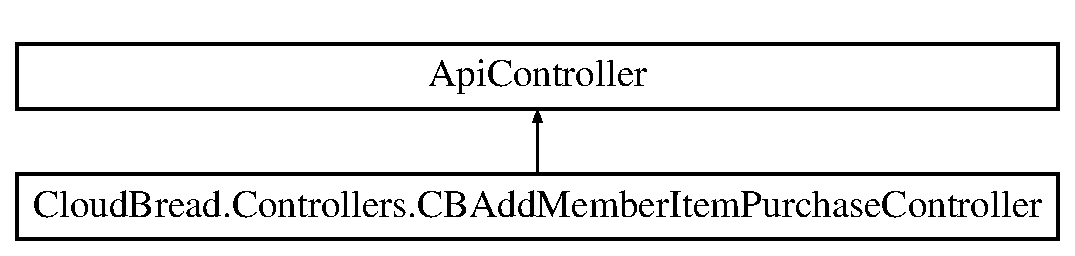
\includegraphics[height=2.000000cm]{a00006}
\end{center}
\end{figure}
\subsection*{Public Member Functions}
\begin{DoxyCompactItemize}
\item 
Http\+Response\+Message \hyperlink{a00006_a903454abbe81ed54ba7c99cfa684c3ad}{Post} (\hyperlink{a00004}{Add\+Member\+Item\+Purchase\+Input\+Params} p)
\end{DoxyCompactItemize}


\subsection{Member Function Documentation}
\index{Cloud\+Bread\+::\+Controllers\+::\+C\+B\+Add\+Member\+Item\+Purchase\+Controller@{Cloud\+Bread\+::\+Controllers\+::\+C\+B\+Add\+Member\+Item\+Purchase\+Controller}!Post@{Post}}
\index{Post@{Post}!Cloud\+Bread\+::\+Controllers\+::\+C\+B\+Add\+Member\+Item\+Purchase\+Controller@{Cloud\+Bread\+::\+Controllers\+::\+C\+B\+Add\+Member\+Item\+Purchase\+Controller}}
\subsubsection[{\texorpdfstring{Post(\+Add\+Member\+Item\+Purchase\+Input\+Params p)}{Post(AddMemberItemPurchaseInputParams p)}}]{\setlength{\rightskip}{0pt plus 5cm}Http\+Response\+Message Cloud\+Bread.\+Controllers.\+C\+B\+Add\+Member\+Item\+Purchase\+Controller.\+Post (
\begin{DoxyParamCaption}
\item[{{\bf Add\+Member\+Item\+Purchase\+Input\+Params}}]{p}
\end{DoxyParamCaption}
)}\hypertarget{a00006_a903454abbe81ed54ba7c99cfa684c3ad}{}\label{a00006_a903454abbe81ed54ba7c99cfa684c3ad}
Database connection retry policy

Encrypt the result response 

The documentation for this class was generated from the following file\+:\begin{DoxyCompactItemize}
\item 
C\+:/\+Users/dwkim/\+Documents/\+Git\+Hub/\+Cloud\+Bread/\+Controllers/\hyperlink{a00119}{C\+B\+Add\+Member\+Item\+Purchase\+Controller.\+cs}\end{DoxyCompactItemize}

\hypertarget{a00007}{}\section{Cloud\+Bread.\+Controllers.\+C\+B\+Add\+Use\+Member\+Item\+Controller Class Reference}
\label{a00007}\index{Cloud\+Bread.\+Controllers.\+C\+B\+Add\+Use\+Member\+Item\+Controller@{Cloud\+Bread.\+Controllers.\+C\+B\+Add\+Use\+Member\+Item\+Controller}}
Inheritance diagram for Cloud\+Bread.\+Controllers.\+C\+B\+Add\+Use\+Member\+Item\+Controller\+:\begin{figure}[H]
\begin{center}
\leavevmode
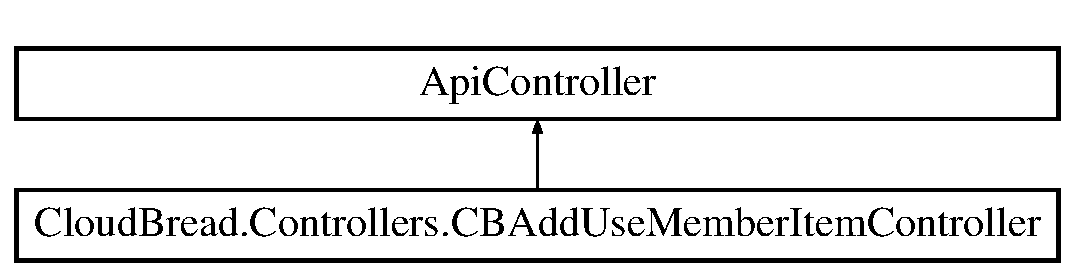
\includegraphics[height=2.000000cm]{a00007}
\end{center}
\end{figure}
\subsection*{Public Member Functions}
\begin{DoxyCompactItemize}
\item 
Http\+Response\+Message \hyperlink{a00007_ab5788c7ca4c3cfaadae7f8557bb8adcf}{Post} (\hyperlink{a00005}{Add\+Use\+Member\+Item\+Input\+Params} p)
\end{DoxyCompactItemize}


\subsection{Member Function Documentation}
\index{Cloud\+Bread\+::\+Controllers\+::\+C\+B\+Add\+Use\+Member\+Item\+Controller@{Cloud\+Bread\+::\+Controllers\+::\+C\+B\+Add\+Use\+Member\+Item\+Controller}!Post@{Post}}
\index{Post@{Post}!Cloud\+Bread\+::\+Controllers\+::\+C\+B\+Add\+Use\+Member\+Item\+Controller@{Cloud\+Bread\+::\+Controllers\+::\+C\+B\+Add\+Use\+Member\+Item\+Controller}}
\subsubsection[{\texorpdfstring{Post(\+Add\+Use\+Member\+Item\+Input\+Params p)}{Post(AddUseMemberItemInputParams p)}}]{\setlength{\rightskip}{0pt plus 5cm}Http\+Response\+Message Cloud\+Bread.\+Controllers.\+C\+B\+Add\+Use\+Member\+Item\+Controller.\+Post (
\begin{DoxyParamCaption}
\item[{{\bf Add\+Use\+Member\+Item\+Input\+Params}}]{p}
\end{DoxyParamCaption}
)}\hypertarget{a00007_ab5788c7ca4c3cfaadae7f8557bb8adcf}{}\label{a00007_ab5788c7ca4c3cfaadae7f8557bb8adcf}
Database connection retry policy

Encrypt the result response 

The documentation for this class was generated from the following file\+:\begin{DoxyCompactItemize}
\item 
C\+:/\+Users/dwkim/\+Documents/\+Git\+Hub/\+Cloud\+Bread/\+Controllers/\hyperlink{a00120}{C\+B\+Add\+Use\+Member\+Item\+Controller.\+cs}\end{DoxyCompactItemize}

\hypertarget{a00008}{}\section{Logger.\+Logging.\+Logging.\+C\+B\+A\+T\+S\+Message\+Entity Class Reference}
\label{a00008}\index{Logger.\+Logging.\+Logging.\+C\+B\+A\+T\+S\+Message\+Entity@{Logger.\+Logging.\+Logging.\+C\+B\+A\+T\+S\+Message\+Entity}}


Entity class for log structure -\/ including A\+TS ~\newline
.  


Inheritance diagram for Logger.\+Logging.\+Logging.\+C\+B\+A\+T\+S\+Message\+Entity\+:\begin{figure}[H]
\begin{center}
\leavevmode
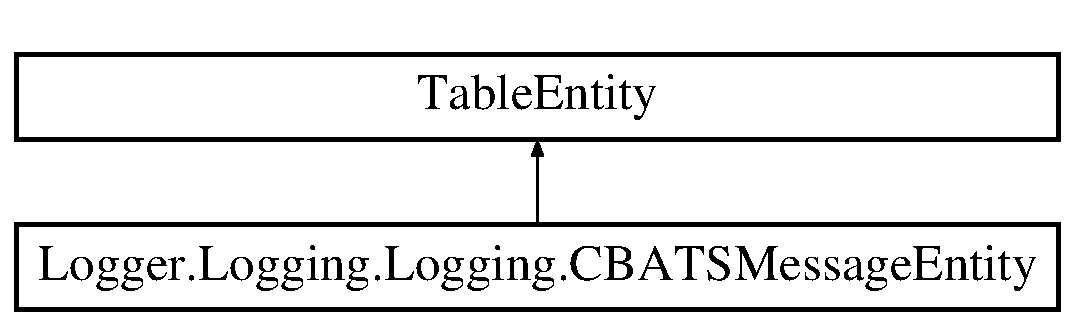
\includegraphics[height=2.000000cm]{a00008}
\end{center}
\end{figure}
\subsection*{Public Member Functions}
\begin{DoxyCompactItemize}
\item 
{\bfseries C\+B\+A\+T\+S\+Message\+Entity} (string pkey, string rkey)\hypertarget{a00008_ac00d1ec7e6dd95b76bd5a2d21ec821f3}{}\label{a00008_ac00d1ec7e6dd95b76bd5a2d21ec821f3}

\end{DoxyCompactItemize}
\subsection*{Properties}
\begin{DoxyCompactItemize}
\item 
string {\bfseries Member\+ID}\hspace{0.3cm}{\ttfamily  \mbox{[}get, set\mbox{]}}\hypertarget{a00008_a382e263ec656efb85732783bc41e9fb6}{}\label{a00008_a382e263ec656efb85732783bc41e9fb6}

\item 
string {\bfseries job\+ID}\hspace{0.3cm}{\ttfamily  \mbox{[}get, set\mbox{]}}\hypertarget{a00008_a0f39a8652da22a2fbfedfc917f473477}{}\label{a00008_a0f39a8652da22a2fbfedfc917f473477}

\item 
string {\bfseries Date}\hspace{0.3cm}{\ttfamily  \mbox{[}get, set\mbox{]}}\hypertarget{a00008_a1ea76e75065ee60b13bdeaa82379f47e}{}\label{a00008_a1ea76e75065ee60b13bdeaa82379f47e}

\item 
string {\bfseries Thread}\hspace{0.3cm}{\ttfamily  \mbox{[}get, set\mbox{]}}\hypertarget{a00008_aed296cea4c39b196d84c796aea76bfcb}{}\label{a00008_aed296cea4c39b196d84c796aea76bfcb}

\item 
string {\bfseries Level}\hspace{0.3cm}{\ttfamily  \mbox{[}get, set\mbox{]}}\hypertarget{a00008_a1a502760a55df247634f3f48ed2d5a14}{}\label{a00008_a1a502760a55df247634f3f48ed2d5a14}

\item 
string {\bfseries Logger}\hspace{0.3cm}{\ttfamily  \mbox{[}get, set\mbox{]}}\hypertarget{a00008_ae021ff6724db63e9a611aa1a1179ea60}{}\label{a00008_ae021ff6724db63e9a611aa1a1179ea60}

\item 
string {\bfseries Message}\hspace{0.3cm}{\ttfamily  \mbox{[}get, set\mbox{]}}\hypertarget{a00008_af0c7de3a2171d335546b86c0751ecac4}{}\label{a00008_af0c7de3a2171d335546b86c0751ecac4}

\item 
string {\bfseries Exception}\hspace{0.3cm}{\ttfamily  \mbox{[}get, set\mbox{]}}\hypertarget{a00008_a72d3258601bee8024c54bbe377427f28}{}\label{a00008_a72d3258601bee8024c54bbe377427f28}

\end{DoxyCompactItemize}


\subsection{Detailed Description}
Entity class for log structure -\/ including A\+TS ~\newline
. 

The documentation for this class was generated from the following file\+:\begin{DoxyCompactItemize}
\item 
C\+:/\+Users/dwkim/\+Documents/\+Git\+Hub/\+Cloud\+Bread/C\+B\+Loggers.\+cs\end{DoxyCompactItemize}

\hypertarget{a00009}{}\section{Cloud\+Bread\+Admin\+Web.\+Admin\+Member\+Login.\+Models.\+Controllers.\+Admin\+Login\+Controller Class Reference}
\label{a00009}\index{Cloud\+Bread\+Admin\+Web.\+Admin\+Member\+Login.\+Models.\+Controllers.\+Admin\+Login\+Controller@{Cloud\+Bread\+Admin\+Web.\+Admin\+Member\+Login.\+Models.\+Controllers.\+Admin\+Login\+Controller}}
Inheritance diagram for Cloud\+Bread\+Admin\+Web.\+Admin\+Member\+Login.\+Models.\+Controllers.\+Admin\+Login\+Controller\+:\begin{figure}[H]
\begin{center}
\leavevmode
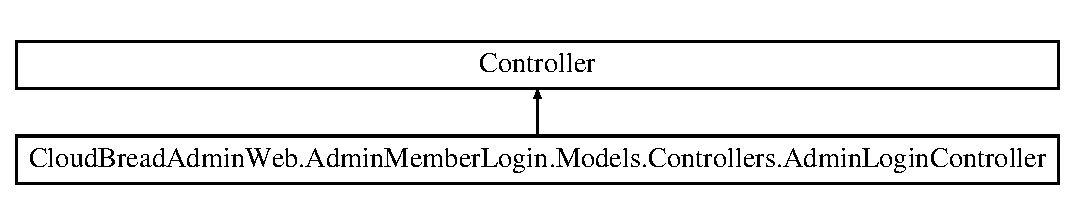
\includegraphics[height=2.000000cm]{a00009}
\end{center}
\end{figure}
\subsection*{Public Member Functions}
\begin{DoxyCompactItemize}
\item 
Action\+Result {\bfseries Index} ()\hypertarget{a00009_a6a86ef816be4f0469f4a305f5dd6ecf2}{}\label{a00009_a6a86ef816be4f0469f4a305f5dd6ecf2}

\item 
Action\+Result {\bfseries Login} ()\hypertarget{a00009_a2bc2253d4535bb67490f8b5cc1ee84b7}{}\label{a00009_a2bc2253d4535bb67490f8b5cc1ee84b7}

\item 
Action\+Result {\bfseries Login} (\hyperlink{a00010}{Models.\+Admin\+Member\+Login} user)\hypertarget{a00009_a635757af63e9798fd3db50b278876d1e}{}\label{a00009_a635757af63e9798fd3db50b278876d1e}

\item 
Action\+Result {\bfseries Logout} (\hyperlink{a00011}{Cloud\+Bread\+Admin\+Web.\+Admin\+Member\+Logout.\+Models.\+Admin\+Member\+Logout} Admin)\hypertarget{a00009_a4a8d0c87d51f509f1185c13223d623f4}{}\label{a00009_a4a8d0c87d51f509f1185c13223d623f4}

\end{DoxyCompactItemize}


The documentation for this class was generated from the following file\+:\begin{DoxyCompactItemize}
\item 
C\+:/\+Users/dwkim/\+Documents/\+Git\+Hub/\+Cloud\+Bread/\+Cloud\+Bread\+Admin\+Web/\+Controllers/Admin\+Login\+Controller.\+cs\end{DoxyCompactItemize}

\hypertarget{a00010}{}\section{Cloud\+Bread\+Admin\+Web.\+Admin\+Member\+Login.\+Models.\+Admin\+Member\+Login Class Reference}
\label{a00010}\index{Cloud\+Bread\+Admin\+Web.\+Admin\+Member\+Login.\+Models.\+Admin\+Member\+Login@{Cloud\+Bread\+Admin\+Web.\+Admin\+Member\+Login.\+Models.\+Admin\+Member\+Login}}
\subsection*{Classes}
\begin{DoxyCompactItemize}
\item 
class \hyperlink{a00152}{Model}
\end{DoxyCompactItemize}
\subsection*{Public Member Functions}
\begin{DoxyCompactItemize}
\item 
List$<$ \hyperlink{a00152}{Model} $>$ {\bfseries C\+B\+Admin\+Login} (string user\+Name, string pass\+Word, string ip\+Address)\hypertarget{a00010_a63d8f50572b6c2bd5c6cd8514f3c696e}{}\label{a00010_a63d8f50572b6c2bd5c6cd8514f3c696e}

\end{DoxyCompactItemize}
\subsection*{Properties}
\begin{DoxyCompactItemize}
\item 
string {\bfseries User\+Name}\hspace{0.3cm}{\ttfamily  \mbox{[}get, set\mbox{]}}\hypertarget{a00010_ad0d90ff54cd8ffc4270b7e093c3bddbd}{}\label{a00010_ad0d90ff54cd8ffc4270b7e093c3bddbd}

\item 
string {\bfseries Password}\hspace{0.3cm}{\ttfamily  \mbox{[}get, set\mbox{]}}\hypertarget{a00010_a3604082f7c0c90e30d160d41797ca619}{}\label{a00010_a3604082f7c0c90e30d160d41797ca619}

\end{DoxyCompactItemize}


The documentation for this class was generated from the following file\+:\begin{DoxyCompactItemize}
\item 
C\+:/\+Users/dwkim/\+Documents/\+Git\+Hub/\+Cloud\+Bread/\+Cloud\+Bread\+Admin\+Web/\+Data\+Objects/Admin\+Member\+Login.\+cs\end{DoxyCompactItemize}

\hypertarget{a00011}{}\section{Cloud\+Bread\+Admin\+Web.\+Admin\+Member\+Logout.\+Models.\+Admin\+Member\+Logout Class Reference}
\label{a00011}\index{Cloud\+Bread\+Admin\+Web.\+Admin\+Member\+Logout.\+Models.\+Admin\+Member\+Logout@{Cloud\+Bread\+Admin\+Web.\+Admin\+Member\+Logout.\+Models.\+Admin\+Member\+Logout}}
\subsection*{Classes}
\begin{DoxyCompactItemize}
\item 
class \hyperlink{a00161}{Model}
\end{DoxyCompactItemize}
\subsection*{Public Member Functions}
\begin{DoxyCompactItemize}
\item 
string {\bfseries C\+B\+Admin\+Logout} (string admin\+Member\+ID)\hypertarget{a00011_a6d6217d3c644febc1d52adb1c66756cc}{}\label{a00011_a6d6217d3c644febc1d52adb1c66756cc}

\end{DoxyCompactItemize}
\subsection*{Properties}
\begin{DoxyCompactItemize}
\item 
string {\bfseries Admin\+Member\+ID}\hspace{0.3cm}{\ttfamily  \mbox{[}get, set\mbox{]}}\hypertarget{a00011_a58f35da010d962811a25a4ce6b7a34d5}{}\label{a00011_a58f35da010d962811a25a4ce6b7a34d5}

\end{DoxyCompactItemize}


The documentation for this class was generated from the following file\+:\begin{DoxyCompactItemize}
\item 
C\+:/\+Users/dwkim/\+Documents/\+Git\+Hub/\+Cloud\+Bread/\+Cloud\+Bread\+Admin\+Web/\+Data\+Objects/Admin\+Member\+Logout.\+cs\end{DoxyCompactItemize}

\hypertarget{a00012}{}\section{Cloud\+Bread.\+Controllers.\+C\+B\+Com\+Ins\+Member\+Item\+Purchase\+Controller Class Reference}
\label{a00012}\index{Cloud\+Bread.\+Controllers.\+C\+B\+Com\+Ins\+Member\+Item\+Purchase\+Controller@{Cloud\+Bread.\+Controllers.\+C\+B\+Com\+Ins\+Member\+Item\+Purchase\+Controller}}
Inheritance diagram for Cloud\+Bread.\+Controllers.\+C\+B\+Com\+Ins\+Member\+Item\+Purchase\+Controller\+:\begin{figure}[H]
\begin{center}
\leavevmode
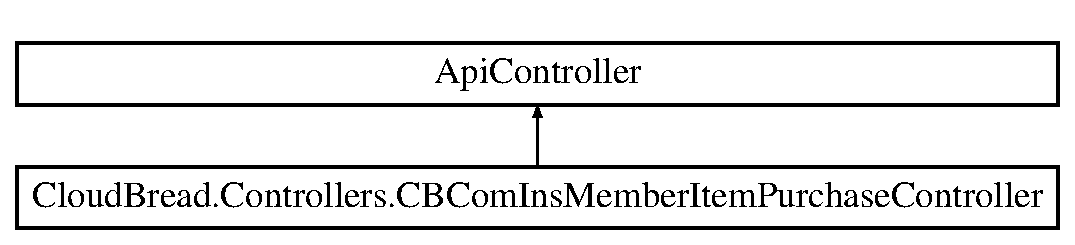
\includegraphics[height=2.000000cm]{a00012}
\end{center}
\end{figure}
\subsection*{Public Member Functions}
\begin{DoxyCompactItemize}
\item 
Http\+Response\+Message \hyperlink{a00012_a44a5a5bfa258980f426ff61e4572981d}{Post} (\hyperlink{a00051}{Com\+Ins\+Member\+Item\+Purchase\+Input\+Params} p)
\end{DoxyCompactItemize}


\subsection{Member Function Documentation}
\index{Cloud\+Bread\+::\+Controllers\+::\+C\+B\+Com\+Ins\+Member\+Item\+Purchase\+Controller@{Cloud\+Bread\+::\+Controllers\+::\+C\+B\+Com\+Ins\+Member\+Item\+Purchase\+Controller}!Post@{Post}}
\index{Post@{Post}!Cloud\+Bread\+::\+Controllers\+::\+C\+B\+Com\+Ins\+Member\+Item\+Purchase\+Controller@{Cloud\+Bread\+::\+Controllers\+::\+C\+B\+Com\+Ins\+Member\+Item\+Purchase\+Controller}}
\subsubsection[{\texorpdfstring{Post(\+Com\+Ins\+Member\+Item\+Purchase\+Input\+Params p)}{Post(ComInsMemberItemPurchaseInputParams p)}}]{\setlength{\rightskip}{0pt plus 5cm}Http\+Response\+Message Cloud\+Bread.\+Controllers.\+C\+B\+Com\+Ins\+Member\+Item\+Purchase\+Controller.\+Post (
\begin{DoxyParamCaption}
\item[{{\bf Com\+Ins\+Member\+Item\+Purchase\+Input\+Params}}]{p}
\end{DoxyParamCaption}
)}\hypertarget{a00012_a44a5a5bfa258980f426ff61e4572981d}{}\label{a00012_a44a5a5bfa258980f426ff61e4572981d}
Database connection retry policy

Encrypt the result response 

The documentation for this class was generated from the following file\+:\begin{DoxyCompactItemize}
\item 
C\+:/\+Users/dwkim/\+Documents/\+Git\+Hub/\+Cloud\+Bread/\+Controllers/C\+B\+Com\+Ins\+Member\+Item\+Purchase\+Controller\+Controller.\+cs\end{DoxyCompactItemize}

\hypertarget{a00013}{}\section{Cloud\+Bread.\+Controllers.\+C\+B\+Com\+Sel\+Coupon\+Controller Class Reference}
\label{a00013}\index{Cloud\+Bread.\+Controllers.\+C\+B\+Com\+Sel\+Coupon\+Controller@{Cloud\+Bread.\+Controllers.\+C\+B\+Com\+Sel\+Coupon\+Controller}}
Inheritance diagram for Cloud\+Bread.\+Controllers.\+C\+B\+Com\+Sel\+Coupon\+Controller\+:\begin{figure}[H]
\begin{center}
\leavevmode
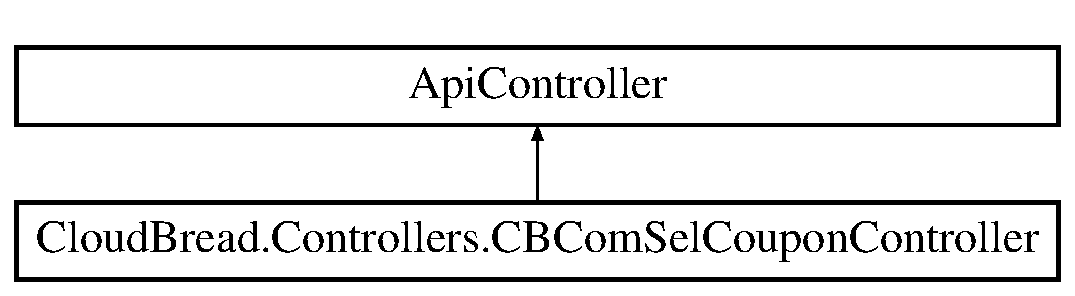
\includegraphics[height=2.000000cm]{a00013}
\end{center}
\end{figure}
\subsection*{Public Member Functions}
\begin{DoxyCompactItemize}
\item 
Http\+Response\+Message \hyperlink{a00013_ab0c5d66b516d261d981d47e6029b3178}{Post} (\hyperlink{a00052}{Com\+Sel\+Coupon\+Input\+Params} p)
\end{DoxyCompactItemize}


\subsection{Member Function Documentation}
\index{Cloud\+Bread\+::\+Controllers\+::\+C\+B\+Com\+Sel\+Coupon\+Controller@{Cloud\+Bread\+::\+Controllers\+::\+C\+B\+Com\+Sel\+Coupon\+Controller}!Post@{Post}}
\index{Post@{Post}!Cloud\+Bread\+::\+Controllers\+::\+C\+B\+Com\+Sel\+Coupon\+Controller@{Cloud\+Bread\+::\+Controllers\+::\+C\+B\+Com\+Sel\+Coupon\+Controller}}
\subsubsection[{\texorpdfstring{Post(\+Com\+Sel\+Coupon\+Input\+Params p)}{Post(ComSelCouponInputParams p)}}]{\setlength{\rightskip}{0pt plus 5cm}Http\+Response\+Message Cloud\+Bread.\+Controllers.\+C\+B\+Com\+Sel\+Coupon\+Controller.\+Post (
\begin{DoxyParamCaption}
\item[{{\bf Com\+Sel\+Coupon\+Input\+Params}}]{p}
\end{DoxyParamCaption}
)}\hypertarget{a00013_ab0c5d66b516d261d981d47e6029b3178}{}\label{a00013_ab0c5d66b516d261d981d47e6029b3178}
Database connection retry policy

Encrypt the result response 

The documentation for this class was generated from the following file\+:\begin{DoxyCompactItemize}
\item 
C\+:/\+Users/dwkim/\+Documents/\+Git\+Hub/\+Cloud\+Bread/\+Controllers/\hyperlink{a00124}{C\+B\+Com\+Sel\+Coupon\+Controller.\+cs}\end{DoxyCompactItemize}

\hypertarget{a00014}{}\section{com.\+example.\+dwtechdaysdemo.\+A\+E\+S256\+Cipher Class Reference}
\label{a00014}\index{com.\+example.\+dwtechdaysdemo.\+A\+E\+S256\+Cipher@{com.\+example.\+dwtechdaysdemo.\+A\+E\+S256\+Cipher}}
\subsection*{Static Public Member Functions}
\begin{DoxyCompactItemize}
\item 
static String {\bfseries A\+E\+S\+\_\+\+Encode} (String str, String key)  throws java.\+io.\+Unsupported\+Encoding\+Exception, No\+Such\+Algorithm\+Exception, No\+Such\+Padding\+Exception, Invalid\+Key\+Exception, Invalid\+Algorithm\+Parameter\+Exception,	\+Illegal\+Block\+Size\+Exception, Bad\+Padding\+Exception \hypertarget{a00014_a97f7c104da946fe9b28e7bb68b5ba607}{}\label{a00014_a97f7c104da946fe9b28e7bb68b5ba607}

\item 
static String {\bfseries A\+E\+S\+\_\+\+Decode} (String str, String key)  throws java.\+io.\+Unsupported\+Encoding\+Exception, No\+Such\+Algorithm\+Exception, No\+Such\+Padding\+Exception, Invalid\+Key\+Exception, Invalid\+Algorithm\+Parameter\+Exception, Illegal\+Block\+Size\+Exception, Bad\+Padding\+Exception \hypertarget{a00014_a7a122dbded6e7fc850a069c4864336e1}{}\label{a00014_a7a122dbded6e7fc850a069c4864336e1}

\end{DoxyCompactItemize}
\subsection*{Static Public Attributes}
\begin{DoxyCompactItemize}
\item 
static byte\mbox{[}$\,$\mbox{]} {\bfseries iv\+Bytes} = \{ 0x00, 0x00, 0x00, 0x00, 0x00, 0x00, 0x00, 0x00, 0x00, 0x00, 0x00, 0x00, 0x00, 0x00, 0x00, 0x00 \}\hypertarget{a00014_a7851e04c17d2133f4c66b8ce11cad199}{}\label{a00014_a7851e04c17d2133f4c66b8ce11cad199}

\item 
static byte\mbox{[}$\,$\mbox{]} {\bfseries key\+Bytes} = \{ 0x00, 0x00, 0x00, 0x00, 0x00, 0x00, 0x00, 0x00, 0x00, 0x00, 0x00, 0x00, 0x00, 0x00, 0x00, 0x00 \}\hypertarget{a00014_a595598295e8b7294b71f528029b3c09f}{}\label{a00014_a595598295e8b7294b71f528029b3c09f}

\end{DoxyCompactItemize}


The documentation for this class was generated from the following file\+:\begin{DoxyCompactItemize}
\item 
C\+:/\+Users/dwkim/\+Documents/\+Git\+Hub/\+Cloud\+Bread/\+Tools/\+Android\+\_\+\+Test\+App\+\_\+\+Cloud\+Bread/src/com/example/dwtechdaysdemo/A\+E\+S256\+Cipher.\+java\end{DoxyCompactItemize}

\hypertarget{a00015}{}\section{Cloud\+Bread\+Windows\+Store\+App\+Test\+Tool.\+App Class Reference}
\label{a00015}\index{Cloud\+Bread\+Windows\+Store\+App\+Test\+Tool.\+App@{Cloud\+Bread\+Windows\+Store\+App\+Test\+Tool.\+App}}


기본 응용 프로그램 클래스를 보완하는 응용 프로그램별 동작을 제공합니다.  


Inheritance diagram for Cloud\+Bread\+Windows\+Store\+App\+Test\+Tool.\+App\+:\begin{figure}[H]
\begin{center}
\leavevmode
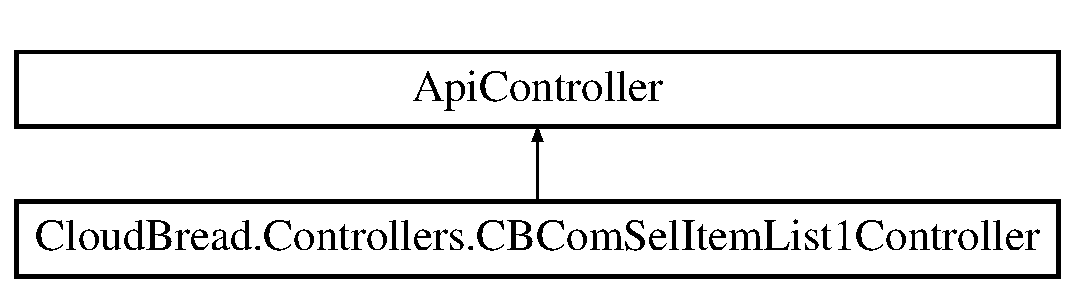
\includegraphics[height=0.707071cm]{a00015}
\end{center}
\end{figure}
\subsection*{Public Member Functions}
\begin{DoxyCompactItemize}
\item 
\hyperlink{a00015_a1719bb741c5cfb24b6745cd2b9172bd8}{App} ()
\begin{DoxyCompactList}\small\item\em Singleton 응용 프로그램 개체를 초기화합니다. 이것은 실행되는 작성 코드의 첫 번째 줄이며 따라서 main() 또는 Win\+Main()과 논리적으로 동일합니다. \end{DoxyCompactList}\item 
void {\bfseries Connect} (int connection\+Id, object target)\hypertarget{a00015_aa0b90b9ef72df1b4b04b989765843170}{}\label{a00015_aa0b90b9ef72df1b4b04b989765843170}

\item 
void {\bfseries Initialize\+Component} ()\hypertarget{a00015_a8956af89a6c67e881e14444a106aa2a0}{}\label{a00015_a8956af89a6c67e881e14444a106aa2a0}

\item 
global\+::\+Windows.\+U\+I.\+Xaml.\+Markup.\+I\+Xaml\+Type {\bfseries Get\+Xaml\+Type} (global\+::\+System.\+Type type)\hypertarget{a00015_ab857c47c2dd1871550b33aa1db3065d7}{}\label{a00015_ab857c47c2dd1871550b33aa1db3065d7}

\item 
global\+::\+Windows.\+U\+I.\+Xaml.\+Markup.\+I\+Xaml\+Type {\bfseries Get\+Xaml\+Type} (string full\+Name)\hypertarget{a00015_a8bec7c4a0cd7ae2cfcfd21d87b96d308}{}\label{a00015_a8bec7c4a0cd7ae2cfcfd21d87b96d308}

\item 
global\+::\+Windows.\+U\+I.\+Xaml.\+Markup.\+Xmlns\+Definition\mbox{[}$\,$\mbox{]} {\bfseries Get\+Xmlns\+Definitions} ()\hypertarget{a00015_aec8eef3d490b093f325f842569bee9c5}{}\label{a00015_aec8eef3d490b093f325f842569bee9c5}

\item 
void {\bfseries Initialize\+Component} ()\hypertarget{a00015_a8956af89a6c67e881e14444a106aa2a0}{}\label{a00015_a8956af89a6c67e881e14444a106aa2a0}

\end{DoxyCompactItemize}
\subsection*{Protected Member Functions}
\begin{DoxyCompactItemize}
\item 
override void \hyperlink{a00015_aaf786277b3444f9117fd7d14d247d412}{On\+Launched} (Launch\+Activated\+Event\+Args e)
\begin{DoxyCompactList}\small\item\em 최종 사용자가 응용 프로그램을 정상적으로 시작할 때 호출됩니다. 다른 진입점은 응용 프로그램에서 특정 파일을 열기 시작할 때 사용됩니다. \end{DoxyCompactList}\end{DoxyCompactItemize}


\subsection{Detailed Description}
기본 응용 프로그램 클래스를 보완하는 응용 프로그램별 동작을 제공합니다. 



\subsection{Constructor \& Destructor Documentation}
\index{Cloud\+Bread\+Windows\+Store\+App\+Test\+Tool\+::\+App@{Cloud\+Bread\+Windows\+Store\+App\+Test\+Tool\+::\+App}!App@{App}}
\index{App@{App}!Cloud\+Bread\+Windows\+Store\+App\+Test\+Tool\+::\+App@{Cloud\+Bread\+Windows\+Store\+App\+Test\+Tool\+::\+App}}
\subsubsection[{\texorpdfstring{App()}{App()}}]{\setlength{\rightskip}{0pt plus 5cm}Cloud\+Bread\+Windows\+Store\+App\+Test\+Tool.\+App.\+App (
\begin{DoxyParamCaption}
{}
\end{DoxyParamCaption}
)}\hypertarget{a00015_a1719bb741c5cfb24b6745cd2b9172bd8}{}\label{a00015_a1719bb741c5cfb24b6745cd2b9172bd8}


Singleton 응용 프로그램 개체를 초기화합니다. 이것은 실행되는 작성 코드의 첫 번째 줄이며 따라서 main() 또는 Win\+Main()과 논리적으로 동일합니다. 



\subsection{Member Function Documentation}
\index{Cloud\+Bread\+Windows\+Store\+App\+Test\+Tool\+::\+App@{Cloud\+Bread\+Windows\+Store\+App\+Test\+Tool\+::\+App}!On\+Launched@{On\+Launched}}
\index{On\+Launched@{On\+Launched}!Cloud\+Bread\+Windows\+Store\+App\+Test\+Tool\+::\+App@{Cloud\+Bread\+Windows\+Store\+App\+Test\+Tool\+::\+App}}
\subsubsection[{\texorpdfstring{On\+Launched(\+Launch\+Activated\+Event\+Args e)}{OnLaunched(LaunchActivatedEventArgs e)}}]{\setlength{\rightskip}{0pt plus 5cm}override void Cloud\+Bread\+Windows\+Store\+App\+Test\+Tool.\+App.\+On\+Launched (
\begin{DoxyParamCaption}
\item[{Launch\+Activated\+Event\+Args}]{e}
\end{DoxyParamCaption}
)\hspace{0.3cm}{\ttfamily [protected]}}\hypertarget{a00015_aaf786277b3444f9117fd7d14d247d412}{}\label{a00015_aaf786277b3444f9117fd7d14d247d412}


최종 사용자가 응용 프로그램을 정상적으로 시작할 때 호출됩니다. 다른 진입점은 응용 프로그램에서 특정 파일을 열기 시작할 때 사용됩니다. 


\begin{DoxyParams}{Parameters}
{\em e} & 시작 요청 및 프로세스에 대한 정보입니다.\\
\hline
\end{DoxyParams}


The documentation for this class was generated from the following files\+:\begin{DoxyCompactItemize}
\item 
C\+:/\+Users/dwkim/\+Documents/\+Git\+Hub/\+Cloud\+Bread/\+Cloud\+Bread\+Windows\+Store\+App\+Test\+Tool/App.\+xaml.\+cs\item 
C\+:/\+Users/dwkim/\+Documents/\+Git\+Hub/\+Cloud\+Bread/\+Cloud\+Bread\+Windows\+Store\+App\+Test\+Tool/obj/\+Debug/App.\+g.\+i.\+cs\item 
C\+:/\+Users/dwkim/\+Documents/\+Git\+Hub/\+Cloud\+Bread/\+Cloud\+Bread\+Windows\+Store\+App\+Test\+Tool/obj/\+Debug/Xaml\+Type\+Info.\+g.\+cs\item 
C\+:/\+Users/dwkim/\+Documents/\+Git\+Hub/\+Cloud\+Bread/\+Cloud\+Bread\+Windows\+Store\+App\+Test\+Tool/obj/\+Debug/App.\+g.\+cs\end{DoxyCompactItemize}

\hypertarget{a00016}{}\section{Cloud\+Bread\+Admin\+Web.\+Models.\+Application\+Db\+Context Class Reference}
\label{a00016}\index{Cloud\+Bread\+Admin\+Web.\+Models.\+Application\+Db\+Context@{Cloud\+Bread\+Admin\+Web.\+Models.\+Application\+Db\+Context}}
Inheritance diagram for Cloud\+Bread\+Admin\+Web.\+Models.\+Application\+Db\+Context\+:\begin{figure}[H]
\begin{center}
\leavevmode
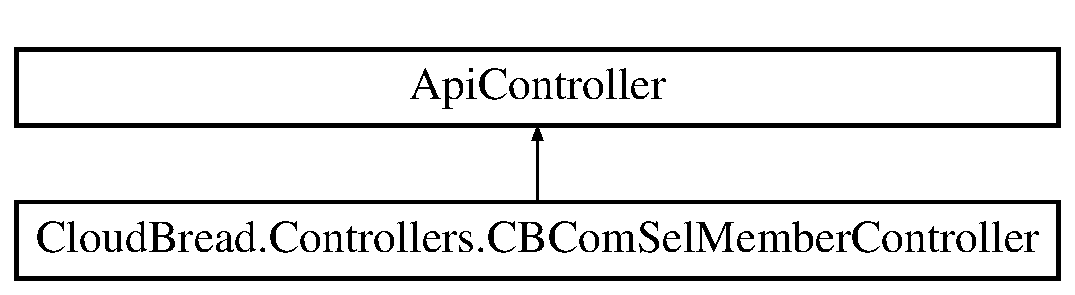
\includegraphics[height=2.000000cm]{a00016}
\end{center}
\end{figure}
\subsection*{Static Public Member Functions}
\begin{DoxyCompactItemize}
\item 
static \hyperlink{a00016}{Application\+Db\+Context} {\bfseries Create} ()\hypertarget{a00016_ae838c6a49ec5da37448d58c0b7ea9fed}{}\label{a00016_ae838c6a49ec5da37448d58c0b7ea9fed}

\end{DoxyCompactItemize}


The documentation for this class was generated from the following file\+:\begin{DoxyCompactItemize}
\item 
C\+:/\+Users/dwkim/\+Documents/\+Git\+Hub/\+Cloud\+Bread/\+Cloud\+Bread\+Admin\+Web/\+Models/Identity\+Models.\+cs\end{DoxyCompactItemize}

\hypertarget{a00017}{}\section{Cloud\+Bread.\+Controllers.\+C\+B\+Com\+Sel\+Member\+Game\+Infoes\+Controller Class Reference}
\label{a00017}\index{Cloud\+Bread.\+Controllers.\+C\+B\+Com\+Sel\+Member\+Game\+Infoes\+Controller@{Cloud\+Bread.\+Controllers.\+C\+B\+Com\+Sel\+Member\+Game\+Infoes\+Controller}}
Inheritance diagram for Cloud\+Bread.\+Controllers.\+C\+B\+Com\+Sel\+Member\+Game\+Infoes\+Controller\+:\begin{figure}[H]
\begin{center}
\leavevmode
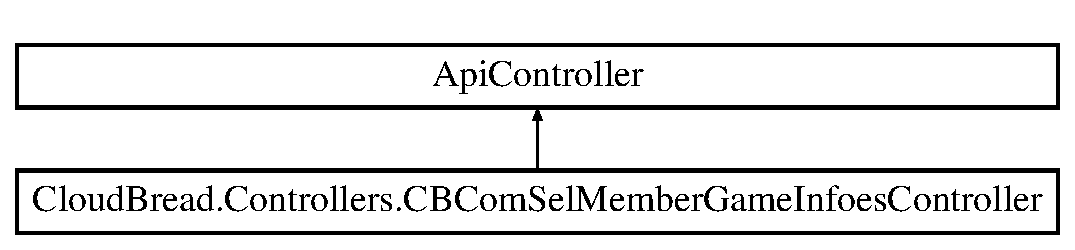
\includegraphics[height=2.000000cm]{a00017}
\end{center}
\end{figure}
\subsection*{Public Member Functions}
\begin{DoxyCompactItemize}
\item 
Http\+Response\+Message \hyperlink{a00017_a0a12cb0713f328a9bb262c1a4170bab8}{Post} (\hyperlink{a00058}{Com\+Sel\+Member\+Game\+Infoes\+Input\+Params} p)
\end{DoxyCompactItemize}


\subsection{Member Function Documentation}
\index{Cloud\+Bread\+::\+Controllers\+::\+C\+B\+Com\+Sel\+Member\+Game\+Infoes\+Controller@{Cloud\+Bread\+::\+Controllers\+::\+C\+B\+Com\+Sel\+Member\+Game\+Infoes\+Controller}!Post@{Post}}
\index{Post@{Post}!Cloud\+Bread\+::\+Controllers\+::\+C\+B\+Com\+Sel\+Member\+Game\+Infoes\+Controller@{Cloud\+Bread\+::\+Controllers\+::\+C\+B\+Com\+Sel\+Member\+Game\+Infoes\+Controller}}
\subsubsection[{\texorpdfstring{Post(\+Com\+Sel\+Member\+Game\+Infoes\+Input\+Params p)}{Post(ComSelMemberGameInfoesInputParams p)}}]{\setlength{\rightskip}{0pt plus 5cm}Http\+Response\+Message Cloud\+Bread.\+Controllers.\+C\+B\+Com\+Sel\+Member\+Game\+Infoes\+Controller.\+Post (
\begin{DoxyParamCaption}
\item[{{\bf Com\+Sel\+Member\+Game\+Infoes\+Input\+Params}}]{p}
\end{DoxyParamCaption}
)}\hypertarget{a00017_a0a12cb0713f328a9bb262c1a4170bab8}{}\label{a00017_a0a12cb0713f328a9bb262c1a4170bab8}
Database connection retry policy

Encrypt the result response 

The documentation for this class was generated from the following file\+:\begin{DoxyCompactItemize}
\item 
C\+:/\+Users/dwkim/\+Documents/\+Git\+Hub/\+Cloud\+Bread/\+Controllers/\hyperlink{a00128}{C\+B\+Com\+Sel\+Member\+Game\+Infoes\+Controller.\+cs}\end{DoxyCompactItemize}

\hypertarget{a00018}{}\section{Cloud\+Bread\+Admin\+Web.\+Models.\+Application\+User Class Reference}
\label{a00018}\index{Cloud\+Bread\+Admin\+Web.\+Models.\+Application\+User@{Cloud\+Bread\+Admin\+Web.\+Models.\+Application\+User}}
Inheritance diagram for Cloud\+Bread\+Admin\+Web.\+Models.\+Application\+User\+:\begin{figure}[H]
\begin{center}
\leavevmode
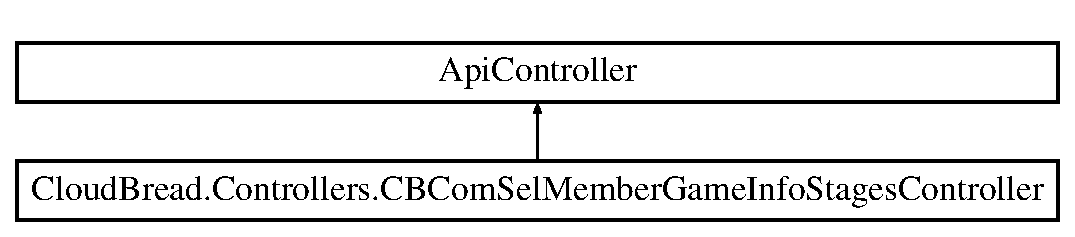
\includegraphics[height=2.000000cm]{a00018}
\end{center}
\end{figure}
\subsection*{Public Member Functions}
\begin{DoxyCompactItemize}
\item 
async Task$<$ Claims\+Identity $>$ {\bfseries Generate\+User\+Identity\+Async} (User\+Manager$<$ \hyperlink{a00018}{Application\+User} $>$ manager)\hypertarget{a00018_a18c626164316c53c14d4a2cc3b48bc45}{}\label{a00018_a18c626164316c53c14d4a2cc3b48bc45}

\end{DoxyCompactItemize}


The documentation for this class was generated from the following file\+:\begin{DoxyCompactItemize}
\item 
C\+:/\+Users/dwkim/\+Documents/\+Git\+Hub/\+Cloud\+Bread/\+Cloud\+Bread\+Admin\+Web/\+Models/Identity\+Models.\+cs\end{DoxyCompactItemize}

\hypertarget{a00019}{}\section{Cloud\+Bread\+Admin\+Web.\+Application\+User\+Manager Class Reference}
\label{a00019}\index{Cloud\+Bread\+Admin\+Web.\+Application\+User\+Manager@{Cloud\+Bread\+Admin\+Web.\+Application\+User\+Manager}}
Inheritance diagram for Cloud\+Bread\+Admin\+Web.\+Application\+User\+Manager\+:\begin{figure}[H]
\begin{center}
\leavevmode
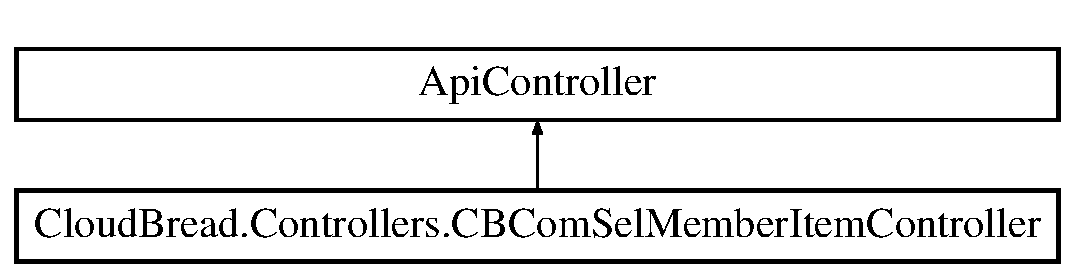
\includegraphics[height=2.000000cm]{a00019}
\end{center}
\end{figure}
\subsection*{Public Member Functions}
\begin{DoxyCompactItemize}
\item 
{\bfseries Application\+User\+Manager} (I\+User\+Store$<$ \hyperlink{a00018}{Application\+User} $>$ store)\hypertarget{a00019_ac64e803f424ca85090b245bcf18ec514}{}\label{a00019_ac64e803f424ca85090b245bcf18ec514}

\end{DoxyCompactItemize}
\subsection*{Static Public Member Functions}
\begin{DoxyCompactItemize}
\item 
static \hyperlink{a00019}{Application\+User\+Manager} {\bfseries Create} (Identity\+Factory\+Options$<$ \hyperlink{a00019}{Application\+User\+Manager} $>$ options, I\+Owin\+Context context)\hypertarget{a00019_ae2188287f4231a9b68f1204a634e97fd}{}\label{a00019_ae2188287f4231a9b68f1204a634e97fd}

\end{DoxyCompactItemize}


The documentation for this class was generated from the following file\+:\begin{DoxyCompactItemize}
\item 
C\+:/\+Users/dwkim/\+Documents/\+Git\+Hub/\+Cloud\+Bread/\+Cloud\+Bread\+Admin\+Web/\+App\+\_\+\+Start/Identity\+Config.\+cs\end{DoxyCompactItemize}

\hypertarget{a00020}{}\section{Cloud\+Bread\+Lib.\+B\+A\+L.\+Base64.\+Base64 Class Reference}
\label{a00020}\index{Cloud\+Bread\+Lib.\+B\+A\+L.\+Base64.\+Base64@{Cloud\+Bread\+Lib.\+B\+A\+L.\+Base64.\+Base64}}
\subsection*{Static Public Member Functions}
\begin{DoxyCompactItemize}
\item 
static string {\bfseries Base64\+Encode} (string plain\+Text)\hypertarget{a00020_a901a46986bd2fb9302c4cd728f09c2d4}{}\label{a00020_a901a46986bd2fb9302c4cd728f09c2d4}

\item 
static string {\bfseries Base64\+Decode} (string base64\+Encoded\+Data)\hypertarget{a00020_a56f06fb89cb0b7b03a4818cecc47b3aa}{}\label{a00020_a56f06fb89cb0b7b03a4818cecc47b3aa}

\end{DoxyCompactItemize}


The documentation for this class was generated from the following file\+:\begin{DoxyCompactItemize}
\item 
C\+:/\+Users/dwkim/\+Documents/\+Git\+Hub/\+Cloud\+Bread/\+Cloud\+Bread\+Lib/\+B\+A\+L/Base64.\+cs\end{DoxyCompactItemize}

\hypertarget{a00021}{}\section{com.\+example.\+dwtechdaysdemo.\+Build\+Config Class Reference}
\label{a00021}\index{com.\+example.\+dwtechdaysdemo.\+Build\+Config@{com.\+example.\+dwtechdaysdemo.\+Build\+Config}}
\subsection*{Static Public Attributes}
\begin{DoxyCompactItemize}
\item 
static final boolean {\bfseries D\+E\+B\+UG} = true\hypertarget{a00021_a50181a140684170980ee09094097c661}{}\label{a00021_a50181a140684170980ee09094097c661}

\end{DoxyCompactItemize}


The documentation for this class was generated from the following file\+:\begin{DoxyCompactItemize}
\item 
C\+:/\+Users/dwkim/\+Documents/\+Git\+Hub/\+Cloud\+Bread/\+Tools/\+Android\+\_\+\+Test\+App\+\_\+\+Cloud\+Bread/gen/com/example/dwtechdaysdemo/Build\+Config.\+java\end{DoxyCompactItemize}

\hypertarget{a00022}{}\section{Cloud\+Bread\+Admin\+Web.\+Bundle\+Config Class Reference}
\label{a00022}\index{Cloud\+Bread\+Admin\+Web.\+Bundle\+Config@{Cloud\+Bread\+Admin\+Web.\+Bundle\+Config}}
\subsection*{Static Public Member Functions}
\begin{DoxyCompactItemize}
\item 
static void {\bfseries Register\+Bundles} (Bundle\+Collection bundles)\hypertarget{a00022_a9533a2d4ad40e7376c4fa62b1cf1d47d}{}\label{a00022_a9533a2d4ad40e7376c4fa62b1cf1d47d}

\end{DoxyCompactItemize}


The documentation for this class was generated from the following file\+:\begin{DoxyCompactItemize}
\item 
C\+:/\+Users/dwkim/\+Documents/\+Git\+Hub/\+Cloud\+Bread/\+Cloud\+Bread\+Admin\+Web/\+App\+\_\+\+Start/Bundle\+Config.\+cs\end{DoxyCompactItemize}

\hypertarget{a00023}{}\section{Cloud\+Bread.\+Controllers.\+C\+B\+Com\+Udt\+Member\+Game\+Infoes\+Controller Class Reference}
\label{a00023}\index{Cloud\+Bread.\+Controllers.\+C\+B\+Com\+Udt\+Member\+Game\+Infoes\+Controller@{Cloud\+Bread.\+Controllers.\+C\+B\+Com\+Udt\+Member\+Game\+Infoes\+Controller}}
Inheritance diagram for Cloud\+Bread.\+Controllers.\+C\+B\+Com\+Udt\+Member\+Game\+Infoes\+Controller\+:\begin{figure}[H]
\begin{center}
\leavevmode
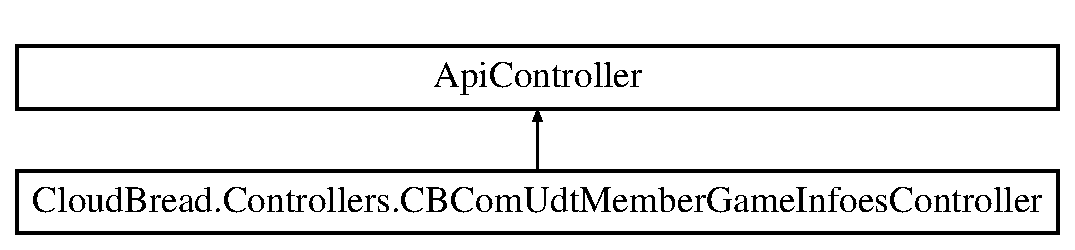
\includegraphics[height=2.000000cm]{a00023}
\end{center}
\end{figure}
\subsection*{Public Member Functions}
\begin{DoxyCompactItemize}
\item 
Http\+Response\+Message \hyperlink{a00023_affb75e25621e640f2015ba497fefe007}{Post} (\hyperlink{a00069}{Com\+Udt\+Member\+Game\+Infoes\+Input\+Params} p)
\end{DoxyCompactItemize}


\subsection{Member Function Documentation}
\index{Cloud\+Bread\+::\+Controllers\+::\+C\+B\+Com\+Udt\+Member\+Game\+Infoes\+Controller@{Cloud\+Bread\+::\+Controllers\+::\+C\+B\+Com\+Udt\+Member\+Game\+Infoes\+Controller}!Post@{Post}}
\index{Post@{Post}!Cloud\+Bread\+::\+Controllers\+::\+C\+B\+Com\+Udt\+Member\+Game\+Infoes\+Controller@{Cloud\+Bread\+::\+Controllers\+::\+C\+B\+Com\+Udt\+Member\+Game\+Infoes\+Controller}}
\subsubsection[{\texorpdfstring{Post(\+Com\+Udt\+Member\+Game\+Infoes\+Input\+Params p)}{Post(ComUdtMemberGameInfoesInputParams p)}}]{\setlength{\rightskip}{0pt plus 5cm}Http\+Response\+Message Cloud\+Bread.\+Controllers.\+C\+B\+Com\+Udt\+Member\+Game\+Infoes\+Controller.\+Post (
\begin{DoxyParamCaption}
\item[{{\bf Com\+Udt\+Member\+Game\+Infoes\+Input\+Params}}]{p}
\end{DoxyParamCaption}
)}\hypertarget{a00023_affb75e25621e640f2015ba497fefe007}{}\label{a00023_affb75e25621e640f2015ba497fefe007}
Database connection retry policy

Encrypt the result response 

The documentation for this class was generated from the following file\+:\begin{DoxyCompactItemize}
\item 
C\+:/\+Users/dwkim/\+Documents/\+Git\+Hub/\+Cloud\+Bread/\+Controllers/\hyperlink{a00135}{C\+B\+Com\+Udt\+Member\+Game\+Infoes\+Controller.\+cs}\end{DoxyCompactItemize}

\hypertarget{a00024}{}\section{Cloud\+Bread.\+Controllers.\+C\+B\+Add\+Use\+Member\+Item\+Controller Class Reference}
\label{a00024}\index{Cloud\+Bread.\+Controllers.\+C\+B\+Add\+Use\+Member\+Item\+Controller@{Cloud\+Bread.\+Controllers.\+C\+B\+Add\+Use\+Member\+Item\+Controller}}
Inheritance diagram for Cloud\+Bread.\+Controllers.\+C\+B\+Add\+Use\+Member\+Item\+Controller\+:\begin{figure}[H]
\begin{center}
\leavevmode
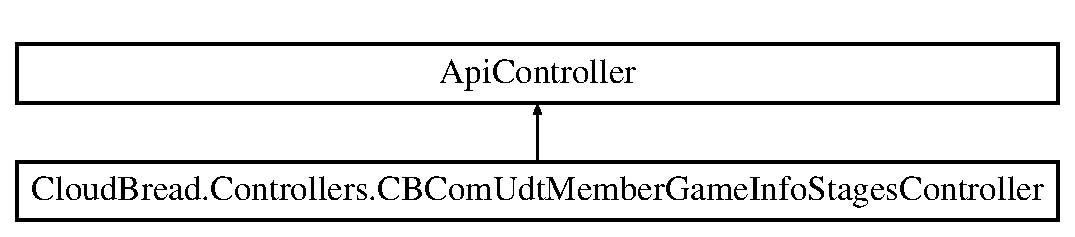
\includegraphics[height=2.000000cm]{a00024}
\end{center}
\end{figure}
\subsection*{Classes}
\begin{DoxyCompactItemize}
\item 
class \hyperlink{a00102}{Input\+Params}
\end{DoxyCompactItemize}
\subsection*{Public Member Functions}
\begin{DoxyCompactItemize}
\item 
string {\bfseries Post} (\hyperlink{a00102}{Input\+Params} p)\hypertarget{a00024_aa1e7d18f4f7835c2f6c81d1972d1481a}{}\label{a00024_aa1e7d18f4f7835c2f6c81d1972d1481a}

\end{DoxyCompactItemize}


The documentation for this class was generated from the following file\+:\begin{DoxyCompactItemize}
\item 
C\+:/\+Users/dwkim/\+Documents/\+Git\+Hub/\+Cloud\+Bread/\+Cloud\+Bread/\+Controllers/\hyperlink{a00199}{C\+B\+Add\+Use\+Member\+Item\+Controller.\+cs}\end{DoxyCompactItemize}

\hypertarget{a00025}{}\section{Cloud\+Bread.\+Controllers.\+C\+B\+Com\+Udt\+Member\+Item\+Controller Class Reference}
\label{a00025}\index{Cloud\+Bread.\+Controllers.\+C\+B\+Com\+Udt\+Member\+Item\+Controller@{Cloud\+Bread.\+Controllers.\+C\+B\+Com\+Udt\+Member\+Item\+Controller}}
Inheritance diagram for Cloud\+Bread.\+Controllers.\+C\+B\+Com\+Udt\+Member\+Item\+Controller\+:\begin{figure}[H]
\begin{center}
\leavevmode
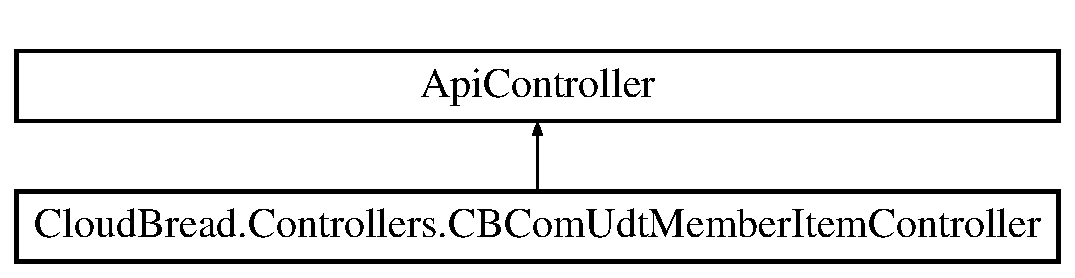
\includegraphics[height=2.000000cm]{a00025}
\end{center}
\end{figure}
\subsection*{Public Member Functions}
\begin{DoxyCompactItemize}
\item 
Http\+Response\+Message \hyperlink{a00025_ad5c9f382ba804a35d3f76b229414d18d}{Post} (\hyperlink{a00072}{Com\+Udt\+Member\+Item\+Input\+Params} p)
\end{DoxyCompactItemize}


\subsection{Member Function Documentation}
\index{Cloud\+Bread\+::\+Controllers\+::\+C\+B\+Com\+Udt\+Member\+Item\+Controller@{Cloud\+Bread\+::\+Controllers\+::\+C\+B\+Com\+Udt\+Member\+Item\+Controller}!Post@{Post}}
\index{Post@{Post}!Cloud\+Bread\+::\+Controllers\+::\+C\+B\+Com\+Udt\+Member\+Item\+Controller@{Cloud\+Bread\+::\+Controllers\+::\+C\+B\+Com\+Udt\+Member\+Item\+Controller}}
\subsubsection[{\texorpdfstring{Post(\+Com\+Udt\+Member\+Item\+Input\+Params p)}{Post(ComUdtMemberItemInputParams p)}}]{\setlength{\rightskip}{0pt plus 5cm}Http\+Response\+Message Cloud\+Bread.\+Controllers.\+C\+B\+Com\+Udt\+Member\+Item\+Controller.\+Post (
\begin{DoxyParamCaption}
\item[{{\bf Com\+Udt\+Member\+Item\+Input\+Params}}]{p}
\end{DoxyParamCaption}
)}\hypertarget{a00025_ad5c9f382ba804a35d3f76b229414d18d}{}\label{a00025_ad5c9f382ba804a35d3f76b229414d18d}
Database connection retry policy

Encrypt the result response 

The documentation for this class was generated from the following file\+:\begin{DoxyCompactItemize}
\item 
C\+:/\+Users/dwkim/\+Documents/\+Git\+Hub/\+Cloud\+Bread/\+Controllers/C\+B\+Com\+Udt\+Member\+Item\+Controller.\+cs\end{DoxyCompactItemize}

\hypertarget{a00026}{}\section{Cloud\+Bread\+Lib.\+D\+A\+L.\+Logger.\+C\+B\+A\+T\+S\+Message\+Entity Class Reference}
\label{a00026}\index{Cloud\+Bread\+Lib.\+D\+A\+L.\+Logger.\+C\+B\+A\+T\+S\+Message\+Entity@{Cloud\+Bread\+Lib.\+D\+A\+L.\+Logger.\+C\+B\+A\+T\+S\+Message\+Entity}}
Inheritance diagram for Cloud\+Bread\+Lib.\+D\+A\+L.\+Logger.\+C\+B\+A\+T\+S\+Message\+Entity\+:\begin{figure}[H]
\begin{center}
\leavevmode
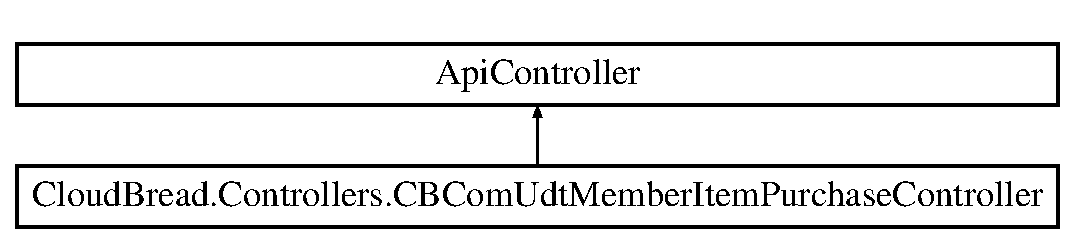
\includegraphics[height=2.000000cm]{a00026}
\end{center}
\end{figure}
\subsection*{Public Member Functions}
\begin{DoxyCompactItemize}
\item 
{\bfseries C\+B\+A\+T\+S\+Message\+Entity} (string pkey, string rkey)\hypertarget{a00026_a5753cc25d529c49183a0b8d089bb4f92}{}\label{a00026_a5753cc25d529c49183a0b8d089bb4f92}

\end{DoxyCompactItemize}
\subsection*{Properties}
\begin{DoxyCompactItemize}
\item 
string {\bfseries D\+B\+Connection\+String}\hspace{0.3cm}{\ttfamily  \mbox{[}get, set\mbox{]}}\hypertarget{a00026_a430054db22907c2f378335b031053a9b}{}\label{a00026_a430054db22907c2f378335b031053a9b}

\item 
string {\bfseries Storage\+Connection\+String}\hspace{0.3cm}{\ttfamily  \mbox{[}get, set\mbox{]}}\hypertarget{a00026_a93feee8e4888958078a0f2231d2deac0}{}\label{a00026_a93feee8e4888958078a0f2231d2deac0}

\item 
string {\bfseries Cloud\+Bread\+Logger\+Setting}\hspace{0.3cm}{\ttfamily  \mbox{[}get, set\mbox{]}}\hypertarget{a00026_ada1533edbb0992304801d639c327118b}{}\label{a00026_ada1533edbb0992304801d639c327118b}

\item 
string {\bfseries Member\+ID}\hspace{0.3cm}{\ttfamily  \mbox{[}get, set\mbox{]}}\hypertarget{a00026_a8eec96d06d55a74e21f23a0cbde3cca4}{}\label{a00026_a8eec96d06d55a74e21f23a0cbde3cca4}

\item 
string {\bfseries job\+ID}\hspace{0.3cm}{\ttfamily  \mbox{[}get, set\mbox{]}}\hypertarget{a00026_a8ece2c804360064b26504c2d1780f8c9}{}\label{a00026_a8ece2c804360064b26504c2d1780f8c9}

\item 
string {\bfseries Date}\hspace{0.3cm}{\ttfamily  \mbox{[}get, set\mbox{]}}\hypertarget{a00026_a4a35cf61f3924278155caf1e80277336}{}\label{a00026_a4a35cf61f3924278155caf1e80277336}

\item 
string {\bfseries Thread}\hspace{0.3cm}{\ttfamily  \mbox{[}get, set\mbox{]}}\hypertarget{a00026_af7db60deee306708cd86edb69acbc86c}{}\label{a00026_af7db60deee306708cd86edb69acbc86c}

\item 
string {\bfseries Level}\hspace{0.3cm}{\ttfamily  \mbox{[}get, set\mbox{]}}\hypertarget{a00026_a3cf1d50a949962f3833142a52cacdd31}{}\label{a00026_a3cf1d50a949962f3833142a52cacdd31}

\item 
string {\bfseries Logger}\hspace{0.3cm}{\ttfamily  \mbox{[}get, set\mbox{]}}\hypertarget{a00026_a0e5a22fa79757a90b6afc8832e6ceffa}{}\label{a00026_a0e5a22fa79757a90b6afc8832e6ceffa}

\item 
string {\bfseries Message}\hspace{0.3cm}{\ttfamily  \mbox{[}get, set\mbox{]}}\hypertarget{a00026_a502ed1378ed622cf1a13a6649ff1afce}{}\label{a00026_a502ed1378ed622cf1a13a6649ff1afce}

\item 
string {\bfseries Exception}\hspace{0.3cm}{\ttfamily  \mbox{[}get, set\mbox{]}}\hypertarget{a00026_a92f31fabac35ccf19e1f9fc8dfb10aee}{}\label{a00026_a92f31fabac35ccf19e1f9fc8dfb10aee}

\end{DoxyCompactItemize}


The documentation for this class was generated from the following file\+:\begin{DoxyCompactItemize}
\item 
C\+:/\+Users/dwkim/\+Documents/\+Git\+Hub/\+Cloud\+Bread/\+Cloud\+Bread\+Lib/\+D\+A\+L/Logger.\+cs\end{DoxyCompactItemize}

\hypertarget{a00027}{}\section{Cloud\+Bread.\+Controllers.\+C\+B\+Ins\+Reg\+Member\+Controller Class Reference}
\label{a00027}\index{Cloud\+Bread.\+Controllers.\+C\+B\+Ins\+Reg\+Member\+Controller@{Cloud\+Bread.\+Controllers.\+C\+B\+Ins\+Reg\+Member\+Controller}}
Inheritance diagram for Cloud\+Bread.\+Controllers.\+C\+B\+Ins\+Reg\+Member\+Controller\+:\begin{figure}[H]
\begin{center}
\leavevmode
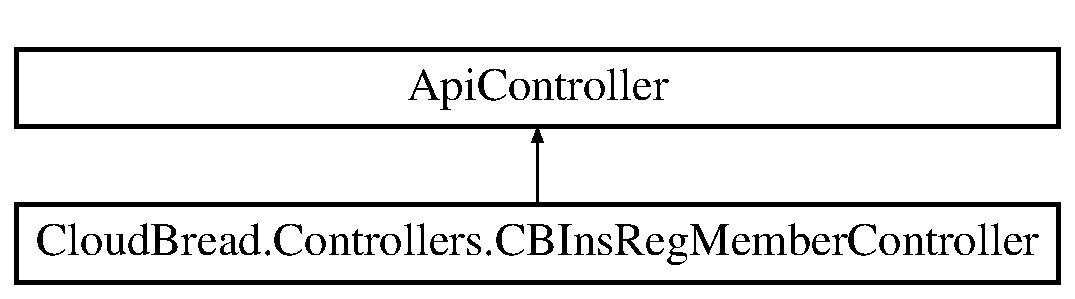
\includegraphics[height=2.000000cm]{a00027}
\end{center}
\end{figure}
\subsection*{Public Member Functions}
\begin{DoxyCompactItemize}
\item 
Http\+Response\+Message \hyperlink{a00027_ad20527b299908589d7d06a8db192b09d}{Post} (\hyperlink{a00077}{Ins\+Reg\+Member\+Input\+Params} p)
\end{DoxyCompactItemize}


\subsection{Member Function Documentation}
\index{Cloud\+Bread\+::\+Controllers\+::\+C\+B\+Ins\+Reg\+Member\+Controller@{Cloud\+Bread\+::\+Controllers\+::\+C\+B\+Ins\+Reg\+Member\+Controller}!Post@{Post}}
\index{Post@{Post}!Cloud\+Bread\+::\+Controllers\+::\+C\+B\+Ins\+Reg\+Member\+Controller@{Cloud\+Bread\+::\+Controllers\+::\+C\+B\+Ins\+Reg\+Member\+Controller}}
\subsubsection[{\texorpdfstring{Post(\+Ins\+Reg\+Member\+Input\+Params p)}{Post(InsRegMemberInputParams p)}}]{\setlength{\rightskip}{0pt plus 5cm}Http\+Response\+Message Cloud\+Bread.\+Controllers.\+C\+B\+Ins\+Reg\+Member\+Controller.\+Post (
\begin{DoxyParamCaption}
\item[{{\bf Ins\+Reg\+Member\+Input\+Params}}]{p}
\end{DoxyParamCaption}
)}\hypertarget{a00027_ad20527b299908589d7d06a8db192b09d}{}\label{a00027_ad20527b299908589d7d06a8db192b09d}
Database connection retry policy

Encrypt the result response 

The documentation for this class was generated from the following file\+:\begin{DoxyCompactItemize}
\item 
C\+:/\+Users/dwkim/\+Documents/\+Git\+Hub/\+Cloud\+Bread/\+Controllers/\hyperlink{a00140}{C\+B\+Ins\+Reg\+Member\+Controller.\+cs}\end{DoxyCompactItemize}

\hypertarget{a00028}{}\section{Cloud\+Bread.\+Controllers.\+C\+B\+Com\+Sel\+Item\+List1\+Controller Class Reference}
\label{a00028}\index{Cloud\+Bread.\+Controllers.\+C\+B\+Com\+Sel\+Item\+List1\+Controller@{Cloud\+Bread.\+Controllers.\+C\+B\+Com\+Sel\+Item\+List1\+Controller}}
Inheritance diagram for Cloud\+Bread.\+Controllers.\+C\+B\+Com\+Sel\+Item\+List1\+Controller\+:\begin{figure}[H]
\begin{center}
\leavevmode
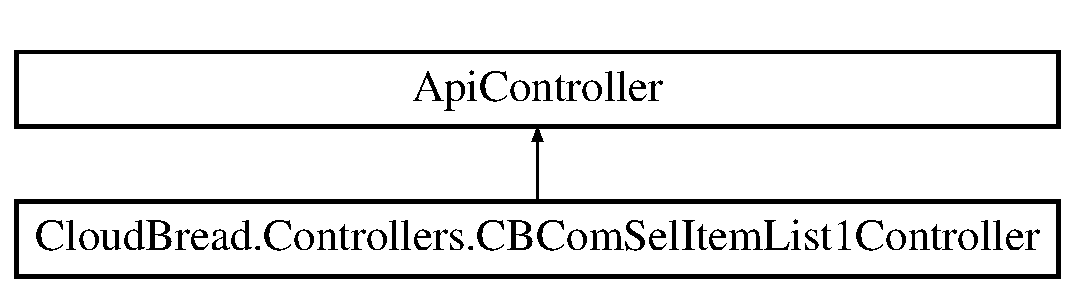
\includegraphics[height=2.000000cm]{a00028}
\end{center}
\end{figure}
\subsection*{Classes}
\begin{DoxyCompactItemize}
\item 
class \hyperlink{a00122}{Input\+Params}
\item 
class \hyperlink{a00149}{Model}
\end{DoxyCompactItemize}
\subsection*{Public Member Functions}
\begin{DoxyCompactItemize}
\item 
List$<$ \hyperlink{a00149}{Model} $>$ {\bfseries Post} (\hyperlink{a00122}{Input\+Params} p)\hypertarget{a00028_af380b95d0be1eecc1e870c9980be4e94}{}\label{a00028_af380b95d0be1eecc1e870c9980be4e94}

\end{DoxyCompactItemize}


The documentation for this class was generated from the following file\+:\begin{DoxyCompactItemize}
\item 
C\+:/\+Users/dwkim/\+Documents/\+Git\+Hub/\+Cloud\+Bread/\+Cloud\+Bread/\+Controllers/\hyperlink{a00201}{C\+B\+Com\+Sel\+Item\+List1\+Controller.\+cs}\end{DoxyCompactItemize}

\hypertarget{a00029}{}\section{Cloud\+Bread.\+Controllers.\+C\+B\+Rank\+Controller Class Reference}
\label{a00029}\index{Cloud\+Bread.\+Controllers.\+C\+B\+Rank\+Controller@{Cloud\+Bread.\+Controllers.\+C\+B\+Rank\+Controller}}
Inheritance diagram for Cloud\+Bread.\+Controllers.\+C\+B\+Rank\+Controller\+:\begin{figure}[H]
\begin{center}
\leavevmode
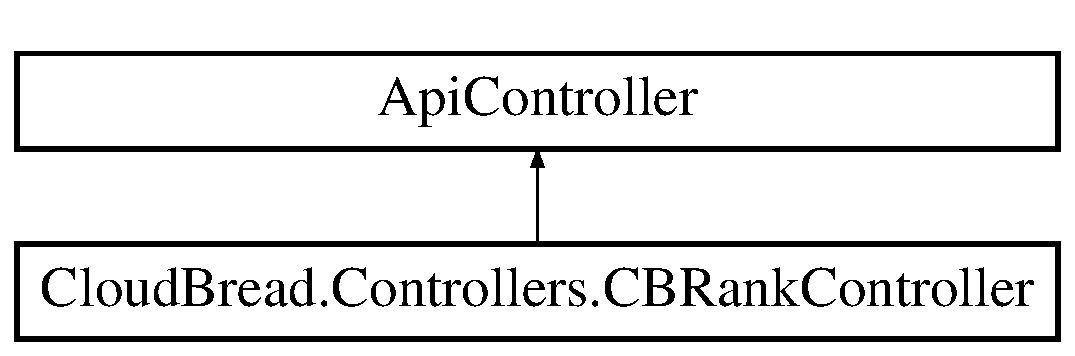
\includegraphics[height=2.000000cm]{a00029}
\end{center}
\end{figure}
\subsection*{Classes}
\begin{DoxyCompactItemize}
\item 
class \hyperlink{a00076}{Input\+Params}
\item 
class \hyperlink{a00079}{Member\+Rank\+Number}
\end{DoxyCompactItemize}
\subsection*{Public Member Functions}
\begin{DoxyCompactItemize}
\item 
\hyperlink{a00079}{Member\+Rank\+Number} \hyperlink{a00029_a5fab62465936cadf09f5f566e327fdba}{Get} (string sid)
\begin{DoxyCompactList}\small\item\em Get member rank order number. \end{DoxyCompactList}\item 
Sorted\+Set\+Entry\mbox{[}$\,$\mbox{]} \hyperlink{a00029_a92ec1412458c02b686672a2cdc031fd6}{G\+ET} (string sid, long start\+Rank, long end\+Rank)
\begin{DoxyCompactList}\small\item\em Get my rank and then call this method to fetch +-\/10 rank(total 20) rank. \end{DoxyCompactList}\item 
Sorted\+Set\+Entry\mbox{[}$\,$\mbox{]} \hyperlink{a00029_a50d3b9e65f0ba0dd87c1db7333842474}{G\+ET} (string sid, int countnum)
\begin{DoxyCompactList}\small\item\em Get top x rankers list order by score desc. \end{DoxyCompactList}\item 
\hyperlink{a00079}{Member\+Rank\+Number} \hyperlink{a00029_a00001336761da0a7c12b8acca93bd69b}{P\+O\+ST} (\hyperlink{a00076}{Input\+Params} p)
\begin{DoxyCompactList}\small\item\em Set redis rank by member. \end{DoxyCompactList}\end{DoxyCompactItemize}


\subsection{Member Function Documentation}
\index{Cloud\+Bread\+::\+Controllers\+::\+C\+B\+Rank\+Controller@{Cloud\+Bread\+::\+Controllers\+::\+C\+B\+Rank\+Controller}!Get@{Get}}
\index{Get@{Get}!Cloud\+Bread\+::\+Controllers\+::\+C\+B\+Rank\+Controller@{Cloud\+Bread\+::\+Controllers\+::\+C\+B\+Rank\+Controller}}
\subsubsection[{\texorpdfstring{Get(string sid)}{Get(string sid)}}]{\setlength{\rightskip}{0pt plus 5cm}{\bf Member\+Rank\+Number} Cloud\+Bread.\+Controllers.\+C\+B\+Rank\+Controller.\+Get (
\begin{DoxyParamCaption}
\item[{string}]{sid}
\end{DoxyParamCaption}
)}\hypertarget{a00029_a5fab62465936cadf09f5f566e327fdba}{}\label{a00029_a5fab62465936cadf09f5f566e327fdba}


Get member rank order number. 

logging purpose

fetch redis value by member sid \index{Cloud\+Bread\+::\+Controllers\+::\+C\+B\+Rank\+Controller@{Cloud\+Bread\+::\+Controllers\+::\+C\+B\+Rank\+Controller}!G\+ET@{G\+ET}}
\index{G\+ET@{G\+ET}!Cloud\+Bread\+::\+Controllers\+::\+C\+B\+Rank\+Controller@{Cloud\+Bread\+::\+Controllers\+::\+C\+B\+Rank\+Controller}}
\subsubsection[{\texorpdfstring{G\+E\+T(string sid, long start\+Rank, long end\+Rank)}{GET(string sid, long startRank, long endRank)}}]{\setlength{\rightskip}{0pt plus 5cm}Sorted\+Set\+Entry \mbox{[}$\,$\mbox{]} Cloud\+Bread.\+Controllers.\+C\+B\+Rank\+Controller.\+G\+ET (
\begin{DoxyParamCaption}
\item[{string}]{sid, }
\item[{long}]{start\+Rank, }
\item[{long}]{end\+Rank}
\end{DoxyParamCaption}
)}\hypertarget{a00029_a92ec1412458c02b686672a2cdc031fd6}{}\label{a00029_a92ec1412458c02b686672a2cdc031fd6}


Get my rank and then call this method to fetch +-\/10 rank(total 20) rank. 

\begin{DoxyRefDesc}{Todo}
\item[\hyperlink{a00001__todo000010}{Todo}]not a good idea getting sid from usermode \end{DoxyRefDesc}
logging purpose

fetch redis list by rank range \index{Cloud\+Bread\+::\+Controllers\+::\+C\+B\+Rank\+Controller@{Cloud\+Bread\+::\+Controllers\+::\+C\+B\+Rank\+Controller}!G\+ET@{G\+ET}}
\index{G\+ET@{G\+ET}!Cloud\+Bread\+::\+Controllers\+::\+C\+B\+Rank\+Controller@{Cloud\+Bread\+::\+Controllers\+::\+C\+B\+Rank\+Controller}}
\subsubsection[{\texorpdfstring{G\+E\+T(string sid, int countnum)}{GET(string sid, int countnum)}}]{\setlength{\rightskip}{0pt plus 5cm}Sorted\+Set\+Entry \mbox{[}$\,$\mbox{]} Cloud\+Bread.\+Controllers.\+C\+B\+Rank\+Controller.\+G\+ET (
\begin{DoxyParamCaption}
\item[{string}]{sid, }
\item[{int}]{countnum}
\end{DoxyParamCaption}
)}\hypertarget{a00029_a50d3b9e65f0ba0dd87c1db7333842474}{}\label{a00029_a50d3b9e65f0ba0dd87c1db7333842474}


Get top x rankers list order by score desc. 

logging purpose

fetch redis list by top countnum rankers \index{Cloud\+Bread\+::\+Controllers\+::\+C\+B\+Rank\+Controller@{Cloud\+Bread\+::\+Controllers\+::\+C\+B\+Rank\+Controller}!P\+O\+ST@{P\+O\+ST}}
\index{P\+O\+ST@{P\+O\+ST}!Cloud\+Bread\+::\+Controllers\+::\+C\+B\+Rank\+Controller@{Cloud\+Bread\+::\+Controllers\+::\+C\+B\+Rank\+Controller}}
\subsubsection[{\texorpdfstring{P\+O\+S\+T(\+Input\+Params p)}{POST(InputParams p)}}]{\setlength{\rightskip}{0pt plus 5cm}{\bf Member\+Rank\+Number} Cloud\+Bread.\+Controllers.\+C\+B\+Rank\+Controller.\+P\+O\+ST (
\begin{DoxyParamCaption}
\item[{{\bf Input\+Params}}]{p}
\end{DoxyParamCaption}
)}\hypertarget{a00029_a00001336761da0a7c12b8acca93bd69b}{}\label{a00029_a00001336761da0a7c12b8acca93bd69b}


Set redis rank by member. 

logging purpose

set redis point and return 

The documentation for this class was generated from the following file\+:\begin{DoxyCompactItemize}
\item 
C\+:/\+Users/dwkim/\+Documents/\+Git\+Hub/\+Cloud\+Bread/\+Controllers/C\+B\+Rank\+Controller.\+cs\end{DoxyCompactItemize}

\hypertarget{a00030}{}\section{Cloud\+Bread\+Redis.\+C\+B\+Redis Class Reference}
\label{a00030}\index{Cloud\+Bread\+Redis.\+C\+B\+Redis@{Cloud\+Bread\+Redis.\+C\+B\+Redis}}
\subsection*{Static Public Member Functions}
\begin{DoxyCompactItemize}
\item 
static bool \hyperlink{a00030_a78e0461fa8abc3fec82245c2595d91ac}{Set\+Redis\+Key} (string key, string value, int?exp\+Time\+Min)\hypertarget{a00030_a78e0461fa8abc3fec82245c2595d91ac}{}\label{a00030_a78e0461fa8abc3fec82245c2595d91ac}

\begin{DoxyCompactList}\small\item\em save socket auth key in redis db0 \end{DoxyCompactList}\item 
static string \hyperlink{a00030_a4339caf935cbbc8ac829cd914f9b3fe9}{Get\+Redis\+Key\+Value} (string key)\hypertarget{a00030_a4339caf935cbbc8ac829cd914f9b3fe9}{}\label{a00030_a4339caf935cbbc8ac829cd914f9b3fe9}

\begin{DoxyCompactList}\small\item\em get socket auth key redis data by key value \end{DoxyCompactList}\item 
static bool \hyperlink{a00030_ab09bc8445fb690da0cdcf9a4983906ed}{Set\+Sorted\+Set\+Rank} (string sid, double point)\hypertarget{a00030_ab09bc8445fb690da0cdcf9a4983906ed}{}\label{a00030_ab09bc8445fb690da0cdcf9a4983906ed}

\begin{DoxyCompactList}\small\item\em Set point value at Redis sorted set. \end{DoxyCompactList}\item 
static long \hyperlink{a00030_af36763a72f5679bc432a013f39beb944}{Get\+Sorted\+Set\+Rank} (string sid)\hypertarget{a00030_af36763a72f5679bc432a013f39beb944}{}\label{a00030_af36763a72f5679bc432a013f39beb944}

\begin{DoxyCompactList}\small\item\em Get rank value from Redis sorted set. \end{DoxyCompactList}\item 
static Sorted\+Set\+Entry\mbox{[}$\,$\mbox{]} \hyperlink{a00030_aa3a4020436145c6f99d2b6f5cc5a5056}{Get\+Sorted\+Set\+Rank\+By\+Range} (long start\+Rank, long end\+Rank)\hypertarget{a00030_aa3a4020436145c6f99d2b6f5cc5a5056}{}\label{a00030_aa3a4020436145c6f99d2b6f5cc5a5056}

\begin{DoxyCompactList}\small\item\em Get selected rank range members. Get my rank and then call this method to fetch +-\/10 rank(total 20) rank. \end{DoxyCompactList}\item 
static Sorted\+Set\+Entry\mbox{[}$\,$\mbox{]} \hyperlink{a00030_a66d68dc112b34f47141bfcac4bf743ea}{Get\+Top\+Sorted\+Set\+Rank} (int count\+Number)\hypertarget{a00030_a66d68dc112b34f47141bfcac4bf743ea}{}\label{a00030_a66d68dc112b34f47141bfcac4bf743ea}

\begin{DoxyCompactList}\small\item\em Get top rank point and info from Redis sorted set. \end{DoxyCompactList}\item 
static bool \hyperlink{a00030_a8227a017bb2cf72e82c0540aec88f66f}{Fill\+All\+Rank\+From\+DB} ()
\item 
static void \hyperlink{a00030_a5b410be6b427222ca5991bf1ed66d3c4}{save\+Redis\+Log} (string key, string message, int?exp\+Time\+Days)\hypertarget{a00030_a5b410be6b427222ca5991bf1ed66d3c4}{}\label{a00030_a5b410be6b427222ca5991bf1ed66d3c4}

\begin{DoxyCompactList}\small\item\em save log to redis db2 and keep 365 days \end{DoxyCompactList}\end{DoxyCompactItemize}


\subsection{Member Function Documentation}
\index{Cloud\+Bread\+Redis\+::\+C\+B\+Redis@{Cloud\+Bread\+Redis\+::\+C\+B\+Redis}!Fill\+All\+Rank\+From\+DB@{Fill\+All\+Rank\+From\+DB}}
\index{Fill\+All\+Rank\+From\+DB@{Fill\+All\+Rank\+From\+DB}!Cloud\+Bread\+Redis\+::\+C\+B\+Redis@{Cloud\+Bread\+Redis\+::\+C\+B\+Redis}}
\subsubsection[{\texorpdfstring{Fill\+All\+Rank\+From\+D\+B()}{FillAllRankFromDB()}}]{\setlength{\rightskip}{0pt plus 5cm}static bool Cloud\+Bread\+Redis.\+C\+B\+Redis.\+Fill\+All\+Rank\+From\+DB (
\begin{DoxyParamCaption}
{}
\end{DoxyParamCaption}
)\hspace{0.3cm}{\ttfamily [static]}}\hypertarget{a00030_a8227a017bb2cf72e82c0540aec88f66f}{}\label{a00030_a8227a017bb2cf72e82c0540aec88f66f}
fill out all rank redis cache from db \begin{DoxyRefDesc}{Todo}
\item[\hyperlink{a00001__todo000002}{Todo}]\+: huge amount of data processing -\/ split 10,000 or ... dt.\+Rows check. if bigger than 10,000, seperate as another loop dt.\+Rows / 10,000 = mod value + 1 = loop count........... call count query first and then paging processing at query side to prevent DB throttling? \end{DoxyRefDesc}
make Sorted\+Set\+Entry to fill out 

The documentation for this class was generated from the following file\+:\begin{DoxyCompactItemize}
\item 
C\+:/\+Users/dwkim/\+Documents/\+Git\+Hub/\+Cloud\+Bread/\hyperlink{a00118}{C\+B\+Redis.\+cs}\end{DoxyCompactItemize}

\hypertarget{a00031}{}\section{Cloud\+Bread.\+Controllers.\+C\+B\+Sel\+Game\+Events\+Controller Class Reference}
\label{a00031}\index{Cloud\+Bread.\+Controllers.\+C\+B\+Sel\+Game\+Events\+Controller@{Cloud\+Bread.\+Controllers.\+C\+B\+Sel\+Game\+Events\+Controller}}
Inheritance diagram for Cloud\+Bread.\+Controllers.\+C\+B\+Sel\+Game\+Events\+Controller\+:\begin{figure}[H]
\begin{center}
\leavevmode
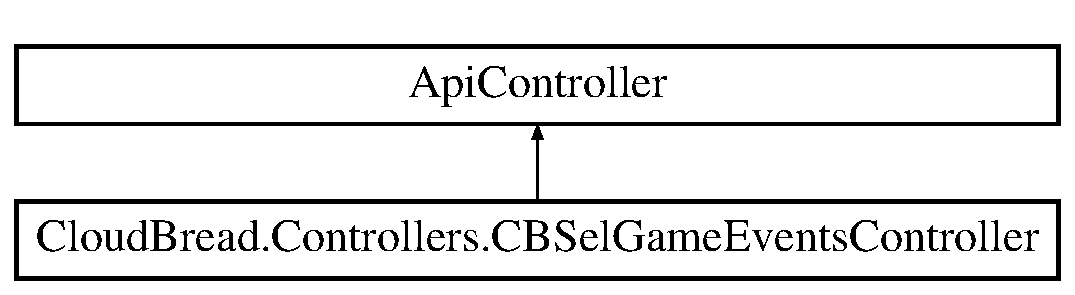
\includegraphics[height=2.000000cm]{a00031}
\end{center}
\end{figure}
\subsection*{Public Member Functions}
\begin{DoxyCompactItemize}
\item 
Http\+Response\+Message \hyperlink{a00031_aca6a9ce203ca57b78a80f3bca3a22fd3}{Post} (\hyperlink{a00086}{Sel\+Game\+Events\+Input\+Params} p)
\end{DoxyCompactItemize}


\subsection{Member Function Documentation}
\index{Cloud\+Bread\+::\+Controllers\+::\+C\+B\+Sel\+Game\+Events\+Controller@{Cloud\+Bread\+::\+Controllers\+::\+C\+B\+Sel\+Game\+Events\+Controller}!Post@{Post}}
\index{Post@{Post}!Cloud\+Bread\+::\+Controllers\+::\+C\+B\+Sel\+Game\+Events\+Controller@{Cloud\+Bread\+::\+Controllers\+::\+C\+B\+Sel\+Game\+Events\+Controller}}
\subsubsection[{\texorpdfstring{Post(\+Sel\+Game\+Events\+Input\+Params p)}{Post(SelGameEventsInputParams p)}}]{\setlength{\rightskip}{0pt plus 5cm}Http\+Response\+Message Cloud\+Bread.\+Controllers.\+C\+B\+Sel\+Game\+Events\+Controller.\+Post (
\begin{DoxyParamCaption}
\item[{{\bf Sel\+Game\+Events\+Input\+Params}}]{p}
\end{DoxyParamCaption}
)}\hypertarget{a00031_aca6a9ce203ca57b78a80f3bca3a22fd3}{}\label{a00031_aca6a9ce203ca57b78a80f3bca3a22fd3}
Database connection retry policy

Encrypt the result response 

The documentation for this class was generated from the following file\+:\begin{DoxyCompactItemize}
\item 
C\+:/\+Users/dwkim/\+Documents/\+Git\+Hub/\+Cloud\+Bread/\+Controllers/\hyperlink{a00143}{C\+B\+Sel\+Game\+Events\+Controller.\+cs}\end{DoxyCompactItemize}

\hypertarget{a00032}{}\section{Cloud\+Bread.\+Controllers.\+C\+B\+Com\+Sel\+Member\+Item\+Controller Class Reference}
\label{a00032}\index{Cloud\+Bread.\+Controllers.\+C\+B\+Com\+Sel\+Member\+Item\+Controller@{Cloud\+Bread.\+Controllers.\+C\+B\+Com\+Sel\+Member\+Item\+Controller}}
Inheritance diagram for Cloud\+Bread.\+Controllers.\+C\+B\+Com\+Sel\+Member\+Item\+Controller\+:\begin{figure}[H]
\begin{center}
\leavevmode
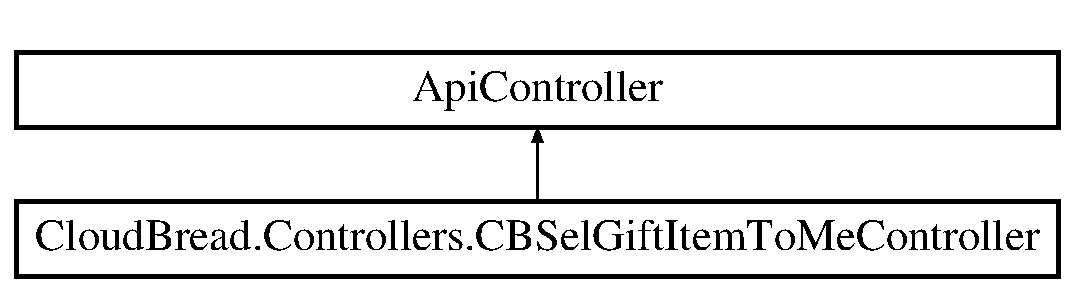
\includegraphics[height=2.000000cm]{a00032}
\end{center}
\end{figure}
\subsection*{Classes}
\begin{DoxyCompactItemize}
\item 
class \hyperlink{a00121}{Input\+Params}
\item 
class \hyperlink{a00159}{Model}
\end{DoxyCompactItemize}
\subsection*{Public Member Functions}
\begin{DoxyCompactItemize}
\item 
List$<$ \hyperlink{a00159}{Model} $>$ {\bfseries Post} (\hyperlink{a00121}{Input\+Params} p)\hypertarget{a00032_aea063fa18a972ddbe9741f3c1d17af63}{}\label{a00032_aea063fa18a972ddbe9741f3c1d17af63}

\end{DoxyCompactItemize}


The documentation for this class was generated from the following file\+:\begin{DoxyCompactItemize}
\item 
C\+:/\+Users/dwkim/\+Documents/\+Git\+Hub/\+Cloud\+Bread/\+Cloud\+Bread/\+Controllers/\hyperlink{a00205}{C\+B\+Com\+Sel\+Member\+Item\+Controller.\+cs}\end{DoxyCompactItemize}

\hypertarget{a00033}{}\section{Cloud\+Bread.\+Controllers.\+C\+B\+Com\+Sel\+Member\+Item\+Purchase\+Controller Class Reference}
\label{a00033}\index{Cloud\+Bread.\+Controllers.\+C\+B\+Com\+Sel\+Member\+Item\+Purchase\+Controller@{Cloud\+Bread.\+Controllers.\+C\+B\+Com\+Sel\+Member\+Item\+Purchase\+Controller}}
Inheritance diagram for Cloud\+Bread.\+Controllers.\+C\+B\+Com\+Sel\+Member\+Item\+Purchase\+Controller\+:\begin{figure}[H]
\begin{center}
\leavevmode
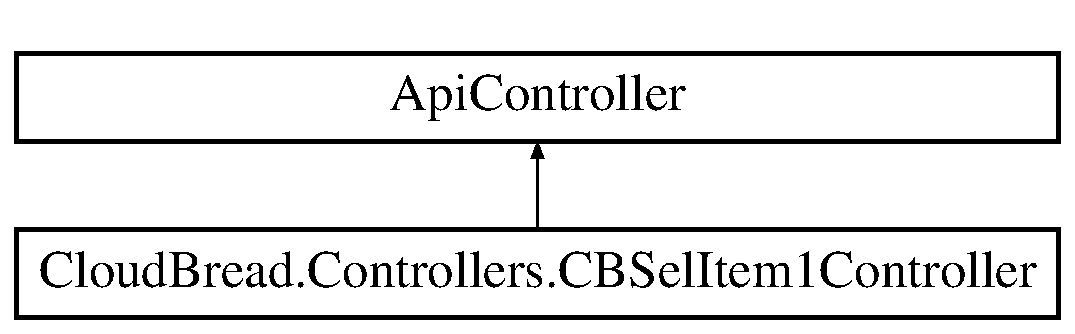
\includegraphics[height=2.000000cm]{a00033}
\end{center}
\end{figure}
\subsection*{Classes}
\begin{DoxyCompactItemize}
\item 
class \hyperlink{a00123}{Input\+Params}
\item 
class \hyperlink{a00153}{Model}
\end{DoxyCompactItemize}
\subsection*{Public Member Functions}
\begin{DoxyCompactItemize}
\item 
List$<$ \hyperlink{a00153}{Model} $>$ {\bfseries Post} (\hyperlink{a00123}{Input\+Params} p)\hypertarget{a00033_a465f776801d7078ce72ee87ebb05992b}{}\label{a00033_a465f776801d7078ce72ee87ebb05992b}

\end{DoxyCompactItemize}


The documentation for this class was generated from the following file\+:\begin{DoxyCompactItemize}
\item 
C\+:/\+Users/dwkim/\+Documents/\+Git\+Hub/\+Cloud\+Bread/\+Cloud\+Bread/\+Controllers/\hyperlink{a00206}{C\+B\+Com\+Sel\+Member\+Item\+Purchase\+Controller.\+cs}\end{DoxyCompactItemize}

\hypertarget{a00034}{}\section{Cloud\+Bread.\+Controllers.\+C\+B\+Com\+Udt\+Gift\+Depository\+Controller Class Reference}
\label{a00034}\index{Cloud\+Bread.\+Controllers.\+C\+B\+Com\+Udt\+Gift\+Depository\+Controller@{Cloud\+Bread.\+Controllers.\+C\+B\+Com\+Udt\+Gift\+Depository\+Controller}}
Inheritance diagram for Cloud\+Bread.\+Controllers.\+C\+B\+Com\+Udt\+Gift\+Depository\+Controller\+:\begin{figure}[H]
\begin{center}
\leavevmode
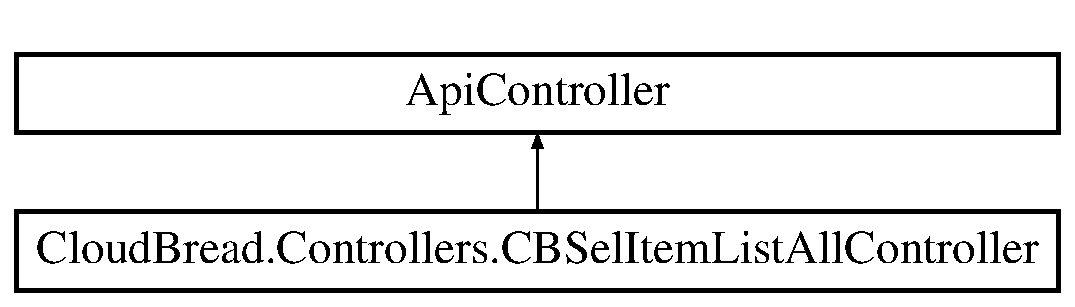
\includegraphics[height=2.000000cm]{a00034}
\end{center}
\end{figure}
\subsection*{Classes}
\begin{DoxyCompactItemize}
\item 
class \hyperlink{a00092}{Input\+Params}
\end{DoxyCompactItemize}
\subsection*{Public Member Functions}
\begin{DoxyCompactItemize}
\item 
string {\bfseries Post} (\hyperlink{a00092}{Input\+Params} p)\hypertarget{a00034_a0ae6cc00b730b70f9ed6c5541f1bcc96}{}\label{a00034_a0ae6cc00b730b70f9ed6c5541f1bcc96}

\end{DoxyCompactItemize}


The documentation for this class was generated from the following file\+:\begin{DoxyCompactItemize}
\item 
C\+:/\+Users/dwkim/\+Documents/\+Git\+Hub/\+Cloud\+Bread/\+Cloud\+Bread/\+Controllers/C\+B\+Com\+Udt\+Gift\+Depository\+Controller.\+cs\end{DoxyCompactItemize}

\hypertarget{a00035}{}\section{Cloud\+Bread.\+Controllers.\+C\+B\+Com\+Udt\+Item\+List1\+Controller Class Reference}
\label{a00035}\index{Cloud\+Bread.\+Controllers.\+C\+B\+Com\+Udt\+Item\+List1\+Controller@{Cloud\+Bread.\+Controllers.\+C\+B\+Com\+Udt\+Item\+List1\+Controller}}
Inheritance diagram for Cloud\+Bread.\+Controllers.\+C\+B\+Com\+Udt\+Item\+List1\+Controller\+:\begin{figure}[H]
\begin{center}
\leavevmode
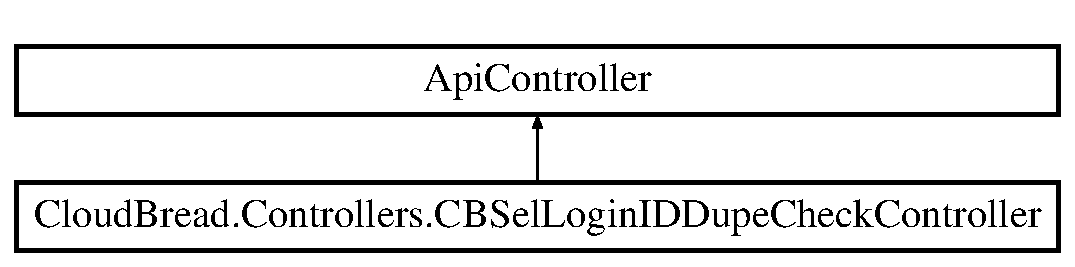
\includegraphics[height=2.000000cm]{a00035}
\end{center}
\end{figure}
\subsection*{Classes}
\begin{DoxyCompactItemize}
\item 
class \hyperlink{a00094}{Input\+Params}
\end{DoxyCompactItemize}
\subsection*{Public Member Functions}
\begin{DoxyCompactItemize}
\item 
string {\bfseries Post} (\hyperlink{a00094}{Input\+Params} p)\hypertarget{a00035_a7acb4a9373b37377aff95ce255e6a694}{}\label{a00035_a7acb4a9373b37377aff95ce255e6a694}

\end{DoxyCompactItemize}


The documentation for this class was generated from the following file\+:\begin{DoxyCompactItemize}
\item 
C\+:/\+Users/dwkim/\+Documents/\+Git\+Hub/\+Cloud\+Bread/\+Cloud\+Bread/\+Controllers/\hyperlink{a00208}{C\+B\+Com\+Udt\+Item\+List1\+Controller.\+cs}\end{DoxyCompactItemize}

\hypertarget{a00036}{}\section{Cloud\+Bread.\+Controllers.\+C\+B\+Sel\+Login\+Info\+Controller Class Reference}
\label{a00036}\index{Cloud\+Bread.\+Controllers.\+C\+B\+Sel\+Login\+Info\+Controller@{Cloud\+Bread.\+Controllers.\+C\+B\+Sel\+Login\+Info\+Controller}}
Inheritance diagram for Cloud\+Bread.\+Controllers.\+C\+B\+Sel\+Login\+Info\+Controller\+:\begin{figure}[H]
\begin{center}
\leavevmode
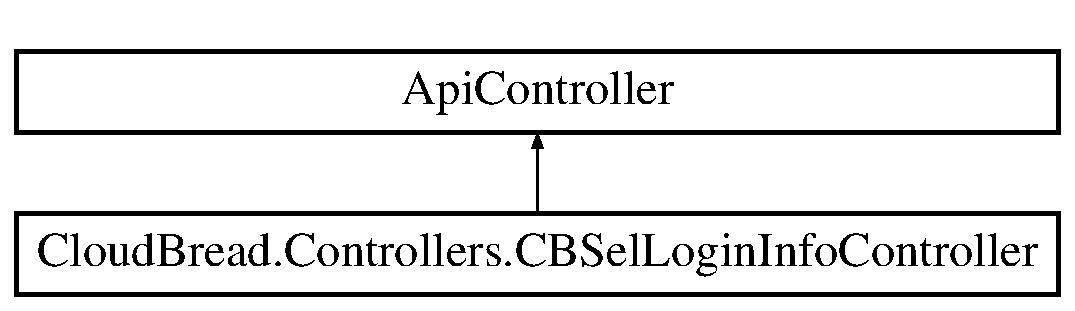
\includegraphics[height=2.000000cm]{a00036}
\end{center}
\end{figure}
\subsection*{Public Member Functions}
\begin{DoxyCompactItemize}
\item 
Http\+Response\+Message \hyperlink{a00036_a87189e37bf8946f77046f9225c75d728}{Post} (\hyperlink{a00096}{Sel\+Login\+Info\+Input\+Params} p)
\end{DoxyCompactItemize}


\subsection{Member Function Documentation}
\index{Cloud\+Bread\+::\+Controllers\+::\+C\+B\+Sel\+Login\+Info\+Controller@{Cloud\+Bread\+::\+Controllers\+::\+C\+B\+Sel\+Login\+Info\+Controller}!Post@{Post}}
\index{Post@{Post}!Cloud\+Bread\+::\+Controllers\+::\+C\+B\+Sel\+Login\+Info\+Controller@{Cloud\+Bread\+::\+Controllers\+::\+C\+B\+Sel\+Login\+Info\+Controller}}
\subsubsection[{\texorpdfstring{Post(\+Sel\+Login\+Info\+Input\+Params p)}{Post(SelLoginInfoInputParams p)}}]{\setlength{\rightskip}{0pt plus 5cm}Http\+Response\+Message Cloud\+Bread.\+Controllers.\+C\+B\+Sel\+Login\+Info\+Controller.\+Post (
\begin{DoxyParamCaption}
\item[{{\bf Sel\+Login\+Info\+Input\+Params}}]{p}
\end{DoxyParamCaption}
)}\hypertarget{a00036_a87189e37bf8946f77046f9225c75d728}{}\label{a00036_a87189e37bf8946f77046f9225c75d728}
Database connection retry policy

Encrypt the result response 

The documentation for this class was generated from the following file\+:\begin{DoxyCompactItemize}
\item 
C\+:/\+Users/dwkim/\+Documents/\+Git\+Hub/\+Cloud\+Bread/\+Controllers/\hyperlink{a00148}{C\+B\+Sel\+Login\+Info\+Controller.\+cs}\end{DoxyCompactItemize}

\hypertarget{a00037}{}\section{Cloud\+Bread.\+Controllers.\+C\+B\+Com\+Udt\+Member\+Game\+Infoes\+Controller Class Reference}
\label{a00037}\index{Cloud\+Bread.\+Controllers.\+C\+B\+Com\+Udt\+Member\+Game\+Infoes\+Controller@{Cloud\+Bread.\+Controllers.\+C\+B\+Com\+Udt\+Member\+Game\+Infoes\+Controller}}
Inheritance diagram for Cloud\+Bread.\+Controllers.\+C\+B\+Com\+Udt\+Member\+Game\+Infoes\+Controller\+:\begin{figure}[H]
\begin{center}
\leavevmode
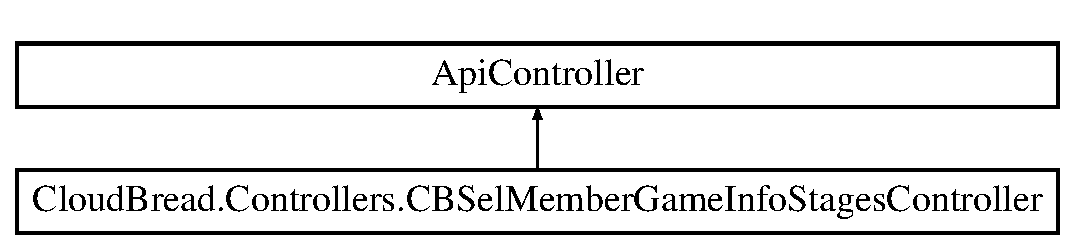
\includegraphics[height=2.000000cm]{a00037}
\end{center}
\end{figure}
\subsection*{Classes}
\begin{DoxyCompactItemize}
\item 
class \hyperlink{a00099}{Input\+Params}
\end{DoxyCompactItemize}
\subsection*{Public Member Functions}
\begin{DoxyCompactItemize}
\item 
string {\bfseries Post} (\hyperlink{a00099}{Input\+Params} p)\hypertarget{a00037_a0de30889beff91cef76eac04ed1acf98}{}\label{a00037_a0de30889beff91cef76eac04ed1acf98}

\end{DoxyCompactItemize}


The documentation for this class was generated from the following file\+:\begin{DoxyCompactItemize}
\item 
C\+:/\+Users/dwkim/\+Documents/\+Git\+Hub/\+Cloud\+Bread/\+Cloud\+Bread/\+Controllers/\hyperlink{a00210}{C\+B\+Com\+Udt\+Member\+Game\+Infoes\+Controller.\+cs}\end{DoxyCompactItemize}

\hypertarget{a00038}{}\section{Cloud\+Bread.\+Controllers.\+C\+B\+Sel\+Member\+Items\+Controller Class Reference}
\label{a00038}\index{Cloud\+Bread.\+Controllers.\+C\+B\+Sel\+Member\+Items\+Controller@{Cloud\+Bread.\+Controllers.\+C\+B\+Sel\+Member\+Items\+Controller}}
Inheritance diagram for Cloud\+Bread.\+Controllers.\+C\+B\+Sel\+Member\+Items\+Controller\+:\begin{figure}[H]
\begin{center}
\leavevmode
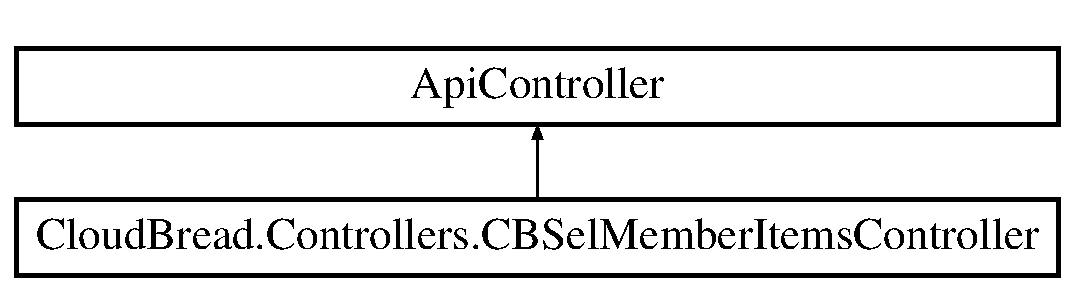
\includegraphics[height=2.000000cm]{a00038}
\end{center}
\end{figure}
\subsection*{Public Member Functions}
\begin{DoxyCompactItemize}
\item 
Http\+Response\+Message \hyperlink{a00038_a4d1793994366b0302d666c7a21bf5932}{Post} (\hyperlink{a00100}{Sel\+Member\+Items\+Input\+Params} p)
\end{DoxyCompactItemize}


\subsection{Member Function Documentation}
\index{Cloud\+Bread\+::\+Controllers\+::\+C\+B\+Sel\+Member\+Items\+Controller@{Cloud\+Bread\+::\+Controllers\+::\+C\+B\+Sel\+Member\+Items\+Controller}!Post@{Post}}
\index{Post@{Post}!Cloud\+Bread\+::\+Controllers\+::\+C\+B\+Sel\+Member\+Items\+Controller@{Cloud\+Bread\+::\+Controllers\+::\+C\+B\+Sel\+Member\+Items\+Controller}}
\subsubsection[{\texorpdfstring{Post(\+Sel\+Member\+Items\+Input\+Params p)}{Post(SelMemberItemsInputParams p)}}]{\setlength{\rightskip}{0pt plus 5cm}Http\+Response\+Message Cloud\+Bread.\+Controllers.\+C\+B\+Sel\+Member\+Items\+Controller.\+Post (
\begin{DoxyParamCaption}
\item[{{\bf Sel\+Member\+Items\+Input\+Params}}]{p}
\end{DoxyParamCaption}
)}\hypertarget{a00038_a4d1793994366b0302d666c7a21bf5932}{}\label{a00038_a4d1793994366b0302d666c7a21bf5932}
Database connection retry policy

Encrypt the result response 

The documentation for this class was generated from the following file\+:\begin{DoxyCompactItemize}
\item 
C\+:/\+Users/dwkim/\+Documents/\+Git\+Hub/\+Cloud\+Bread/\+Controllers/\hyperlink{a00150}{C\+B\+Sel\+Member\+Items\+Controller.\+cs}\end{DoxyCompactItemize}

\hypertarget{a00039}{}\section{Cloud\+Bread.\+Controllers.\+C\+B\+Sel\+Notices\+Controller Class Reference}
\label{a00039}\index{Cloud\+Bread.\+Controllers.\+C\+B\+Sel\+Notices\+Controller@{Cloud\+Bread.\+Controllers.\+C\+B\+Sel\+Notices\+Controller}}
Inheritance diagram for Cloud\+Bread.\+Controllers.\+C\+B\+Sel\+Notices\+Controller\+:\begin{figure}[H]
\begin{center}
\leavevmode
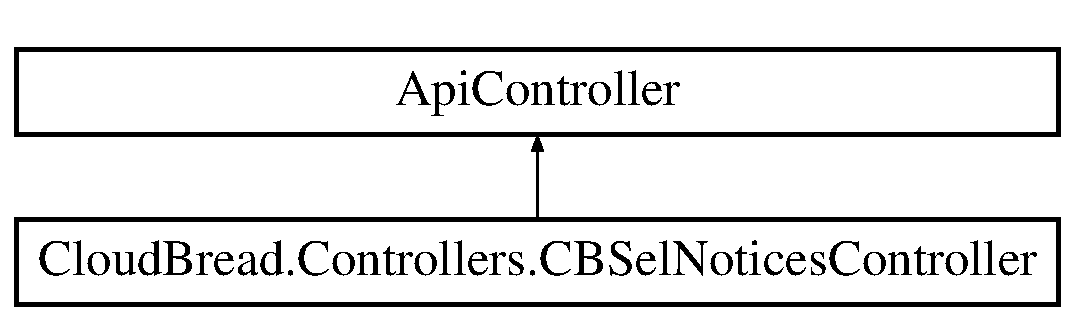
\includegraphics[height=2.000000cm]{a00039}
\end{center}
\end{figure}
\subsection*{Public Member Functions}
\begin{DoxyCompactItemize}
\item 
Http\+Response\+Message \hyperlink{a00039_aa3e4e4704abf851d136970319e92eb46}{Post} (\hyperlink{a00102}{Sel\+Notices\+Input\+Params} p)
\end{DoxyCompactItemize}


\subsection{Member Function Documentation}
\index{Cloud\+Bread\+::\+Controllers\+::\+C\+B\+Sel\+Notices\+Controller@{Cloud\+Bread\+::\+Controllers\+::\+C\+B\+Sel\+Notices\+Controller}!Post@{Post}}
\index{Post@{Post}!Cloud\+Bread\+::\+Controllers\+::\+C\+B\+Sel\+Notices\+Controller@{Cloud\+Bread\+::\+Controllers\+::\+C\+B\+Sel\+Notices\+Controller}}
\subsubsection[{\texorpdfstring{Post(\+Sel\+Notices\+Input\+Params p)}{Post(SelNoticesInputParams p)}}]{\setlength{\rightskip}{0pt plus 5cm}Http\+Response\+Message Cloud\+Bread.\+Controllers.\+C\+B\+Sel\+Notices\+Controller.\+Post (
\begin{DoxyParamCaption}
\item[{{\bf Sel\+Notices\+Input\+Params}}]{p}
\end{DoxyParamCaption}
)}\hypertarget{a00039_aa3e4e4704abf851d136970319e92eb46}{}\label{a00039_aa3e4e4704abf851d136970319e92eb46}
Database connection retry policy

Encrypt the result response 

The documentation for this class was generated from the following file\+:\begin{DoxyCompactItemize}
\item 
C\+:/\+Users/dwkim/\+Documents/\+Git\+Hub/\+Cloud\+Bread/\+Controllers/\hyperlink{a00151}{C\+B\+Sel\+Notices\+Controller.\+cs}\end{DoxyCompactItemize}

\hypertarget{a00040}{}\section{Cloud\+Bread.\+Controllers.\+C\+B\+Sel\+Send\+Email\+To\+Member\+Controller Class Reference}
\label{a00040}\index{Cloud\+Bread.\+Controllers.\+C\+B\+Sel\+Send\+Email\+To\+Member\+Controller@{Cloud\+Bread.\+Controllers.\+C\+B\+Sel\+Send\+Email\+To\+Member\+Controller}}
Inheritance diagram for Cloud\+Bread.\+Controllers.\+C\+B\+Sel\+Send\+Email\+To\+Member\+Controller\+:\begin{figure}[H]
\begin{center}
\leavevmode
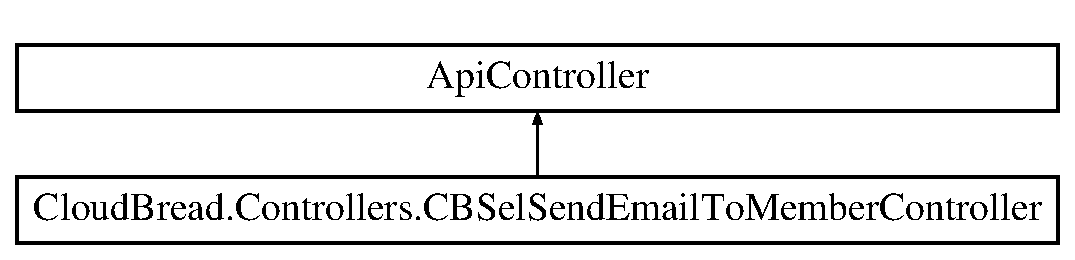
\includegraphics[height=2.000000cm]{a00040}
\end{center}
\end{figure}
\subsection*{Public Member Functions}
\begin{DoxyCompactItemize}
\item 
Http\+Response\+Message \hyperlink{a00040_a0ca95810c4c26811db6f51b9c627c386}{Post} (\hyperlink{a00104}{Sel\+Send\+Email\+To\+Member\+Input\+Params} p)
\end{DoxyCompactItemize}


\subsection{Member Function Documentation}
\index{Cloud\+Bread\+::\+Controllers\+::\+C\+B\+Sel\+Send\+Email\+To\+Member\+Controller@{Cloud\+Bread\+::\+Controllers\+::\+C\+B\+Sel\+Send\+Email\+To\+Member\+Controller}!Post@{Post}}
\index{Post@{Post}!Cloud\+Bread\+::\+Controllers\+::\+C\+B\+Sel\+Send\+Email\+To\+Member\+Controller@{Cloud\+Bread\+::\+Controllers\+::\+C\+B\+Sel\+Send\+Email\+To\+Member\+Controller}}
\subsubsection[{\texorpdfstring{Post(\+Sel\+Send\+Email\+To\+Member\+Input\+Params p)}{Post(SelSendEmailToMemberInputParams p)}}]{\setlength{\rightskip}{0pt plus 5cm}Http\+Response\+Message Cloud\+Bread.\+Controllers.\+C\+B\+Sel\+Send\+Email\+To\+Member\+Controller.\+Post (
\begin{DoxyParamCaption}
\item[{{\bf Sel\+Send\+Email\+To\+Member\+Input\+Params}}]{p}
\end{DoxyParamCaption}
)}\hypertarget{a00040_a0ca95810c4c26811db6f51b9c627c386}{}\label{a00040_a0ca95810c4c26811db6f51b9c627c386}
Database connection retry policy

Encrypt the result response 

The documentation for this class was generated from the following file\+:\begin{DoxyCompactItemize}
\item 
C\+:/\+Users/dwkim/\+Documents/\+Git\+Hub/\+Cloud\+Bread/\+Controllers/\hyperlink{a00152}{C\+B\+Sel\+Send\+Email\+To\+Member\+Controller.\+cs}\end{DoxyCompactItemize}

\hypertarget{a00041}{}\section{Cloud\+Bread.\+Controllers.\+C\+B\+Ins\+Anonymous\+Reg\+Member\+Controller Class Reference}
\label{a00041}\index{Cloud\+Bread.\+Controllers.\+C\+B\+Ins\+Anonymous\+Reg\+Member\+Controller@{Cloud\+Bread.\+Controllers.\+C\+B\+Ins\+Anonymous\+Reg\+Member\+Controller}}
Inheritance diagram for Cloud\+Bread.\+Controllers.\+C\+B\+Ins\+Anonymous\+Reg\+Member\+Controller\+:\begin{figure}[H]
\begin{center}
\leavevmode
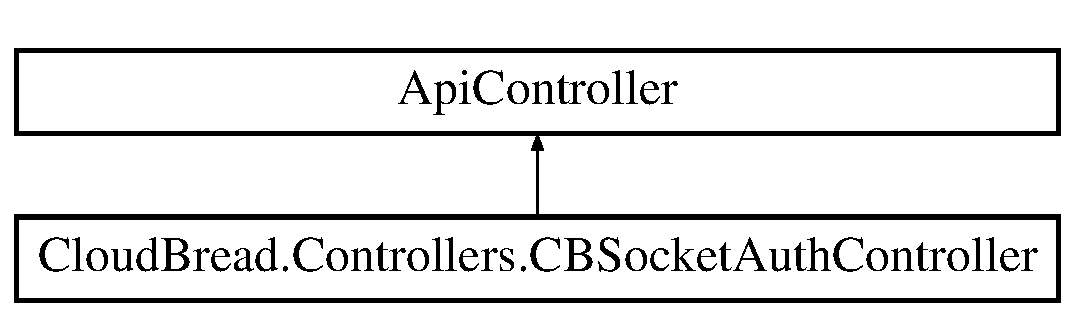
\includegraphics[height=2.000000cm]{a00041}
\end{center}
\end{figure}
\subsection*{Classes}
\begin{DoxyCompactItemize}
\item 
class \hyperlink{a00115}{Input\+Params}
\end{DoxyCompactItemize}
\subsection*{Public Member Functions}
\begin{DoxyCompactItemize}
\item 
string {\bfseries Post} (\hyperlink{a00115}{Input\+Params} p)\hypertarget{a00041_aa0a9dad7adb9084a06daf2dd3dd829b4}{}\label{a00041_aa0a9dad7adb9084a06daf2dd3dd829b4}

\end{DoxyCompactItemize}


The documentation for this class was generated from the following file\+:\begin{DoxyCompactItemize}
\item 
C\+:/\+Users/dwkim/\+Documents/\+Git\+Hub/\+Cloud\+Bread/\+Cloud\+Bread/\+Controllers/\hyperlink{a00214}{C\+B\+Ins\+Anonymous\+Reg\+Member\+Controller.\+cs}\end{DoxyCompactItemize}

\hypertarget{a00042}{}\section{Cloud\+Bread.\+Controllers.\+C\+B\+Socket\+Token\+Valid\+Check\+Controller Class Reference}
\label{a00042}\index{Cloud\+Bread.\+Controllers.\+C\+B\+Socket\+Token\+Valid\+Check\+Controller@{Cloud\+Bread.\+Controllers.\+C\+B\+Socket\+Token\+Valid\+Check\+Controller}}
Inheritance diagram for Cloud\+Bread.\+Controllers.\+C\+B\+Socket\+Token\+Valid\+Check\+Controller\+:\begin{figure}[H]
\begin{center}
\leavevmode
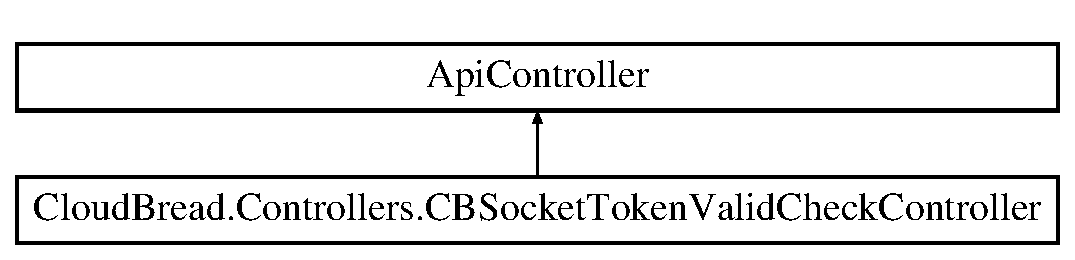
\includegraphics[height=2.000000cm]{a00042}
\end{center}
\end{figure}
\subsection*{Classes}
\begin{DoxyCompactItemize}
\item 
class \hyperlink{a00084}{Result}
\item 
class \hyperlink{a00108}{Token}
\end{DoxyCompactItemize}
\subsection*{Public Member Functions}
\begin{DoxyCompactItemize}
\item 
\hyperlink{a00084}{Result} \hyperlink{a00042_ac02fd3e3889087b81c43c96578e461fc}{P\+O\+ST} (\hyperlink{a00108}{Token} token)
\end{DoxyCompactItemize}


\subsection{Member Function Documentation}
\index{Cloud\+Bread\+::\+Controllers\+::\+C\+B\+Socket\+Token\+Valid\+Check\+Controller@{Cloud\+Bread\+::\+Controllers\+::\+C\+B\+Socket\+Token\+Valid\+Check\+Controller}!P\+O\+ST@{P\+O\+ST}}
\index{P\+O\+ST@{P\+O\+ST}!Cloud\+Bread\+::\+Controllers\+::\+C\+B\+Socket\+Token\+Valid\+Check\+Controller@{Cloud\+Bread\+::\+Controllers\+::\+C\+B\+Socket\+Token\+Valid\+Check\+Controller}}
\subsubsection[{\texorpdfstring{P\+O\+S\+T(\+Token token)}{POST(Token token)}}]{\setlength{\rightskip}{0pt plus 5cm}{\bf Result} Cloud\+Bread.\+Controllers.\+C\+B\+Socket\+Token\+Valid\+Check\+Controller.\+P\+O\+ST (
\begin{DoxyParamCaption}
\item[{{\bf Token}}]{token}
\end{DoxyParamCaption}
)}\hypertarget{a00042_ac02fd3e3889087b81c43c96578e461fc}{}\label{a00042_ac02fd3e3889087b81c43c96578e461fc}
logging purpose

fetch redis value by requested token.\+guid 

The documentation for this class was generated from the following file\+:\begin{DoxyCompactItemize}
\item 
C\+:/\+Users/dwkim/\+Documents/\+Git\+Hub/\+Cloud\+Bread/\+Controllers/C\+B\+Socket\+Token\+Valid\+Check\+Controller.\+cs\end{DoxyCompactItemize}

\hypertarget{a00043}{}\section{Cloud\+Bread.\+Controllers.\+C\+B\+Udt\+Coupon\+Member\+Controller Class Reference}
\label{a00043}\index{Cloud\+Bread.\+Controllers.\+C\+B\+Udt\+Coupon\+Member\+Controller@{Cloud\+Bread.\+Controllers.\+C\+B\+Udt\+Coupon\+Member\+Controller}}
Inheritance diagram for Cloud\+Bread.\+Controllers.\+C\+B\+Udt\+Coupon\+Member\+Controller\+:\begin{figure}[H]
\begin{center}
\leavevmode
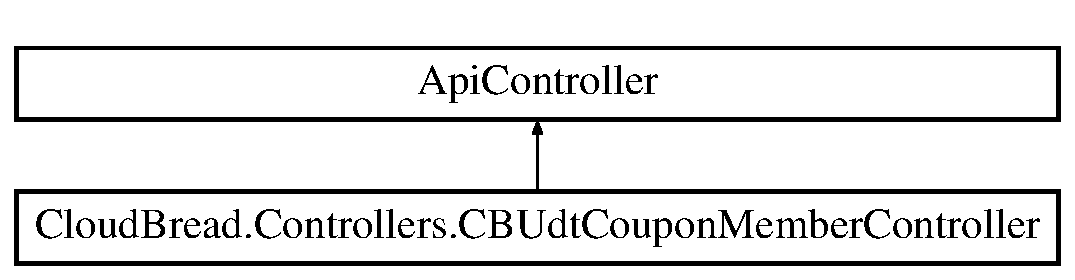
\includegraphics[height=2.000000cm]{a00043}
\end{center}
\end{figure}
\subsection*{Public Member Functions}
\begin{DoxyCompactItemize}
\item 
Http\+Response\+Message \hyperlink{a00043_a816ffd63ecb2323cbedfb21b20c471b2}{Post} (\hyperlink{a00109}{Udt\+Coupon\+Member\+Input\+Params} p)
\end{DoxyCompactItemize}


\subsection{Member Function Documentation}
\index{Cloud\+Bread\+::\+Controllers\+::\+C\+B\+Udt\+Coupon\+Member\+Controller@{Cloud\+Bread\+::\+Controllers\+::\+C\+B\+Udt\+Coupon\+Member\+Controller}!Post@{Post}}
\index{Post@{Post}!Cloud\+Bread\+::\+Controllers\+::\+C\+B\+Udt\+Coupon\+Member\+Controller@{Cloud\+Bread\+::\+Controllers\+::\+C\+B\+Udt\+Coupon\+Member\+Controller}}
\subsubsection[{\texorpdfstring{Post(\+Udt\+Coupon\+Member\+Input\+Params p)}{Post(UdtCouponMemberInputParams p)}}]{\setlength{\rightskip}{0pt plus 5cm}Http\+Response\+Message Cloud\+Bread.\+Controllers.\+C\+B\+Udt\+Coupon\+Member\+Controller.\+Post (
\begin{DoxyParamCaption}
\item[{{\bf Udt\+Coupon\+Member\+Input\+Params}}]{p}
\end{DoxyParamCaption}
)}\hypertarget{a00043_a816ffd63ecb2323cbedfb21b20c471b2}{}\label{a00043_a816ffd63ecb2323cbedfb21b20c471b2}
Database connection retry policy

Encrypt the result response 

The documentation for this class was generated from the following file\+:\begin{DoxyCompactItemize}
\item 
C\+:/\+Users/dwkim/\+Documents/\+Git\+Hub/\+Cloud\+Bread/\+Controllers/\hyperlink{a00156}{C\+B\+Udt\+Coupon\+Member\+Controller.\+cs}\end{DoxyCompactItemize}

\hypertarget{a00044}{}\section{Cloud\+Bread\+Lib.\+D\+A\+L.\+Logger.\+C\+B\+Log\+Message Class Reference}
\label{a00044}\index{Cloud\+Bread\+Lib.\+D\+A\+L.\+Logger.\+C\+B\+Log\+Message@{Cloud\+Bread\+Lib.\+D\+A\+L.\+Logger.\+C\+B\+Log\+Message}}
\subsection*{Properties}
\begin{DoxyCompactItemize}
\item 
string {\bfseries D\+B\+Connection\+String}\hspace{0.3cm}{\ttfamily  \mbox{[}get, set\mbox{]}}\hypertarget{a00044_ae2a4b77a45768901d3b3fb1d9ad56999}{}\label{a00044_ae2a4b77a45768901d3b3fb1d9ad56999}

\item 
string {\bfseries Storage\+Connection\+String}\hspace{0.3cm}{\ttfamily  \mbox{[}get, set\mbox{]}}\hypertarget{a00044_aecdb4b5d752435d17102110ef8d68d60}{}\label{a00044_aecdb4b5d752435d17102110ef8d68d60}

\item 
string {\bfseries Cloud\+Bread\+Logger\+Setting}\hspace{0.3cm}{\ttfamily  \mbox{[}get, set\mbox{]}}\hypertarget{a00044_a27b68a579fcdc11169ba6f051305cc4e}{}\label{a00044_a27b68a579fcdc11169ba6f051305cc4e}

\item 
string {\bfseries member\+ID}\hspace{0.3cm}{\ttfamily  \mbox{[}get, set\mbox{]}}\hypertarget{a00044_ae5b221a36696db8245a90a1d741f2e93}{}\label{a00044_ae5b221a36696db8245a90a1d741f2e93}

\item 
string {\bfseries job\+ID}\hspace{0.3cm}{\ttfamily  \mbox{[}get, set\mbox{]}}\hypertarget{a00044_a06a5091b929c6272fd58ff41c11dc837}{}\label{a00044_a06a5091b929c6272fd58ff41c11dc837}

\item 
string {\bfseries Date}\hspace{0.3cm}{\ttfamily  \mbox{[}get, set\mbox{]}}\hypertarget{a00044_a3e54d4484987301a22735526ef9c5976}{}\label{a00044_a3e54d4484987301a22735526ef9c5976}

\item 
string {\bfseries Thread}\hspace{0.3cm}{\ttfamily  \mbox{[}get, set\mbox{]}}\hypertarget{a00044_aa9adee6a804c6d34a37c6ef47fbfc85e}{}\label{a00044_aa9adee6a804c6d34a37c6ef47fbfc85e}

\item 
string {\bfseries Level}\hspace{0.3cm}{\ttfamily  \mbox{[}get, set\mbox{]}}\hypertarget{a00044_a1d48ff9647c2c2ae0663cc518064fa5f}{}\label{a00044_a1d48ff9647c2c2ae0663cc518064fa5f}

\item 
string {\bfseries Logger}\hspace{0.3cm}{\ttfamily  \mbox{[}get, set\mbox{]}}\hypertarget{a00044_a1985d8f6e35a4092ee08241c932192d7}{}\label{a00044_a1985d8f6e35a4092ee08241c932192d7}

\item 
string {\bfseries Message}\hspace{0.3cm}{\ttfamily  \mbox{[}get, set\mbox{]}}\hypertarget{a00044_a731b50713ec4b57fdaf89572ee8ac35b}{}\label{a00044_a731b50713ec4b57fdaf89572ee8ac35b}

\item 
string {\bfseries Exception}\hspace{0.3cm}{\ttfamily  \mbox{[}get, set\mbox{]}}\hypertarget{a00044_aaa8a8162d82c557946d48b03aa40a959}{}\label{a00044_aaa8a8162d82c557946d48b03aa40a959}

\end{DoxyCompactItemize}


The documentation for this class was generated from the following file\+:\begin{DoxyCompactItemize}
\item 
C\+:/\+Users/dwkim/\+Documents/\+Git\+Hub/\+Cloud\+Bread/\+Cloud\+Bread\+Lib/\+D\+A\+L/Logger.\+cs\end{DoxyCompactItemize}

\hypertarget{a00045}{}\section{Cloud\+Bread.\+Controllers.\+C\+B\+Udt\+Member\+Game\+Info\+Stage\+Controller Class Reference}
\label{a00045}\index{Cloud\+Bread.\+Controllers.\+C\+B\+Udt\+Member\+Game\+Info\+Stage\+Controller@{Cloud\+Bread.\+Controllers.\+C\+B\+Udt\+Member\+Game\+Info\+Stage\+Controller}}
Inheritance diagram for Cloud\+Bread.\+Controllers.\+C\+B\+Udt\+Member\+Game\+Info\+Stage\+Controller\+:\begin{figure}[H]
\begin{center}
\leavevmode
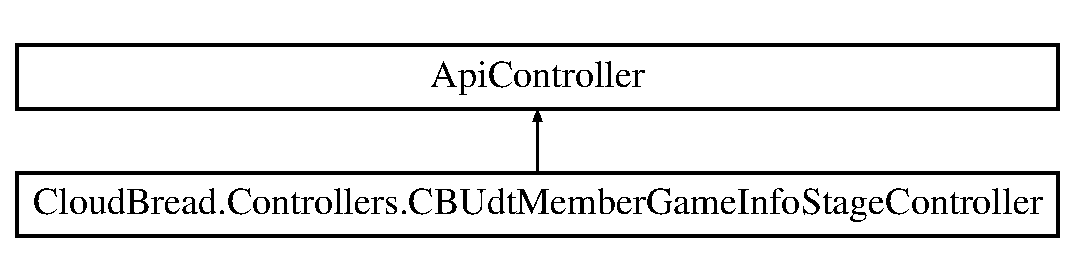
\includegraphics[height=2.000000cm]{a00045}
\end{center}
\end{figure}
\subsection*{Public Member Functions}
\begin{DoxyCompactItemize}
\item 
Http\+Response\+Message \hyperlink{a00045_afd08f989520cbf1e215452bb8901e8e2}{Post} (\hyperlink{a00111}{Udt\+Member\+Game\+Info\+Stage\+Input\+Params} p)
\end{DoxyCompactItemize}


\subsection{Member Function Documentation}
\index{Cloud\+Bread\+::\+Controllers\+::\+C\+B\+Udt\+Member\+Game\+Info\+Stage\+Controller@{Cloud\+Bread\+::\+Controllers\+::\+C\+B\+Udt\+Member\+Game\+Info\+Stage\+Controller}!Post@{Post}}
\index{Post@{Post}!Cloud\+Bread\+::\+Controllers\+::\+C\+B\+Udt\+Member\+Game\+Info\+Stage\+Controller@{Cloud\+Bread\+::\+Controllers\+::\+C\+B\+Udt\+Member\+Game\+Info\+Stage\+Controller}}
\subsubsection[{\texorpdfstring{Post(\+Udt\+Member\+Game\+Info\+Stage\+Input\+Params p)}{Post(UdtMemberGameInfoStageInputParams p)}}]{\setlength{\rightskip}{0pt plus 5cm}Http\+Response\+Message Cloud\+Bread.\+Controllers.\+C\+B\+Udt\+Member\+Game\+Info\+Stage\+Controller.\+Post (
\begin{DoxyParamCaption}
\item[{{\bf Udt\+Member\+Game\+Info\+Stage\+Input\+Params}}]{p}
\end{DoxyParamCaption}
)}\hypertarget{a00045_afd08f989520cbf1e215452bb8901e8e2}{}\label{a00045_afd08f989520cbf1e215452bb8901e8e2}
Database connection retry policy

Encrypt the result response 

The documentation for this class was generated from the following file\+:\begin{DoxyCompactItemize}
\item 
C\+:/\+Users/dwkim/\+Documents/\+Git\+Hub/\+Cloud\+Bread/\+Controllers/\hyperlink{a00158}{C\+B\+Udt\+Member\+Game\+Info\+Stage\+Controller.\+cs}\end{DoxyCompactItemize}

\hypertarget{a00046}{}\section{Cloud\+Bread.\+Controllers.\+C\+B\+Sel\+Game\+Events\+Controller Class Reference}
\label{a00046}\index{Cloud\+Bread.\+Controllers.\+C\+B\+Sel\+Game\+Events\+Controller@{Cloud\+Bread.\+Controllers.\+C\+B\+Sel\+Game\+Events\+Controller}}
Inheritance diagram for Cloud\+Bread.\+Controllers.\+C\+B\+Sel\+Game\+Events\+Controller\+:\begin{figure}[H]
\begin{center}
\leavevmode
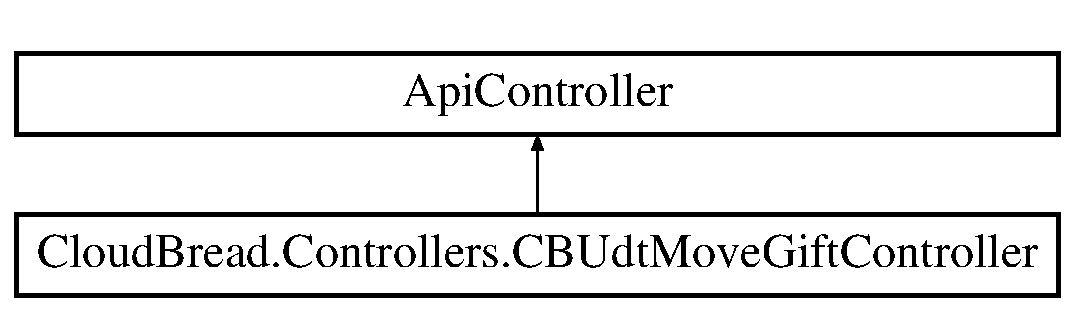
\includegraphics[height=2.000000cm]{a00046}
\end{center}
\end{figure}
\subsection*{Classes}
\begin{DoxyCompactItemize}
\item 
class \hyperlink{a00119}{Input\+Params}
\item 
class \hyperlink{a00166}{Model}
\end{DoxyCompactItemize}
\subsection*{Public Member Functions}
\begin{DoxyCompactItemize}
\item 
List$<$ \hyperlink{a00166}{Model} $>$ {\bfseries Post} (\hyperlink{a00119}{Input\+Params} p)\hypertarget{a00046_a4b7d48b96dfb8d43e274be9d685e824c}{}\label{a00046_a4b7d48b96dfb8d43e274be9d685e824c}

\end{DoxyCompactItemize}


The documentation for this class was generated from the following file\+:\begin{DoxyCompactItemize}
\item 
C\+:/\+Users/dwkim/\+Documents/\+Git\+Hub/\+Cloud\+Bread/\+Cloud\+Bread/\+Controllers/\hyperlink{a00217}{C\+B\+Sel\+Game\+Events\+Controller.\+cs}\end{DoxyCompactItemize}

\hypertarget{a00047}{}\section{Cloud\+Bread.\+Controllers.\+C\+B\+Sel\+Gift\+Item\+To\+Me\+Controller Class Reference}
\label{a00047}\index{Cloud\+Bread.\+Controllers.\+C\+B\+Sel\+Gift\+Item\+To\+Me\+Controller@{Cloud\+Bread.\+Controllers.\+C\+B\+Sel\+Gift\+Item\+To\+Me\+Controller}}
Inheritance diagram for Cloud\+Bread.\+Controllers.\+C\+B\+Sel\+Gift\+Item\+To\+Me\+Controller\+:\begin{figure}[H]
\begin{center}
\leavevmode
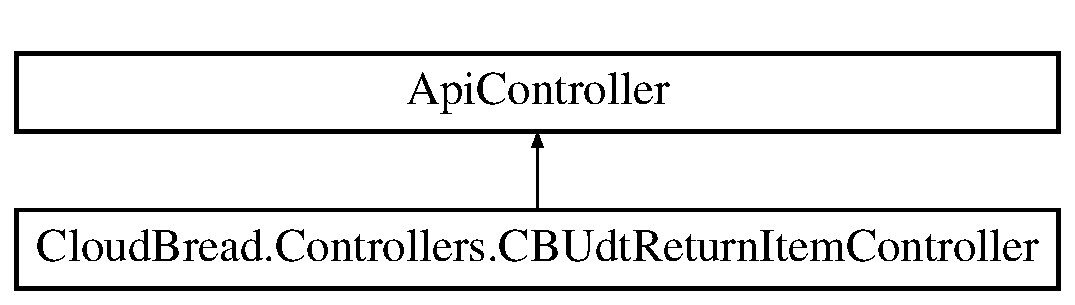
\includegraphics[height=2.000000cm]{a00047}
\end{center}
\end{figure}
\subsection*{Classes}
\begin{DoxyCompactItemize}
\item 
class \hyperlink{a00110}{Input\+Params}
\item 
class \hyperlink{a00151}{Model}
\end{DoxyCompactItemize}
\subsection*{Public Member Functions}
\begin{DoxyCompactItemize}
\item 
List$<$ \hyperlink{a00151}{Model} $>$ {\bfseries Post} (\hyperlink{a00110}{Input\+Params} p)\hypertarget{a00047_a3cb5109a3d17222ee654657916ccf126}{}\label{a00047_a3cb5109a3d17222ee654657916ccf126}

\end{DoxyCompactItemize}


The documentation for this class was generated from the following file\+:\begin{DoxyCompactItemize}
\item 
C\+:/\+Users/dwkim/\+Documents/\+Git\+Hub/\+Cloud\+Bread/\+Cloud\+Bread/\+Controllers/\hyperlink{a00218}{C\+B\+Sel\+Gift\+Item\+To\+Me\+Controller.\+cs}\end{DoxyCompactItemize}

\hypertarget{a00048}{}\section{Cloud\+Bread.\+Controllers.\+C\+B\+Udt\+Send\+Gift\+Controller Class Reference}
\label{a00048}\index{Cloud\+Bread.\+Controllers.\+C\+B\+Udt\+Send\+Gift\+Controller@{Cloud\+Bread.\+Controllers.\+C\+B\+Udt\+Send\+Gift\+Controller}}
Inheritance diagram for Cloud\+Bread.\+Controllers.\+C\+B\+Udt\+Send\+Gift\+Controller\+:\begin{figure}[H]
\begin{center}
\leavevmode
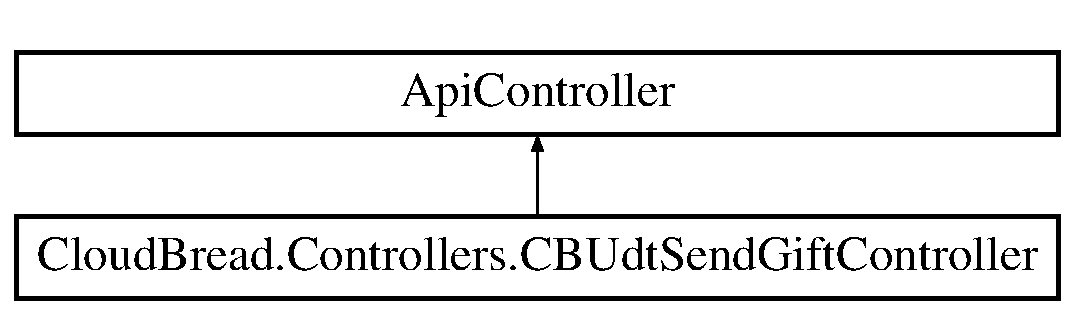
\includegraphics[height=2.000000cm]{a00048}
\end{center}
\end{figure}
\subsection*{Public Member Functions}
\begin{DoxyCompactItemize}
\item 
Http\+Response\+Message \hyperlink{a00048_a2e45836d6b5d569f82388bbd9cf368bd}{Post} (\hyperlink{a00114}{Udt\+Send\+Gift\+Input\+Params} p)
\end{DoxyCompactItemize}


\subsection{Member Function Documentation}
\index{Cloud\+Bread\+::\+Controllers\+::\+C\+B\+Udt\+Send\+Gift\+Controller@{Cloud\+Bread\+::\+Controllers\+::\+C\+B\+Udt\+Send\+Gift\+Controller}!Post@{Post}}
\index{Post@{Post}!Cloud\+Bread\+::\+Controllers\+::\+C\+B\+Udt\+Send\+Gift\+Controller@{Cloud\+Bread\+::\+Controllers\+::\+C\+B\+Udt\+Send\+Gift\+Controller}}
\subsubsection[{\texorpdfstring{Post(\+Udt\+Send\+Gift\+Input\+Params p)}{Post(UdtSendGiftInputParams p)}}]{\setlength{\rightskip}{0pt plus 5cm}Http\+Response\+Message Cloud\+Bread.\+Controllers.\+C\+B\+Udt\+Send\+Gift\+Controller.\+Post (
\begin{DoxyParamCaption}
\item[{{\bf Udt\+Send\+Gift\+Input\+Params}}]{p}
\end{DoxyParamCaption}
)}\hypertarget{a00048_a2e45836d6b5d569f82388bbd9cf368bd}{}\label{a00048_a2e45836d6b5d569f82388bbd9cf368bd}
Database connection retry policy

Encrypt the result response 

The documentation for this class was generated from the following file\+:\begin{DoxyCompactItemize}
\item 
C\+:/\+Users/dwkim/\+Documents/\+Git\+Hub/\+Cloud\+Bread/\+Controllers/\hyperlink{a00162}{C\+B\+Udt\+Send\+Gift\+Controller.\+cs}\end{DoxyCompactItemize}

\hypertarget{a00049}{}\section{Cloud\+Bread.\+Models.\+Com\+Ins\+Member\+Game\+Info\+Stages\+Input\+Params Class Reference}
\label{a00049}\index{Cloud\+Bread.\+Models.\+Com\+Ins\+Member\+Game\+Info\+Stages\+Input\+Params@{Cloud\+Bread.\+Models.\+Com\+Ins\+Member\+Game\+Info\+Stages\+Input\+Params}}
\subsection*{Properties}
\begin{DoxyCompactItemize}
\item 
string {\bfseries Member\+Game\+Info\+Stage\+ID}\hspace{0.3cm}{\ttfamily  \mbox{[}get, set\mbox{]}}\hypertarget{a00049_a5ea1150273c769d9533d51258e30c461}{}\label{a00049_a5ea1150273c769d9533d51258e30c461}

\item 
string {\bfseries Member\+ID}\hspace{0.3cm}{\ttfamily  \mbox{[}get, set\mbox{]}}\hypertarget{a00049_a7770edc46f030003470b81f465df747d}{}\label{a00049_a7770edc46f030003470b81f465df747d}

\item 
string {\bfseries Stage\+Name}\hspace{0.3cm}{\ttfamily  \mbox{[}get, set\mbox{]}}\hypertarget{a00049_a30c614df7f420724e40559c77c5c9c82}{}\label{a00049_a30c614df7f420724e40559c77c5c9c82}

\item 
string {\bfseries Stage\+Status}\hspace{0.3cm}{\ttfamily  \mbox{[}get, set\mbox{]}}\hypertarget{a00049_aec175115a74e99273848c062995dc3d7}{}\label{a00049_aec175115a74e99273848c062995dc3d7}

\item 
string {\bfseries Category1}\hspace{0.3cm}{\ttfamily  \mbox{[}get, set\mbox{]}}\hypertarget{a00049_a541aa1b74364eb30b0cc5e0fb7c9ec43}{}\label{a00049_a541aa1b74364eb30b0cc5e0fb7c9ec43}

\item 
string {\bfseries Category2}\hspace{0.3cm}{\ttfamily  \mbox{[}get, set\mbox{]}}\hypertarget{a00049_a902fb0a3b958023254e9ea8cf64f2e28}{}\label{a00049_a902fb0a3b958023254e9ea8cf64f2e28}

\item 
string {\bfseries Category3}\hspace{0.3cm}{\ttfamily  \mbox{[}get, set\mbox{]}}\hypertarget{a00049_a24d7aa95f9333acbff94a1d071fc1cc5}{}\label{a00049_a24d7aa95f9333acbff94a1d071fc1cc5}

\item 
string {\bfseries Mission1}\hspace{0.3cm}{\ttfamily  \mbox{[}get, set\mbox{]}}\hypertarget{a00049_a7caceac6da1802fdb84b93aae0699a5e}{}\label{a00049_a7caceac6da1802fdb84b93aae0699a5e}

\item 
string {\bfseries Mission2}\hspace{0.3cm}{\ttfamily  \mbox{[}get, set\mbox{]}}\hypertarget{a00049_ac14b626d7fed3119b3e237bcbea719da}{}\label{a00049_ac14b626d7fed3119b3e237bcbea719da}

\item 
string {\bfseries Mission3}\hspace{0.3cm}{\ttfamily  \mbox{[}get, set\mbox{]}}\hypertarget{a00049_a31c80f79f277303aaa4f7916077b560a}{}\label{a00049_a31c80f79f277303aaa4f7916077b560a}

\item 
string {\bfseries Mission4}\hspace{0.3cm}{\ttfamily  \mbox{[}get, set\mbox{]}}\hypertarget{a00049_a15fb6b6f0137df172592c02c6bca3ff2}{}\label{a00049_a15fb6b6f0137df172592c02c6bca3ff2}

\item 
string {\bfseries Mission5}\hspace{0.3cm}{\ttfamily  \mbox{[}get, set\mbox{]}}\hypertarget{a00049_ac1a702bde99a7a99e53f3d63fc3d9cfa}{}\label{a00049_ac1a702bde99a7a99e53f3d63fc3d9cfa}

\item 
string {\bfseries Points}\hspace{0.3cm}{\ttfamily  \mbox{[}get, set\mbox{]}}\hypertarget{a00049_adee8d85853a4e805eec17d3293d67aff}{}\label{a00049_adee8d85853a4e805eec17d3293d67aff}

\item 
string {\bfseries Stage\+Stat1}\hspace{0.3cm}{\ttfamily  \mbox{[}get, set\mbox{]}}\hypertarget{a00049_a88931d1e77cd48ac28ad3ae9e8f6b103}{}\label{a00049_a88931d1e77cd48ac28ad3ae9e8f6b103}

\item 
string {\bfseries Stage\+Stat2}\hspace{0.3cm}{\ttfamily  \mbox{[}get, set\mbox{]}}\hypertarget{a00049_a6f762ff0bc40e5ff30edc59b91e146e1}{}\label{a00049_a6f762ff0bc40e5ff30edc59b91e146e1}

\item 
string {\bfseries Stage\+Stat3}\hspace{0.3cm}{\ttfamily  \mbox{[}get, set\mbox{]}}\hypertarget{a00049_ac4dca3bd4f011ed709593f486003108a}{}\label{a00049_ac4dca3bd4f011ed709593f486003108a}

\item 
string {\bfseries Stage\+Stat4}\hspace{0.3cm}{\ttfamily  \mbox{[}get, set\mbox{]}}\hypertarget{a00049_a371fddbb9959feadcd04afd1483a02d9}{}\label{a00049_a371fddbb9959feadcd04afd1483a02d9}

\item 
string {\bfseries Stage\+Stat5}\hspace{0.3cm}{\ttfamily  \mbox{[}get, set\mbox{]}}\hypertarget{a00049_ae19aed4fc3b0b59ba29021ed371267de}{}\label{a00049_ae19aed4fc3b0b59ba29021ed371267de}

\item 
string {\bfseries s\+Col1}\hspace{0.3cm}{\ttfamily  \mbox{[}get, set\mbox{]}}\hypertarget{a00049_a0e9125fc6ad8e63070d916bd9211ab7a}{}\label{a00049_a0e9125fc6ad8e63070d916bd9211ab7a}

\item 
string {\bfseries s\+Col2}\hspace{0.3cm}{\ttfamily  \mbox{[}get, set\mbox{]}}\hypertarget{a00049_a86a0433bf4b07438123f4d875b84556e}{}\label{a00049_a86a0433bf4b07438123f4d875b84556e}

\item 
string {\bfseries s\+Col3}\hspace{0.3cm}{\ttfamily  \mbox{[}get, set\mbox{]}}\hypertarget{a00049_aafa6fa1bbf84182acf32bb965a64f021}{}\label{a00049_aafa6fa1bbf84182acf32bb965a64f021}

\item 
string {\bfseries s\+Col4}\hspace{0.3cm}{\ttfamily  \mbox{[}get, set\mbox{]}}\hypertarget{a00049_a79b386cb988cf5e8d4d66235543e7460}{}\label{a00049_a79b386cb988cf5e8d4d66235543e7460}

\item 
string {\bfseries s\+Col5}\hspace{0.3cm}{\ttfamily  \mbox{[}get, set\mbox{]}}\hypertarget{a00049_a62c689fbf86967d61e3dd523a65f93fa}{}\label{a00049_a62c689fbf86967d61e3dd523a65f93fa}

\item 
string {\bfseries s\+Col6}\hspace{0.3cm}{\ttfamily  \mbox{[}get, set\mbox{]}}\hypertarget{a00049_acae98a13354471e3fb306f20006f7573}{}\label{a00049_acae98a13354471e3fb306f20006f7573}

\item 
string {\bfseries s\+Col7}\hspace{0.3cm}{\ttfamily  \mbox{[}get, set\mbox{]}}\hypertarget{a00049_a51a56e9836c92ed7329280783900fe95}{}\label{a00049_a51a56e9836c92ed7329280783900fe95}

\item 
string {\bfseries s\+Col8}\hspace{0.3cm}{\ttfamily  \mbox{[}get, set\mbox{]}}\hypertarget{a00049_a00012e1a664c0a04c9629ccf548caad5}{}\label{a00049_a00012e1a664c0a04c9629ccf548caad5}

\item 
string {\bfseries s\+Col9}\hspace{0.3cm}{\ttfamily  \mbox{[}get, set\mbox{]}}\hypertarget{a00049_a9ef29f41a3036a93acfb9d227eb469fe}{}\label{a00049_a9ef29f41a3036a93acfb9d227eb469fe}

\item 
string {\bfseries s\+Col10}\hspace{0.3cm}{\ttfamily  \mbox{[}get, set\mbox{]}}\hypertarget{a00049_a78f52f497a8223bf359cff384fc4186b}{}\label{a00049_a78f52f497a8223bf359cff384fc4186b}

\item 
string {\bfseries token}\hspace{0.3cm}{\ttfamily  \mbox{[}get, set\mbox{]}}\hypertarget{a00049_a2347ce8055545d06fa045e61b0dd22e2}{}\label{a00049_a2347ce8055545d06fa045e61b0dd22e2}

\end{DoxyCompactItemize}


The documentation for this class was generated from the following file\+:\begin{DoxyCompactItemize}
\item 
C\+:/\+Users/dwkim/\+Documents/\+Git\+Hub/\+Cloud\+Bread/\+Models/Com\+Ins\+Member\+Game\+Info\+Stages.\+cs\end{DoxyCompactItemize}

\hypertarget{a00050}{}\section{Cloud\+Bread.\+Controllers.\+C\+B\+Sel\+Login\+I\+D\+Dupe\+Check\+Controller Class Reference}
\label{a00050}\index{Cloud\+Bread.\+Controllers.\+C\+B\+Sel\+Login\+I\+D\+Dupe\+Check\+Controller@{Cloud\+Bread.\+Controllers.\+C\+B\+Sel\+Login\+I\+D\+Dupe\+Check\+Controller}}
Inheritance diagram for Cloud\+Bread.\+Controllers.\+C\+B\+Sel\+Login\+I\+D\+Dupe\+Check\+Controller\+:\begin{figure}[H]
\begin{center}
\leavevmode
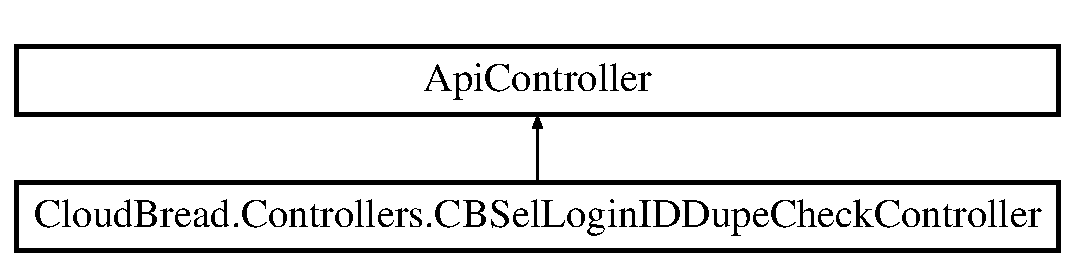
\includegraphics[height=2.000000cm]{a00050}
\end{center}
\end{figure}
\subsection*{Classes}
\begin{DoxyCompactItemize}
\item 
class \hyperlink{a00091}{Input\+Params}
\item 
class \hyperlink{a00174}{Result}
\end{DoxyCompactItemize}
\subsection*{Public Member Functions}
\begin{DoxyCompactItemize}
\item 
\hyperlink{a00174}{Result} {\bfseries Post} (\hyperlink{a00091}{Input\+Params} p)\hypertarget{a00050_ae6a1e88ad907f08f710be974100e1f17}{}\label{a00050_ae6a1e88ad907f08f710be974100e1f17}

\end{DoxyCompactItemize}


The documentation for this class was generated from the following file\+:\begin{DoxyCompactItemize}
\item 
C\+:/\+Users/dwkim/\+Documents/\+Git\+Hub/\+Cloud\+Bread/\+Cloud\+Bread/\+Controllers/\hyperlink{a00221}{C\+B\+Sel\+Login\+I\+D\+Dupe\+Check\+Controller.\+cs}\end{DoxyCompactItemize}

\hypertarget{a00051}{}\section{Cloud\+Bread.\+Models.\+Com\+Ins\+Member\+Item\+Purchase\+Input\+Params Class Reference}
\label{a00051}\index{Cloud\+Bread.\+Models.\+Com\+Ins\+Member\+Item\+Purchase\+Input\+Params@{Cloud\+Bread.\+Models.\+Com\+Ins\+Member\+Item\+Purchase\+Input\+Params}}
\subsection*{Properties}
\begin{DoxyCompactItemize}
\item 
string {\bfseries Member\+Item\+Purchase\+ID}\hspace{0.3cm}{\ttfamily  \mbox{[}get, set\mbox{]}}\hypertarget{a00051_aee2f4267120cf9719b80e82498948406}{}\label{a00051_aee2f4267120cf9719b80e82498948406}

\item 
string {\bfseries Member\+ID}\hspace{0.3cm}{\ttfamily  \mbox{[}get, set\mbox{]}}\hypertarget{a00051_a1250afa0d5b8808633b0265f620e4c99}{}\label{a00051_a1250afa0d5b8808633b0265f620e4c99}

\item 
string {\bfseries Item\+List\+ID}\hspace{0.3cm}{\ttfamily  \mbox{[}get, set\mbox{]}}\hypertarget{a00051_a5187a3316b757ae6af5665bed44abca8}{}\label{a00051_a5187a3316b757ae6af5665bed44abca8}

\item 
string {\bfseries Purchase\+Quantity}\hspace{0.3cm}{\ttfamily  \mbox{[}get, set\mbox{]}}\hypertarget{a00051_ae434af24080aaaae9f401598cf2c0bfe}{}\label{a00051_ae434af24080aaaae9f401598cf2c0bfe}

\item 
string {\bfseries Purchase\+Price}\hspace{0.3cm}{\ttfamily  \mbox{[}get, set\mbox{]}}\hypertarget{a00051_acc8edb60785c666a5e7a8d756834a1f4}{}\label{a00051_acc8edb60785c666a5e7a8d756834a1f4}

\item 
string {\bfseries P\+Ginfo1}\hspace{0.3cm}{\ttfamily  \mbox{[}get, set\mbox{]}}\hypertarget{a00051_a35b6475415ccdfabed1a10cea27f8735}{}\label{a00051_a35b6475415ccdfabed1a10cea27f8735}

\item 
string {\bfseries P\+Ginfo2}\hspace{0.3cm}{\ttfamily  \mbox{[}get, set\mbox{]}}\hypertarget{a00051_a6fd606f5d5aaf82429191f7fec25e7da}{}\label{a00051_a6fd606f5d5aaf82429191f7fec25e7da}

\item 
string {\bfseries P\+Ginfo3}\hspace{0.3cm}{\ttfamily  \mbox{[}get, set\mbox{]}}\hypertarget{a00051_a5acda290005e599d9438ecb2926c809a}{}\label{a00051_a5acda290005e599d9438ecb2926c809a}

\item 
string {\bfseries P\+Ginfo4}\hspace{0.3cm}{\ttfamily  \mbox{[}get, set\mbox{]}}\hypertarget{a00051_a9e3925f89ec00582f3a8a8b0024d06d4}{}\label{a00051_a9e3925f89ec00582f3a8a8b0024d06d4}

\item 
string {\bfseries P\+Ginfo5}\hspace{0.3cm}{\ttfamily  \mbox{[}get, set\mbox{]}}\hypertarget{a00051_ad5f7a30366d8986cffe85212c80b6e2a}{}\label{a00051_ad5f7a30366d8986cffe85212c80b6e2a}

\item 
string {\bfseries Purchase\+Device\+ID}\hspace{0.3cm}{\ttfamily  \mbox{[}get, set\mbox{]}}\hypertarget{a00051_a6f0543a1bea3da043cb467b36143ba8c}{}\label{a00051_a6f0543a1bea3da043cb467b36143ba8c}

\item 
string {\bfseries Purchase\+Device\+I\+P\+Address}\hspace{0.3cm}{\ttfamily  \mbox{[}get, set\mbox{]}}\hypertarget{a00051_a9a2916a7b8c030e7d977102874dd1494}{}\label{a00051_a9a2916a7b8c030e7d977102874dd1494}

\item 
string {\bfseries Purchase\+Device\+M\+A\+C\+Address}\hspace{0.3cm}{\ttfamily  \mbox{[}get, set\mbox{]}}\hypertarget{a00051_ae6ec4d4cf2545bb62720696b7008ed3b}{}\label{a00051_ae6ec4d4cf2545bb62720696b7008ed3b}

\item 
string {\bfseries Purchase\+DT}\hspace{0.3cm}{\ttfamily  \mbox{[}get, set\mbox{]}}\hypertarget{a00051_a0aadebdc20f55b03ec3fa6ae2b7db7e2}{}\label{a00051_a0aadebdc20f55b03ec3fa6ae2b7db7e2}

\item 
string {\bfseries Purchase\+Cancel\+YN}\hspace{0.3cm}{\ttfamily  \mbox{[}get, set\mbox{]}}\hypertarget{a00051_a8ca6bab4cc3e43125d845b30ac73606a}{}\label{a00051_a8ca6bab4cc3e43125d845b30ac73606a}

\item 
string {\bfseries Purchase\+Cancel\+DT}\hspace{0.3cm}{\ttfamily  \mbox{[}get, set\mbox{]}}\hypertarget{a00051_ab2f1e49658cbb5ba8c7fccf2014e4142}{}\label{a00051_ab2f1e49658cbb5ba8c7fccf2014e4142}

\item 
string {\bfseries Purchase\+Canceling\+Status}\hspace{0.3cm}{\ttfamily  \mbox{[}get, set\mbox{]}}\hypertarget{a00051_af9517672e93d34e98e4d1f7eb6572b24}{}\label{a00051_af9517672e93d34e98e4d1f7eb6572b24}

\item 
string {\bfseries Purchase\+Cancel\+Returned\+Amount}\hspace{0.3cm}{\ttfamily  \mbox{[}get, set\mbox{]}}\hypertarget{a00051_a6d18398a6c4e34d2e490fc7b936fa3e9}{}\label{a00051_a6d18398a6c4e34d2e490fc7b936fa3e9}

\item 
string {\bfseries Purchase\+Cancel\+Device\+ID}\hspace{0.3cm}{\ttfamily  \mbox{[}get, set\mbox{]}}\hypertarget{a00051_ab785c8befaab16e121f3f6ec1d5f1b7e}{}\label{a00051_ab785c8befaab16e121f3f6ec1d5f1b7e}

\item 
string {\bfseries Purchase\+Cancel\+Device\+I\+P\+Address}\hspace{0.3cm}{\ttfamily  \mbox{[}get, set\mbox{]}}\hypertarget{a00051_a298559fa171faaf67e8c28f7ad7ea443}{}\label{a00051_a298559fa171faaf67e8c28f7ad7ea443}

\item 
string {\bfseries Purchase\+Cancel\+Device\+M\+A\+C\+Address}\hspace{0.3cm}{\ttfamily  \mbox{[}get, set\mbox{]}}\hypertarget{a00051_a593161001620dbc1b72bbfe3a46a6614}{}\label{a00051_a593161001620dbc1b72bbfe3a46a6614}

\item 
string {\bfseries s\+Col1}\hspace{0.3cm}{\ttfamily  \mbox{[}get, set\mbox{]}}\hypertarget{a00051_a8cffb32d18cc24f21075c815d80a884d}{}\label{a00051_a8cffb32d18cc24f21075c815d80a884d}

\item 
string {\bfseries s\+Col2}\hspace{0.3cm}{\ttfamily  \mbox{[}get, set\mbox{]}}\hypertarget{a00051_a6e0f3a1b430141fc0b67db4f611ac3d0}{}\label{a00051_a6e0f3a1b430141fc0b67db4f611ac3d0}

\item 
string {\bfseries s\+Col3}\hspace{0.3cm}{\ttfamily  \mbox{[}get, set\mbox{]}}\hypertarget{a00051_ae8801be4130afe2248fafa1edaebb32d}{}\label{a00051_ae8801be4130afe2248fafa1edaebb32d}

\item 
string {\bfseries s\+Col4}\hspace{0.3cm}{\ttfamily  \mbox{[}get, set\mbox{]}}\hypertarget{a00051_ae09032c48fefe3c962d4f3716258eda8}{}\label{a00051_ae09032c48fefe3c962d4f3716258eda8}

\item 
string {\bfseries s\+Col5}\hspace{0.3cm}{\ttfamily  \mbox{[}get, set\mbox{]}}\hypertarget{a00051_a5b05b26e1f8ad68b813e1879f50a2f5b}{}\label{a00051_a5b05b26e1f8ad68b813e1879f50a2f5b}

\item 
string {\bfseries s\+Col6}\hspace{0.3cm}{\ttfamily  \mbox{[}get, set\mbox{]}}\hypertarget{a00051_a85f2ba6c9dd48ec203c2dd845dfe2ae7}{}\label{a00051_a85f2ba6c9dd48ec203c2dd845dfe2ae7}

\item 
string {\bfseries s\+Col7}\hspace{0.3cm}{\ttfamily  \mbox{[}get, set\mbox{]}}\hypertarget{a00051_ad4b2fc1b684e2b24dfe9d96230fc4669}{}\label{a00051_ad4b2fc1b684e2b24dfe9d96230fc4669}

\item 
string {\bfseries s\+Col8}\hspace{0.3cm}{\ttfamily  \mbox{[}get, set\mbox{]}}\hypertarget{a00051_a57d0082b701d1d009b068af5d5e6beb3}{}\label{a00051_a57d0082b701d1d009b068af5d5e6beb3}

\item 
string {\bfseries s\+Col9}\hspace{0.3cm}{\ttfamily  \mbox{[}get, set\mbox{]}}\hypertarget{a00051_aafefdc8c6bfe8cd73a686a64beb52866}{}\label{a00051_aafefdc8c6bfe8cd73a686a64beb52866}

\item 
string {\bfseries s\+Col10}\hspace{0.3cm}{\ttfamily  \mbox{[}get, set\mbox{]}}\hypertarget{a00051_a52bbee91e8589d1192e4b3c829696eee}{}\label{a00051_a52bbee91e8589d1192e4b3c829696eee}

\item 
string {\bfseries token}\hspace{0.3cm}{\ttfamily  \mbox{[}get, set\mbox{]}}\hypertarget{a00051_a6d378c66885ebfe59b85dcb836b6ce1f}{}\label{a00051_a6d378c66885ebfe59b85dcb836b6ce1f}

\end{DoxyCompactItemize}


The documentation for this class was generated from the following file\+:\begin{DoxyCompactItemize}
\item 
C\+:/\+Users/dwkim/\+Documents/\+Git\+Hub/\+Cloud\+Bread/\+Models/Com\+Ins\+Member\+Item\+Purchase.\+cs\end{DoxyCompactItemize}

\hypertarget{a00052}{}\section{Cloud\+Bread.\+Controllers.\+C\+B\+Sel\+Member\+Game\+Info\+Stages\+Controller Class Reference}
\label{a00052}\index{Cloud\+Bread.\+Controllers.\+C\+B\+Sel\+Member\+Game\+Info\+Stages\+Controller@{Cloud\+Bread.\+Controllers.\+C\+B\+Sel\+Member\+Game\+Info\+Stages\+Controller}}
Inheritance diagram for Cloud\+Bread.\+Controllers.\+C\+B\+Sel\+Member\+Game\+Info\+Stages\+Controller\+:\begin{figure}[H]
\begin{center}
\leavevmode
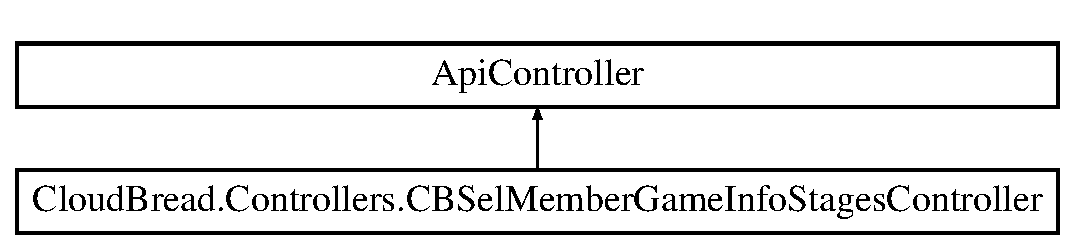
\includegraphics[height=2.000000cm]{a00052}
\end{center}
\end{figure}
\subsection*{Classes}
\begin{DoxyCompactItemize}
\item 
class \hyperlink{a00096}{Input\+Params}
\item 
class \hyperlink{a00154}{Model}
\end{DoxyCompactItemize}
\subsection*{Public Member Functions}
\begin{DoxyCompactItemize}
\item 
List$<$ \hyperlink{a00154}{Model} $>$ {\bfseries Post} (\hyperlink{a00096}{Input\+Params} p)\hypertarget{a00052_a115131232527678f913beb72c337143e}{}\label{a00052_a115131232527678f913beb72c337143e}

\end{DoxyCompactItemize}


The documentation for this class was generated from the following file\+:\begin{DoxyCompactItemize}
\item 
C\+:/\+Users/dwkim/\+Documents/\+Git\+Hub/\+Cloud\+Bread/\+Cloud\+Bread/\+Controllers/\hyperlink{a00223}{C\+B\+Sel\+Member\+Game\+Info\+Stages\+Controller.\+cs}\end{DoxyCompactItemize}

\hypertarget{a00053}{}\section{Cloud\+Bread.\+Controllers.\+C\+B\+Sel\+Member\+Items\+Controller Class Reference}
\label{a00053}\index{Cloud\+Bread.\+Controllers.\+C\+B\+Sel\+Member\+Items\+Controller@{Cloud\+Bread.\+Controllers.\+C\+B\+Sel\+Member\+Items\+Controller}}
Inheritance diagram for Cloud\+Bread.\+Controllers.\+C\+B\+Sel\+Member\+Items\+Controller\+:\begin{figure}[H]
\begin{center}
\leavevmode
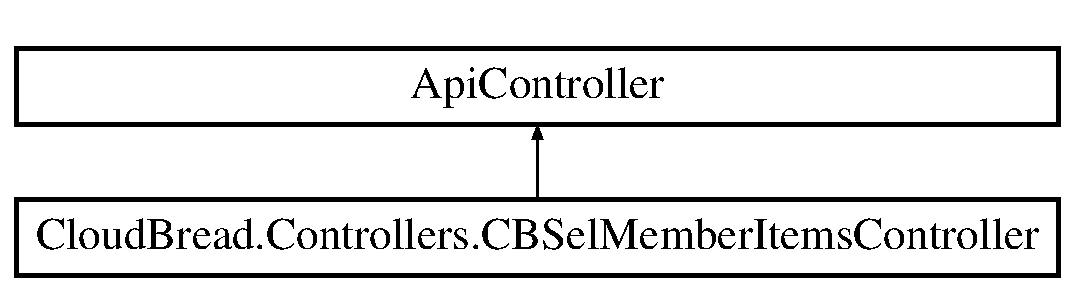
\includegraphics[height=2.000000cm]{a00053}
\end{center}
\end{figure}
\subsection*{Classes}
\begin{DoxyCompactItemize}
\item 
class \hyperlink{a00098}{Input\+Params}
\item 
class \hyperlink{a00163}{Model}
\end{DoxyCompactItemize}
\subsection*{Public Member Functions}
\begin{DoxyCompactItemize}
\item 
List$<$ \hyperlink{a00163}{Model} $>$ {\bfseries Post} (\hyperlink{a00098}{Input\+Params} p)\hypertarget{a00053_a5e7fe0d95c6b9364f552f15e007f5acd}{}\label{a00053_a5e7fe0d95c6b9364f552f15e007f5acd}

\end{DoxyCompactItemize}


The documentation for this class was generated from the following file\+:\begin{DoxyCompactItemize}
\item 
C\+:/\+Users/dwkim/\+Documents/\+Git\+Hub/\+Cloud\+Bread/\+Cloud\+Bread/\+Controllers/\hyperlink{a00224}{C\+B\+Sel\+Member\+Items\+Controller.\+cs}\end{DoxyCompactItemize}

\hypertarget{a00054}{}\section{Cloud\+Bread.\+Models.\+Com\+Sel\+Gift\+Depository\+Input\+Params Class Reference}
\label{a00054}\index{Cloud\+Bread.\+Models.\+Com\+Sel\+Gift\+Depository\+Input\+Params@{Cloud\+Bread.\+Models.\+Com\+Sel\+Gift\+Depository\+Input\+Params}}
\subsection*{Public Attributes}
\begin{DoxyCompactItemize}
\item 
string {\bfseries Member\+ID}\hypertarget{a00054_acbe64b4f10384a97b625930589a03b95}{}\label{a00054_acbe64b4f10384a97b625930589a03b95}

\item 
string {\bfseries Gift\+Depository\+ID}\hypertarget{a00054_a2102851db1dc7a7a8080ad36fc16eef3}{}\label{a00054_a2102851db1dc7a7a8080ad36fc16eef3}

\item 
string {\bfseries token}\hypertarget{a00054_ad6aba426bef607419382284c00d2d3dc}{}\label{a00054_ad6aba426bef607419382284c00d2d3dc}

\end{DoxyCompactItemize}


The documentation for this class was generated from the following file\+:\begin{DoxyCompactItemize}
\item 
C\+:/\+Users/dwkim/\+Documents/\+Git\+Hub/\+Cloud\+Bread/\+Models/Com\+Sel\+Gift\+Depository.\+cs\end{DoxyCompactItemize}

\hypertarget{a00055}{}\section{Cloud\+Bread.\+Controllers.\+C\+B\+Sel\+Send\+Email\+To\+Member\+Controller Class Reference}
\label{a00055}\index{Cloud\+Bread.\+Controllers.\+C\+B\+Sel\+Send\+Email\+To\+Member\+Controller@{Cloud\+Bread.\+Controllers.\+C\+B\+Sel\+Send\+Email\+To\+Member\+Controller}}
Inheritance diagram for Cloud\+Bread.\+Controllers.\+C\+B\+Sel\+Send\+Email\+To\+Member\+Controller\+:\begin{figure}[H]
\begin{center}
\leavevmode
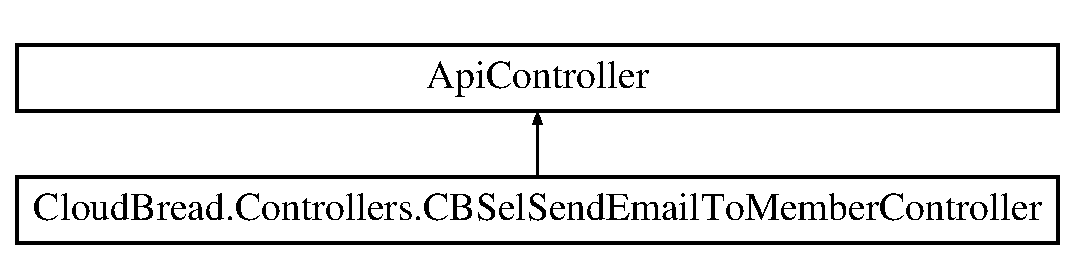
\includegraphics[height=2.000000cm]{a00055}
\end{center}
\end{figure}
\subsection*{Classes}
\begin{DoxyCompactItemize}
\item 
class \hyperlink{a00104}{Input\+Params}
\end{DoxyCompactItemize}
\subsection*{Public Member Functions}
\begin{DoxyCompactItemize}
\item 
string {\bfseries Post} (\hyperlink{a00104}{Input\+Params} p)\hypertarget{a00055_a1e0e460211039ff78137d64d7d4a1958}{}\label{a00055_a1e0e460211039ff78137d64d7d4a1958}

\end{DoxyCompactItemize}


The documentation for this class was generated from the following file\+:\begin{DoxyCompactItemize}
\item 
C\+:/\+Users/dwkim/\+Documents/\+Git\+Hub/\+Cloud\+Bread/\+Cloud\+Bread/\+Controllers/\hyperlink{a00226}{C\+B\+Sel\+Send\+Email\+To\+Member\+Controller.\+cs}\end{DoxyCompactItemize}

\hypertarget{a00056}{}\section{Cloud\+Bread.\+Models.\+Com\+Sel\+Item\+List1\+Input\+Params Class Reference}
\label{a00056}\index{Cloud\+Bread.\+Models.\+Com\+Sel\+Item\+List1\+Input\+Params@{Cloud\+Bread.\+Models.\+Com\+Sel\+Item\+List1\+Input\+Params}}
\subsection*{Public Attributes}
\begin{DoxyCompactItemize}
\item 
string {\bfseries Member\+ID}\hypertarget{a00056_a56ea09ae3fed36e05cb415874169d7b3}{}\label{a00056_a56ea09ae3fed36e05cb415874169d7b3}

\item 
string {\bfseries Item\+List\+ID}\hypertarget{a00056_aa06d87b5fbd1a9fab11288cb0d55d36a}{}\label{a00056_aa06d87b5fbd1a9fab11288cb0d55d36a}

\item 
string {\bfseries token}\hypertarget{a00056_a9e7daa23318bd51e9ed2d7e992d26c4d}{}\label{a00056_a9e7daa23318bd51e9ed2d7e992d26c4d}

\end{DoxyCompactItemize}


The documentation for this class was generated from the following file\+:\begin{DoxyCompactItemize}
\item 
C\+:/\+Users/dwkim/\+Documents/\+Git\+Hub/\+Cloud\+Bread/\+Models/Com\+Sel\+Item\+List1.\+cs\end{DoxyCompactItemize}

\hypertarget{a00057}{}\section{Cloud\+Bread.\+Controllers.\+C\+B\+Udt\+Coupon\+Member\+Controller Class Reference}
\label{a00057}\index{Cloud\+Bread.\+Controllers.\+C\+B\+Udt\+Coupon\+Member\+Controller@{Cloud\+Bread.\+Controllers.\+C\+B\+Udt\+Coupon\+Member\+Controller}}
Inheritance diagram for Cloud\+Bread.\+Controllers.\+C\+B\+Udt\+Coupon\+Member\+Controller\+:\begin{figure}[H]
\begin{center}
\leavevmode
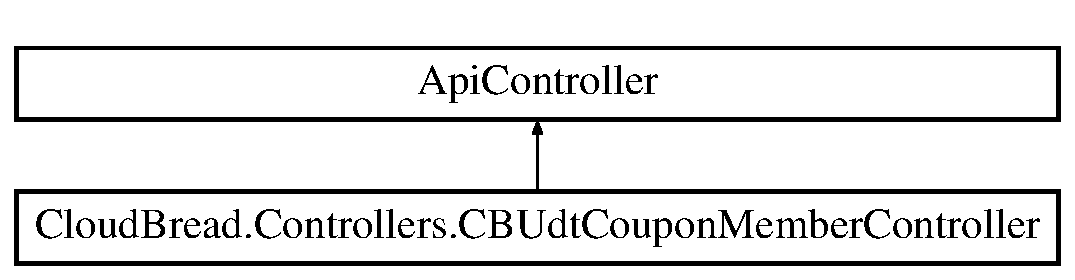
\includegraphics[height=2.000000cm]{a00057}
\end{center}
\end{figure}
\subsection*{Classes}
\begin{DoxyCompactItemize}
\item 
class \hyperlink{a00107}{Input\+Params}
\end{DoxyCompactItemize}
\subsection*{Public Member Functions}
\begin{DoxyCompactItemize}
\item 
string {\bfseries Post} (\hyperlink{a00107}{Input\+Params} p)\hypertarget{a00057_a55a2e1a6013d3916235ccd6054efb91e}{}\label{a00057_a55a2e1a6013d3916235ccd6054efb91e}

\end{DoxyCompactItemize}


The documentation for this class was generated from the following file\+:\begin{DoxyCompactItemize}
\item 
C\+:/\+Users/dwkim/\+Documents/\+Git\+Hub/\+Cloud\+Bread/\+Cloud\+Bread/\+Controllers/\hyperlink{a00228}{C\+B\+Udt\+Coupon\+Member\+Controller.\+cs}\end{DoxyCompactItemize}

\hypertarget{a00058}{}\section{Cloud\+Bread.\+Models.\+Com\+Sel\+Member\+Game\+Infoes\+Input\+Params Class Reference}
\label{a00058}\index{Cloud\+Bread.\+Models.\+Com\+Sel\+Member\+Game\+Infoes\+Input\+Params@{Cloud\+Bread.\+Models.\+Com\+Sel\+Member\+Game\+Infoes\+Input\+Params}}
\subsection*{Properties}
\begin{DoxyCompactItemize}
\item 
string {\bfseries Member\+ID}\hspace{0.3cm}{\ttfamily  \mbox{[}get, set\mbox{]}}\hypertarget{a00058_a9d4bf4f11c41460246c2d359ef8101e5}{}\label{a00058_a9d4bf4f11c41460246c2d359ef8101e5}

\item 
string {\bfseries token}\hspace{0.3cm}{\ttfamily  \mbox{[}get, set\mbox{]}}\hypertarget{a00058_acf1b5e6f724f126b892a6415c5fb8059}{}\label{a00058_acf1b5e6f724f126b892a6415c5fb8059}

\end{DoxyCompactItemize}


The documentation for this class was generated from the following file\+:\begin{DoxyCompactItemize}
\item 
C\+:/\+Users/dwkim/\+Documents/\+Git\+Hub/\+Cloud\+Bread/\+Models/Com\+Sel\+Member\+Game\+Infoes.\+cs\end{DoxyCompactItemize}

\hypertarget{a00059}{}\section{Cloud\+Bread.\+Models.\+Com\+Sel\+Member\+Game\+Infoes\+Model Class Reference}
\label{a00059}\index{Cloud\+Bread.\+Models.\+Com\+Sel\+Member\+Game\+Infoes\+Model@{Cloud\+Bread.\+Models.\+Com\+Sel\+Member\+Game\+Infoes\+Model}}
\subsection*{Properties}
\begin{DoxyCompactItemize}
\item 
string {\bfseries Member\+ID}\hspace{0.3cm}{\ttfamily  \mbox{[}get, set\mbox{]}}\hypertarget{a00059_af2f18424328ad140e55742ad10ce71bb}{}\label{a00059_af2f18424328ad140e55742ad10ce71bb}

\item 
string {\bfseries Level}\hspace{0.3cm}{\ttfamily  \mbox{[}get, set\mbox{]}}\hypertarget{a00059_ac18ac07bb77e290e7fd16d42e8357f37}{}\label{a00059_ac18ac07bb77e290e7fd16d42e8357f37}

\item 
string {\bfseries Exps}\hspace{0.3cm}{\ttfamily  \mbox{[}get, set\mbox{]}}\hypertarget{a00059_ae8dda543f0ecd7abb48b729221e1c6f6}{}\label{a00059_ae8dda543f0ecd7abb48b729221e1c6f6}

\item 
string {\bfseries Points}\hspace{0.3cm}{\ttfamily  \mbox{[}get, set\mbox{]}}\hypertarget{a00059_a68b7fa957f9a1e19b21f1e09fb5ea5a2}{}\label{a00059_a68b7fa957f9a1e19b21f1e09fb5ea5a2}

\item 
string {\bfseries User\+S\+T\+A\+T1}\hspace{0.3cm}{\ttfamily  \mbox{[}get, set\mbox{]}}\hypertarget{a00059_af71c1fbb8ab4b55d7bf6c8e6c992e7a3}{}\label{a00059_af71c1fbb8ab4b55d7bf6c8e6c992e7a3}

\item 
string {\bfseries User\+S\+T\+A\+T2}\hspace{0.3cm}{\ttfamily  \mbox{[}get, set\mbox{]}}\hypertarget{a00059_a1c33690ec65b9ea88bd3c8a1992f559d}{}\label{a00059_a1c33690ec65b9ea88bd3c8a1992f559d}

\item 
string {\bfseries User\+S\+T\+A\+T3}\hspace{0.3cm}{\ttfamily  \mbox{[}get, set\mbox{]}}\hypertarget{a00059_af35420e9608fc20c856fe56f16940a5e}{}\label{a00059_af35420e9608fc20c856fe56f16940a5e}

\item 
string {\bfseries User\+S\+T\+A\+T4}\hspace{0.3cm}{\ttfamily  \mbox{[}get, set\mbox{]}}\hypertarget{a00059_a86e9c0ef865fab86fefce5a64c5b6a3d}{}\label{a00059_a86e9c0ef865fab86fefce5a64c5b6a3d}

\item 
string {\bfseries User\+S\+T\+A\+T5}\hspace{0.3cm}{\ttfamily  \mbox{[}get, set\mbox{]}}\hypertarget{a00059_a883ef3c2ed0dbd9bf113e255f5f5eb56}{}\label{a00059_a883ef3c2ed0dbd9bf113e255f5f5eb56}

\item 
string {\bfseries User\+S\+T\+A\+T6}\hspace{0.3cm}{\ttfamily  \mbox{[}get, set\mbox{]}}\hypertarget{a00059_af677d07aa570502bd5688dbdda8dec09}{}\label{a00059_af677d07aa570502bd5688dbdda8dec09}

\item 
string {\bfseries User\+S\+T\+A\+T7}\hspace{0.3cm}{\ttfamily  \mbox{[}get, set\mbox{]}}\hypertarget{a00059_a89853dfb249bcab6f9a9fe446fa2aba7}{}\label{a00059_a89853dfb249bcab6f9a9fe446fa2aba7}

\item 
string {\bfseries User\+S\+T\+A\+T8}\hspace{0.3cm}{\ttfamily  \mbox{[}get, set\mbox{]}}\hypertarget{a00059_a1470bde9650a7ee049b4152f2fcf0cb6}{}\label{a00059_a1470bde9650a7ee049b4152f2fcf0cb6}

\item 
string {\bfseries User\+S\+T\+A\+T9}\hspace{0.3cm}{\ttfamily  \mbox{[}get, set\mbox{]}}\hypertarget{a00059_af169dd6207b0cf9965961da94f3a701e}{}\label{a00059_af169dd6207b0cf9965961da94f3a701e}

\item 
string {\bfseries User\+S\+T\+A\+T10}\hspace{0.3cm}{\ttfamily  \mbox{[}get, set\mbox{]}}\hypertarget{a00059_ad226d4e297125a23c972a63427f7effc}{}\label{a00059_ad226d4e297125a23c972a63427f7effc}

\item 
string {\bfseries s\+Col1}\hspace{0.3cm}{\ttfamily  \mbox{[}get, set\mbox{]}}\hypertarget{a00059_a1cf69a0c8e425e7253cba64942dff708}{}\label{a00059_a1cf69a0c8e425e7253cba64942dff708}

\item 
string {\bfseries s\+Col2}\hspace{0.3cm}{\ttfamily  \mbox{[}get, set\mbox{]}}\hypertarget{a00059_ab794cf359d1cea5d5bd4d4e9876f319e}{}\label{a00059_ab794cf359d1cea5d5bd4d4e9876f319e}

\item 
string {\bfseries s\+Col3}\hspace{0.3cm}{\ttfamily  \mbox{[}get, set\mbox{]}}\hypertarget{a00059_a4ff4808f1c611f98633869e29a3dc2e1}{}\label{a00059_a4ff4808f1c611f98633869e29a3dc2e1}

\item 
string {\bfseries s\+Col4}\hspace{0.3cm}{\ttfamily  \mbox{[}get, set\mbox{]}}\hypertarget{a00059_a5345ad0e943de50af8e7799f83a3afab}{}\label{a00059_a5345ad0e943de50af8e7799f83a3afab}

\item 
string {\bfseries s\+Col5}\hspace{0.3cm}{\ttfamily  \mbox{[}get, set\mbox{]}}\hypertarget{a00059_a3685ae6866dd991cd43bcfe3ea44a0f6}{}\label{a00059_a3685ae6866dd991cd43bcfe3ea44a0f6}

\item 
string {\bfseries s\+Col6}\hspace{0.3cm}{\ttfamily  \mbox{[}get, set\mbox{]}}\hypertarget{a00059_abb865f2f09e52fe29342f7c68d412e1e}{}\label{a00059_abb865f2f09e52fe29342f7c68d412e1e}

\item 
string {\bfseries s\+Col7}\hspace{0.3cm}{\ttfamily  \mbox{[}get, set\mbox{]}}\hypertarget{a00059_a5b3c51e2c01591c3bb246fbb889ee2c3}{}\label{a00059_a5b3c51e2c01591c3bb246fbb889ee2c3}

\item 
string {\bfseries s\+Col8}\hspace{0.3cm}{\ttfamily  \mbox{[}get, set\mbox{]}}\hypertarget{a00059_a7ca71320035d93755f573457c83fc1f1}{}\label{a00059_a7ca71320035d93755f573457c83fc1f1}

\item 
string {\bfseries s\+Col9}\hspace{0.3cm}{\ttfamily  \mbox{[}get, set\mbox{]}}\hypertarget{a00059_a44e121402c7ed38a6498a6c5316c41f8}{}\label{a00059_a44e121402c7ed38a6498a6c5316c41f8}

\item 
string {\bfseries s\+Col10}\hspace{0.3cm}{\ttfamily  \mbox{[}get, set\mbox{]}}\hypertarget{a00059_ae816caa1d7922f2a608f463f89f4be1b}{}\label{a00059_ae816caa1d7922f2a608f463f89f4be1b}

\end{DoxyCompactItemize}


The documentation for this class was generated from the following file\+:\begin{DoxyCompactItemize}
\item 
C\+:/\+Users/dwkim/\+Documents/\+Git\+Hub/\+Cloud\+Bread/\+Models/Com\+Sel\+Member\+Game\+Infoes.\+cs\end{DoxyCompactItemize}

\hypertarget{a00060}{}\section{Cloud\+Bread.\+Models.\+Com\+Sel\+Member\+Game\+Info\+Stages\+Input\+Params Class Reference}
\label{a00060}\index{Cloud\+Bread.\+Models.\+Com\+Sel\+Member\+Game\+Info\+Stages\+Input\+Params@{Cloud\+Bread.\+Models.\+Com\+Sel\+Member\+Game\+Info\+Stages\+Input\+Params}}
\subsection*{Properties}
\begin{DoxyCompactItemize}
\item 
string {\bfseries Member\+ID}\hspace{0.3cm}{\ttfamily  \mbox{[}get, set\mbox{]}}\hypertarget{a00060_a50431f69daed8c937ad8c3f7cdf29055}{}\label{a00060_a50431f69daed8c937ad8c3f7cdf29055}

\item 
string {\bfseries Member\+Game\+Info\+Stage\+ID}\hspace{0.3cm}{\ttfamily  \mbox{[}get, set\mbox{]}}\hypertarget{a00060_a2f3d1384c88c08d21cd982ade426b89d}{}\label{a00060_a2f3d1384c88c08d21cd982ade426b89d}

\item 
string {\bfseries token}\hspace{0.3cm}{\ttfamily  \mbox{[}get, set\mbox{]}}\hypertarget{a00060_a308bf9d8d4c06162e070c1488785b110}{}\label{a00060_a308bf9d8d4c06162e070c1488785b110}

\end{DoxyCompactItemize}


The documentation for this class was generated from the following file\+:\begin{DoxyCompactItemize}
\item 
C\+:/\+Users/dwkim/\+Documents/\+Git\+Hub/\+Cloud\+Bread/\+Models/Com\+Sel\+Member\+Game\+Info\+Stages.\+cs\end{DoxyCompactItemize}

\hypertarget{a00061}{}\section{Cloud\+Bread.\+Controllers.\+C\+B\+Udt\+Return\+Item\+Controller Class Reference}
\label{a00061}\index{Cloud\+Bread.\+Controllers.\+C\+B\+Udt\+Return\+Item\+Controller@{Cloud\+Bread.\+Controllers.\+C\+B\+Udt\+Return\+Item\+Controller}}
Inheritance diagram for Cloud\+Bread.\+Controllers.\+C\+B\+Udt\+Return\+Item\+Controller\+:\begin{figure}[H]
\begin{center}
\leavevmode
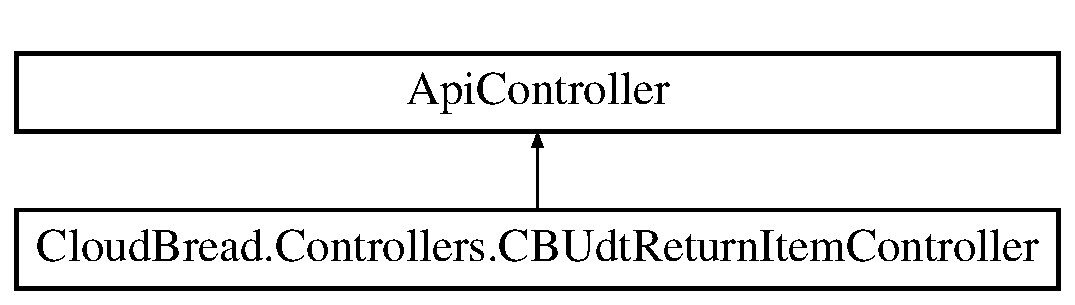
\includegraphics[height=2.000000cm]{a00061}
\end{center}
\end{figure}
\subsection*{Classes}
\begin{DoxyCompactItemize}
\item 
class \hyperlink{a00118}{Input\+Params}
\end{DoxyCompactItemize}
\subsection*{Public Member Functions}
\begin{DoxyCompactItemize}
\item 
string {\bfseries Post} (\hyperlink{a00118}{Input\+Params} p)\hypertarget{a00061_a87a08b50ec73fd4f516a143dbd8e9ec0}{}\label{a00061_a87a08b50ec73fd4f516a143dbd8e9ec0}

\end{DoxyCompactItemize}


The documentation for this class was generated from the following file\+:\begin{DoxyCompactItemize}
\item 
C\+:/\+Users/dwkim/\+Documents/\+Git\+Hub/\+Cloud\+Bread/\+Cloud\+Bread/\+Controllers/\hyperlink{a00234}{C\+D\+Udt\+Return\+Item\+Controller.\+cs}\end{DoxyCompactItemize}

\hypertarget{a00062}{}\section{Cloud\+Bread.\+Controllers.\+C\+B\+Udt\+Sell\+Item\+Controller Class Reference}
\label{a00062}\index{Cloud\+Bread.\+Controllers.\+C\+B\+Udt\+Sell\+Item\+Controller@{Cloud\+Bread.\+Controllers.\+C\+B\+Udt\+Sell\+Item\+Controller}}
Inheritance diagram for Cloud\+Bread.\+Controllers.\+C\+B\+Udt\+Sell\+Item\+Controller\+:\begin{figure}[H]
\begin{center}
\leavevmode
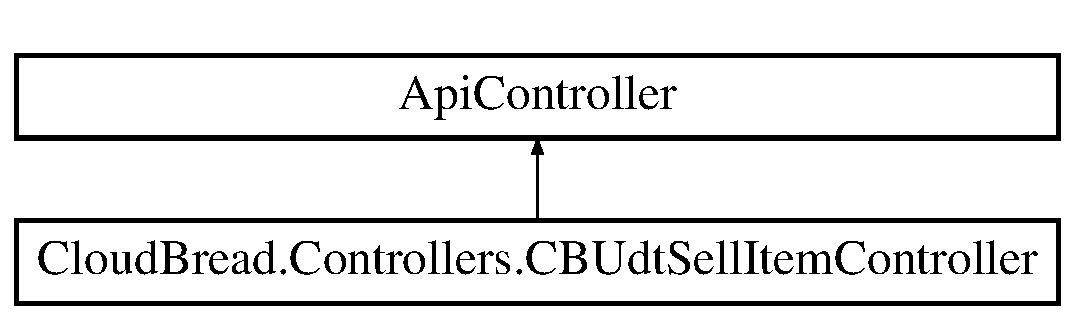
\includegraphics[height=2.000000cm]{a00062}
\end{center}
\end{figure}


The documentation for this class was generated from the following file\+:\begin{DoxyCompactItemize}
\item 
C\+:/\+Users/dwkim/\+Documents/\+Git\+Hub/\+Cloud\+Bread/\+Cloud\+Bread/\+Controllers/\hyperlink{a00232}{C\+B\+Udt\+Sell\+Item\+Controller.\+cs}\end{DoxyCompactItemize}

\hypertarget{a00063}{}\section{Cloud\+Bread.\+Controllers.\+C\+B\+Udt\+Send\+Gift\+Controller Class Reference}
\label{a00063}\index{Cloud\+Bread.\+Controllers.\+C\+B\+Udt\+Send\+Gift\+Controller@{Cloud\+Bread.\+Controllers.\+C\+B\+Udt\+Send\+Gift\+Controller}}
Inheritance diagram for Cloud\+Bread.\+Controllers.\+C\+B\+Udt\+Send\+Gift\+Controller\+:\begin{figure}[H]
\begin{center}
\leavevmode
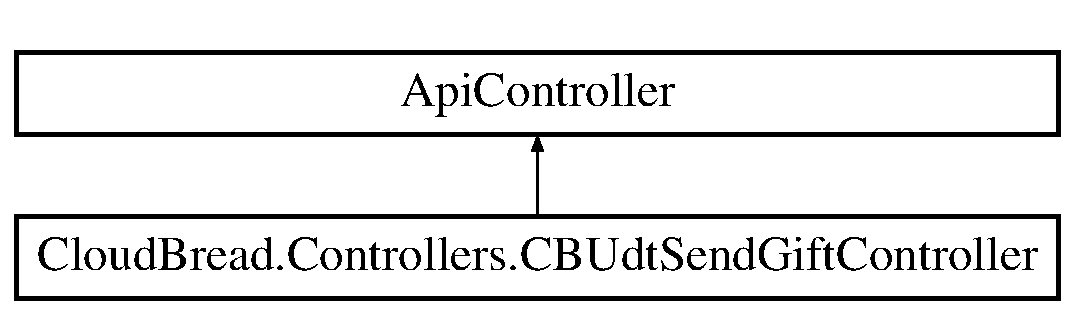
\includegraphics[height=2.000000cm]{a00063}
\end{center}
\end{figure}
\subsection*{Classes}
\begin{DoxyCompactItemize}
\item 
class \hyperlink{a00116}{Input\+Params}
\end{DoxyCompactItemize}
\subsection*{Public Member Functions}
\begin{DoxyCompactItemize}
\item 
string {\bfseries Post} (\hyperlink{a00116}{Input\+Params} p)\hypertarget{a00063_a4076720fd05860f0eec62024465afdb3}{}\label{a00063_a4076720fd05860f0eec62024465afdb3}

\end{DoxyCompactItemize}


The documentation for this class was generated from the following file\+:\begin{DoxyCompactItemize}
\item 
C\+:/\+Users/dwkim/\+Documents/\+Git\+Hub/\+Cloud\+Bread/\+Cloud\+Bread/\+Controllers/\hyperlink{a00233}{C\+B\+Udt\+Send\+Gift\+Controller.\+cs}\end{DoxyCompactItemize}

\hypertarget{a00064}{}\section{Cloud\+Bread\+Admin\+Web.\+Models.\+Change\+Password\+View\+Model Class Reference}
\label{a00064}\index{Cloud\+Bread\+Admin\+Web.\+Models.\+Change\+Password\+View\+Model@{Cloud\+Bread\+Admin\+Web.\+Models.\+Change\+Password\+View\+Model}}
\subsection*{Properties}
\begin{DoxyCompactItemize}
\item 
string {\bfseries Old\+Password}\hspace{0.3cm}{\ttfamily  \mbox{[}get, set\mbox{]}}\hypertarget{a00064_ad13c5856dd47f45c11abf687622dd72b}{}\label{a00064_ad13c5856dd47f45c11abf687622dd72b}

\item 
string {\bfseries New\+Password}\hspace{0.3cm}{\ttfamily  \mbox{[}get, set\mbox{]}}\hypertarget{a00064_a57f7addf7cf3000d14eba846774ae494}{}\label{a00064_a57f7addf7cf3000d14eba846774ae494}

\item 
string {\bfseries Confirm\+Password}\hspace{0.3cm}{\ttfamily  \mbox{[}get, set\mbox{]}}\hypertarget{a00064_ab3ce99d097dc66a28bb1757726a9e7f3}{}\label{a00064_ab3ce99d097dc66a28bb1757726a9e7f3}

\end{DoxyCompactItemize}


The documentation for this class was generated from the following file\+:\begin{DoxyCompactItemize}
\item 
C\+:/\+Users/dwkim/\+Documents/\+Git\+Hub/\+Cloud\+Bread/\+Cloud\+Bread\+Admin\+Web/\+Models/Manage\+View\+Models.\+cs\end{DoxyCompactItemize}

\hypertarget{a00065}{}\section{Cloud\+Bread\+Admin\+Web.\+Cloud\+Bread\+D\+B\+Admin\+Entities Class Reference}
\label{a00065}\index{Cloud\+Bread\+Admin\+Web.\+Cloud\+Bread\+D\+B\+Admin\+Entities@{Cloud\+Bread\+Admin\+Web.\+Cloud\+Bread\+D\+B\+Admin\+Entities}}
Inheritance diagram for Cloud\+Bread\+Admin\+Web.\+Cloud\+Bread\+D\+B\+Admin\+Entities\+:\begin{figure}[H]
\begin{center}
\leavevmode
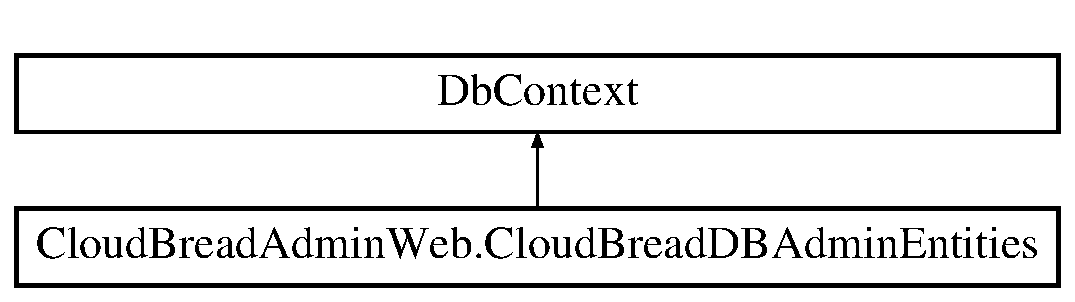
\includegraphics[height=2.000000cm]{a00065}
\end{center}
\end{figure}
\subsection*{Protected Member Functions}
\begin{DoxyCompactItemize}
\item 
override void {\bfseries On\+Model\+Creating} (Db\+Model\+Builder model\+Builder)\hypertarget{a00065_a5ccd5188cb9e1f2e6d2b679507002edb}{}\label{a00065_a5ccd5188cb9e1f2e6d2b679507002edb}

\end{DoxyCompactItemize}
\subsection*{Properties}
\begin{DoxyCompactItemize}
\item 
virtual Db\+Set$<$ \hyperlink{a00012}{Admin\+Members} $>$ {\bfseries Admin\+Members}\hspace{0.3cm}{\ttfamily  \mbox{[}get, set\mbox{]}}\hypertarget{a00065_adbbfd5b92d30b2fb24d618435ce9a9b9}{}\label{a00065_adbbfd5b92d30b2fb24d618435ce9a9b9}

\item 
virtual Db\+Set$<$ \hyperlink{a00127}{Item\+Lists} $>$ {\bfseries Item\+Lists}\hspace{0.3cm}{\ttfamily  \mbox{[}get, set\mbox{]}}\hypertarget{a00065_aee0437c77e1b4c5961f5811281234b66}{}\label{a00065_aee0437c77e1b4c5961f5811281234b66}

\item 
virtual Db\+Set$<$ \hyperlink{a00185}{Stats\+Data} $>$ {\bfseries Stats\+Data}\hspace{0.3cm}{\ttfamily  \mbox{[}get, set\mbox{]}}\hypertarget{a00065_a03c5e7ad00f935aecbd55470b199b225}{}\label{a00065_a03c5e7ad00f935aecbd55470b199b225}

\item 
virtual Db\+Set$<$ \hyperlink{a00143}{Member\+Items} $>$ {\bfseries Member\+Items}\hspace{0.3cm}{\ttfamily  \mbox{[}get, set\mbox{]}}\hypertarget{a00065_a26806075e48f05eca9fdcb38c9c6e6aa}{}\label{a00065_a26806075e48f05eca9fdcb38c9c6e6aa}

\item 
virtual Db\+Set$<$ \hyperlink{a00068}{Coupon} $>$ {\bfseries Coupon}\hspace{0.3cm}{\ttfamily  \mbox{[}get, set\mbox{]}}\hypertarget{a00065_a4229fde1faf3b715b44f3e9925b2efc2}{}\label{a00065_a4229fde1faf3b715b44f3e9925b2efc2}

\item 
virtual Db\+Set$<$ \hyperlink{a00069}{Coupon\+Member} $>$ {\bfseries Coupon\+Member}\hspace{0.3cm}{\ttfamily  \mbox{[}get, set\mbox{]}}\hypertarget{a00065_aeddd37d96d7580196dfdcb5ebe3bbf2e}{}\label{a00065_aeddd37d96d7580196dfdcb5ebe3bbf2e}

\item 
virtual Db\+Set$<$ \hyperlink{a00081}{Game\+Event\+Member} $>$ {\bfseries Game\+Event\+Member}\hspace{0.3cm}{\ttfamily  \mbox{[}get, set\mbox{]}}\hypertarget{a00065_afc122a11fdc5c4f293e730742d29a64c}{}\label{a00065_afc122a11fdc5c4f293e730742d29a64c}

\item 
virtual Db\+Set$<$ \hyperlink{a00083}{Game\+Events} $>$ {\bfseries Game\+Events}\hspace{0.3cm}{\ttfamily  \mbox{[}get, set\mbox{]}}\hypertarget{a00065_a16fffa8f4637449b5e3f2db3afee1e06}{}\label{a00065_a16fffa8f4637449b5e3f2db3afee1e06}

\item 
virtual Db\+Set$<$ \hyperlink{a00086}{Gift\+Depositories} $>$ {\bfseries Gift\+Depositories}\hspace{0.3cm}{\ttfamily  \mbox{[}get, set\mbox{]}}\hypertarget{a00065_aab20cb8f0bdfb846057cbcb1f18969f6}{}\label{a00065_aab20cb8f0bdfb846057cbcb1f18969f6}

\item 
virtual Db\+Set$<$ \hyperlink{a00135}{Member\+Account\+Block\+Log} $>$ {\bfseries Member\+Account\+Block\+Log}\hspace{0.3cm}{\ttfamily  \mbox{[}get, set\mbox{]}}\hypertarget{a00065_ac4fe771e2a7b3c8b38b6f8995d996425}{}\label{a00065_ac4fe771e2a7b3c8b38b6f8995d996425}

\item 
virtual Db\+Set$<$ \hyperlink{a00137}{Member\+Game\+Infoes} $>$ {\bfseries Member\+Game\+Infoes}\hspace{0.3cm}{\ttfamily  \mbox{[}get, set\mbox{]}}\hypertarget{a00065_a9d100a658fca7ffe660f1d8cc2f9b1fe}{}\label{a00065_a9d100a658fca7ffe660f1d8cc2f9b1fe}

\item 
virtual Db\+Set$<$ \hyperlink{a00139}{Member\+Game\+Info\+Stages} $>$ {\bfseries Member\+Game\+Info\+Stages}\hspace{0.3cm}{\ttfamily  \mbox{[}get, set\mbox{]}}\hypertarget{a00065_a068e8c53f6de34b24adbe7b5fc7b8ee9}{}\label{a00065_a068e8c53f6de34b24adbe7b5fc7b8ee9}

\item 
virtual Db\+Set$<$ \hyperlink{a00141}{Member\+Item\+Purchases} $>$ {\bfseries Member\+Item\+Purchases}\hspace{0.3cm}{\ttfamily  \mbox{[}get, set\mbox{]}}\hypertarget{a00065_aa7ca3897a4f4a4a687e0dc60ebfe2476}{}\label{a00065_aa7ca3897a4f4a4a687e0dc60ebfe2476}

\item 
virtual Db\+Set$<$ \hyperlink{a00145}{Members} $>$ {\bfseries Members}\hspace{0.3cm}{\ttfamily  \mbox{[}get, set\mbox{]}}\hypertarget{a00065_a38c8f483ece9bae4844f446d481e8766}{}\label{a00065_a38c8f483ece9bae4844f446d481e8766}

\item 
virtual Db\+Set$<$ \hyperlink{a00168}{Notices} $>$ {\bfseries Notices}\hspace{0.3cm}{\ttfamily  \mbox{[}get, set\mbox{]}}\hypertarget{a00065_acba614f544c7cac3062e5cf23e3f7ba1}{}\label{a00065_acba614f544c7cac3062e5cf23e3f7ba1}

\item 
virtual Db\+Set$<$ \hyperlink{a00178}{Server\+Info} $>$ {\bfseries Server\+Info}\hspace{0.3cm}{\ttfamily  \mbox{[}get, set\mbox{]}}\hypertarget{a00065_a94422dffbcb562c866a3976651658e5f}{}\label{a00065_a94422dffbcb562c866a3976651658e5f}

\end{DoxyCompactItemize}


The documentation for this class was generated from the following file\+:\begin{DoxyCompactItemize}
\item 
C\+:/\+Users/dwkim/\+Documents/\+Git\+Hub/\+Cloud\+Bread/\+Cloud\+Bread\+Admin\+Web/Cloud\+Bread\+Admin\+D\+B.\+Context.\+cs\end{DoxyCompactItemize}

\hypertarget{a00066}{}\section{Cloud\+Bread\+Lib.\+Common.\+Common Class Reference}
\label{a00066}\index{Cloud\+Bread\+Lib.\+Common.\+Common@{Cloud\+Bread\+Lib.\+Common.\+Common}}


The documentation for this class was generated from the following file\+:\begin{DoxyCompactItemize}
\item 
C\+:/\+Users/dwkim/\+Documents/\+Git\+Hub/\+Cloud\+Bread/\+Cloud\+Bread\+Lib/\+D\+A\+L/Common.\+cs\end{DoxyCompactItemize}

\hypertarget{a00067}{}\section{Cloud\+Bread\+Admin\+Web.\+Models.\+Configure\+Two\+Factor\+View\+Model Class Reference}
\label{a00067}\index{Cloud\+Bread\+Admin\+Web.\+Models.\+Configure\+Two\+Factor\+View\+Model@{Cloud\+Bread\+Admin\+Web.\+Models.\+Configure\+Two\+Factor\+View\+Model}}
\subsection*{Properties}
\begin{DoxyCompactItemize}
\item 
string {\bfseries Selected\+Provider}\hspace{0.3cm}{\ttfamily  \mbox{[}get, set\mbox{]}}\hypertarget{a00067_a32ecc646507d84893d1252bc4815ea74}{}\label{a00067_a32ecc646507d84893d1252bc4815ea74}

\item 
I\+Collection$<$ System.\+Web.\+Mvc.\+Select\+List\+Item $>$ {\bfseries Providers}\hspace{0.3cm}{\ttfamily  \mbox{[}get, set\mbox{]}}\hypertarget{a00067_a25fb49647e4a89957c7809a4b1d555aa}{}\label{a00067_a25fb49647e4a89957c7809a4b1d555aa}

\end{DoxyCompactItemize}


The documentation for this class was generated from the following file\+:\begin{DoxyCompactItemize}
\item 
C\+:/\+Users/dwkim/\+Documents/\+Git\+Hub/\+Cloud\+Bread/\+Cloud\+Bread\+Admin\+Web/\+Models/Manage\+View\+Models.\+cs\end{DoxyCompactItemize}

\hypertarget{a00068}{}\section{Cloud\+Bread\+Admin\+Web.\+Coupon Class Reference}
\label{a00068}\index{Cloud\+Bread\+Admin\+Web.\+Coupon@{Cloud\+Bread\+Admin\+Web.\+Coupon}}
\subsection*{Properties}
\begin{DoxyCompactItemize}
\item 
string {\bfseries Coupon\+ID}\hspace{0.3cm}{\ttfamily  \mbox{[}get, set\mbox{]}}\hypertarget{a00068_a00ef24076e2d2f7de93782d96ea876b0}{}\label{a00068_a00ef24076e2d2f7de93782d96ea876b0}

\item 
string {\bfseries Coupon\+Category1}\hspace{0.3cm}{\ttfamily  \mbox{[}get, set\mbox{]}}\hypertarget{a00068_a53445be4ae15a2211a6646740d4f5460}{}\label{a00068_a53445be4ae15a2211a6646740d4f5460}

\item 
string {\bfseries Coupon\+Category2}\hspace{0.3cm}{\ttfamily  \mbox{[}get, set\mbox{]}}\hypertarget{a00068_a40901c1efae043606bf3f842518c90d0}{}\label{a00068_a40901c1efae043606bf3f842518c90d0}

\item 
string {\bfseries Coupon\+Category3}\hspace{0.3cm}{\ttfamily  \mbox{[}get, set\mbox{]}}\hypertarget{a00068_a276a5a5df1f271efe95dc75bfa64a2fc}{}\label{a00068_a276a5a5df1f271efe95dc75bfa64a2fc}

\item 
string {\bfseries Item\+List\+ID}\hspace{0.3cm}{\ttfamily  \mbox{[}get, set\mbox{]}}\hypertarget{a00068_a3062bc65d83596bdc042f897719bd503}{}\label{a00068_a3062bc65d83596bdc042f897719bd503}

\item 
string {\bfseries Item\+Count}\hspace{0.3cm}{\ttfamily  \mbox{[}get, set\mbox{]}}\hypertarget{a00068_ac20e7c5e435b933c334b2ea1092bb0f1}{}\label{a00068_ac20e7c5e435b933c334b2ea1092bb0f1}

\item 
string {\bfseries Item\+Status}\hspace{0.3cm}{\ttfamily  \mbox{[}get, set\mbox{]}}\hypertarget{a00068_af07730b70b8569b232fcb2576fabc5c2}{}\label{a00068_af07730b70b8569b232fcb2576fabc5c2}

\item 
string {\bfseries Target\+Group}\hspace{0.3cm}{\ttfamily  \mbox{[}get, set\mbox{]}}\hypertarget{a00068_ad84bff15e6c8c140a6c3be554403cedd}{}\label{a00068_ad84bff15e6c8c140a6c3be554403cedd}

\item 
string {\bfseries Target\+OS}\hspace{0.3cm}{\ttfamily  \mbox{[}get, set\mbox{]}}\hypertarget{a00068_a2e2201311eb902b7bfd91bcfc8106325}{}\label{a00068_a2e2201311eb902b7bfd91bcfc8106325}

\item 
string {\bfseries Target\+Device}\hspace{0.3cm}{\ttfamily  \mbox{[}get, set\mbox{]}}\hypertarget{a00068_ab71a0b0381202df9cf828b90d7fa58b8}{}\label{a00068_ab71a0b0381202df9cf828b90d7fa58b8}

\item 
string {\bfseries Title}\hspace{0.3cm}{\ttfamily  \mbox{[}get, set\mbox{]}}\hypertarget{a00068_a2d91c1451daafb31f3443cb60a4b82f4}{}\label{a00068_a2d91c1451daafb31f3443cb60a4b82f4}

\item 
string {\bfseries Content}\hspace{0.3cm}{\ttfamily  \mbox{[}get, set\mbox{]}}\hypertarget{a00068_a7bed2de6f55a6b39e3087fded5794069}{}\label{a00068_a7bed2de6f55a6b39e3087fded5794069}

\item 
string {\bfseries s\+Col1}\hspace{0.3cm}{\ttfamily  \mbox{[}get, set\mbox{]}}\hypertarget{a00068_ae222b5544b85374a1910cb20f14a6870}{}\label{a00068_ae222b5544b85374a1910cb20f14a6870}

\item 
string {\bfseries s\+Col2}\hspace{0.3cm}{\ttfamily  \mbox{[}get, set\mbox{]}}\hypertarget{a00068_ae81e5feef125c2fd8bd0140411511191}{}\label{a00068_ae81e5feef125c2fd8bd0140411511191}

\item 
string {\bfseries s\+Col3}\hspace{0.3cm}{\ttfamily  \mbox{[}get, set\mbox{]}}\hypertarget{a00068_a20a12a1979e5493403080e06f4595685}{}\label{a00068_a20a12a1979e5493403080e06f4595685}

\item 
string {\bfseries s\+Col4}\hspace{0.3cm}{\ttfamily  \mbox{[}get, set\mbox{]}}\hypertarget{a00068_ac17556e6521331eeb4be5b9cf8b47712}{}\label{a00068_ac17556e6521331eeb4be5b9cf8b47712}

\item 
string {\bfseries s\+Col5}\hspace{0.3cm}{\ttfamily  \mbox{[}get, set\mbox{]}}\hypertarget{a00068_a726e903f1efbc702ac37385102cd91dd}{}\label{a00068_a726e903f1efbc702ac37385102cd91dd}

\item 
string {\bfseries s\+Col6}\hspace{0.3cm}{\ttfamily  \mbox{[}get, set\mbox{]}}\hypertarget{a00068_a5d2ac8fd9022d7689df9229d6acc84b1}{}\label{a00068_a5d2ac8fd9022d7689df9229d6acc84b1}

\item 
string {\bfseries s\+Col7}\hspace{0.3cm}{\ttfamily  \mbox{[}get, set\mbox{]}}\hypertarget{a00068_a310fe284da54bbe7d6f0714efd7588cb}{}\label{a00068_a310fe284da54bbe7d6f0714efd7588cb}

\item 
string {\bfseries s\+Col8}\hspace{0.3cm}{\ttfamily  \mbox{[}get, set\mbox{]}}\hypertarget{a00068_ac529f8414e68bcd40d6aeb975978071a}{}\label{a00068_ac529f8414e68bcd40d6aeb975978071a}

\item 
string {\bfseries s\+Col9}\hspace{0.3cm}{\ttfamily  \mbox{[}get, set\mbox{]}}\hypertarget{a00068_a145a1eff310db6ac8884c103132e803e}{}\label{a00068_a145a1eff310db6ac8884c103132e803e}

\item 
string {\bfseries s\+Col10}\hspace{0.3cm}{\ttfamily  \mbox{[}get, set\mbox{]}}\hypertarget{a00068_a08fa2c457d90646b1fd02c13efd67c50}{}\label{a00068_a08fa2c457d90646b1fd02c13efd67c50}

\item 
string {\bfseries Dupe\+YN}\hspace{0.3cm}{\ttfamily  \mbox{[}get, set\mbox{]}}\hypertarget{a00068_aaa6d5f543c3b75f1f7322628b0f87951}{}\label{a00068_aaa6d5f543c3b75f1f7322628b0f87951}

\item 
int {\bfseries Order\+Number}\hspace{0.3cm}{\ttfamily  \mbox{[}get, set\mbox{]}}\hypertarget{a00068_a8756e6f92a0ae78fbbbb5ec209e7bbf9}{}\label{a00068_a8756e6f92a0ae78fbbbb5ec209e7bbf9}

\item 
System.\+Date\+Time\+Offset {\bfseries Coupon\+Duration\+From}\hspace{0.3cm}{\ttfamily  \mbox{[}get, set\mbox{]}}\hypertarget{a00068_afde20825d6d5f6871477eeb6d1f45557}{}\label{a00068_afde20825d6d5f6871477eeb6d1f45557}

\item 
System.\+Date\+Time\+Offset {\bfseries Coupon\+Duration\+To}\hspace{0.3cm}{\ttfamily  \mbox{[}get, set\mbox{]}}\hypertarget{a00068_afeccf1c6cedb989e7db5dafffd7e18f1}{}\label{a00068_afeccf1c6cedb989e7db5dafffd7e18f1}

\item 
string {\bfseries Create\+Admin\+ID}\hspace{0.3cm}{\ttfamily  \mbox{[}get, set\mbox{]}}\hypertarget{a00068_ab77425562a9f9e4a1c5fc0e808214682}{}\label{a00068_ab77425562a9f9e4a1c5fc0e808214682}

\item 
string {\bfseries Hide\+YN}\hspace{0.3cm}{\ttfamily  \mbox{[}get, set\mbox{]}}\hypertarget{a00068_abca82cf2e0e38b5a01ab02b9afbd19d7}{}\label{a00068_abca82cf2e0e38b5a01ab02b9afbd19d7}

\item 
string {\bfseries Delete\+YN}\hspace{0.3cm}{\ttfamily  \mbox{[}get, set\mbox{]}}\hypertarget{a00068_a3bb21c3fbbe8203341af855b9cc8dcc0}{}\label{a00068_a3bb21c3fbbe8203341af855b9cc8dcc0}

\item 
System.\+Date\+Time\+Offset {\bfseries Created\+At}\hspace{0.3cm}{\ttfamily  \mbox{[}get, set\mbox{]}}\hypertarget{a00068_a46c53bea30a29655bf5a5ba304b75d98}{}\label{a00068_a46c53bea30a29655bf5a5ba304b75d98}

\item 
System.\+Date\+Time\+Offset {\bfseries Updated\+At}\hspace{0.3cm}{\ttfamily  \mbox{[}get, set\mbox{]}}\hypertarget{a00068_a056c0befb2979bf383c42022f44f3844}{}\label{a00068_a056c0befb2979bf383c42022f44f3844}

\item 
string {\bfseries Data\+From\+Region}\hspace{0.3cm}{\ttfamily  \mbox{[}get, set\mbox{]}}\hypertarget{a00068_adf1ace080733b7c867007bab53d80f32}{}\label{a00068_adf1ace080733b7c867007bab53d80f32}

\item 
System.\+Date\+Time\+Offset {\bfseries Data\+From\+Region\+DT}\hspace{0.3cm}{\ttfamily  \mbox{[}get, set\mbox{]}}\hypertarget{a00068_a8d935381ac3e30900028025a0d750a91}{}\label{a00068_a8d935381ac3e30900028025a0d750a91}

\item 
virtual \hyperlink{a00012}{Admin\+Members} {\bfseries Admin\+Members}\hspace{0.3cm}{\ttfamily  \mbox{[}get, set\mbox{]}}\hypertarget{a00068_a2cea3373184b3b9101d7244be570c740}{}\label{a00068_a2cea3373184b3b9101d7244be570c740}

\item 
virtual \hyperlink{a00127}{Item\+Lists} {\bfseries Item\+Lists}\hspace{0.3cm}{\ttfamily  \mbox{[}get, set\mbox{]}}\hypertarget{a00068_abbdc48bad1a549486f69865e50507467}{}\label{a00068_abbdc48bad1a549486f69865e50507467}

\item 
virtual I\+Collection$<$ \hyperlink{a00069}{Coupon\+Member} $>$ {\bfseries Coupon\+Member}\hspace{0.3cm}{\ttfamily  \mbox{[}get, set\mbox{]}}\hypertarget{a00068_a817e450441acc539f1a1cd482feca6fc}{}\label{a00068_a817e450441acc539f1a1cd482feca6fc}

\end{DoxyCompactItemize}


The documentation for this class was generated from the following files\+:\begin{DoxyCompactItemize}
\item 
C\+:/\+Users/dwkim/\+Documents/\+Git\+Hub/\+Cloud\+Bread/\+Cloud\+Bread\+Admin\+Web/Coupon.\+cs\item 
C\+:/\+Users/dwkim/\+Documents/\+Git\+Hub/\+Cloud\+Bread/\+Cloud\+Bread\+Admin\+Web/\+Models/Data\+Annotation\+Meta\+Model.\+cs\end{DoxyCompactItemize}

\hypertarget{a00069}{}\section{Cloud\+Bread\+Admin\+Web.\+Coupon\+Member Class Reference}
\label{a00069}\index{Cloud\+Bread\+Admin\+Web.\+Coupon\+Member@{Cloud\+Bread\+Admin\+Web.\+Coupon\+Member}}
\subsection*{Properties}
\begin{DoxyCompactItemize}
\item 
string {\bfseries Coupon\+Member\+ID}\hspace{0.3cm}{\ttfamily  \mbox{[}get, set\mbox{]}}\hypertarget{a00069_a5be1b0593751dd79916bef28715d56a4}{}\label{a00069_a5be1b0593751dd79916bef28715d56a4}

\item 
string {\bfseries Coupon\+ID}\hspace{0.3cm}{\ttfamily  \mbox{[}get, set\mbox{]}}\hypertarget{a00069_ac6e51f8ba390ea94c968eb4200a2cdef}{}\label{a00069_ac6e51f8ba390ea94c968eb4200a2cdef}

\item 
string {\bfseries Member\+ID}\hspace{0.3cm}{\ttfamily  \mbox{[}get, set\mbox{]}}\hypertarget{a00069_a2e54779f4d98444c9d7a3f94e5d5a130}{}\label{a00069_a2e54779f4d98444c9d7a3f94e5d5a130}

\item 
string {\bfseries s\+Col1}\hspace{0.3cm}{\ttfamily  \mbox{[}get, set\mbox{]}}\hypertarget{a00069_a0e88fed82d66d28960641f8f2479ee59}{}\label{a00069_a0e88fed82d66d28960641f8f2479ee59}

\item 
string {\bfseries s\+Col2}\hspace{0.3cm}{\ttfamily  \mbox{[}get, set\mbox{]}}\hypertarget{a00069_ab1a1f19816bb2e5a4f756571548d687a}{}\label{a00069_ab1a1f19816bb2e5a4f756571548d687a}

\item 
string {\bfseries s\+Col3}\hspace{0.3cm}{\ttfamily  \mbox{[}get, set\mbox{]}}\hypertarget{a00069_ae7fec901c7cdeb49efb1db0872d0e727}{}\label{a00069_ae7fec901c7cdeb49efb1db0872d0e727}

\item 
string {\bfseries s\+Col4}\hspace{0.3cm}{\ttfamily  \mbox{[}get, set\mbox{]}}\hypertarget{a00069_a74e408c1f9749c8648ba9e21dec52ec9}{}\label{a00069_a74e408c1f9749c8648ba9e21dec52ec9}

\item 
string {\bfseries s\+Col5}\hspace{0.3cm}{\ttfamily  \mbox{[}get, set\mbox{]}}\hypertarget{a00069_a3ac1e06290237a7a7e74867e3a500878}{}\label{a00069_a3ac1e06290237a7a7e74867e3a500878}

\item 
string {\bfseries s\+Col6}\hspace{0.3cm}{\ttfamily  \mbox{[}get, set\mbox{]}}\hypertarget{a00069_a27f170c1ac474db9582baf194e259f26}{}\label{a00069_a27f170c1ac474db9582baf194e259f26}

\item 
string {\bfseries s\+Col7}\hspace{0.3cm}{\ttfamily  \mbox{[}get, set\mbox{]}}\hypertarget{a00069_acc0ff6b1ab221a99381bc881f6638ee4}{}\label{a00069_acc0ff6b1ab221a99381bc881f6638ee4}

\item 
string {\bfseries s\+Col8}\hspace{0.3cm}{\ttfamily  \mbox{[}get, set\mbox{]}}\hypertarget{a00069_a146cea236ca7f8aef092b83444f24f6b}{}\label{a00069_a146cea236ca7f8aef092b83444f24f6b}

\item 
string {\bfseries s\+Col9}\hspace{0.3cm}{\ttfamily  \mbox{[}get, set\mbox{]}}\hypertarget{a00069_a3dc25d80174eee96b91c63a295d35c2f}{}\label{a00069_a3dc25d80174eee96b91c63a295d35c2f}

\item 
string {\bfseries s\+Col10}\hspace{0.3cm}{\ttfamily  \mbox{[}get, set\mbox{]}}\hypertarget{a00069_a38e886f03825ff9bd31ab90f90f9fb6f}{}\label{a00069_a38e886f03825ff9bd31ab90f90f9fb6f}

\item 
string {\bfseries Hide\+YN}\hspace{0.3cm}{\ttfamily  \mbox{[}get, set\mbox{]}}\hypertarget{a00069_a2d9bc6057f6afc08f86d4c15c1e9e929}{}\label{a00069_a2d9bc6057f6afc08f86d4c15c1e9e929}

\item 
string {\bfseries Delete\+YN}\hspace{0.3cm}{\ttfamily  \mbox{[}get, set\mbox{]}}\hypertarget{a00069_adf0a043c65cc6077c366ca516dcb309f}{}\label{a00069_adf0a043c65cc6077c366ca516dcb309f}

\item 
System.\+Date\+Time\+Offset {\bfseries Created\+At}\hspace{0.3cm}{\ttfamily  \mbox{[}get, set\mbox{]}}\hypertarget{a00069_a9cc95f35f69256f016c26bdb646f8e57}{}\label{a00069_a9cc95f35f69256f016c26bdb646f8e57}

\item 
System.\+Date\+Time\+Offset {\bfseries Updated\+At}\hspace{0.3cm}{\ttfamily  \mbox{[}get, set\mbox{]}}\hypertarget{a00069_a98501fd61e738dcbd3bbc1c0dc49e197}{}\label{a00069_a98501fd61e738dcbd3bbc1c0dc49e197}

\item 
string {\bfseries Data\+From\+Region}\hspace{0.3cm}{\ttfamily  \mbox{[}get, set\mbox{]}}\hypertarget{a00069_a4e62bbbe69715f9f1ca5bcab6e044075}{}\label{a00069_a4e62bbbe69715f9f1ca5bcab6e044075}

\item 
System.\+Date\+Time\+Offset {\bfseries Data\+From\+Region\+DT}\hspace{0.3cm}{\ttfamily  \mbox{[}get, set\mbox{]}}\hypertarget{a00069_a0b5762a9c8cabeb5920de76a70ebd360}{}\label{a00069_a0b5762a9c8cabeb5920de76a70ebd360}

\item 
virtual \hyperlink{a00068}{Coupon} {\bfseries Coupon}\hspace{0.3cm}{\ttfamily  \mbox{[}get, set\mbox{]}}\hypertarget{a00069_ade32f4d6b2f399031de304dec97816f6}{}\label{a00069_ade32f4d6b2f399031de304dec97816f6}

\item 
virtual \hyperlink{a00145}{Members} {\bfseries Members}\hspace{0.3cm}{\ttfamily  \mbox{[}get, set\mbox{]}}\hypertarget{a00069_a3806e7f3eee773d2e0e2b02e46cae9cc}{}\label{a00069_a3806e7f3eee773d2e0e2b02e46cae9cc}

\end{DoxyCompactItemize}


The documentation for this class was generated from the following files\+:\begin{DoxyCompactItemize}
\item 
C\+:/\+Users/dwkim/\+Documents/\+Git\+Hub/\+Cloud\+Bread/\+Cloud\+Bread\+Admin\+Web/Coupon\+Member.\+cs\item 
C\+:/\+Users/dwkim/\+Documents/\+Git\+Hub/\+Cloud\+Bread/\+Cloud\+Bread\+Admin\+Web/\+Models/Data\+Annotation\+Meta\+Model.\+cs\end{DoxyCompactItemize}

\hypertarget{a00070}{}\section{Cloud\+Bread.\+Models.\+Com\+Udt\+Member\+Game\+Info\+Stages\+Input\+Params Class Reference}
\label{a00070}\index{Cloud\+Bread.\+Models.\+Com\+Udt\+Member\+Game\+Info\+Stages\+Input\+Params@{Cloud\+Bread.\+Models.\+Com\+Udt\+Member\+Game\+Info\+Stages\+Input\+Params}}
\subsection*{Properties}
\begin{DoxyCompactItemize}
\item 
string {\bfseries Member\+Game\+Info\+Stage\+ID}\hspace{0.3cm}{\ttfamily  \mbox{[}get, set\mbox{]}}\hypertarget{a00070_abd50fa73de804905a3f23b7dee14e4ab}{}\label{a00070_abd50fa73de804905a3f23b7dee14e4ab}

\item 
string {\bfseries Member\+ID}\hspace{0.3cm}{\ttfamily  \mbox{[}get, set\mbox{]}}\hypertarget{a00070_af881bb332c421339bed0c3850b810778}{}\label{a00070_af881bb332c421339bed0c3850b810778}

\item 
string {\bfseries Stage\+Name}\hspace{0.3cm}{\ttfamily  \mbox{[}get, set\mbox{]}}\hypertarget{a00070_a8a54fa9426f086b80662a97f882dbe86}{}\label{a00070_a8a54fa9426f086b80662a97f882dbe86}

\item 
string {\bfseries Stage\+Status}\hspace{0.3cm}{\ttfamily  \mbox{[}get, set\mbox{]}}\hypertarget{a00070_ad3cca33d55f6ddee7149424816f7a241}{}\label{a00070_ad3cca33d55f6ddee7149424816f7a241}

\item 
string {\bfseries Category1}\hspace{0.3cm}{\ttfamily  \mbox{[}get, set\mbox{]}}\hypertarget{a00070_adc6b3038ac33fed862d6fb03dd343912}{}\label{a00070_adc6b3038ac33fed862d6fb03dd343912}

\item 
string {\bfseries Category2}\hspace{0.3cm}{\ttfamily  \mbox{[}get, set\mbox{]}}\hypertarget{a00070_a10514298a11b650371633a7e01e67ee5}{}\label{a00070_a10514298a11b650371633a7e01e67ee5}

\item 
string {\bfseries Category3}\hspace{0.3cm}{\ttfamily  \mbox{[}get, set\mbox{]}}\hypertarget{a00070_ab6abd98129108dbfec1a37c15d188e77}{}\label{a00070_ab6abd98129108dbfec1a37c15d188e77}

\item 
string {\bfseries Mission1}\hspace{0.3cm}{\ttfamily  \mbox{[}get, set\mbox{]}}\hypertarget{a00070_a71a8eb1beba69b9c2c3593bdf54ef20a}{}\label{a00070_a71a8eb1beba69b9c2c3593bdf54ef20a}

\item 
string {\bfseries Mission2}\hspace{0.3cm}{\ttfamily  \mbox{[}get, set\mbox{]}}\hypertarget{a00070_a8f84a7151adf46d992fb4750cff8e07e}{}\label{a00070_a8f84a7151adf46d992fb4750cff8e07e}

\item 
string {\bfseries Mission3}\hspace{0.3cm}{\ttfamily  \mbox{[}get, set\mbox{]}}\hypertarget{a00070_a8891bceb83c49ea6b9c6b3a473e337a6}{}\label{a00070_a8891bceb83c49ea6b9c6b3a473e337a6}

\item 
string {\bfseries Mission4}\hspace{0.3cm}{\ttfamily  \mbox{[}get, set\mbox{]}}\hypertarget{a00070_a14ae710ee470ad27a55f617755140a2d}{}\label{a00070_a14ae710ee470ad27a55f617755140a2d}

\item 
string {\bfseries Mission5}\hspace{0.3cm}{\ttfamily  \mbox{[}get, set\mbox{]}}\hypertarget{a00070_a36c2ca151e1b6d3cf06867cb328c5c71}{}\label{a00070_a36c2ca151e1b6d3cf06867cb328c5c71}

\item 
string {\bfseries Points}\hspace{0.3cm}{\ttfamily  \mbox{[}get, set\mbox{]}}\hypertarget{a00070_abc6f2a6aaad931b838b107bfc7568cc2}{}\label{a00070_abc6f2a6aaad931b838b107bfc7568cc2}

\item 
string {\bfseries Stage\+Stat1}\hspace{0.3cm}{\ttfamily  \mbox{[}get, set\mbox{]}}\hypertarget{a00070_aae145f231121254fc7ff3b9768d59dba}{}\label{a00070_aae145f231121254fc7ff3b9768d59dba}

\item 
string {\bfseries Stage\+Stat2}\hspace{0.3cm}{\ttfamily  \mbox{[}get, set\mbox{]}}\hypertarget{a00070_a2f8e62126233313337e7facee5c81030}{}\label{a00070_a2f8e62126233313337e7facee5c81030}

\item 
string {\bfseries Stage\+Stat3}\hspace{0.3cm}{\ttfamily  \mbox{[}get, set\mbox{]}}\hypertarget{a00070_a506be858d296c63a94726d0cd71e60ba}{}\label{a00070_a506be858d296c63a94726d0cd71e60ba}

\item 
string {\bfseries Stage\+Stat4}\hspace{0.3cm}{\ttfamily  \mbox{[}get, set\mbox{]}}\hypertarget{a00070_ae66ee605960b397c4a43a67374073ce6}{}\label{a00070_ae66ee605960b397c4a43a67374073ce6}

\item 
string {\bfseries Stage\+Stat5}\hspace{0.3cm}{\ttfamily  \mbox{[}get, set\mbox{]}}\hypertarget{a00070_a6b9469ec5276ff09ea545d8b2daaf8ff}{}\label{a00070_a6b9469ec5276ff09ea545d8b2daaf8ff}

\item 
string {\bfseries s\+Col1}\hspace{0.3cm}{\ttfamily  \mbox{[}get, set\mbox{]}}\hypertarget{a00070_aabcd94290df3406bba91568079296dcc}{}\label{a00070_aabcd94290df3406bba91568079296dcc}

\item 
string {\bfseries s\+Col2}\hspace{0.3cm}{\ttfamily  \mbox{[}get, set\mbox{]}}\hypertarget{a00070_a3d78a7c0a4ed7a402de797d086d2b49e}{}\label{a00070_a3d78a7c0a4ed7a402de797d086d2b49e}

\item 
string {\bfseries s\+Col3}\hspace{0.3cm}{\ttfamily  \mbox{[}get, set\mbox{]}}\hypertarget{a00070_a85d77cda0969171ba65e2d2623785fa4}{}\label{a00070_a85d77cda0969171ba65e2d2623785fa4}

\item 
string {\bfseries s\+Col4}\hspace{0.3cm}{\ttfamily  \mbox{[}get, set\mbox{]}}\hypertarget{a00070_a6a539015e306d6086b646155246084a0}{}\label{a00070_a6a539015e306d6086b646155246084a0}

\item 
string {\bfseries s\+Col5}\hspace{0.3cm}{\ttfamily  \mbox{[}get, set\mbox{]}}\hypertarget{a00070_a21780af48f6be6781436c17ce22e3a00}{}\label{a00070_a21780af48f6be6781436c17ce22e3a00}

\item 
string {\bfseries s\+Col6}\hspace{0.3cm}{\ttfamily  \mbox{[}get, set\mbox{]}}\hypertarget{a00070_ae630fb9b83dd25f217d42d08c9acfed9}{}\label{a00070_ae630fb9b83dd25f217d42d08c9acfed9}

\item 
string {\bfseries s\+Col7}\hspace{0.3cm}{\ttfamily  \mbox{[}get, set\mbox{]}}\hypertarget{a00070_a6cc87472d889c609fcf37007b3b6db66}{}\label{a00070_a6cc87472d889c609fcf37007b3b6db66}

\item 
string {\bfseries s\+Col8}\hspace{0.3cm}{\ttfamily  \mbox{[}get, set\mbox{]}}\hypertarget{a00070_a9136f45cc298a9af36c7c6146980b134}{}\label{a00070_a9136f45cc298a9af36c7c6146980b134}

\item 
string {\bfseries s\+Col9}\hspace{0.3cm}{\ttfamily  \mbox{[}get, set\mbox{]}}\hypertarget{a00070_a540b727192b9acd0443d443678edeaaf}{}\label{a00070_a540b727192b9acd0443d443678edeaaf}

\item 
string {\bfseries s\+Col10}\hspace{0.3cm}{\ttfamily  \mbox{[}get, set\mbox{]}}\hypertarget{a00070_ab547f520c6d7d7cba6f88c3124148d38}{}\label{a00070_ab547f520c6d7d7cba6f88c3124148d38}

\item 
string {\bfseries token}\hspace{0.3cm}{\ttfamily  \mbox{[}get, set\mbox{]}}\hypertarget{a00070_a1fdef12fe6dbf63ac25c802c9436a0aa}{}\label{a00070_a1fdef12fe6dbf63ac25c802c9436a0aa}

\end{DoxyCompactItemize}


The documentation for this class was generated from the following file\+:\begin{DoxyCompactItemize}
\item 
C\+:/\+Users/dwkim/\+Documents/\+Git\+Hub/\+Cloud\+Bread/\+Models/Com\+Udt\+Member\+Game\+Info\+Stages.\+cs\end{DoxyCompactItemize}

\hypertarget{a00071}{}\section{Cloud\+Bread\+Admin\+Web.\+Controllers.\+Coupons\+Controller Class Reference}
\label{a00071}\index{Cloud\+Bread\+Admin\+Web.\+Controllers.\+Coupons\+Controller@{Cloud\+Bread\+Admin\+Web.\+Controllers.\+Coupons\+Controller}}
Inheritance diagram for Cloud\+Bread\+Admin\+Web.\+Controllers.\+Coupons\+Controller\+:\begin{figure}[H]
\begin{center}
\leavevmode
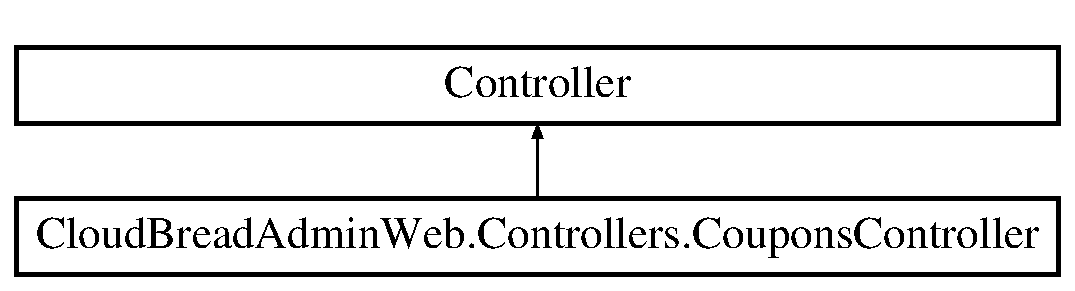
\includegraphics[height=2.000000cm]{a00071}
\end{center}
\end{figure}
\subsection*{Public Member Functions}
\begin{DoxyCompactItemize}
\item 
\hyperlink{a00068}{Coupon} {\bfseries Decrypt\+Result} (\hyperlink{a00068}{Coupon} item)\hypertarget{a00071_a0d78b9300023d4d572cccdf5fc272782}{}\label{a00071_a0d78b9300023d4d572cccdf5fc272782}

\item 
\hyperlink{a00068}{Coupon} {\bfseries Encrypt\+Result} (\hyperlink{a00068}{Coupon} item)\hypertarget{a00071_aeac3ad1dcd55d98bac7c27caee440ca4}{}\label{a00071_aeac3ad1dcd55d98bac7c27caee440ca4}

\item 
bool {\bfseries Check\+Session} ()\hypertarget{a00071_ae05fb87ce1e4b4a3b40c12edb26c2813}{}\label{a00071_ae05fb87ce1e4b4a3b40c12edb26c2813}

\item 
Action\+Result {\bfseries Index} (string search\+String, string Search\+Condition, string current\+Filter, int?page)\hypertarget{a00071_a17770c0afe56bfa23bb1feef7f0422f4}{}\label{a00071_a17770c0afe56bfa23bb1feef7f0422f4}

\item 
Action\+Result {\bfseries Details} (string id)\hypertarget{a00071_aba233e999b886228c0f32aeb09956e21}{}\label{a00071_aba233e999b886228c0f32aeb09956e21}

\item 
Action\+Result {\bfseries Create} ()\hypertarget{a00071_ab20df87a2e111f5132be283dfb6218b4}{}\label{a00071_ab20df87a2e111f5132be283dfb6218b4}

\item 
Action\+Result {\bfseries Create} (\mbox{[}Bind(Include=\char`\"{}Coupon\+ID,Coupon\+Category1,Coupon\+Category2,Coupon\+Category3,Item\+List\+ID,Item\+Count,Item\+Status,Target\+Group,Target\+OS,Target\+Device,Title,Content,s\+Col1,s\+Col2,s\+Col3,s\+Col4,s\+Col5,s\+Col6,s\+Col7,s\+Col8,s\+Col9,s\+Col10,Dupe\+YN,Order\+Number,Coupon\+Duration\+From,Coupon\+Duration\+To,Create\+Admin\+ID,Hide\+YN,Delete\+YN,Created\+At,Updated\+At,Data\+From\+Region,Data\+From\+Region\+DT\char`\"{})\mbox{]} Coupon coupon)\hypertarget{a00071_a09a4128160e5af4df99acba3cb1ac868}{}\label{a00071_a09a4128160e5af4df99acba3cb1ac868}

\item 
Action\+Result {\bfseries Edit} (string id)\hypertarget{a00071_a39373b6a5ca168ebb0a343e86d75f317}{}\label{a00071_a39373b6a5ca168ebb0a343e86d75f317}

\item 
Action\+Result {\bfseries Edit} (\mbox{[}Bind(Include=\char`\"{}Coupon\+ID,Coupon\+Category1,Coupon\+Category2,Coupon\+Category3,Item\+List\+ID,Item\+Count,Item\+Status,Target\+Group,Target\+OS,Target\+Device,Title,Content,s\+Col1,s\+Col2,s\+Col3,s\+Col4,s\+Col5,s\+Col6,s\+Col7,s\+Col8,s\+Col9,s\+Col10,Dupe\+YN,Order\+Number,Coupon\+Duration\+From,Coupon\+Duration\+To,Create\+Admin\+ID,Hide\+YN,Delete\+YN,Created\+At,Updated\+At,Data\+From\+Region,Data\+From\+Region\+DT\char`\"{})\mbox{]} Coupon coupon)\hypertarget{a00071_a415857b2d9920c1a983dcb7c5e0a8907}{}\label{a00071_a415857b2d9920c1a983dcb7c5e0a8907}

\item 
Action\+Result {\bfseries Delete} (string id)\hypertarget{a00071_afd61a6573b0021000457cdb396553d5f}{}\label{a00071_afd61a6573b0021000457cdb396553d5f}

\item 
Action\+Result {\bfseries Delete\+Confirmed} (string id)\hypertarget{a00071_a7e650ebeb88a7019d2f5b9bd1dea2a63}{}\label{a00071_a7e650ebeb88a7019d2f5b9bd1dea2a63}

\end{DoxyCompactItemize}
\subsection*{Protected Member Functions}
\begin{DoxyCompactItemize}
\item 
override void {\bfseries Dispose} (bool disposing)\hypertarget{a00071_a2a75abe700e452a7e64bbed73a835ad4}{}\label{a00071_a2a75abe700e452a7e64bbed73a835ad4}

\end{DoxyCompactItemize}


The documentation for this class was generated from the following file\+:\begin{DoxyCompactItemize}
\item 
C\+:/\+Users/dwkim/\+Documents/\+Git\+Hub/\+Cloud\+Bread/\+Cloud\+Bread\+Admin\+Web/\+Controllers/Coupons\+Controller.\+cs\end{DoxyCompactItemize}

\hypertarget{a00072}{}\section{Cloud\+Bread\+Lib.\+B\+A\+L.\+Crypto.\+Crypto Class Reference}
\label{a00072}\index{Cloud\+Bread\+Lib.\+B\+A\+L.\+Crypto.\+Crypto@{Cloud\+Bread\+Lib.\+B\+A\+L.\+Crypto.\+Crypto}}
\subsection*{Static Public Member Functions}
\begin{DoxyCompactItemize}
\item 
static string {\bfseries S\+H\+A512\+Hash\+Temp} (string Data)\hypertarget{a00072_a9e3bcd89fcf615211a3b130da12f303b}{}\label{a00072_a9e3bcd89fcf615211a3b130da12f303b}

\item 
static string {\bfseries S\+H\+A512\+Hash} (string Phrase)\hypertarget{a00072_a8fdf4f7ed36ccc7c4f06c24694be91a1}{}\label{a00072_a8fdf4f7ed36ccc7c4f06c24694be91a1}

\item 
static string {\bfseries M\+D5\+Hash} (string input)\hypertarget{a00072_a12caf024bb8996c2808bfc4885a9c9d4}{}\label{a00072_a12caf024bb8996c2808bfc4885a9c9d4}

\item 
static string {\bfseries A\+E\+S\+\_\+encrypt} (string Input, string key, string IV)\hypertarget{a00072_ae26608c3c151fe4b37af07553248156f}{}\label{a00072_ae26608c3c151fe4b37af07553248156f}

\item 
static string {\bfseries A\+E\+S\+\_\+decrypt} (string Input, string key, string IV)\hypertarget{a00072_a325a57ed3041b30afbe1f484f92d38be}{}\label{a00072_a325a57ed3041b30afbe1f484f92d38be}

\end{DoxyCompactItemize}


The documentation for this class was generated from the following file\+:\begin{DoxyCompactItemize}
\item 
C\+:/\+Users/dwkim/\+Documents/\+Git\+Hub/\+Cloud\+Bread/\+Cloud\+Bread\+Lib/\+B\+A\+L/Crypto.\+cs\end{DoxyCompactItemize}

\hypertarget{a00073}{}\section{Cloud\+Bread.\+Models.\+Com\+Udt\+Member\+Item\+Purchase\+Input\+Params Class Reference}
\label{a00073}\index{Cloud\+Bread.\+Models.\+Com\+Udt\+Member\+Item\+Purchase\+Input\+Params@{Cloud\+Bread.\+Models.\+Com\+Udt\+Member\+Item\+Purchase\+Input\+Params}}
\subsection*{Properties}
\begin{DoxyCompactItemize}
\item 
string {\bfseries Member\+Item\+Purchase\+ID}\hspace{0.3cm}{\ttfamily  \mbox{[}get, set\mbox{]}}\hypertarget{a00073_a943353068d05e690224036894504daa6}{}\label{a00073_a943353068d05e690224036894504daa6}

\item 
string {\bfseries Member\+ID}\hspace{0.3cm}{\ttfamily  \mbox{[}get, set\mbox{]}}\hypertarget{a00073_ae3215d6a99484082969d40f8ebbc1a5d}{}\label{a00073_ae3215d6a99484082969d40f8ebbc1a5d}

\item 
string {\bfseries Item\+List\+ID}\hspace{0.3cm}{\ttfamily  \mbox{[}get, set\mbox{]}}\hypertarget{a00073_abb89f9d2bbf6ba778914957102fa7f89}{}\label{a00073_abb89f9d2bbf6ba778914957102fa7f89}

\item 
string {\bfseries Purchase\+Quantity}\hspace{0.3cm}{\ttfamily  \mbox{[}get, set\mbox{]}}\hypertarget{a00073_a28a3868dc2f7634ca146f7be9e9b0975}{}\label{a00073_a28a3868dc2f7634ca146f7be9e9b0975}

\item 
string {\bfseries Purchase\+Price}\hspace{0.3cm}{\ttfamily  \mbox{[}get, set\mbox{]}}\hypertarget{a00073_a545c4a0df5cf5539637c608fe4b2eeba}{}\label{a00073_a545c4a0df5cf5539637c608fe4b2eeba}

\item 
string {\bfseries P\+Ginfo1}\hspace{0.3cm}{\ttfamily  \mbox{[}get, set\mbox{]}}\hypertarget{a00073_a2a8e4a8b41705a90470025652eed398c}{}\label{a00073_a2a8e4a8b41705a90470025652eed398c}

\item 
string {\bfseries P\+Ginfo2}\hspace{0.3cm}{\ttfamily  \mbox{[}get, set\mbox{]}}\hypertarget{a00073_acee949b0e2a71c9995bc85a451f8ac68}{}\label{a00073_acee949b0e2a71c9995bc85a451f8ac68}

\item 
string {\bfseries P\+Ginfo3}\hspace{0.3cm}{\ttfamily  \mbox{[}get, set\mbox{]}}\hypertarget{a00073_a593d3854e9fa1d3c1b4318aaa4beb61c}{}\label{a00073_a593d3854e9fa1d3c1b4318aaa4beb61c}

\item 
string {\bfseries P\+Ginfo4}\hspace{0.3cm}{\ttfamily  \mbox{[}get, set\mbox{]}}\hypertarget{a00073_a483a7fd8029616c12691db7cd6be940b}{}\label{a00073_a483a7fd8029616c12691db7cd6be940b}

\item 
string {\bfseries P\+Ginfo5}\hspace{0.3cm}{\ttfamily  \mbox{[}get, set\mbox{]}}\hypertarget{a00073_a0e657b86db26573d69a3e27940bca48f}{}\label{a00073_a0e657b86db26573d69a3e27940bca48f}

\item 
string {\bfseries Purchase\+Device\+ID}\hspace{0.3cm}{\ttfamily  \mbox{[}get, set\mbox{]}}\hypertarget{a00073_a020cdd466e9e8ec32039d78c8128c9ea}{}\label{a00073_a020cdd466e9e8ec32039d78c8128c9ea}

\item 
string {\bfseries Purchase\+Device\+I\+P\+Address}\hspace{0.3cm}{\ttfamily  \mbox{[}get, set\mbox{]}}\hypertarget{a00073_ae24aaff3eca28678c58fa857f39db3cf}{}\label{a00073_ae24aaff3eca28678c58fa857f39db3cf}

\item 
string {\bfseries Purchase\+Device\+M\+A\+C\+Address}\hspace{0.3cm}{\ttfamily  \mbox{[}get, set\mbox{]}}\hypertarget{a00073_a7e16603bcc56fd6cf8f4e5bb82863e27}{}\label{a00073_a7e16603bcc56fd6cf8f4e5bb82863e27}

\item 
string {\bfseries Purchase\+DT}\hspace{0.3cm}{\ttfamily  \mbox{[}get, set\mbox{]}}\hypertarget{a00073_a4b6584b5bf1607dec8b16241026f922d}{}\label{a00073_a4b6584b5bf1607dec8b16241026f922d}

\item 
string {\bfseries Purchase\+Cancel\+YN}\hspace{0.3cm}{\ttfamily  \mbox{[}get, set\mbox{]}}\hypertarget{a00073_aec07d32ffb97cb5432e1620fe3350364}{}\label{a00073_aec07d32ffb97cb5432e1620fe3350364}

\item 
string {\bfseries Purchase\+Cancel\+DT}\hspace{0.3cm}{\ttfamily  \mbox{[}get, set\mbox{]}}\hypertarget{a00073_a03c7e482a83c2e811149a8d22529ac95}{}\label{a00073_a03c7e482a83c2e811149a8d22529ac95}

\item 
string {\bfseries Purchase\+Canceling\+Status}\hspace{0.3cm}{\ttfamily  \mbox{[}get, set\mbox{]}}\hypertarget{a00073_a21184c7d62ce3a4819b9c4963ce04036}{}\label{a00073_a21184c7d62ce3a4819b9c4963ce04036}

\item 
string {\bfseries Purchase\+Cancel\+Returned\+Amount}\hspace{0.3cm}{\ttfamily  \mbox{[}get, set\mbox{]}}\hypertarget{a00073_ab12973c657ac52927a45cbafa05a19e8}{}\label{a00073_ab12973c657ac52927a45cbafa05a19e8}

\item 
string {\bfseries Purchase\+Cancel\+Device\+ID}\hspace{0.3cm}{\ttfamily  \mbox{[}get, set\mbox{]}}\hypertarget{a00073_aac739e612087c031a3e628328d72bbcc}{}\label{a00073_aac739e612087c031a3e628328d72bbcc}

\item 
string {\bfseries Purchase\+Cancel\+Device\+I\+P\+Address}\hspace{0.3cm}{\ttfamily  \mbox{[}get, set\mbox{]}}\hypertarget{a00073_ada74e758f4a9250de4f0c46d05b912e9}{}\label{a00073_ada74e758f4a9250de4f0c46d05b912e9}

\item 
string {\bfseries Purchase\+Cancel\+Device\+M\+A\+C\+Address}\hspace{0.3cm}{\ttfamily  \mbox{[}get, set\mbox{]}}\hypertarget{a00073_ae8b954773f323608d595e2a553667ea4}{}\label{a00073_ae8b954773f323608d595e2a553667ea4}

\item 
string {\bfseries s\+Col1}\hspace{0.3cm}{\ttfamily  \mbox{[}get, set\mbox{]}}\hypertarget{a00073_a7f0337fb0b932116543b57bc75bcc301}{}\label{a00073_a7f0337fb0b932116543b57bc75bcc301}

\item 
string {\bfseries s\+Col2}\hspace{0.3cm}{\ttfamily  \mbox{[}get, set\mbox{]}}\hypertarget{a00073_af2f729b454699ad31fc1f9b7a39ba85f}{}\label{a00073_af2f729b454699ad31fc1f9b7a39ba85f}

\item 
string {\bfseries s\+Col3}\hspace{0.3cm}{\ttfamily  \mbox{[}get, set\mbox{]}}\hypertarget{a00073_a056b4317d5a06a7b9299f0e25631c9c0}{}\label{a00073_a056b4317d5a06a7b9299f0e25631c9c0}

\item 
string {\bfseries s\+Col4}\hspace{0.3cm}{\ttfamily  \mbox{[}get, set\mbox{]}}\hypertarget{a00073_acbbd805f0a359313f261fad867a9084c}{}\label{a00073_acbbd805f0a359313f261fad867a9084c}

\item 
string {\bfseries s\+Col5}\hspace{0.3cm}{\ttfamily  \mbox{[}get, set\mbox{]}}\hypertarget{a00073_a2f90cb8ade6cb4c2987d38bef33027ba}{}\label{a00073_a2f90cb8ade6cb4c2987d38bef33027ba}

\item 
string {\bfseries s\+Col6}\hspace{0.3cm}{\ttfamily  \mbox{[}get, set\mbox{]}}\hypertarget{a00073_addc50cd0ac68519dd07abbb15e440116}{}\label{a00073_addc50cd0ac68519dd07abbb15e440116}

\item 
string {\bfseries s\+Col7}\hspace{0.3cm}{\ttfamily  \mbox{[}get, set\mbox{]}}\hypertarget{a00073_a44bb698b2432b6df73b2522ebe8addc0}{}\label{a00073_a44bb698b2432b6df73b2522ebe8addc0}

\item 
string {\bfseries s\+Col8}\hspace{0.3cm}{\ttfamily  \mbox{[}get, set\mbox{]}}\hypertarget{a00073_a5d17a2b89065237be0b94de178aefd0a}{}\label{a00073_a5d17a2b89065237be0b94de178aefd0a}

\item 
string {\bfseries s\+Col9}\hspace{0.3cm}{\ttfamily  \mbox{[}get, set\mbox{]}}\hypertarget{a00073_a7409d85e6fa74b7b2102b70d1a3e1d99}{}\label{a00073_a7409d85e6fa74b7b2102b70d1a3e1d99}

\item 
string {\bfseries s\+Col10}\hspace{0.3cm}{\ttfamily  \mbox{[}get, set\mbox{]}}\hypertarget{a00073_a449ee8fc07339f4ec96b8fb1fe0bf4a6}{}\label{a00073_a449ee8fc07339f4ec96b8fb1fe0bf4a6}

\item 
string {\bfseries token}\hspace{0.3cm}{\ttfamily  \mbox{[}get, set\mbox{]}}\hypertarget{a00073_a53ff6a1c275d689a107d6ed65289a912}{}\label{a00073_a53ff6a1c275d689a107d6ed65289a912}

\end{DoxyCompactItemize}


The documentation for this class was generated from the following file\+:\begin{DoxyCompactItemize}
\item 
C\+:/\+Users/dwkim/\+Documents/\+Git\+Hub/\+Cloud\+Bread/\+Models/Com\+Udt\+Member\+Item\+Purchase.\+cs\end{DoxyCompactItemize}

\hypertarget{a00074}{}\section{Cloud\+Bread.\+Models.\+Encrypted\+Data Class Reference}
\label{a00074}\index{Cloud\+Bread.\+Models.\+Encrypted\+Data@{Cloud\+Bread.\+Models.\+Encrypted\+Data}}
\subsection*{Properties}
\begin{DoxyCompactItemize}
\item 
string {\bfseries token}\hspace{0.3cm}{\ttfamily  \mbox{[}get, set\mbox{]}}\hypertarget{a00074_a6aebf9b968ebbdb57cfac4e0178ebf41}{}\label{a00074_a6aebf9b968ebbdb57cfac4e0178ebf41}

\end{DoxyCompactItemize}


The documentation for this class was generated from the following file\+:\begin{DoxyCompactItemize}
\item 
C\+:/\+Users/dwkim/\+Documents/\+Git\+Hub/\+Cloud\+Bread/\+Models/Encrypted\+Data.\+cs\end{DoxyCompactItemize}

\hypertarget{a00075}{}\section{Cloud\+Bread\+Admin\+Web.\+Models.\+External\+Login\+Confirmation\+View\+Model Class Reference}
\label{a00075}\index{Cloud\+Bread\+Admin\+Web.\+Models.\+External\+Login\+Confirmation\+View\+Model@{Cloud\+Bread\+Admin\+Web.\+Models.\+External\+Login\+Confirmation\+View\+Model}}
\subsection*{Properties}
\begin{DoxyCompactItemize}
\item 
string {\bfseries Email}\hspace{0.3cm}{\ttfamily  \mbox{[}get, set\mbox{]}}\hypertarget{a00075_a2082e7aae001a613bf12bb05e0e52eea}{}\label{a00075_a2082e7aae001a613bf12bb05e0e52eea}

\end{DoxyCompactItemize}


The documentation for this class was generated from the following file\+:\begin{DoxyCompactItemize}
\item 
C\+:/\+Users/dwkim/\+Documents/\+Git\+Hub/\+Cloud\+Bread/\+Cloud\+Bread\+Admin\+Web/\+Models/Account\+View\+Models.\+cs\end{DoxyCompactItemize}

\hypertarget{a00076}{}\section{Cloud\+Bread.\+Controllers.\+C\+B\+Rank\+Controller.\+Input\+Params Class Reference}
\label{a00076}\index{Cloud\+Bread.\+Controllers.\+C\+B\+Rank\+Controller.\+Input\+Params@{Cloud\+Bread.\+Controllers.\+C\+B\+Rank\+Controller.\+Input\+Params}}
\subsection*{Properties}
\begin{DoxyCompactItemize}
\item 
string {\bfseries sid}\hspace{0.3cm}{\ttfamily  \mbox{[}get, set\mbox{]}}\hypertarget{a00076_a4c7c042b79f056fd99dc06c53a27ce84}{}\label{a00076_a4c7c042b79f056fd99dc06c53a27ce84}

\item 
double {\bfseries point}\hspace{0.3cm}{\ttfamily  \mbox{[}get, set\mbox{]}}\hypertarget{a00076_a8eb10e4dbcdc60810081039ce689983b}{}\label{a00076_a8eb10e4dbcdc60810081039ce689983b}

\end{DoxyCompactItemize}


The documentation for this class was generated from the following file\+:\begin{DoxyCompactItemize}
\item 
C\+:/\+Users/dwkim/\+Documents/\+Git\+Hub/\+Cloud\+Bread/\+Controllers/C\+B\+Rank\+Controller.\+cs\end{DoxyCompactItemize}

\hypertarget{a00077}{}\section{Cloud\+Bread\+Admin\+Web.\+Models.\+Factor\+View\+Model Class Reference}
\label{a00077}\index{Cloud\+Bread\+Admin\+Web.\+Models.\+Factor\+View\+Model@{Cloud\+Bread\+Admin\+Web.\+Models.\+Factor\+View\+Model}}
\subsection*{Properties}
\begin{DoxyCompactItemize}
\item 
string {\bfseries Purpose}\hspace{0.3cm}{\ttfamily  \mbox{[}get, set\mbox{]}}\hypertarget{a00077_aeae54cc6159853dbd9931d76366b9124}{}\label{a00077_aeae54cc6159853dbd9931d76366b9124}

\end{DoxyCompactItemize}


The documentation for this class was generated from the following file\+:\begin{DoxyCompactItemize}
\item 
C\+:/\+Users/dwkim/\+Documents/\+Git\+Hub/\+Cloud\+Bread/\+Cloud\+Bread\+Admin\+Web/\+Models/Manage\+View\+Models.\+cs\end{DoxyCompactItemize}

\hypertarget{a00078}{}\section{Logger.\+Logging.\+Logging Class Reference}
\label{a00078}\index{Logger.\+Logging.\+Logging@{Logger.\+Logging.\+Logging}}
\subsection*{Classes}
\begin{DoxyCompactItemize}
\item 
class \hyperlink{a00008}{C\+B\+A\+T\+S\+Message\+Entity}
\begin{DoxyCompactList}\small\item\em Entity class for log structure -\/ including A\+TS ~\newline
. \end{DoxyCompactList}\item 
class \hyperlink{a00028}{C\+B\+Loggers}
\begin{DoxyCompactList}\small\item\em Processing \hyperlink{a00217}{Cloud\+Bread} log related task class. ~\newline
. \end{DoxyCompactList}\end{DoxyCompactItemize}
\subsection*{Static Public Member Functions}
\begin{DoxyCompactItemize}
\item 
static bool \hyperlink{a00078_ab9ee47be781439bd81b8546287e6c48c}{Run\+Log} (\hyperlink{a00028}{C\+B\+Loggers} message)
\begin{DoxyCompactList}\small\item\em Save log task processor. ~\newline
. \end{DoxyCompactList}\end{DoxyCompactItemize}


\subsection{Member Function Documentation}
\index{Logger\+::\+Logging\+::\+Logging@{Logger\+::\+Logging\+::\+Logging}!Run\+Log@{Run\+Log}}
\index{Run\+Log@{Run\+Log}!Logger\+::\+Logging\+::\+Logging@{Logger\+::\+Logging\+::\+Logging}}
\subsubsection[{\texorpdfstring{Run\+Log(\+C\+B\+Loggers message)}{RunLog(CBLoggers message)}}]{\setlength{\rightskip}{0pt plus 5cm}static bool Logger.\+Logging.\+Logging.\+Run\+Log (
\begin{DoxyParamCaption}
\item[{{\bf C\+B\+Loggers}}]{message}
\end{DoxyParamCaption}
)\hspace{0.3cm}{\ttfamily [static]}}\hypertarget{a00078_ab9ee47be781439bd81b8546287e6c48c}{}\label{a00078_ab9ee47be781439bd81b8546287e6c48c}


Save log task processor. ~\newline
. 

in case of non-\/member triggered job

critical error case, save in A\+TS Cloud\+Bread\+Error\+Log

Save error log on Azure Table Storage

Azure Table Storage connection retry policy

Catch fail to log on database. Most case database connection or login fail issue.

Regarding to web.\+config logger settting, save logs on specific storage

Save log on S\+QL

Database connection retry policy

Save log on Azure Table Storage

Azure Table Storage connection retry policy

Save log on Azure Queue Storage

Azure Queue Storage connection retry policy

must be lower case

todolist -\/ save log on Azure Redis Cache yyyymmdd\+:memberid\+:\+Controller\+:G\+U\+ID

case do nothing

catch save log error here. 

The documentation for this class was generated from the following file\+:\begin{DoxyCompactItemize}
\item 
C\+:/\+Users/dwkim/\+Documents/\+Git\+Hub/\+Cloud\+Bread/C\+B\+Loggers.\+cs\end{DoxyCompactItemize}

\hypertarget{a00079}{}\section{Cloud\+Bread\+Admin\+Web.\+Models.\+Forgot\+Password\+View\+Model Class Reference}
\label{a00079}\index{Cloud\+Bread\+Admin\+Web.\+Models.\+Forgot\+Password\+View\+Model@{Cloud\+Bread\+Admin\+Web.\+Models.\+Forgot\+Password\+View\+Model}}
\subsection*{Properties}
\begin{DoxyCompactItemize}
\item 
string {\bfseries Email}\hspace{0.3cm}{\ttfamily  \mbox{[}get, set\mbox{]}}\hypertarget{a00079_af77b60581e2d17267d66cef30a60a6c1}{}\label{a00079_af77b60581e2d17267d66cef30a60a6c1}

\end{DoxyCompactItemize}


The documentation for this class was generated from the following file\+:\begin{DoxyCompactItemize}
\item 
C\+:/\+Users/dwkim/\+Documents/\+Git\+Hub/\+Cloud\+Bread/\+Cloud\+Bread\+Admin\+Web/\+Models/Account\+View\+Models.\+cs\end{DoxyCompactItemize}

\hypertarget{a00080}{}\section{Cloud\+Bread.\+Models.\+Mobile\+Service\+Context Class Reference}
\label{a00080}\index{Cloud\+Bread.\+Models.\+Mobile\+Service\+Context@{Cloud\+Bread.\+Models.\+Mobile\+Service\+Context}}
Inheritance diagram for Cloud\+Bread.\+Models.\+Mobile\+Service\+Context\+:\begin{figure}[H]
\begin{center}
\leavevmode
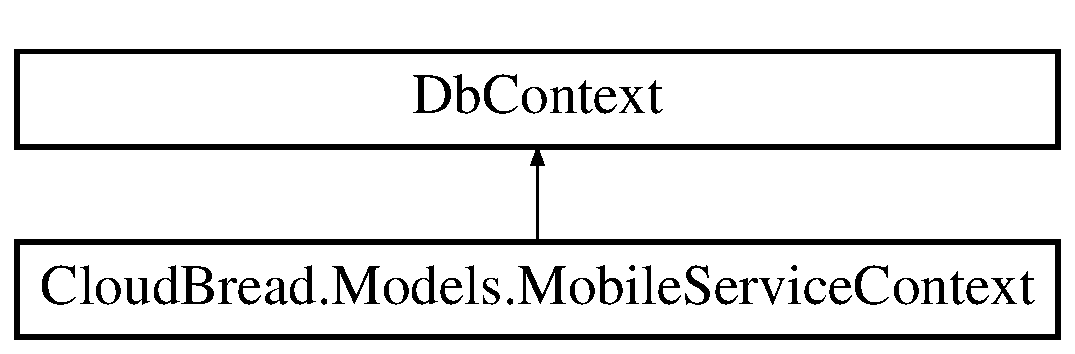
\includegraphics[height=2.000000cm]{a00080}
\end{center}
\end{figure}
\subsection*{Protected Member Functions}
\begin{DoxyCompactItemize}
\item 
override void {\bfseries On\+Model\+Creating} (Db\+Model\+Builder model\+Builder)\hypertarget{a00080_a98c14d9e5b9403754d5b717f672ed77f}{}\label{a00080_a98c14d9e5b9403754d5b717f672ed77f}

\end{DoxyCompactItemize}
\subsection*{Properties}
\begin{DoxyCompactItemize}
\item 
Db\+Set$<$ \hyperlink{a00106}{Todo\+Item} $>$ {\bfseries Todo\+Items}\hspace{0.3cm}{\ttfamily  \mbox{[}get, set\mbox{]}}\hypertarget{a00080_aa02a40c8717cd4fa77923470c670f56d}{}\label{a00080_aa02a40c8717cd4fa77923470c670f56d}

\end{DoxyCompactItemize}


The documentation for this class was generated from the following file\+:\begin{DoxyCompactItemize}
\item 
C\+:/\+Users/dwkim/\+Documents/\+Git\+Hub/\+Cloud\+Bread/\+Models/Mobile\+Service\+Context.\+cs\end{DoxyCompactItemize}

\hypertarget{a00081}{}\section{Cloud\+Bread\+Admin\+Web.\+Game\+Event\+Member Class Reference}
\label{a00081}\index{Cloud\+Bread\+Admin\+Web.\+Game\+Event\+Member@{Cloud\+Bread\+Admin\+Web.\+Game\+Event\+Member}}
\subsection*{Properties}
\begin{DoxyCompactItemize}
\item 
string {\bfseries Game\+Event\+Member\+ID}\hspace{0.3cm}{\ttfamily  \mbox{[}get, set\mbox{]}}\hypertarget{a00081_a651d1629ec9958bbd1c33f4c4e6c97d4}{}\label{a00081_a651d1629ec9958bbd1c33f4c4e6c97d4}

\item 
string {\bfseries event\+ID}\hspace{0.3cm}{\ttfamily  \mbox{[}get, set\mbox{]}}\hypertarget{a00081_a574e5d67df647eba163c9a1bc319c77f}{}\label{a00081_a574e5d67df647eba163c9a1bc319c77f}

\item 
string {\bfseries Member\+ID}\hspace{0.3cm}{\ttfamily  \mbox{[}get, set\mbox{]}}\hypertarget{a00081_a085b6a4f56c6ed2ec95fd1c35bf34d67}{}\label{a00081_a085b6a4f56c6ed2ec95fd1c35bf34d67}

\item 
string {\bfseries s\+Col1}\hspace{0.3cm}{\ttfamily  \mbox{[}get, set\mbox{]}}\hypertarget{a00081_aaeb96916c15c51b0ad086f9f38550bc6}{}\label{a00081_aaeb96916c15c51b0ad086f9f38550bc6}

\item 
string {\bfseries s\+Col2}\hspace{0.3cm}{\ttfamily  \mbox{[}get, set\mbox{]}}\hypertarget{a00081_ac755b234cb5cba0faab04ed6ffe236f8}{}\label{a00081_ac755b234cb5cba0faab04ed6ffe236f8}

\item 
string {\bfseries s\+Col3}\hspace{0.3cm}{\ttfamily  \mbox{[}get, set\mbox{]}}\hypertarget{a00081_a946e643c56952399557c41b4b397f2c7}{}\label{a00081_a946e643c56952399557c41b4b397f2c7}

\item 
string {\bfseries s\+Col4}\hspace{0.3cm}{\ttfamily  \mbox{[}get, set\mbox{]}}\hypertarget{a00081_a04b6a857a76309dbf8a5e682e4d85f17}{}\label{a00081_a04b6a857a76309dbf8a5e682e4d85f17}

\item 
string {\bfseries s\+Col5}\hspace{0.3cm}{\ttfamily  \mbox{[}get, set\mbox{]}}\hypertarget{a00081_a4831173aa3ee5a18e60b0dc4ddd2128d}{}\label{a00081_a4831173aa3ee5a18e60b0dc4ddd2128d}

\item 
string {\bfseries s\+Col6}\hspace{0.3cm}{\ttfamily  \mbox{[}get, set\mbox{]}}\hypertarget{a00081_a63407aa40663ef4657c194443a2b9dcd}{}\label{a00081_a63407aa40663ef4657c194443a2b9dcd}

\item 
string {\bfseries s\+Col7}\hspace{0.3cm}{\ttfamily  \mbox{[}get, set\mbox{]}}\hypertarget{a00081_ae8370999b39e80badbc6228f52dac161}{}\label{a00081_ae8370999b39e80badbc6228f52dac161}

\item 
string {\bfseries s\+Col8}\hspace{0.3cm}{\ttfamily  \mbox{[}get, set\mbox{]}}\hypertarget{a00081_a1fd14fb9cd552f6d5787773f0bd84a6e}{}\label{a00081_a1fd14fb9cd552f6d5787773f0bd84a6e}

\item 
string {\bfseries s\+Col9}\hspace{0.3cm}{\ttfamily  \mbox{[}get, set\mbox{]}}\hypertarget{a00081_ae1958ee4df4844a3c8bdd5ffcd96099b}{}\label{a00081_ae1958ee4df4844a3c8bdd5ffcd96099b}

\item 
string {\bfseries s\+Col10}\hspace{0.3cm}{\ttfamily  \mbox{[}get, set\mbox{]}}\hypertarget{a00081_ac6da501dc9510002a2be6206d876d35f}{}\label{a00081_ac6da501dc9510002a2be6206d876d35f}

\item 
string {\bfseries Hide\+YN}\hspace{0.3cm}{\ttfamily  \mbox{[}get, set\mbox{]}}\hypertarget{a00081_a795f7139d3c181037afa8b127faa4001}{}\label{a00081_a795f7139d3c181037afa8b127faa4001}

\item 
string {\bfseries Delete\+YN}\hspace{0.3cm}{\ttfamily  \mbox{[}get, set\mbox{]}}\hypertarget{a00081_a60a9bb0abb52bcd60b581a62545e5f0d}{}\label{a00081_a60a9bb0abb52bcd60b581a62545e5f0d}

\item 
System.\+Date\+Time\+Offset {\bfseries Created\+At}\hspace{0.3cm}{\ttfamily  \mbox{[}get, set\mbox{]}}\hypertarget{a00081_a7690363ec31a6a47d85bb08e7cc571ed}{}\label{a00081_a7690363ec31a6a47d85bb08e7cc571ed}

\item 
System.\+Date\+Time\+Offset {\bfseries Updated\+At}\hspace{0.3cm}{\ttfamily  \mbox{[}get, set\mbox{]}}\hypertarget{a00081_afdda990dd3e874e25b4574fe37e41e0e}{}\label{a00081_afdda990dd3e874e25b4574fe37e41e0e}

\item 
string {\bfseries Data\+From\+Region}\hspace{0.3cm}{\ttfamily  \mbox{[}get, set\mbox{]}}\hypertarget{a00081_aeaa6ff575a463307fb51e68d15b2107c}{}\label{a00081_aeaa6ff575a463307fb51e68d15b2107c}

\item 
System.\+Date\+Time\+Offset {\bfseries Data\+From\+Region\+DT}\hspace{0.3cm}{\ttfamily  \mbox{[}get, set\mbox{]}}\hypertarget{a00081_a939b81b2f0526959256daba5a33bd924}{}\label{a00081_a939b81b2f0526959256daba5a33bd924}

\item 
virtual \hyperlink{a00083}{Game\+Events} {\bfseries Game\+Events}\hspace{0.3cm}{\ttfamily  \mbox{[}get, set\mbox{]}}\hypertarget{a00081_ae56ccac6b760bafb3a2bffadeb7afd9f}{}\label{a00081_ae56ccac6b760bafb3a2bffadeb7afd9f}

\item 
virtual \hyperlink{a00145}{Members} {\bfseries Members}\hspace{0.3cm}{\ttfamily  \mbox{[}get, set\mbox{]}}\hypertarget{a00081_a9bb13544fabf664de6ae66a867301000}{}\label{a00081_a9bb13544fabf664de6ae66a867301000}

\end{DoxyCompactItemize}


The documentation for this class was generated from the following files\+:\begin{DoxyCompactItemize}
\item 
C\+:/\+Users/dwkim/\+Documents/\+Git\+Hub/\+Cloud\+Bread/\+Cloud\+Bread\+Admin\+Web/Game\+Event\+Member.\+cs\item 
C\+:/\+Users/dwkim/\+Documents/\+Git\+Hub/\+Cloud\+Bread/\+Cloud\+Bread\+Admin\+Web/\+Models/Data\+Annotation\+Meta\+Model.\+cs\end{DoxyCompactItemize}

\hypertarget{a00082}{}\section{Cloud\+Bread.\+Controllers.\+C\+B\+Socket\+Auth\+Controller.\+Payload Class Reference}
\label{a00082}\index{Cloud\+Bread.\+Controllers.\+C\+B\+Socket\+Auth\+Controller.\+Payload@{Cloud\+Bread.\+Controllers.\+C\+B\+Socket\+Auth\+Controller.\+Payload}}
\subsection*{Properties}
\begin{DoxyCompactItemize}
\item 
string {\bfseries guid}\hspace{0.3cm}{\ttfamily  \mbox{[}get, set\mbox{]}}\hypertarget{a00082_aa2de66cdffd308627d2c00ef0514d560}{}\label{a00082_aa2de66cdffd308627d2c00ef0514d560}

\item 
string {\bfseries sid}\hspace{0.3cm}{\ttfamily  \mbox{[}get, set\mbox{]}}\hypertarget{a00082_af7bc9e4d78c4087c82a2aab7c547868d}{}\label{a00082_af7bc9e4d78c4087c82a2aab7c547868d}

\item 
string \hyperlink{a00082_a8578f804b87fd27135c1d3f4712aa7e0}{gen\+Date\+U\+TC}\hspace{0.3cm}{\ttfamily  \mbox{[}get, set\mbox{]}}
\end{DoxyCompactItemize}


\subsection{Property Documentation}
\index{Cloud\+Bread\+::\+Controllers\+::\+C\+B\+Socket\+Auth\+Controller\+::\+Payload@{Cloud\+Bread\+::\+Controllers\+::\+C\+B\+Socket\+Auth\+Controller\+::\+Payload}!gen\+Date\+U\+TC@{gen\+Date\+U\+TC}}
\index{gen\+Date\+U\+TC@{gen\+Date\+U\+TC}!Cloud\+Bread\+::\+Controllers\+::\+C\+B\+Socket\+Auth\+Controller\+::\+Payload@{Cloud\+Bread\+::\+Controllers\+::\+C\+B\+Socket\+Auth\+Controller\+::\+Payload}}
\subsubsection[{\texorpdfstring{gen\+Date\+U\+TC}{genDateUTC}}]{\setlength{\rightskip}{0pt plus 5cm}string Cloud\+Bread.\+Controllers.\+C\+B\+Socket\+Auth\+Controller.\+Payload.\+gen\+Date\+U\+TC\hspace{0.3cm}{\ttfamily [get]}, {\ttfamily [set]}}\hypertarget{a00082_a8578f804b87fd27135c1d3f4712aa7e0}{}\label{a00082_a8578f804b87fd27135c1d3f4712aa7e0}
\begin{DoxyRefDesc}{Todo}
\item[\hyperlink{a00001__todo000017}{Todo}]do not show this value client \end{DoxyRefDesc}


The documentation for this class was generated from the following file\+:\begin{DoxyCompactItemize}
\item 
C\+:/\+Users/dwkim/\+Documents/\+Git\+Hub/\+Cloud\+Bread/\+Controllers/\hyperlink{a00153}{C\+B\+Socket\+Auth\+Controller.\+cs}\end{DoxyCompactItemize}

\hypertarget{a00083}{}\section{Cloud\+Bread.\+Controllers.\+Ping\+Controller Class Reference}
\label{a00083}\index{Cloud\+Bread.\+Controllers.\+Ping\+Controller@{Cloud\+Bread.\+Controllers.\+Ping\+Controller}}
Inheritance diagram for Cloud\+Bread.\+Controllers.\+Ping\+Controller\+:\begin{figure}[H]
\begin{center}
\leavevmode
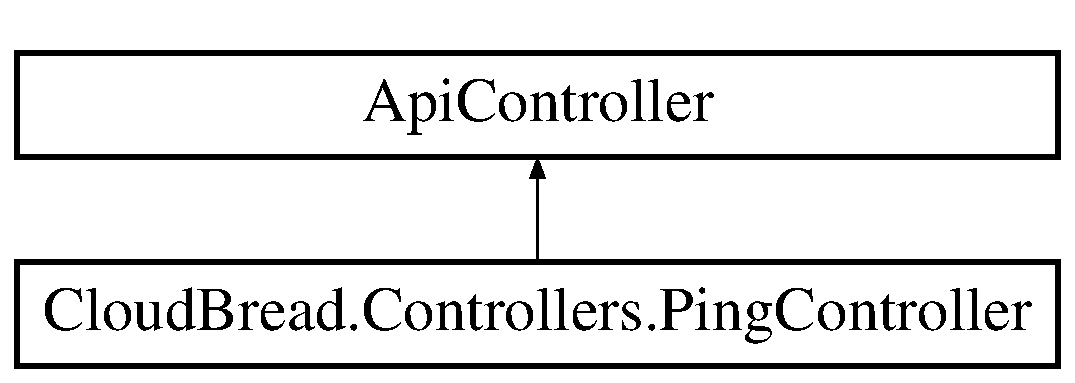
\includegraphics[height=2.000000cm]{a00083}
\end{center}
\end{figure}
\subsection*{Public Member Functions}
\begin{DoxyCompactItemize}
\item 
string \hyperlink{a00083_a522bb782fa548bc7cc0596da2332dab4}{Get} ()\hypertarget{a00083_a522bb782fa548bc7cc0596da2332dab4}{}\label{a00083_a522bb782fa548bc7cc0596da2332dab4}

\begin{DoxyCompactList}\small\item\em G\+ET api/ping -\/ return ping test string. \end{DoxyCompactList}\item 
string {\bfseries Post} ()\hypertarget{a00083_a55bcbbd6f8f97d1b9f7b480f5a3c754a}{}\label{a00083_a55bcbbd6f8f97d1b9f7b480f5a3c754a}

\end{DoxyCompactItemize}


The documentation for this class was generated from the following file\+:\begin{DoxyCompactItemize}
\item 
C\+:/\+Users/dwkim/\+Documents/\+Git\+Hub/\+Cloud\+Bread/\+Controllers/\hyperlink{a00163}{Ping\+Controller.\+cs}\end{DoxyCompactItemize}

\hypertarget{a00084}{}\section{Cloud\+Bread\+Admin\+Web.\+Controllers.\+Game\+Events\+Controller Class Reference}
\label{a00084}\index{Cloud\+Bread\+Admin\+Web.\+Controllers.\+Game\+Events\+Controller@{Cloud\+Bread\+Admin\+Web.\+Controllers.\+Game\+Events\+Controller}}
Inheritance diagram for Cloud\+Bread\+Admin\+Web.\+Controllers.\+Game\+Events\+Controller\+:\begin{figure}[H]
\begin{center}
\leavevmode
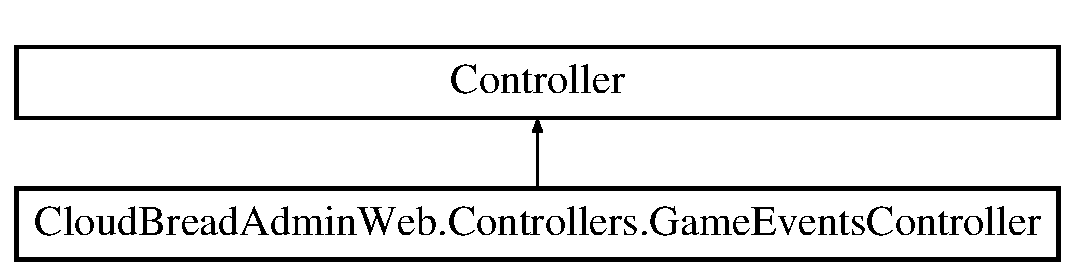
\includegraphics[height=2.000000cm]{a00084}
\end{center}
\end{figure}
\subsection*{Public Member Functions}
\begin{DoxyCompactItemize}
\item 
\hyperlink{a00083}{Game\+Events} {\bfseries Decrypt\+Result} (\hyperlink{a00083}{Game\+Events} item)\hypertarget{a00084_aa998d6457a3edb40fc2ac5eb3d7217bd}{}\label{a00084_aa998d6457a3edb40fc2ac5eb3d7217bd}

\item 
\hyperlink{a00083}{Game\+Events} {\bfseries Encrypt\+Result} (\hyperlink{a00083}{Game\+Events} item)\hypertarget{a00084_ae132069bf87b71cf7074deae4d1b381c}{}\label{a00084_ae132069bf87b71cf7074deae4d1b381c}

\item 
bool {\bfseries Check\+Session} ()\hypertarget{a00084_a6716950665e3ed8eef8addbc65413251}{}\label{a00084_a6716950665e3ed8eef8addbc65413251}

\item 
Action\+Result {\bfseries Index} (string search\+String, string Search\+Condition, string current\+Filter, int?page)\hypertarget{a00084_a5d2c29c4fad527acc40b52078e2eec07}{}\label{a00084_a5d2c29c4fad527acc40b52078e2eec07}

\item 
Action\+Result {\bfseries Details} (string id)\hypertarget{a00084_a8233163d3d36932f0c8b28940958aaf5}{}\label{a00084_a8233163d3d36932f0c8b28940958aaf5}

\item 
Action\+Result {\bfseries Create} ()\hypertarget{a00084_a623aedeac0dbef7fb7c8cf25208abeef}{}\label{a00084_a623aedeac0dbef7fb7c8cf25208abeef}

\item 
Action\+Result {\bfseries Create} (\mbox{[}Bind(Include=\char`\"{}Game\+Event\+ID,Event\+Category1,Event\+Category2,Event\+Category3,Item\+List\+ID,Item\+Count,Itemstatus,Target\+Group,Target\+OS,Target\+Device,Event\+Image\+Link,Title,Content,s\+Col1,s\+Col2,s\+Col3,s\+Col4,s\+Col5,s\+Col6,s\+Col7,s\+Col8,s\+Col9,s\+Col10,Event\+Duration\+From,Event\+Duration\+To,Order\+Number,Create\+Admin\+ID,Hide\+YN,Delete\+YN,Created\+At,Updated\+At,Data\+From\+Region,Data\+From\+Region\+DT\char`\"{})\mbox{]} Game\+Events game\+Events)\hypertarget{a00084_ac76e75b14047bcdb69cc784cbdfa5993}{}\label{a00084_ac76e75b14047bcdb69cc784cbdfa5993}

\item 
Action\+Result {\bfseries Edit} (string id)\hypertarget{a00084_a0b743baa7e1c50e34095856eb2eea3a9}{}\label{a00084_a0b743baa7e1c50e34095856eb2eea3a9}

\item 
Action\+Result {\bfseries Edit} (\mbox{[}Bind(Include=\char`\"{}Game\+Event\+ID,Event\+Category1,Event\+Category2,Event\+Category3,Item\+List\+ID,Item\+Count,Itemstatus,Target\+Group,Target\+OS,Target\+Device,Event\+Image\+Link,Title,Content,s\+Col1,s\+Col2,s\+Col3,s\+Col4,s\+Col5,s\+Col6,s\+Col7,s\+Col8,s\+Col9,s\+Col10,Event\+Duration\+From,Event\+Duration\+To,Order\+Number,Create\+Admin\+ID,Hide\+YN,Delete\+YN,Created\+At,Updated\+At,Data\+From\+Region,Data\+From\+Region\+DT\char`\"{})\mbox{]} Game\+Events game\+Events)\hypertarget{a00084_a8cf4442b12f5ca4f9d04d68d82a530d7}{}\label{a00084_a8cf4442b12f5ca4f9d04d68d82a530d7}

\item 
Action\+Result {\bfseries Delete} (string id)\hypertarget{a00084_a38e12ff4ecb98405ed9544bdc413aee0}{}\label{a00084_a38e12ff4ecb98405ed9544bdc413aee0}

\item 
Action\+Result {\bfseries Delete\+Confirmed} (string id)\hypertarget{a00084_a6d8873e561d1d02453ae2e6859e46692}{}\label{a00084_a6d8873e561d1d02453ae2e6859e46692}

\end{DoxyCompactItemize}
\subsection*{Protected Member Functions}
\begin{DoxyCompactItemize}
\item 
override void {\bfseries Dispose} (bool disposing)\hypertarget{a00084_a682b5d4169ab1b930a51b78f156a5ee5}{}\label{a00084_a682b5d4169ab1b930a51b78f156a5ee5}

\end{DoxyCompactItemize}


The documentation for this class was generated from the following file\+:\begin{DoxyCompactItemize}
\item 
C\+:/\+Users/dwkim/\+Documents/\+Git\+Hub/\+Cloud\+Bread/\+Cloud\+Bread\+Admin\+Web/\+Controllers/Game\+Events\+Controller.\+cs\end{DoxyCompactItemize}

\hypertarget{a00085}{}\section{Cloud\+Bread\+Lib.\+D\+A\+L.\+Generate\+C\+B\+Q.\+Generate\+C\+BQ Class Reference}
\label{a00085}\index{Cloud\+Bread\+Lib.\+D\+A\+L.\+Generate\+C\+B\+Q.\+Generate\+C\+BQ@{Cloud\+Bread\+Lib.\+D\+A\+L.\+Generate\+C\+B\+Q.\+Generate\+C\+BQ}}
\subsection*{Static Public Attributes}
\begin{DoxyCompactItemize}
\item 
static string {\bfseries Json} = @\char`\"{}\{\textquotesingle{}s\textquotesingle{}\+:\textquotesingle{}set nocount on\textquotesingle{},\textquotesingle{}bt\textquotesingle{}\+:\textquotesingle{}begin tran\textquotesingle{},\textquotesingle{}q\textquotesingle{}\+:\mbox{[}\{\textquotesingle{}qt\textquotesingle{}\+:\textquotesingle{}i\textquotesingle{},\textquotesingle{}t\textquotesingle{}\+:\textquotesingle{}member\textquotesingle{},\textquotesingle{}c\textquotesingle{}\+:\textquotesingle{}member.\+memberid, member.\+membername\textquotesingle{},\textquotesingle{}v\textquotesingle{}\+:\textquotesingle{}1, \textbackslash{}\textquotesingle{}구름빵\textbackslash{}\textquotesingle{}\textquotesingle{},\textquotesingle{}w\textquotesingle{}\+:\textquotesingle{}\textquotesingle{},\textquotesingle{}o\textquotesingle{}\+:\textquotesingle{}\textquotesingle{},\textquotesingle{}j\textquotesingle{}\+:\textquotesingle{}\textquotesingle{},\textquotesingle{}nl\textquotesingle{}\+:\textquotesingle{}\textquotesingle{}\},\{\textquotesingle{}qt\textquotesingle{}\+:\textquotesingle{}u\textquotesingle{},\textquotesingle{}t\textquotesingle{}\+:\textquotesingle{}member\textquotesingle{},\textquotesingle{}c\textquotesingle{}\+:\textquotesingle{}member.\+memberid, member.\+membername\textquotesingle{},\textquotesingle{}v\textquotesingle{}\+:\textquotesingle{}2, \textbackslash{}\textquotesingle{}프로젝트\textbackslash{}\textquotesingle{}\textquotesingle{},\textquotesingle{}w\textquotesingle{}\+:\textquotesingle{}member.\+memberid = 1\textquotesingle{},\textquotesingle{}o\textquotesingle{}\+:\textquotesingle{}\textquotesingle{},\textquotesingle{}j\textquotesingle{}\+:\textquotesingle{}\textquotesingle{},\textquotesingle{}nl\textquotesingle{}\+:\textquotesingle{}\textquotesingle{}\},\{\textquotesingle{}qt\textquotesingle{}\+:\textquotesingle{}d\textquotesingle{},\textquotesingle{}t\textquotesingle{}\+:\textquotesingle{}member\textquotesingle{},\textquotesingle{}c\textquotesingle{}\+:\textquotesingle{}\textquotesingle{},\textquotesingle{}v\textquotesingle{}\+:\textquotesingle{}\textquotesingle{},\textquotesingle{}w\textquotesingle{}\+:\textquotesingle{}member.\+memberid=1 and member.\+membername = \textbackslash{}\textquotesingle{}프로젝트\textbackslash{}\textquotesingle{}\textquotesingle{},\textquotesingle{}o\textquotesingle{}\+:\textquotesingle{}\textquotesingle{},\textquotesingle{}j\textquotesingle{}\+:\textquotesingle{}\textquotesingle{},\textquotesingle{}nl\textquotesingle{}\+:\textquotesingle{}\textquotesingle{}\},\{\textquotesingle{}qt\textquotesingle{}\+:\textquotesingle{}s\textquotesingle{},\textquotesingle{}t\textquotesingle{}\+:\textquotesingle{}member\textquotesingle{},\textquotesingle{}c\textquotesingle{}\+:\textquotesingle{}member.\+memberid, member.\+membername\textquotesingle{},\textquotesingle{}v\textquotesingle{}\+:\textquotesingle{}\textquotesingle{},\textquotesingle{}w\textquotesingle{}\+:\textquotesingle{}member.\+memberid=1, member.\+membername like \textbackslash{}\textquotesingle{}회원\textbackslash{}\textquotesingle{}\textquotesingle{},\textquotesingle{}o\textquotesingle{}\+:\textquotesingle{}orderby\textquotesingle{},\textquotesingle{}j\textquotesingle{}\+:\textquotesingle{}\textquotesingle{},\textquotesingle{}nl\textquotesingle{}\+:\textquotesingle{}\textquotesingle{}\},\mbox{]},\textquotesingle{}ct\textquotesingle{}\+:\textquotesingle{}\textquotesingle{}\}\char`\"{}\hypertarget{a00085_a91fcb156883a57b49b6766b1832f9d10}{}\label{a00085_a91fcb156883a57b49b6766b1832f9d10}

\end{DoxyCompactItemize}


The documentation for this class was generated from the following file\+:\begin{DoxyCompactItemize}
\item 
C\+:/\+Users/dwkim/\+Documents/\+Git\+Hub/\+Cloud\+Bread/\+Cloud\+Bread\+Lib/\+D\+A\+L/Generate\+C\+B\+Q.\+cs\end{DoxyCompactItemize}

\hypertarget{a00086}{}\section{Cloud\+Bread\+Admin\+Web.\+Gift\+Depositories Class Reference}
\label{a00086}\index{Cloud\+Bread\+Admin\+Web.\+Gift\+Depositories@{Cloud\+Bread\+Admin\+Web.\+Gift\+Depositories}}
\subsection*{Properties}
\begin{DoxyCompactItemize}
\item 
string {\bfseries Gift\+Depository\+ID}\hspace{0.3cm}{\ttfamily  \mbox{[}get, set\mbox{]}}\hypertarget{a00086_a76c49c1714a8fa79c994317493ce4af4}{}\label{a00086_a76c49c1714a8fa79c994317493ce4af4}

\item 
string {\bfseries Item\+List\+ID}\hspace{0.3cm}{\ttfamily  \mbox{[}get, set\mbox{]}}\hypertarget{a00086_ad177025b7cad26e9b84015cf6d018c2a}{}\label{a00086_ad177025b7cad26e9b84015cf6d018c2a}

\item 
string {\bfseries Item\+Count}\hspace{0.3cm}{\ttfamily  \mbox{[}get, set\mbox{]}}\hypertarget{a00086_abcff89f2ed73f8c00524eb7552e44442}{}\label{a00086_abcff89f2ed73f8c00524eb7552e44442}

\item 
string {\bfseries From\+Member\+ID}\hspace{0.3cm}{\ttfamily  \mbox{[}get, set\mbox{]}}\hypertarget{a00086_af174cb0460016548f85d09f8ec3fa405}{}\label{a00086_af174cb0460016548f85d09f8ec3fa405}

\item 
string {\bfseries To\+Member\+ID}\hspace{0.3cm}{\ttfamily  \mbox{[}get, set\mbox{]}}\hypertarget{a00086_a40041d2de30d27046218b671de82defc}{}\label{a00086_a40041d2de30d27046218b671de82defc}

\item 
string {\bfseries s\+Col1}\hspace{0.3cm}{\ttfamily  \mbox{[}get, set\mbox{]}}\hypertarget{a00086_a46cb18eeb4d284fa9cc838eec55416f1}{}\label{a00086_a46cb18eeb4d284fa9cc838eec55416f1}

\item 
string {\bfseries s\+Col2}\hspace{0.3cm}{\ttfamily  \mbox{[}get, set\mbox{]}}\hypertarget{a00086_a90f76fb3ba5d90890eac7e48bcfae83f}{}\label{a00086_a90f76fb3ba5d90890eac7e48bcfae83f}

\item 
string {\bfseries s\+Col3}\hspace{0.3cm}{\ttfamily  \mbox{[}get, set\mbox{]}}\hypertarget{a00086_ab5fa7143d0fa06c6286e7234c62525f6}{}\label{a00086_ab5fa7143d0fa06c6286e7234c62525f6}

\item 
string {\bfseries s\+Col4}\hspace{0.3cm}{\ttfamily  \mbox{[}get, set\mbox{]}}\hypertarget{a00086_a18dfa1617321c87160ec2feb852b4639}{}\label{a00086_a18dfa1617321c87160ec2feb852b4639}

\item 
string {\bfseries s\+Col5}\hspace{0.3cm}{\ttfamily  \mbox{[}get, set\mbox{]}}\hypertarget{a00086_a753bf264359bf123af74996bd0170ce3}{}\label{a00086_a753bf264359bf123af74996bd0170ce3}

\item 
string {\bfseries s\+Col6}\hspace{0.3cm}{\ttfamily  \mbox{[}get, set\mbox{]}}\hypertarget{a00086_ae8313e2046296209c55c812b6eefc26d}{}\label{a00086_ae8313e2046296209c55c812b6eefc26d}

\item 
string {\bfseries s\+Col7}\hspace{0.3cm}{\ttfamily  \mbox{[}get, set\mbox{]}}\hypertarget{a00086_ae9f82e8de3531d2013e216cb8e2bb7a8}{}\label{a00086_ae9f82e8de3531d2013e216cb8e2bb7a8}

\item 
string {\bfseries s\+Col8}\hspace{0.3cm}{\ttfamily  \mbox{[}get, set\mbox{]}}\hypertarget{a00086_ad3bac0603ba178250c81644f920d302b}{}\label{a00086_ad3bac0603ba178250c81644f920d302b}

\item 
string {\bfseries s\+Col9}\hspace{0.3cm}{\ttfamily  \mbox{[}get, set\mbox{]}}\hypertarget{a00086_a335687a01d6ca709d8f94b9e3c3d644a}{}\label{a00086_a335687a01d6ca709d8f94b9e3c3d644a}

\item 
string {\bfseries s\+Col10}\hspace{0.3cm}{\ttfamily  \mbox{[}get, set\mbox{]}}\hypertarget{a00086_ab485ff73c20992f47d0c50f409c56469}{}\label{a00086_ab485ff73c20992f47d0c50f409c56469}

\item 
string {\bfseries Sent\+Member\+YN}\hspace{0.3cm}{\ttfamily  \mbox{[}get, set\mbox{]}}\hypertarget{a00086_a48d92ba4ce5f8621e247dbf655c8d23e}{}\label{a00086_a48d92ba4ce5f8621e247dbf655c8d23e}

\item 
string {\bfseries Hide\+YN}\hspace{0.3cm}{\ttfamily  \mbox{[}get, set\mbox{]}}\hypertarget{a00086_a8b5c381c2fc95ff3c9af4b7e09e40509}{}\label{a00086_a8b5c381c2fc95ff3c9af4b7e09e40509}

\item 
string {\bfseries Delete\+YN}\hspace{0.3cm}{\ttfamily  \mbox{[}get, set\mbox{]}}\hypertarget{a00086_a3663bcb7a483754cc1fd3bb95c24a13a}{}\label{a00086_a3663bcb7a483754cc1fd3bb95c24a13a}

\item 
System.\+Date\+Time\+Offset {\bfseries Created\+At}\hspace{0.3cm}{\ttfamily  \mbox{[}get, set\mbox{]}}\hypertarget{a00086_a8c30acc3e2c53178185283532017a44f}{}\label{a00086_a8c30acc3e2c53178185283532017a44f}

\item 
System.\+Date\+Time\+Offset {\bfseries Updated\+At}\hspace{0.3cm}{\ttfamily  \mbox{[}get, set\mbox{]}}\hypertarget{a00086_a857bd29f955696106cbe25c9bc37d7ae}{}\label{a00086_a857bd29f955696106cbe25c9bc37d7ae}

\item 
string {\bfseries Data\+From\+Region}\hspace{0.3cm}{\ttfamily  \mbox{[}get, set\mbox{]}}\hypertarget{a00086_a5726782f5a6932f232393bdb9df4190c}{}\label{a00086_a5726782f5a6932f232393bdb9df4190c}

\item 
System.\+Date\+Time\+Offset {\bfseries Data\+From\+Region\+DT}\hspace{0.3cm}{\ttfamily  \mbox{[}get, set\mbox{]}}\hypertarget{a00086_a8ed62b55fc18a4419620138693a321e0}{}\label{a00086_a8ed62b55fc18a4419620138693a321e0}

\item 
virtual \hyperlink{a00127}{Item\+Lists} {\bfseries Item\+Lists}\hspace{0.3cm}{\ttfamily  \mbox{[}get, set\mbox{]}}\hypertarget{a00086_a7217ae90802d5d8f4e247995ae04c122}{}\label{a00086_a7217ae90802d5d8f4e247995ae04c122}

\item 
virtual \hyperlink{a00145}{Members} {\bfseries Members}\hspace{0.3cm}{\ttfamily  \mbox{[}get, set\mbox{]}}\hypertarget{a00086_a4b30bddd0e473bb3435fab0027792c06}{}\label{a00086_a4b30bddd0e473bb3435fab0027792c06}

\item 
virtual \hyperlink{a00145}{Members} {\bfseries Members1}\hspace{0.3cm}{\ttfamily  \mbox{[}get, set\mbox{]}}\hypertarget{a00086_a8b402150625f5539b7f609dac10630e0}{}\label{a00086_a8b402150625f5539b7f609dac10630e0}

\end{DoxyCompactItemize}


The documentation for this class was generated from the following files\+:\begin{DoxyCompactItemize}
\item 
C\+:/\+Users/dwkim/\+Documents/\+Git\+Hub/\+Cloud\+Bread/\+Cloud\+Bread\+Admin\+Web/Gift\+Depositories.\+cs\item 
C\+:/\+Users/dwkim/\+Documents/\+Git\+Hub/\+Cloud\+Bread/\+Cloud\+Bread\+Admin\+Web/\+Models/Data\+Annotation\+Meta\+Model.\+cs\end{DoxyCompactItemize}

\hypertarget{a00087}{}\section{Cloud\+Bread\+Admin\+Web.\+Controllers.\+Gift\+Depositories\+Controller Class Reference}
\label{a00087}\index{Cloud\+Bread\+Admin\+Web.\+Controllers.\+Gift\+Depositories\+Controller@{Cloud\+Bread\+Admin\+Web.\+Controllers.\+Gift\+Depositories\+Controller}}
Inheritance diagram for Cloud\+Bread\+Admin\+Web.\+Controllers.\+Gift\+Depositories\+Controller\+:\begin{figure}[H]
\begin{center}
\leavevmode
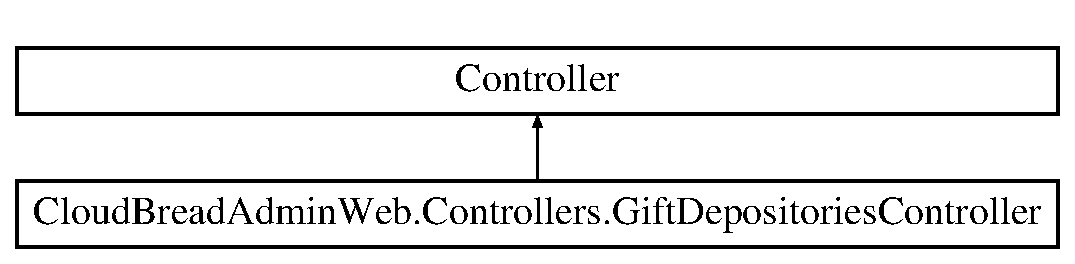
\includegraphics[height=2.000000cm]{a00087}
\end{center}
\end{figure}
\subsection*{Public Member Functions}
\begin{DoxyCompactItemize}
\item 
\hyperlink{a00086}{Gift\+Depositories} {\bfseries Decrypt\+Result} (\hyperlink{a00086}{Gift\+Depositories} item)\hypertarget{a00087_a19a4ed752e8df39fef5d7021427d9dbf}{}\label{a00087_a19a4ed752e8df39fef5d7021427d9dbf}

\item 
\hyperlink{a00086}{Gift\+Depositories} {\bfseries Encrypt\+Result} (\hyperlink{a00086}{Gift\+Depositories} item)\hypertarget{a00087_ad13e8ee4dfa8debf7385d288f1a9c189}{}\label{a00087_ad13e8ee4dfa8debf7385d288f1a9c189}

\item 
bool {\bfseries Check\+Session} ()\hypertarget{a00087_ac83d65a549bd88ca67100b6c279f25c9}{}\label{a00087_ac83d65a549bd88ca67100b6c279f25c9}

\item 
Action\+Result {\bfseries Index} (string search\+String, string Search\+Condition, string current\+Filter, int?page)\hypertarget{a00087_a7b24a6befd1e8d18f61e0db027631729}{}\label{a00087_a7b24a6befd1e8d18f61e0db027631729}

\item 
Action\+Result {\bfseries Details} (string id)\hypertarget{a00087_aa4bbcf592c6168a7ec2f34ad956042bf}{}\label{a00087_aa4bbcf592c6168a7ec2f34ad956042bf}

\item 
Action\+Result {\bfseries Create} ()\hypertarget{a00087_afc99e05312f28141718d0f4660221e4c}{}\label{a00087_afc99e05312f28141718d0f4660221e4c}

\item 
Action\+Result {\bfseries Create} (\mbox{[}Bind(Include=\char`\"{}Gift\+Depository\+ID,Item\+List\+ID,Item\+Count,From\+Member\+ID,To\+Member\+ID,s\+Col1,s\+Col2,s\+Col3,s\+Col4,s\+Col5,s\+Col6,s\+Col7,s\+Col8,s\+Col9,s\+Col10,Sent\+Member\+YN,Hide\+YN,Delete\+YN,Created\+At,Updated\+At,Data\+From\+Region,Data\+From\+Region\+DT\char`\"{})\mbox{]} Gift\+Depositories gift\+Depositories)\hypertarget{a00087_aa35ddc32a96e9cb8dfb4a4b504e1944f}{}\label{a00087_aa35ddc32a96e9cb8dfb4a4b504e1944f}

\item 
Action\+Result {\bfseries Edit} (string id)\hypertarget{a00087_a3f65c373166f83a28de97d61991256eb}{}\label{a00087_a3f65c373166f83a28de97d61991256eb}

\item 
Action\+Result {\bfseries Edit} (\mbox{[}Bind(Include=\char`\"{}Gift\+Depository\+ID,Item\+List\+ID,Item\+Count,From\+Member\+ID,To\+Member\+ID,s\+Col1,s\+Col2,s\+Col3,s\+Col4,s\+Col5,s\+Col6,s\+Col7,s\+Col8,s\+Col9,s\+Col10,Sent\+Member\+YN,Hide\+YN,Delete\+YN,Created\+At,Updated\+At,Data\+From\+Region,Data\+From\+Region\+DT\char`\"{})\mbox{]} Gift\+Depositories gift\+Depositories)\hypertarget{a00087_acf856e4f0533f5e578ad1549b0a297e2}{}\label{a00087_acf856e4f0533f5e578ad1549b0a297e2}

\item 
Action\+Result {\bfseries Delete} (string id)\hypertarget{a00087_a2c4e695e78da9e766126ea5369bc6dfe}{}\label{a00087_a2c4e695e78da9e766126ea5369bc6dfe}

\item 
Action\+Result {\bfseries Delete\+Confirmed} (string id)\hypertarget{a00087_a61fc8612e2273fbd328624e99823ba0d}{}\label{a00087_a61fc8612e2273fbd328624e99823ba0d}

\end{DoxyCompactItemize}
\subsection*{Protected Member Functions}
\begin{DoxyCompactItemize}
\item 
override void {\bfseries Dispose} (bool disposing)\hypertarget{a00087_a1e31b97188c2acb720bc826db28a93e7}{}\label{a00087_a1e31b97188c2acb720bc826db28a93e7}

\end{DoxyCompactItemize}


The documentation for this class was generated from the following file\+:\begin{DoxyCompactItemize}
\item 
C\+:/\+Users/dwkim/\+Documents/\+Git\+Hub/\+Cloud\+Bread/\+Cloud\+Bread\+Admin\+Web/\+Controllers/Gift\+Depositories\+Controller.\+cs\end{DoxyCompactItemize}

\hypertarget{a00088}{}\section{Cloud\+Bread.\+Models.\+Sel\+Gift\+Item\+To\+Me\+Input\+Params Class Reference}
\label{a00088}\index{Cloud\+Bread.\+Models.\+Sel\+Gift\+Item\+To\+Me\+Input\+Params@{Cloud\+Bread.\+Models.\+Sel\+Gift\+Item\+To\+Me\+Input\+Params}}
\subsection*{Properties}
\begin{DoxyCompactItemize}
\item 
string {\bfseries Member\+ID}\hspace{0.3cm}{\ttfamily  \mbox{[}get, set\mbox{]}}\hypertarget{a00088_a26287699ce5150a86c765a1254823a02}{}\label{a00088_a26287699ce5150a86c765a1254823a02}

\item 
string {\bfseries token}\hspace{0.3cm}{\ttfamily  \mbox{[}get, set\mbox{]}}\hypertarget{a00088_aa3997512709afcbb970f5990f3c3ef2b}{}\label{a00088_aa3997512709afcbb970f5990f3c3ef2b}

\end{DoxyCompactItemize}


The documentation for this class was generated from the following file\+:\begin{DoxyCompactItemize}
\item 
C\+:/\+Users/dwkim/\+Documents/\+Git\+Hub/\+Cloud\+Bread/\+Models/Sel\+Gift\+Item\+To\+Me.\+cs\end{DoxyCompactItemize}

\hypertarget{a00089}{}\section{Cloud\+Bread\+Admin\+Web.\+Controllers.\+Home\+Controller Class Reference}
\label{a00089}\index{Cloud\+Bread\+Admin\+Web.\+Controllers.\+Home\+Controller@{Cloud\+Bread\+Admin\+Web.\+Controllers.\+Home\+Controller}}
Inheritance diagram for Cloud\+Bread\+Admin\+Web.\+Controllers.\+Home\+Controller\+:\begin{figure}[H]
\begin{center}
\leavevmode
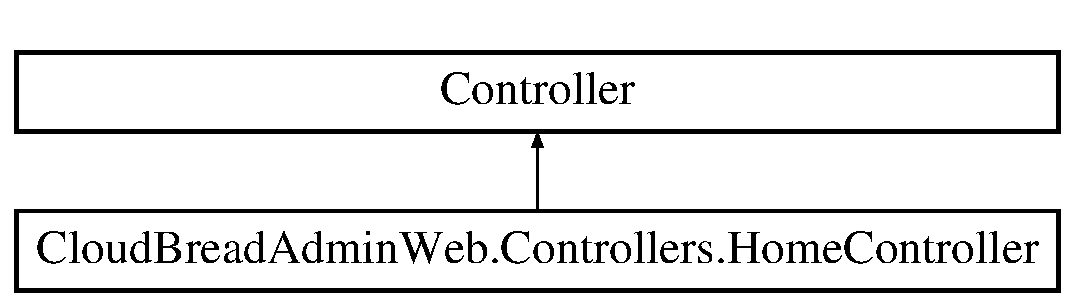
\includegraphics[height=2.000000cm]{a00089}
\end{center}
\end{figure}
\subsection*{Public Member Functions}
\begin{DoxyCompactItemize}
\item 
void {\bfseries Check\+Session} ()\hypertarget{a00089_a4f9e86bf56470506217c3209adc2e59b}{}\label{a00089_a4f9e86bf56470506217c3209adc2e59b}

\item 
Action\+Result {\bfseries Index} ()\hypertarget{a00089_a69cce42d08d6af4d5ff5f9d46a8c0a60}{}\label{a00089_a69cce42d08d6af4d5ff5f9d46a8c0a60}

\item 
Action\+Result {\bfseries Get\+H\+D\+A\+U\+Chart\+Image} ()\hypertarget{a00089_a829e5f205a637734fd6a77fb4f7bd052}{}\label{a00089_a829e5f205a637734fd6a77fb4f7bd052}

\item 
Action\+Result {\bfseries Get\+D\+D\+A\+U\+Chart\+Image} ()\hypertarget{a00089_a111a81c40ef1fe28dca5eaf5ef0cab1f}{}\label{a00089_a111a81c40ef1fe28dca5eaf5ef0cab1f}

\item 
Action\+Result {\bfseries Get\+Cash\+Item\+Chart\+Image} ()\hypertarget{a00089_ae9f2de6d76e9bdd67b618e0a5dbc34a0}{}\label{a00089_ae9f2de6d76e9bdd67b618e0a5dbc34a0}

\end{DoxyCompactItemize}
\subsection*{Public Attributes}
\begin{DoxyCompactItemize}
\item 
\hyperlink{a00065}{Cloud\+Bread\+D\+B\+Admin\+Entities} {\bfseries db} = new \hyperlink{a00065}{Cloud\+Bread\+D\+B\+Admin\+Entities}()\hypertarget{a00089_a348051ae2729879d2c661d5b2376cdab}{}\label{a00089_a348051ae2729879d2c661d5b2376cdab}

\end{DoxyCompactItemize}


The documentation for this class was generated from the following file\+:\begin{DoxyCompactItemize}
\item 
C\+:/\+Users/dwkim/\+Documents/\+Git\+Hub/\+Cloud\+Bread/\+Cloud\+Bread\+Admin\+Web/\+Controllers/Home\+Controller.\+cs\end{DoxyCompactItemize}

\hypertarget{a00090}{}\section{Cloud\+Bread\+Admin\+Web.\+Models.\+Index\+View\+Model Class Reference}
\label{a00090}\index{Cloud\+Bread\+Admin\+Web.\+Models.\+Index\+View\+Model@{Cloud\+Bread\+Admin\+Web.\+Models.\+Index\+View\+Model}}
\subsection*{Properties}
\begin{DoxyCompactItemize}
\item 
bool {\bfseries Has\+Password}\hspace{0.3cm}{\ttfamily  \mbox{[}get, set\mbox{]}}\hypertarget{a00090_a341f3ba7ac181d4a1e839e4053b4a06b}{}\label{a00090_a341f3ba7ac181d4a1e839e4053b4a06b}

\item 
I\+List$<$ User\+Login\+Info $>$ {\bfseries Logins}\hspace{0.3cm}{\ttfamily  \mbox{[}get, set\mbox{]}}\hypertarget{a00090_ae62fc9836800b53b5f9c4e2b858e6257}{}\label{a00090_ae62fc9836800b53b5f9c4e2b858e6257}

\item 
string {\bfseries Phone\+Number}\hspace{0.3cm}{\ttfamily  \mbox{[}get, set\mbox{]}}\hypertarget{a00090_a8f42d419be92c45f1a7952220f34bbe9}{}\label{a00090_a8f42d419be92c45f1a7952220f34bbe9}

\item 
bool {\bfseries Two\+Factor}\hspace{0.3cm}{\ttfamily  \mbox{[}get, set\mbox{]}}\hypertarget{a00090_a5f903d979816303fcafdeff2f530efc8}{}\label{a00090_a5f903d979816303fcafdeff2f530efc8}

\item 
bool {\bfseries Browser\+Remembered}\hspace{0.3cm}{\ttfamily  \mbox{[}get, set\mbox{]}}\hypertarget{a00090_af678dc400ffcf0b9da0500f6bbecd917}{}\label{a00090_af678dc400ffcf0b9da0500f6bbecd917}

\end{DoxyCompactItemize}


The documentation for this class was generated from the following file\+:\begin{DoxyCompactItemize}
\item 
C\+:/\+Users/dwkim/\+Documents/\+Git\+Hub/\+Cloud\+Bread/\+Cloud\+Bread\+Admin\+Web/\+Models/Manage\+View\+Models.\+cs\end{DoxyCompactItemize}

\hypertarget{a00091}{}\section{Cloud\+Bread.\+Models.\+Sel\+Item1\+Model Class Reference}
\label{a00091}\index{Cloud\+Bread.\+Models.\+Sel\+Item1\+Model@{Cloud\+Bread.\+Models.\+Sel\+Item1\+Model}}
\subsection*{Properties}
\begin{DoxyCompactItemize}
\item 
string {\bfseries Item\+List\+ID}\hspace{0.3cm}{\ttfamily  \mbox{[}get, set\mbox{]}}\hypertarget{a00091_a5b9ac7c75055e38add7563beff7088c4}{}\label{a00091_a5b9ac7c75055e38add7563beff7088c4}

\item 
string {\bfseries Item\+Name}\hspace{0.3cm}{\ttfamily  \mbox{[}get, set\mbox{]}}\hypertarget{a00091_aefa03385eeb2061d5bd0b4ace9525972}{}\label{a00091_aefa03385eeb2061d5bd0b4ace9525972}

\item 
string {\bfseries Item\+Description}\hspace{0.3cm}{\ttfamily  \mbox{[}get, set\mbox{]}}\hypertarget{a00091_ac59acb2682eaca0eabd251cef1351320}{}\label{a00091_ac59acb2682eaca0eabd251cef1351320}

\item 
string {\bfseries Item\+Price}\hspace{0.3cm}{\ttfamily  \mbox{[}get, set\mbox{]}}\hypertarget{a00091_a5afe4def8a0c47310aa5fe93b0ba43a7}{}\label{a00091_a5afe4def8a0c47310aa5fe93b0ba43a7}

\item 
string {\bfseries Item\+Sell\+Price}\hspace{0.3cm}{\ttfamily  \mbox{[}get, set\mbox{]}}\hypertarget{a00091_a37f36074466e812ad1fe11b8f5783c77}{}\label{a00091_a37f36074466e812ad1fe11b8f5783c77}

\item 
string {\bfseries Item\+Category1}\hspace{0.3cm}{\ttfamily  \mbox{[}get, set\mbox{]}}\hypertarget{a00091_afcad7716dd3961b23462e701081189cf}{}\label{a00091_afcad7716dd3961b23462e701081189cf}

\item 
string {\bfseries Item\+Category2}\hspace{0.3cm}{\ttfamily  \mbox{[}get, set\mbox{]}}\hypertarget{a00091_a33cd4468986950f423b74afedb2d9b46}{}\label{a00091_a33cd4468986950f423b74afedb2d9b46}

\item 
string {\bfseries Item\+Category3}\hspace{0.3cm}{\ttfamily  \mbox{[}get, set\mbox{]}}\hypertarget{a00091_a56381dfc20e98946a05a4bf2dc212de0}{}\label{a00091_a56381dfc20e98946a05a4bf2dc212de0}

\item 
string {\bfseries s\+Col1}\hspace{0.3cm}{\ttfamily  \mbox{[}get, set\mbox{]}}\hypertarget{a00091_a19d06d74e3fb1dbc4a3997ff694d0505}{}\label{a00091_a19d06d74e3fb1dbc4a3997ff694d0505}

\item 
string {\bfseries s\+Col2}\hspace{0.3cm}{\ttfamily  \mbox{[}get, set\mbox{]}}\hypertarget{a00091_ac8990ce24ff8b92d4028e4f0c234a96d}{}\label{a00091_ac8990ce24ff8b92d4028e4f0c234a96d}

\item 
string {\bfseries s\+Col3}\hspace{0.3cm}{\ttfamily  \mbox{[}get, set\mbox{]}}\hypertarget{a00091_a3c15aeca33dfd3fdc00a0aeff0b3e485}{}\label{a00091_a3c15aeca33dfd3fdc00a0aeff0b3e485}

\item 
string {\bfseries s\+Col4}\hspace{0.3cm}{\ttfamily  \mbox{[}get, set\mbox{]}}\hypertarget{a00091_a8f485eeea35c81b1d046db6524e08468}{}\label{a00091_a8f485eeea35c81b1d046db6524e08468}

\item 
string {\bfseries s\+Col5}\hspace{0.3cm}{\ttfamily  \mbox{[}get, set\mbox{]}}\hypertarget{a00091_a5e90b12200de53cf3f3d695565c83a32}{}\label{a00091_a5e90b12200de53cf3f3d695565c83a32}

\item 
string {\bfseries s\+Col6}\hspace{0.3cm}{\ttfamily  \mbox{[}get, set\mbox{]}}\hypertarget{a00091_a075937aefa2be80f85106e12e7710479}{}\label{a00091_a075937aefa2be80f85106e12e7710479}

\item 
string {\bfseries s\+Col7}\hspace{0.3cm}{\ttfamily  \mbox{[}get, set\mbox{]}}\hypertarget{a00091_afe0a4a204ef6f4818344025d50564853}{}\label{a00091_afe0a4a204ef6f4818344025d50564853}

\item 
string {\bfseries s\+Col8}\hspace{0.3cm}{\ttfamily  \mbox{[}get, set\mbox{]}}\hypertarget{a00091_a38e4142c1e4e0b8208b4c784512f2e9f}{}\label{a00091_a38e4142c1e4e0b8208b4c784512f2e9f}

\item 
string {\bfseries s\+Col9}\hspace{0.3cm}{\ttfamily  \mbox{[}get, set\mbox{]}}\hypertarget{a00091_a9910fa850d912f91c1d738adc433274d}{}\label{a00091_a9910fa850d912f91c1d738adc433274d}

\item 
string {\bfseries s\+Col10}\hspace{0.3cm}{\ttfamily  \mbox{[}get, set\mbox{]}}\hypertarget{a00091_a50a356292c280f177dc988f732f0aae4}{}\label{a00091_a50a356292c280f177dc988f732f0aae4}

\end{DoxyCompactItemize}


The documentation for this class was generated from the following file\+:\begin{DoxyCompactItemize}
\item 
C\+:/\+Users/dwkim/\+Documents/\+Git\+Hub/\+Cloud\+Bread/\+Models/Sel\+Item1.\+cs\end{DoxyCompactItemize}

\hypertarget{a00092}{}\section{Cloud\+Bread.\+Models.\+Sel\+Item\+List\+All\+Input\+Params Class Reference}
\label{a00092}\index{Cloud\+Bread.\+Models.\+Sel\+Item\+List\+All\+Input\+Params@{Cloud\+Bread.\+Models.\+Sel\+Item\+List\+All\+Input\+Params}}
\subsection*{Properties}
\begin{DoxyCompactItemize}
\item 
string {\bfseries Member\+ID}\hspace{0.3cm}{\ttfamily  \mbox{[}get, set\mbox{]}}\hypertarget{a00092_a5a475a536972b1d79537f74d6d8baeea}{}\label{a00092_a5a475a536972b1d79537f74d6d8baeea}

\item 
Int64 {\bfseries Page}\hspace{0.3cm}{\ttfamily  \mbox{[}get, set\mbox{]}}\hypertarget{a00092_a8fef231b4a2f2370e95ca0a7dc7d41fb}{}\label{a00092_a8fef231b4a2f2370e95ca0a7dc7d41fb}

\item 
Int64 {\bfseries Page\+Size}\hspace{0.3cm}{\ttfamily  \mbox{[}get, set\mbox{]}}\hypertarget{a00092_a9280075d26081d3e718f9fc7e54af00d}{}\label{a00092_a9280075d26081d3e718f9fc7e54af00d}

\item 
string {\bfseries token}\hspace{0.3cm}{\ttfamily  \mbox{[}get, set\mbox{]}}\hypertarget{a00092_abc5f713c35457f3a9fa6edabeae87b2b}{}\label{a00092_abc5f713c35457f3a9fa6edabeae87b2b}

\end{DoxyCompactItemize}


The documentation for this class was generated from the following file\+:\begin{DoxyCompactItemize}
\item 
C\+:/\+Users/dwkim/\+Documents/\+Git\+Hub/\+Cloud\+Bread/\+Models/Sel\+Item\+List\+All.\+cs\end{DoxyCompactItemize}

\hypertarget{a00093}{}\section{Cloud\+Bread.\+Models.\+Sel\+Item\+List\+All\+Model Class Reference}
\label{a00093}\index{Cloud\+Bread.\+Models.\+Sel\+Item\+List\+All\+Model@{Cloud\+Bread.\+Models.\+Sel\+Item\+List\+All\+Model}}
\subsection*{Properties}
\begin{DoxyCompactItemize}
\item 
string {\bfseries R\+O\+W\+N\+UM}\hspace{0.3cm}{\ttfamily  \mbox{[}get, set\mbox{]}}\hypertarget{a00093_a8ffa368d845015e056d5dbf1afceabe1}{}\label{a00093_a8ffa368d845015e056d5dbf1afceabe1}

\item 
string {\bfseries Item\+List\+ID}\hspace{0.3cm}{\ttfamily  \mbox{[}get, set\mbox{]}}\hypertarget{a00093_a3f726cf03f37251dee2d3315f3206e5d}{}\label{a00093_a3f726cf03f37251dee2d3315f3206e5d}

\item 
string {\bfseries Item\+Name}\hspace{0.3cm}{\ttfamily  \mbox{[}get, set\mbox{]}}\hypertarget{a00093_a2c6ae509d1412994646a85f5c854d518}{}\label{a00093_a2c6ae509d1412994646a85f5c854d518}

\item 
string {\bfseries Item\+Description}\hspace{0.3cm}{\ttfamily  \mbox{[}get, set\mbox{]}}\hypertarget{a00093_aa95c3815d64954a801c511d76b33f40e}{}\label{a00093_aa95c3815d64954a801c511d76b33f40e}

\item 
string {\bfseries Item\+Price}\hspace{0.3cm}{\ttfamily  \mbox{[}get, set\mbox{]}}\hypertarget{a00093_af1f84607f3fc7a2ae3fc67d398257ba9}{}\label{a00093_af1f84607f3fc7a2ae3fc67d398257ba9}

\item 
string {\bfseries Item\+Sell\+Price}\hspace{0.3cm}{\ttfamily  \mbox{[}get, set\mbox{]}}\hypertarget{a00093_a870420c0dce3559cd4ce664270c83780}{}\label{a00093_a870420c0dce3559cd4ce664270c83780}

\item 
string {\bfseries Item\+Category1}\hspace{0.3cm}{\ttfamily  \mbox{[}get, set\mbox{]}}\hypertarget{a00093_a200d8b80c6849d61d3aaa46306fbe786}{}\label{a00093_a200d8b80c6849d61d3aaa46306fbe786}

\item 
string {\bfseries Item\+Category2}\hspace{0.3cm}{\ttfamily  \mbox{[}get, set\mbox{]}}\hypertarget{a00093_a793c7623b114144d2e815db1f7ea09a8}{}\label{a00093_a793c7623b114144d2e815db1f7ea09a8}

\item 
string {\bfseries Item\+Category3}\hspace{0.3cm}{\ttfamily  \mbox{[}get, set\mbox{]}}\hypertarget{a00093_a3703e9ec2a355fd495c2aa894c08ca57}{}\label{a00093_a3703e9ec2a355fd495c2aa894c08ca57}

\item 
string {\bfseries s\+Col1}\hspace{0.3cm}{\ttfamily  \mbox{[}get, set\mbox{]}}\hypertarget{a00093_adabea4b28a9b4ea633621fb2d2010ab7}{}\label{a00093_adabea4b28a9b4ea633621fb2d2010ab7}

\item 
string {\bfseries s\+Col2}\hspace{0.3cm}{\ttfamily  \mbox{[}get, set\mbox{]}}\hypertarget{a00093_aff318bc13fee48ae9e6b95e03be8c5ec}{}\label{a00093_aff318bc13fee48ae9e6b95e03be8c5ec}

\item 
string {\bfseries s\+Col3}\hspace{0.3cm}{\ttfamily  \mbox{[}get, set\mbox{]}}\hypertarget{a00093_a75cecc7bd4f6e4ea36792b44120cae77}{}\label{a00093_a75cecc7bd4f6e4ea36792b44120cae77}

\item 
string {\bfseries s\+Col4}\hspace{0.3cm}{\ttfamily  \mbox{[}get, set\mbox{]}}\hypertarget{a00093_afe8e062490f6ec7932e6db4cfffd8ac4}{}\label{a00093_afe8e062490f6ec7932e6db4cfffd8ac4}

\item 
string {\bfseries s\+Col5}\hspace{0.3cm}{\ttfamily  \mbox{[}get, set\mbox{]}}\hypertarget{a00093_ae1d08b7942ac1362e19d2b1d45b36db5}{}\label{a00093_ae1d08b7942ac1362e19d2b1d45b36db5}

\item 
string {\bfseries s\+Col6}\hspace{0.3cm}{\ttfamily  \mbox{[}get, set\mbox{]}}\hypertarget{a00093_a50582f29f8dc67ecae7000d825495950}{}\label{a00093_a50582f29f8dc67ecae7000d825495950}

\item 
string {\bfseries s\+Col7}\hspace{0.3cm}{\ttfamily  \mbox{[}get, set\mbox{]}}\hypertarget{a00093_a86297f899e8efdc9fd731dac564c55c7}{}\label{a00093_a86297f899e8efdc9fd731dac564c55c7}

\item 
string {\bfseries s\+Col8}\hspace{0.3cm}{\ttfamily  \mbox{[}get, set\mbox{]}}\hypertarget{a00093_a3491fefa0103ab19fa4474aee9974b3c}{}\label{a00093_a3491fefa0103ab19fa4474aee9974b3c}

\item 
string {\bfseries s\+Col9}\hspace{0.3cm}{\ttfamily  \mbox{[}get, set\mbox{]}}\hypertarget{a00093_a5479281dab4d64c932ef28fc62a9d53f}{}\label{a00093_a5479281dab4d64c932ef28fc62a9d53f}

\item 
string {\bfseries s\+Col10}\hspace{0.3cm}{\ttfamily  \mbox{[}get, set\mbox{]}}\hypertarget{a00093_a1e85d83fcdc0ca357f6e90dfce758df9}{}\label{a00093_a1e85d83fcdc0ca357f6e90dfce758df9}

\end{DoxyCompactItemize}


The documentation for this class was generated from the following file\+:\begin{DoxyCompactItemize}
\item 
C\+:/\+Users/dwkim/\+Documents/\+Git\+Hub/\+Cloud\+Bread/\+Models/Sel\+Item\+List\+All.\+cs\end{DoxyCompactItemize}

\hypertarget{a00094}{}\section{Cloud\+Bread.\+Controllers.\+C\+B\+Com\+Udt\+Item\+List1\+Controller.\+Input\+Params Class Reference}
\label{a00094}\index{Cloud\+Bread.\+Controllers.\+C\+B\+Com\+Udt\+Item\+List1\+Controller.\+Input\+Params@{Cloud\+Bread.\+Controllers.\+C\+B\+Com\+Udt\+Item\+List1\+Controller.\+Input\+Params}}
\subsection*{Properties}
\begin{DoxyCompactItemize}
\item 
string {\bfseries Member\+ID}\hspace{0.3cm}{\ttfamily  \mbox{[}get, set\mbox{]}}\hypertarget{a00094_aefe5c8c92140de3b72cc5033e2559b6c}{}\label{a00094_aefe5c8c92140de3b72cc5033e2559b6c}

\item 
string {\bfseries Item\+List\+ID}\hspace{0.3cm}{\ttfamily  \mbox{[}get, set\mbox{]}}\hypertarget{a00094_a740d4e0657cb37f12bdacc6660d74bb5}{}\label{a00094_a740d4e0657cb37f12bdacc6660d74bb5}

\item 
string {\bfseries Item\+Name}\hspace{0.3cm}{\ttfamily  \mbox{[}get, set\mbox{]}}\hypertarget{a00094_abd815de9bebbcc10271c255582122f39}{}\label{a00094_abd815de9bebbcc10271c255582122f39}

\item 
string {\bfseries Item\+Description}\hspace{0.3cm}{\ttfamily  \mbox{[}get, set\mbox{]}}\hypertarget{a00094_aa656ee374dfa31edf29427c5cf130001}{}\label{a00094_aa656ee374dfa31edf29427c5cf130001}

\item 
string {\bfseries Item\+Price}\hspace{0.3cm}{\ttfamily  \mbox{[}get, set\mbox{]}}\hypertarget{a00094_a8cd89b7b327e7645a9e8af4af477a5e0}{}\label{a00094_a8cd89b7b327e7645a9e8af4af477a5e0}

\item 
string {\bfseries Item\+Sell\+Price}\hspace{0.3cm}{\ttfamily  \mbox{[}get, set\mbox{]}}\hypertarget{a00094_ad2c6aa992e02e7807d3b203b51990e44}{}\label{a00094_ad2c6aa992e02e7807d3b203b51990e44}

\item 
string {\bfseries Item\+Category1}\hspace{0.3cm}{\ttfamily  \mbox{[}get, set\mbox{]}}\hypertarget{a00094_a029fc009a1436681d324408ef2ea4917}{}\label{a00094_a029fc009a1436681d324408ef2ea4917}

\item 
string {\bfseries Item\+Category2}\hspace{0.3cm}{\ttfamily  \mbox{[}get, set\mbox{]}}\hypertarget{a00094_a060c5b22057643198ecd9722c0736447}{}\label{a00094_a060c5b22057643198ecd9722c0736447}

\item 
string {\bfseries Item\+Category3}\hspace{0.3cm}{\ttfamily  \mbox{[}get, set\mbox{]}}\hypertarget{a00094_ab7ae2ade4146e00cba4848775092dc3b}{}\label{a00094_ab7ae2ade4146e00cba4848775092dc3b}

\item 
string {\bfseries s\+Col1}\hspace{0.3cm}{\ttfamily  \mbox{[}get, set\mbox{]}}\hypertarget{a00094_a2afcc1c3587462f9c15e6d51d8d5fdac}{}\label{a00094_a2afcc1c3587462f9c15e6d51d8d5fdac}

\item 
string {\bfseries s\+Col2}\hspace{0.3cm}{\ttfamily  \mbox{[}get, set\mbox{]}}\hypertarget{a00094_ad5545c6d3a172a9206edf6b025e627fe}{}\label{a00094_ad5545c6d3a172a9206edf6b025e627fe}

\item 
string {\bfseries s\+Col3}\hspace{0.3cm}{\ttfamily  \mbox{[}get, set\mbox{]}}\hypertarget{a00094_a8b09ab88118992d3f6a58fef26d64706}{}\label{a00094_a8b09ab88118992d3f6a58fef26d64706}

\item 
string {\bfseries s\+Col4}\hspace{0.3cm}{\ttfamily  \mbox{[}get, set\mbox{]}}\hypertarget{a00094_a4b3e3d1e82931ddc6448acb20fd7f80d}{}\label{a00094_a4b3e3d1e82931ddc6448acb20fd7f80d}

\item 
string {\bfseries s\+Col5}\hspace{0.3cm}{\ttfamily  \mbox{[}get, set\mbox{]}}\hypertarget{a00094_a4bc16a0d54a5a8049113757c9cc61128}{}\label{a00094_a4bc16a0d54a5a8049113757c9cc61128}

\item 
string {\bfseries s\+Col6}\hspace{0.3cm}{\ttfamily  \mbox{[}get, set\mbox{]}}\hypertarget{a00094_a5ef85fef0f24c884b67508431affbb6c}{}\label{a00094_a5ef85fef0f24c884b67508431affbb6c}

\item 
string {\bfseries s\+Col7}\hspace{0.3cm}{\ttfamily  \mbox{[}get, set\mbox{]}}\hypertarget{a00094_a76486b94a72b7d1e02609a2dbcbc4740}{}\label{a00094_a76486b94a72b7d1e02609a2dbcbc4740}

\item 
string {\bfseries s\+Col8}\hspace{0.3cm}{\ttfamily  \mbox{[}get, set\mbox{]}}\hypertarget{a00094_a81367fc2cfa35393431a666c0eff8929}{}\label{a00094_a81367fc2cfa35393431a666c0eff8929}

\item 
string {\bfseries s\+Col9}\hspace{0.3cm}{\ttfamily  \mbox{[}get, set\mbox{]}}\hypertarget{a00094_aa5aaa83b201c704a476f95744d9e3cda}{}\label{a00094_aa5aaa83b201c704a476f95744d9e3cda}

\item 
string {\bfseries s\+Col10}\hspace{0.3cm}{\ttfamily  \mbox{[}get, set\mbox{]}}\hypertarget{a00094_aae0c9304e695b4a77f16e29cfc938568}{}\label{a00094_aae0c9304e695b4a77f16e29cfc938568}

\end{DoxyCompactItemize}


The documentation for this class was generated from the following file\+:\begin{DoxyCompactItemize}
\item 
C\+:/\+Users/dwkim/\+Documents/\+Git\+Hub/\+Cloud\+Bread/\+Cloud\+Bread/\+Controllers/\hyperlink{a00208}{C\+B\+Com\+Udt\+Item\+List1\+Controller.\+cs}\end{DoxyCompactItemize}

\hypertarget{a00095}{}\section{Cloud\+Bread.\+Controllers.\+C\+B\+Com\+Sel\+Member\+Controller.\+Input\+Params Class Reference}
\label{a00095}\index{Cloud\+Bread.\+Controllers.\+C\+B\+Com\+Sel\+Member\+Controller.\+Input\+Params@{Cloud\+Bread.\+Controllers.\+C\+B\+Com\+Sel\+Member\+Controller.\+Input\+Params}}
\subsection*{Public Attributes}
\begin{DoxyCompactItemize}
\item 
string {\bfseries member\+ID}\hypertarget{a00095_ad75a94e40a6bda7b1177c7a30560a79e}{}\label{a00095_ad75a94e40a6bda7b1177c7a30560a79e}

\end{DoxyCompactItemize}


The documentation for this class was generated from the following file\+:\begin{DoxyCompactItemize}
\item 
C\+:/\+Users/dwkim/\+Documents/\+Git\+Hub/\+Cloud\+Bread/\+Cloud\+Bread/\+Controllers/\hyperlink{a00202}{C\+B\+Com\+Sel\+Member\+Controller.\+cs}\end{DoxyCompactItemize}

\hypertarget{a00096}{}\section{Cloud\+Bread.\+Controllers.\+C\+B\+Sel\+Member\+Game\+Info\+Stages\+Controller.\+Input\+Params Class Reference}
\label{a00096}\index{Cloud\+Bread.\+Controllers.\+C\+B\+Sel\+Member\+Game\+Info\+Stages\+Controller.\+Input\+Params@{Cloud\+Bread.\+Controllers.\+C\+B\+Sel\+Member\+Game\+Info\+Stages\+Controller.\+Input\+Params}}
\subsection*{Public Attributes}
\begin{DoxyCompactItemize}
\item 
string {\bfseries member\+ID}\hypertarget{a00096_a591a11a0c69188fdf44a4aaf9c4d7562}{}\label{a00096_a591a11a0c69188fdf44a4aaf9c4d7562}

\end{DoxyCompactItemize}


The documentation for this class was generated from the following file\+:\begin{DoxyCompactItemize}
\item 
C\+:/\+Users/dwkim/\+Documents/\+Git\+Hub/\+Cloud\+Bread/\+Cloud\+Bread/\+Controllers/\hyperlink{a00223}{C\+B\+Sel\+Member\+Game\+Info\+Stages\+Controller.\+cs}\end{DoxyCompactItemize}

\hypertarget{a00097}{}\section{Cloud\+Bread.\+Models.\+Sel\+Login\+Info\+Model Class Reference}
\label{a00097}\index{Cloud\+Bread.\+Models.\+Sel\+Login\+Info\+Model@{Cloud\+Bread.\+Models.\+Sel\+Login\+Info\+Model}}
\subsection*{Properties}
\begin{DoxyCompactItemize}
\item 
string {\bfseries Member\+ID}\hspace{0.3cm}{\ttfamily  \mbox{[}get, set\mbox{]}}\hypertarget{a00097_a0553755eb11ace1f2a821085993cc46c}{}\label{a00097_a0553755eb11ace1f2a821085993cc46c}

\item 
string {\bfseries Member\+P\+WD}\hspace{0.3cm}{\ttfamily  \mbox{[}get, set\mbox{]}}\hypertarget{a00097_a9b2e01bdd29277ba57efe99308ac4bfc}{}\label{a00097_a9b2e01bdd29277ba57efe99308ac4bfc}

\item 
string {\bfseries Email\+Address}\hspace{0.3cm}{\ttfamily  \mbox{[}get, set\mbox{]}}\hypertarget{a00097_ae7ff33c5a0c86b2d5f2a3040e00ed8df}{}\label{a00097_ae7ff33c5a0c86b2d5f2a3040e00ed8df}

\item 
string {\bfseries Email\+Confirmed\+YN}\hspace{0.3cm}{\ttfamily  \mbox{[}get, set\mbox{]}}\hypertarget{a00097_a0aeb823b334a90226a99a0332b27b852}{}\label{a00097_a0aeb823b334a90226a99a0332b27b852}

\item 
string {\bfseries Phone\+Number1}\hspace{0.3cm}{\ttfamily  \mbox{[}get, set\mbox{]}}\hypertarget{a00097_a7a46683c70a091c34ee4309ebb0dbceb}{}\label{a00097_a7a46683c70a091c34ee4309ebb0dbceb}

\item 
string {\bfseries Phone\+Number2}\hspace{0.3cm}{\ttfamily  \mbox{[}get, set\mbox{]}}\hypertarget{a00097_ad570a8e9b4e834023a587457bdf815f5}{}\label{a00097_ad570a8e9b4e834023a587457bdf815f5}

\item 
string {\bfseries P\+I\+Number}\hspace{0.3cm}{\ttfamily  \mbox{[}get, set\mbox{]}}\hypertarget{a00097_a779a299665336e1cb431e0745dceeafc}{}\label{a00097_a779a299665336e1cb431e0745dceeafc}

\item 
string {\bfseries Name1}\hspace{0.3cm}{\ttfamily  \mbox{[}get, set\mbox{]}}\hypertarget{a00097_a2470f2dff10ca643081eafcf12bee030}{}\label{a00097_a2470f2dff10ca643081eafcf12bee030}

\item 
string {\bfseries Name2}\hspace{0.3cm}{\ttfamily  \mbox{[}get, set\mbox{]}}\hypertarget{a00097_a1208d7c34d224bf88113d3717a20741a}{}\label{a00097_a1208d7c34d224bf88113d3717a20741a}

\item 
string {\bfseries Name3}\hspace{0.3cm}{\ttfamily  \mbox{[}get, set\mbox{]}}\hypertarget{a00097_af2cc8a1fa285db7db9c0a95effbb66dd}{}\label{a00097_af2cc8a1fa285db7db9c0a95effbb66dd}

\item 
string {\bfseries D\+OB}\hspace{0.3cm}{\ttfamily  \mbox{[}get, set\mbox{]}}\hypertarget{a00097_a1830c867262099c1fa9383a67a82c858}{}\label{a00097_a1830c867262099c1fa9383a67a82c858}

\item 
string {\bfseries Recommender\+ID}\hspace{0.3cm}{\ttfamily  \mbox{[}get, set\mbox{]}}\hypertarget{a00097_ae199167ef43c905a8c5a7260e4d26faa}{}\label{a00097_ae199167ef43c905a8c5a7260e4d26faa}

\item 
string {\bfseries Member\+Group}\hspace{0.3cm}{\ttfamily  \mbox{[}get, set\mbox{]}}\hypertarget{a00097_aefeb389eb5fb1c977b30a367ef518097}{}\label{a00097_aefeb389eb5fb1c977b30a367ef518097}

\item 
string {\bfseries Last\+Device\+ID}\hspace{0.3cm}{\ttfamily  \mbox{[}get, set\mbox{]}}\hypertarget{a00097_abd5bd06fa377d62c22549d84db122869}{}\label{a00097_abd5bd06fa377d62c22549d84db122869}

\item 
string {\bfseries Last\+I\+Paddress}\hspace{0.3cm}{\ttfamily  \mbox{[}get, set\mbox{]}}\hypertarget{a00097_a7ff78ddcda577fabf22df2202aa9df0d}{}\label{a00097_a7ff78ddcda577fabf22df2202aa9df0d}

\item 
string {\bfseries Last\+Login\+DT}\hspace{0.3cm}{\ttfamily  \mbox{[}get, set\mbox{]}}\hypertarget{a00097_ab272be3f6451c094f08df150aa08047f}{}\label{a00097_ab272be3f6451c094f08df150aa08047f}

\item 
string {\bfseries Last\+Logout\+DT}\hspace{0.3cm}{\ttfamily  \mbox{[}get, set\mbox{]}}\hypertarget{a00097_a6a48ef1a73e42a6c3ff6e2c0d28650d0}{}\label{a00097_a6a48ef1a73e42a6c3ff6e2c0d28650d0}

\item 
string {\bfseries Last\+M\+A\+C\+Address}\hspace{0.3cm}{\ttfamily  \mbox{[}get, set\mbox{]}}\hypertarget{a00097_afebaef735a72cc24883412c9c58fc17e}{}\label{a00097_afebaef735a72cc24883412c9c58fc17e}

\item 
string {\bfseries Account\+Block\+YN}\hspace{0.3cm}{\ttfamily  \mbox{[}get, set\mbox{]}}\hypertarget{a00097_abb0b9438beea58398f28b00370cd86c8}{}\label{a00097_abb0b9438beea58398f28b00370cd86c8}

\item 
string {\bfseries Account\+Block\+End\+DT}\hspace{0.3cm}{\ttfamily  \mbox{[}get, set\mbox{]}}\hypertarget{a00097_a1e7ab9c565cc6c2f260f1921cd91df39}{}\label{a00097_a1e7ab9c565cc6c2f260f1921cd91df39}

\item 
string {\bfseries Anonymous\+YN}\hspace{0.3cm}{\ttfamily  \mbox{[}get, set\mbox{]}}\hypertarget{a00097_a473253b0654620d2c895028026d8dd92}{}\label{a00097_a473253b0654620d2c895028026d8dd92}

\item 
string {\bfseries \+\_\+3rd\+Auth\+Provider}\hspace{0.3cm}{\ttfamily  \mbox{[}get, set\mbox{]}}\hypertarget{a00097_a34170914fa82a66b0f7df78563a240f9}{}\label{a00097_a34170914fa82a66b0f7df78563a240f9}

\item 
string {\bfseries \+\_\+3rd\+Auth\+ID}\hspace{0.3cm}{\ttfamily  \mbox{[}get, set\mbox{]}}\hypertarget{a00097_a68697de4cc14f32ebaa26c6ef6cc630b}{}\label{a00097_a68697de4cc14f32ebaa26c6ef6cc630b}

\item 
string {\bfseries \+\_\+3rd\+Auth\+Param}\hspace{0.3cm}{\ttfamily  \mbox{[}get, set\mbox{]}}\hypertarget{a00097_aa6e9e84a202968f04dd68261a1686b33}{}\label{a00097_aa6e9e84a202968f04dd68261a1686b33}

\item 
string {\bfseries Push\+Notification\+ID}\hspace{0.3cm}{\ttfamily  \mbox{[}get, set\mbox{]}}\hypertarget{a00097_aa8a9bf435f5c4046452141bd2ffc8bc1}{}\label{a00097_aa8a9bf435f5c4046452141bd2ffc8bc1}

\item 
string {\bfseries Push\+Notification\+Provider}\hspace{0.3cm}{\ttfamily  \mbox{[}get, set\mbox{]}}\hypertarget{a00097_ac75f89fd5b60bca0494679382c77cad7}{}\label{a00097_ac75f89fd5b60bca0494679382c77cad7}

\item 
string {\bfseries Push\+Notification\+Group}\hspace{0.3cm}{\ttfamily  \mbox{[}get, set\mbox{]}}\hypertarget{a00097_a7497128050cfc6a52ac258bb843983e0}{}\label{a00097_a7497128050cfc6a52ac258bb843983e0}

\item 
string {\bfseries s\+Col1}\hspace{0.3cm}{\ttfamily  \mbox{[}get, set\mbox{]}}\hypertarget{a00097_a3b373bca54eb0d585cebfaf3f67499f4}{}\label{a00097_a3b373bca54eb0d585cebfaf3f67499f4}

\item 
string {\bfseries s\+Col2}\hspace{0.3cm}{\ttfamily  \mbox{[}get, set\mbox{]}}\hypertarget{a00097_a74bdb45ec35cc76f56710262e87ad110}{}\label{a00097_a74bdb45ec35cc76f56710262e87ad110}

\item 
string {\bfseries s\+Col3}\hspace{0.3cm}{\ttfamily  \mbox{[}get, set\mbox{]}}\hypertarget{a00097_a058e76ad8005e80736d67f5542baf6d4}{}\label{a00097_a058e76ad8005e80736d67f5542baf6d4}

\item 
string {\bfseries s\+Col4}\hspace{0.3cm}{\ttfamily  \mbox{[}get, set\mbox{]}}\hypertarget{a00097_aa798d7ecd792ca2a53a7506d1acccbb1}{}\label{a00097_aa798d7ecd792ca2a53a7506d1acccbb1}

\item 
string {\bfseries s\+Col5}\hspace{0.3cm}{\ttfamily  \mbox{[}get, set\mbox{]}}\hypertarget{a00097_aed4ddb5fc66c2c4ee881271bf76086b2}{}\label{a00097_aed4ddb5fc66c2c4ee881271bf76086b2}

\item 
string {\bfseries s\+Col6}\hspace{0.3cm}{\ttfamily  \mbox{[}get, set\mbox{]}}\hypertarget{a00097_a346e4f86a18d81894e3feff9789789b1}{}\label{a00097_a346e4f86a18d81894e3feff9789789b1}

\item 
string {\bfseries s\+Col7}\hspace{0.3cm}{\ttfamily  \mbox{[}get, set\mbox{]}}\hypertarget{a00097_a8213f2f59e1cf245bae229e64a5377ca}{}\label{a00097_a8213f2f59e1cf245bae229e64a5377ca}

\item 
string {\bfseries s\+Col8}\hspace{0.3cm}{\ttfamily  \mbox{[}get, set\mbox{]}}\hypertarget{a00097_ac8650d2ccf32ca68058ec7a926d0c1dd}{}\label{a00097_ac8650d2ccf32ca68058ec7a926d0c1dd}

\item 
string {\bfseries s\+Col9}\hspace{0.3cm}{\ttfamily  \mbox{[}get, set\mbox{]}}\hypertarget{a00097_a5669959338ff9bb98b4286a7d192eb1c}{}\label{a00097_a5669959338ff9bb98b4286a7d192eb1c}

\item 
string {\bfseries s\+Col10}\hspace{0.3cm}{\ttfamily  \mbox{[}get, set\mbox{]}}\hypertarget{a00097_afb1ea28aca8ba7a357e3c95a6436dd14}{}\label{a00097_afb1ea28aca8ba7a357e3c95a6436dd14}

\end{DoxyCompactItemize}


The documentation for this class was generated from the following file\+:\begin{DoxyCompactItemize}
\item 
C\+:/\+Users/dwkim/\+Documents/\+Git\+Hub/\+Cloud\+Bread/\+Models/Sel\+Login\+Info.\+cs\end{DoxyCompactItemize}

\hypertarget{a00098}{}\section{Cloud\+Bread.\+Controllers.\+C\+B\+Sel\+Member\+Items\+Controller.\+Input\+Params Class Reference}
\label{a00098}\index{Cloud\+Bread.\+Controllers.\+C\+B\+Sel\+Member\+Items\+Controller.\+Input\+Params@{Cloud\+Bread.\+Controllers.\+C\+B\+Sel\+Member\+Items\+Controller.\+Input\+Params}}
\subsection*{Public Attributes}
\begin{DoxyCompactItemize}
\item 
string {\bfseries Member\+ID}\hypertarget{a00098_a38b1ef707609faaa2ddc2fcdf3311ef8}{}\label{a00098_a38b1ef707609faaa2ddc2fcdf3311ef8}

\item 
Int64 {\bfseries Page}\hypertarget{a00098_a94ad166a7dc3fdd11ae7272f7536df3b}{}\label{a00098_a94ad166a7dc3fdd11ae7272f7536df3b}

\item 
Int64 {\bfseries Page\+Size}\hypertarget{a00098_a74aa66e4419f55454037db8a5d14b046}{}\label{a00098_a74aa66e4419f55454037db8a5d14b046}

\end{DoxyCompactItemize}


The documentation for this class was generated from the following file\+:\begin{DoxyCompactItemize}
\item 
C\+:/\+Users/dwkim/\+Documents/\+Git\+Hub/\+Cloud\+Bread/\+Cloud\+Bread/\+Controllers/\hyperlink{a00224}{C\+B\+Sel\+Member\+Items\+Controller.\+cs}\end{DoxyCompactItemize}

\hypertarget{a00099}{}\section{Cloud\+Bread.\+Controllers.\+C\+B\+Com\+Udt\+Member\+Game\+Infoes\+Controller.\+Input\+Params Class Reference}
\label{a00099}\index{Cloud\+Bread.\+Controllers.\+C\+B\+Com\+Udt\+Member\+Game\+Infoes\+Controller.\+Input\+Params@{Cloud\+Bread.\+Controllers.\+C\+B\+Com\+Udt\+Member\+Game\+Infoes\+Controller.\+Input\+Params}}
\subsection*{Properties}
\begin{DoxyCompactItemize}
\item 
string {\bfseries Member\+ID}\hspace{0.3cm}{\ttfamily  \mbox{[}get, set\mbox{]}}\hypertarget{a00099_a9a70f01709d151bfbc05a30d744bffc4}{}\label{a00099_a9a70f01709d151bfbc05a30d744bffc4}

\item 
string {\bfseries Level}\hspace{0.3cm}{\ttfamily  \mbox{[}get, set\mbox{]}}\hypertarget{a00099_ab7493b51b92fa1174b7cfb7d368e0e10}{}\label{a00099_ab7493b51b92fa1174b7cfb7d368e0e10}

\item 
string {\bfseries Exps}\hspace{0.3cm}{\ttfamily  \mbox{[}get, set\mbox{]}}\hypertarget{a00099_a138ecd4302575c63e690afe3fc0ded97}{}\label{a00099_a138ecd4302575c63e690afe3fc0ded97}

\item 
string {\bfseries Points}\hspace{0.3cm}{\ttfamily  \mbox{[}get, set\mbox{]}}\hypertarget{a00099_aab79d983babaa8c4c3cf75913752d7c2}{}\label{a00099_aab79d983babaa8c4c3cf75913752d7c2}

\item 
string {\bfseries User\+S\+T\+A\+T1}\hspace{0.3cm}{\ttfamily  \mbox{[}get, set\mbox{]}}\hypertarget{a00099_a45541763be518598705e7a09a29834cc}{}\label{a00099_a45541763be518598705e7a09a29834cc}

\item 
string {\bfseries User\+S\+T\+A\+T2}\hspace{0.3cm}{\ttfamily  \mbox{[}get, set\mbox{]}}\hypertarget{a00099_a232d52b29f135a153c630f4b92228c3b}{}\label{a00099_a232d52b29f135a153c630f4b92228c3b}

\item 
string {\bfseries User\+S\+T\+A\+T3}\hspace{0.3cm}{\ttfamily  \mbox{[}get, set\mbox{]}}\hypertarget{a00099_a49da70387b0608fa14918bc0973f4bd9}{}\label{a00099_a49da70387b0608fa14918bc0973f4bd9}

\item 
string {\bfseries User\+S\+T\+A\+T4}\hspace{0.3cm}{\ttfamily  \mbox{[}get, set\mbox{]}}\hypertarget{a00099_affb95f3784529f83292e1d703c84b237}{}\label{a00099_affb95f3784529f83292e1d703c84b237}

\item 
string {\bfseries User\+S\+T\+A\+T5}\hspace{0.3cm}{\ttfamily  \mbox{[}get, set\mbox{]}}\hypertarget{a00099_a03ae02f3cde1e98ec80ad73566ef9630}{}\label{a00099_a03ae02f3cde1e98ec80ad73566ef9630}

\item 
string {\bfseries User\+S\+T\+A\+T6}\hspace{0.3cm}{\ttfamily  \mbox{[}get, set\mbox{]}}\hypertarget{a00099_a49343a5abbbc4c7c59b31fcbc36b3ef8}{}\label{a00099_a49343a5abbbc4c7c59b31fcbc36b3ef8}

\item 
string {\bfseries User\+S\+T\+A\+T7}\hspace{0.3cm}{\ttfamily  \mbox{[}get, set\mbox{]}}\hypertarget{a00099_aaace747e00c286569e15393a07274f06}{}\label{a00099_aaace747e00c286569e15393a07274f06}

\item 
string {\bfseries User\+S\+T\+A\+T8}\hspace{0.3cm}{\ttfamily  \mbox{[}get, set\mbox{]}}\hypertarget{a00099_ad39a6e1c1e22404451b10e2f685c60cf}{}\label{a00099_ad39a6e1c1e22404451b10e2f685c60cf}

\item 
string {\bfseries User\+S\+T\+A\+T9}\hspace{0.3cm}{\ttfamily  \mbox{[}get, set\mbox{]}}\hypertarget{a00099_ab0b88ac17c1d796cbe368a512d0469a2}{}\label{a00099_ab0b88ac17c1d796cbe368a512d0469a2}

\item 
string {\bfseries User\+S\+T\+A\+T10}\hspace{0.3cm}{\ttfamily  \mbox{[}get, set\mbox{]}}\hypertarget{a00099_a91343f948a5194c3afa667c9c9b52168}{}\label{a00099_a91343f948a5194c3afa667c9c9b52168}

\item 
string {\bfseries s\+Col1}\hspace{0.3cm}{\ttfamily  \mbox{[}get, set\mbox{]}}\hypertarget{a00099_a8a70cda57708568d849c5cf61934e7d2}{}\label{a00099_a8a70cda57708568d849c5cf61934e7d2}

\item 
string {\bfseries s\+Col2}\hspace{0.3cm}{\ttfamily  \mbox{[}get, set\mbox{]}}\hypertarget{a00099_a197475cb1ebad270b3a711cb00908451}{}\label{a00099_a197475cb1ebad270b3a711cb00908451}

\item 
string {\bfseries s\+Col3}\hspace{0.3cm}{\ttfamily  \mbox{[}get, set\mbox{]}}\hypertarget{a00099_aef1f0fdbf5a3c15cab1c53f3583d397d}{}\label{a00099_aef1f0fdbf5a3c15cab1c53f3583d397d}

\item 
string {\bfseries s\+Col4}\hspace{0.3cm}{\ttfamily  \mbox{[}get, set\mbox{]}}\hypertarget{a00099_aacd8e645ec251acc7431ec5bbfa5b571}{}\label{a00099_aacd8e645ec251acc7431ec5bbfa5b571}

\item 
string {\bfseries s\+Col5}\hspace{0.3cm}{\ttfamily  \mbox{[}get, set\mbox{]}}\hypertarget{a00099_aedb88258b20967b39be49214b5a7c72d}{}\label{a00099_aedb88258b20967b39be49214b5a7c72d}

\item 
string {\bfseries s\+Col6}\hspace{0.3cm}{\ttfamily  \mbox{[}get, set\mbox{]}}\hypertarget{a00099_a3a461bd6e04837892c694c52a3389ec0}{}\label{a00099_a3a461bd6e04837892c694c52a3389ec0}

\item 
string {\bfseries s\+Col7}\hspace{0.3cm}{\ttfamily  \mbox{[}get, set\mbox{]}}\hypertarget{a00099_a3f316515b99b1fede79a3ebba3419080}{}\label{a00099_a3f316515b99b1fede79a3ebba3419080}

\item 
string {\bfseries s\+Col8}\hspace{0.3cm}{\ttfamily  \mbox{[}get, set\mbox{]}}\hypertarget{a00099_a18dd83fc8f7d231c98486829abe9e67e}{}\label{a00099_a18dd83fc8f7d231c98486829abe9e67e}

\item 
string {\bfseries s\+Col9}\hspace{0.3cm}{\ttfamily  \mbox{[}get, set\mbox{]}}\hypertarget{a00099_aa819170dca497a06dc2e45156914749b}{}\label{a00099_aa819170dca497a06dc2e45156914749b}

\item 
string {\bfseries s\+Col10}\hspace{0.3cm}{\ttfamily  \mbox{[}get, set\mbox{]}}\hypertarget{a00099_a9dbdaa222a6000eb986809afb8dd75a0}{}\label{a00099_a9dbdaa222a6000eb986809afb8dd75a0}

\end{DoxyCompactItemize}


The documentation for this class was generated from the following file\+:\begin{DoxyCompactItemize}
\item 
C\+:/\+Users/dwkim/\+Documents/\+Git\+Hub/\+Cloud\+Bread/\+Cloud\+Bread/\+Controllers/\hyperlink{a00210}{C\+B\+Com\+Udt\+Member\+Game\+Infoes\+Controller.\+cs}\end{DoxyCompactItemize}

\hypertarget{a00100}{}\section{Cloud\+Bread.\+Controllers.\+C\+B\+Sel\+Notices\+Controller.\+Input\+Params Class Reference}
\label{a00100}\index{Cloud\+Bread.\+Controllers.\+C\+B\+Sel\+Notices\+Controller.\+Input\+Params@{Cloud\+Bread.\+Controllers.\+C\+B\+Sel\+Notices\+Controller.\+Input\+Params}}
\subsection*{Public Attributes}
\begin{DoxyCompactItemize}
\item 
string {\bfseries Member\+ID}\hypertarget{a00100_ac0bc4a10cd8174435a4f4065a2861c4f}{}\label{a00100_ac0bc4a10cd8174435a4f4065a2861c4f}

\end{DoxyCompactItemize}


The documentation for this class was generated from the following file\+:\begin{DoxyCompactItemize}
\item 
C\+:/\+Users/dwkim/\+Documents/\+Git\+Hub/\+Cloud\+Bread/\+Cloud\+Bread/\+Controllers/\hyperlink{a00225}{C\+B\+Sel\+Notices\+Controller.\+cs}\end{DoxyCompactItemize}

\hypertarget{a00101}{}\section{Cloud\+Bread.\+Models.\+Sel\+Member\+Items\+Model Class Reference}
\label{a00101}\index{Cloud\+Bread.\+Models.\+Sel\+Member\+Items\+Model@{Cloud\+Bread.\+Models.\+Sel\+Member\+Items\+Model}}
\subsection*{Properties}
\begin{DoxyCompactItemize}
\item 
string {\bfseries R\+O\+W\+N\+UM}\hspace{0.3cm}{\ttfamily  \mbox{[}get, set\mbox{]}}\hypertarget{a00101_a49621acf055ba630928143f9a9076937}{}\label{a00101_a49621acf055ba630928143f9a9076937}

\item 
string {\bfseries Item\+Lists\+Item\+Name}\hspace{0.3cm}{\ttfamily  \mbox{[}get, set\mbox{]}}\hypertarget{a00101_a1dda251f6b537284afa1efbcc871828c}{}\label{a00101_a1dda251f6b537284afa1efbcc871828c}

\item 
string {\bfseries Item\+Lists\+Item\+Description}\hspace{0.3cm}{\ttfamily  \mbox{[}get, set\mbox{]}}\hypertarget{a00101_acd2139fb6822551bf9e2ca2e2a984863}{}\label{a00101_acd2139fb6822551bf9e2ca2e2a984863}

\item 
string {\bfseries Item\+Lists\+Item\+Price}\hspace{0.3cm}{\ttfamily  \mbox{[}get, set\mbox{]}}\hypertarget{a00101_ad3e68d15728de110b8bb3fc3632bef1f}{}\label{a00101_ad3e68d15728de110b8bb3fc3632bef1f}

\item 
string {\bfseries Item\+Lists\+Item\+Sell\+Price}\hspace{0.3cm}{\ttfamily  \mbox{[}get, set\mbox{]}}\hypertarget{a00101_a992f582d0bc91452110042e36796240b}{}\label{a00101_a992f582d0bc91452110042e36796240b}

\item 
string {\bfseries Item\+Lists\+Item\+Category1}\hspace{0.3cm}{\ttfamily  \mbox{[}get, set\mbox{]}}\hypertarget{a00101_a6dbed0bcdb88f9d03219c413ea45357b}{}\label{a00101_a6dbed0bcdb88f9d03219c413ea45357b}

\item 
string {\bfseries Item\+Lists\+Item\+Category2}\hspace{0.3cm}{\ttfamily  \mbox{[}get, set\mbox{]}}\hypertarget{a00101_a1a00f12078e361fd306595f2333e6dec}{}\label{a00101_a1a00f12078e361fd306595f2333e6dec}

\item 
string {\bfseries Item\+Lists\+Item\+Category3}\hspace{0.3cm}{\ttfamily  \mbox{[}get, set\mbox{]}}\hypertarget{a00101_a63f57d700c41571ab1b4d6203a933642}{}\label{a00101_a63f57d700c41571ab1b4d6203a933642}

\item 
string {\bfseries Item\+Listss\+Col1}\hspace{0.3cm}{\ttfamily  \mbox{[}get, set\mbox{]}}\hypertarget{a00101_a91fbc37c1bdf0128270c7654b8e9cda6}{}\label{a00101_a91fbc37c1bdf0128270c7654b8e9cda6}

\item 
string {\bfseries Item\+Listss\+Col2}\hspace{0.3cm}{\ttfamily  \mbox{[}get, set\mbox{]}}\hypertarget{a00101_aa69600ff3508bcb1bf4657d1092e70a4}{}\label{a00101_aa69600ff3508bcb1bf4657d1092e70a4}

\item 
string {\bfseries Item\+Listss\+Col3}\hspace{0.3cm}{\ttfamily  \mbox{[}get, set\mbox{]}}\hypertarget{a00101_acadac3eb4b0287c13ccbbbc3145c9f71}{}\label{a00101_acadac3eb4b0287c13ccbbbc3145c9f71}

\item 
string {\bfseries Item\+Listss\+Col4}\hspace{0.3cm}{\ttfamily  \mbox{[}get, set\mbox{]}}\hypertarget{a00101_a4ec29d629e4fed60e92f302d41d9b5ea}{}\label{a00101_a4ec29d629e4fed60e92f302d41d9b5ea}

\item 
string {\bfseries Item\+Listss\+Col5}\hspace{0.3cm}{\ttfamily  \mbox{[}get, set\mbox{]}}\hypertarget{a00101_a76b03b1fe8d0c24e4ae6b4b40c4be64f}{}\label{a00101_a76b03b1fe8d0c24e4ae6b4b40c4be64f}

\item 
string {\bfseries Item\+Listss\+Col6}\hspace{0.3cm}{\ttfamily  \mbox{[}get, set\mbox{]}}\hypertarget{a00101_a17fe0e79752761004181b09add19d47a}{}\label{a00101_a17fe0e79752761004181b09add19d47a}

\item 
string {\bfseries Item\+Listss\+Col7}\hspace{0.3cm}{\ttfamily  \mbox{[}get, set\mbox{]}}\hypertarget{a00101_a39d9907b0e710769bcf7e2461485a383}{}\label{a00101_a39d9907b0e710769bcf7e2461485a383}

\item 
string {\bfseries Item\+Listss\+Col8}\hspace{0.3cm}{\ttfamily  \mbox{[}get, set\mbox{]}}\hypertarget{a00101_a99b8cfb6d1311ff2534df6415bc0b47d}{}\label{a00101_a99b8cfb6d1311ff2534df6415bc0b47d}

\item 
string {\bfseries Item\+Listss\+Col9}\hspace{0.3cm}{\ttfamily  \mbox{[}get, set\mbox{]}}\hypertarget{a00101_a27159c50e856905a54ee85a9da402ec8}{}\label{a00101_a27159c50e856905a54ee85a9da402ec8}

\item 
string {\bfseries Item\+Listss\+Col10}\hspace{0.3cm}{\ttfamily  \mbox{[}get, set\mbox{]}}\hypertarget{a00101_ad3b16060d0a887d353de7782281ff786}{}\label{a00101_ad3b16060d0a887d353de7782281ff786}

\item 
string {\bfseries Member\+Items\+Member\+Item\+ID}\hspace{0.3cm}{\ttfamily  \mbox{[}get, set\mbox{]}}\hypertarget{a00101_aa01f3c103152cda8d3e2cf1ccaa6ea98}{}\label{a00101_aa01f3c103152cda8d3e2cf1ccaa6ea98}

\item 
string {\bfseries Member\+Items\+Member\+ID}\hspace{0.3cm}{\ttfamily  \mbox{[}get, set\mbox{]}}\hypertarget{a00101_a0048a44f7d41f2cf252177a0e3e39bf8}{}\label{a00101_a0048a44f7d41f2cf252177a0e3e39bf8}

\item 
string {\bfseries Member\+Items\+Item\+List\+ID}\hspace{0.3cm}{\ttfamily  \mbox{[}get, set\mbox{]}}\hypertarget{a00101_abd2f28c8b26e491ee018f53505456c64}{}\label{a00101_abd2f28c8b26e491ee018f53505456c64}

\item 
string {\bfseries Member\+Items\+Item\+Count}\hspace{0.3cm}{\ttfamily  \mbox{[}get, set\mbox{]}}\hypertarget{a00101_a2d17c2c8ef98f09cfec751bc9828254a}{}\label{a00101_a2d17c2c8ef98f09cfec751bc9828254a}

\item 
string {\bfseries Member\+Items\+Item\+Status}\hspace{0.3cm}{\ttfamily  \mbox{[}get, set\mbox{]}}\hypertarget{a00101_aae50d90fa3e60301e58a492a065467ae}{}\label{a00101_aae50d90fa3e60301e58a492a065467ae}

\item 
string {\bfseries Member\+Itemss\+Col1}\hspace{0.3cm}{\ttfamily  \mbox{[}get, set\mbox{]}}\hypertarget{a00101_a85b1941837687894fe3c3d02b0ad28fb}{}\label{a00101_a85b1941837687894fe3c3d02b0ad28fb}

\item 
string {\bfseries Member\+Itemss\+Col2}\hspace{0.3cm}{\ttfamily  \mbox{[}get, set\mbox{]}}\hypertarget{a00101_a8f7c7db4ddffd7b7895dd2ca6be326b4}{}\label{a00101_a8f7c7db4ddffd7b7895dd2ca6be326b4}

\item 
string {\bfseries Member\+Itemss\+Col3}\hspace{0.3cm}{\ttfamily  \mbox{[}get, set\mbox{]}}\hypertarget{a00101_a42d54c58338ad76b02109cd2879f047c}{}\label{a00101_a42d54c58338ad76b02109cd2879f047c}

\item 
string {\bfseries Member\+Itemss\+Col4}\hspace{0.3cm}{\ttfamily  \mbox{[}get, set\mbox{]}}\hypertarget{a00101_a88bfc9e8f9cf630d4bd622b1f51bfae2}{}\label{a00101_a88bfc9e8f9cf630d4bd622b1f51bfae2}

\item 
string {\bfseries Member\+Itemss\+Col5}\hspace{0.3cm}{\ttfamily  \mbox{[}get, set\mbox{]}}\hypertarget{a00101_a750fcfa2b3f9413c6af2c405a6c3a9d2}{}\label{a00101_a750fcfa2b3f9413c6af2c405a6c3a9d2}

\item 
string {\bfseries Member\+Itemss\+Col6}\hspace{0.3cm}{\ttfamily  \mbox{[}get, set\mbox{]}}\hypertarget{a00101_a56f9699626e81c7fed9b34bca8c3c33b}{}\label{a00101_a56f9699626e81c7fed9b34bca8c3c33b}

\item 
string {\bfseries Member\+Itemss\+Col7}\hspace{0.3cm}{\ttfamily  \mbox{[}get, set\mbox{]}}\hypertarget{a00101_a8320e65802dca2907bc1aafc0aab111a}{}\label{a00101_a8320e65802dca2907bc1aafc0aab111a}

\item 
string {\bfseries Member\+Itemss\+Col8}\hspace{0.3cm}{\ttfamily  \mbox{[}get, set\mbox{]}}\hypertarget{a00101_a67114f4d1c6d6b84f3365a5bad9b1355}{}\label{a00101_a67114f4d1c6d6b84f3365a5bad9b1355}

\item 
string {\bfseries Member\+Itemss\+Col9}\hspace{0.3cm}{\ttfamily  \mbox{[}get, set\mbox{]}}\hypertarget{a00101_ae871cfc364b837ff58e35a1cd8fb2236}{}\label{a00101_ae871cfc364b837ff58e35a1cd8fb2236}

\item 
string {\bfseries Member\+Itemss\+Col10}\hspace{0.3cm}{\ttfamily  \mbox{[}get, set\mbox{]}}\hypertarget{a00101_adc1b35c41e7645dd2395c9643d667022}{}\label{a00101_adc1b35c41e7645dd2395c9643d667022}

\end{DoxyCompactItemize}


The documentation for this class was generated from the following file\+:\begin{DoxyCompactItemize}
\item 
C\+:/\+Users/dwkim/\+Documents/\+Git\+Hub/\+Cloud\+Bread/\+Models/Sel\+Member\+Items.\+cs\end{DoxyCompactItemize}

\hypertarget{a00102}{}\section{Cloud\+Bread.\+Models.\+Sel\+Notices\+Input\+Params Class Reference}
\label{a00102}\index{Cloud\+Bread.\+Models.\+Sel\+Notices\+Input\+Params@{Cloud\+Bread.\+Models.\+Sel\+Notices\+Input\+Params}}
\subsection*{Properties}
\begin{DoxyCompactItemize}
\item 
string {\bfseries Member\+ID}\hspace{0.3cm}{\ttfamily  \mbox{[}get, set\mbox{]}}\hypertarget{a00102_a94b0d0349e2d593fb08f1daec6990544}{}\label{a00102_a94b0d0349e2d593fb08f1daec6990544}

\item 
string {\bfseries token}\hspace{0.3cm}{\ttfamily  \mbox{[}get, set\mbox{]}}\hypertarget{a00102_a275caf9405bdbaefb3c72ad6c53154b8}{}\label{a00102_a275caf9405bdbaefb3c72ad6c53154b8}

\end{DoxyCompactItemize}


The documentation for this class was generated from the following file\+:\begin{DoxyCompactItemize}
\item 
C\+:/\+Users/dwkim/\+Documents/\+Git\+Hub/\+Cloud\+Bread/\+Models/Sel\+Notices.\+cs\end{DoxyCompactItemize}

\hypertarget{a00103}{}\section{Cloud\+Bread.\+Models.\+Sel\+Notices\+Model Class Reference}
\label{a00103}\index{Cloud\+Bread.\+Models.\+Sel\+Notices\+Model@{Cloud\+Bread.\+Models.\+Sel\+Notices\+Model}}
\subsection*{Properties}
\begin{DoxyCompactItemize}
\item 
string {\bfseries Notice\+ID}\hspace{0.3cm}{\ttfamily  \mbox{[}get, set\mbox{]}}\hypertarget{a00103_af33cc7c2746b0caa4a62d16ad62eaea2}{}\label{a00103_af33cc7c2746b0caa4a62d16ad62eaea2}

\item 
string {\bfseries Notice\+Category1}\hspace{0.3cm}{\ttfamily  \mbox{[}get, set\mbox{]}}\hypertarget{a00103_ad0a2d97bde5ef4a2d2fed0325ca07198}{}\label{a00103_ad0a2d97bde5ef4a2d2fed0325ca07198}

\item 
string {\bfseries Notice\+Category2}\hspace{0.3cm}{\ttfamily  \mbox{[}get, set\mbox{]}}\hypertarget{a00103_a2fba85edf48a88b2292d21942db86992}{}\label{a00103_a2fba85edf48a88b2292d21942db86992}

\item 
string {\bfseries Notice\+Category3}\hspace{0.3cm}{\ttfamily  \mbox{[}get, set\mbox{]}}\hypertarget{a00103_ac40a97eaecb6a080bb2ca546f20ef413}{}\label{a00103_ac40a97eaecb6a080bb2ca546f20ef413}

\item 
string {\bfseries Target\+Group}\hspace{0.3cm}{\ttfamily  \mbox{[}get, set\mbox{]}}\hypertarget{a00103_a47689fd21b5f52c3fcfb1f4bf1ef12ea}{}\label{a00103_a47689fd21b5f52c3fcfb1f4bf1ef12ea}

\item 
string {\bfseries Target\+OS}\hspace{0.3cm}{\ttfamily  \mbox{[}get, set\mbox{]}}\hypertarget{a00103_abfe0747573facc0819f0d0155ae8fac6}{}\label{a00103_abfe0747573facc0819f0d0155ae8fac6}

\item 
string {\bfseries Target\+Device}\hspace{0.3cm}{\ttfamily  \mbox{[}get, set\mbox{]}}\hypertarget{a00103_a9d0f198dc804f654bad990b39b29d671}{}\label{a00103_a9d0f198dc804f654bad990b39b29d671}

\item 
string {\bfseries Notice\+Image\+Link}\hspace{0.3cm}{\ttfamily  \mbox{[}get, set\mbox{]}}\hypertarget{a00103_aec0153164207960165f2797d3927896b}{}\label{a00103_aec0153164207960165f2797d3927896b}

\item 
string {\bfseries title}\hspace{0.3cm}{\ttfamily  \mbox{[}get, set\mbox{]}}\hypertarget{a00103_a7b60f708459d16ddff98cb52b53d6b45}{}\label{a00103_a7b60f708459d16ddff98cb52b53d6b45}

\item 
string {\bfseries content}\hspace{0.3cm}{\ttfamily  \mbox{[}get, set\mbox{]}}\hypertarget{a00103_ad31aa2da83c6b32dfda49560470763a9}{}\label{a00103_ad31aa2da83c6b32dfda49560470763a9}

\item 
string {\bfseries s\+Col1}\hspace{0.3cm}{\ttfamily  \mbox{[}get, set\mbox{]}}\hypertarget{a00103_a026a193f39ec6b50167de0a9780fbc5a}{}\label{a00103_a026a193f39ec6b50167de0a9780fbc5a}

\item 
string {\bfseries s\+Col2}\hspace{0.3cm}{\ttfamily  \mbox{[}get, set\mbox{]}}\hypertarget{a00103_a69998d9ea388627e3ec754a8674c99c9}{}\label{a00103_a69998d9ea388627e3ec754a8674c99c9}

\item 
string {\bfseries s\+Col3}\hspace{0.3cm}{\ttfamily  \mbox{[}get, set\mbox{]}}\hypertarget{a00103_aad2873ed1ccc4522cd3d743bf042eaae}{}\label{a00103_aad2873ed1ccc4522cd3d743bf042eaae}

\item 
string {\bfseries s\+Col4}\hspace{0.3cm}{\ttfamily  \mbox{[}get, set\mbox{]}}\hypertarget{a00103_a579478d07c4cc5d865858202ab125665}{}\label{a00103_a579478d07c4cc5d865858202ab125665}

\item 
string {\bfseries s\+Col5}\hspace{0.3cm}{\ttfamily  \mbox{[}get, set\mbox{]}}\hypertarget{a00103_a8c9f9f16f1ca8444447fbf3ba61053a7}{}\label{a00103_a8c9f9f16f1ca8444447fbf3ba61053a7}

\item 
string {\bfseries s\+Col6}\hspace{0.3cm}{\ttfamily  \mbox{[}get, set\mbox{]}}\hypertarget{a00103_a6b78356680107d14e353a0e7aa404b80}{}\label{a00103_a6b78356680107d14e353a0e7aa404b80}

\item 
string {\bfseries s\+Col7}\hspace{0.3cm}{\ttfamily  \mbox{[}get, set\mbox{]}}\hypertarget{a00103_a924451430e51c6b1c3ee7bed58322aea}{}\label{a00103_a924451430e51c6b1c3ee7bed58322aea}

\item 
string {\bfseries s\+Col8}\hspace{0.3cm}{\ttfamily  \mbox{[}get, set\mbox{]}}\hypertarget{a00103_a0d0b3d9cf80954633b770fecf90274cf}{}\label{a00103_a0d0b3d9cf80954633b770fecf90274cf}

\item 
string {\bfseries s\+Col9}\hspace{0.3cm}{\ttfamily  \mbox{[}get, set\mbox{]}}\hypertarget{a00103_a8682c04d7021f506369df7d6d64539e3}{}\label{a00103_a8682c04d7021f506369df7d6d64539e3}

\item 
string {\bfseries s\+Col10}\hspace{0.3cm}{\ttfamily  \mbox{[}get, set\mbox{]}}\hypertarget{a00103_ab529ff55f907949a782c1d56c67f4bcc}{}\label{a00103_ab529ff55f907949a782c1d56c67f4bcc}

\end{DoxyCompactItemize}


The documentation for this class was generated from the following file\+:\begin{DoxyCompactItemize}
\item 
C\+:/\+Users/dwkim/\+Documents/\+Git\+Hub/\+Cloud\+Bread/\+Models/Sel\+Notices.\+cs\end{DoxyCompactItemize}

\hypertarget{a00104}{}\section{Cloud\+Bread.\+Controllers.\+C\+B\+Sel\+Send\+Email\+To\+Member\+Controller.\+Input\+Params Class Reference}
\label{a00104}\index{Cloud\+Bread.\+Controllers.\+C\+B\+Sel\+Send\+Email\+To\+Member\+Controller.\+Input\+Params@{Cloud\+Bread.\+Controllers.\+C\+B\+Sel\+Send\+Email\+To\+Member\+Controller.\+Input\+Params}}
\subsection*{Public Attributes}
\begin{DoxyCompactItemize}
\item 
string {\bfseries member\+ID}\hypertarget{a00104_a72817037da0ca32e00422872fd83da04}{}\label{a00104_a72817037da0ca32e00422872fd83da04}

\end{DoxyCompactItemize}


The documentation for this class was generated from the following file\+:\begin{DoxyCompactItemize}
\item 
C\+:/\+Users/dwkim/\+Documents/\+Git\+Hub/\+Cloud\+Bread/\+Cloud\+Bread/\+Controllers/\hyperlink{a00226}{C\+B\+Sel\+Send\+Email\+To\+Member\+Controller.\+cs}\end{DoxyCompactItemize}

\hypertarget{a00105}{}\section{Cloud\+Bread.\+Controllers.\+C\+B\+Udt\+Confirmed\+Email\+Address\+Controller.\+Input\+Params Class Reference}
\label{a00105}\index{Cloud\+Bread.\+Controllers.\+C\+B\+Udt\+Confirmed\+Email\+Address\+Controller.\+Input\+Params@{Cloud\+Bread.\+Controllers.\+C\+B\+Udt\+Confirmed\+Email\+Address\+Controller.\+Input\+Params}}
\subsection*{Public Attributes}
\begin{DoxyCompactItemize}
\item 
string {\bfseries member\+ID}\hypertarget{a00105_a749b5cc55484232cc8e811b5b1728166}{}\label{a00105_a749b5cc55484232cc8e811b5b1728166}

\item 
string {\bfseries member\+P\+WD}\hypertarget{a00105_a5789ff7be8d1756df0478e1bcf5c16e9}{}\label{a00105_a5789ff7be8d1756df0478e1bcf5c16e9}

\end{DoxyCompactItemize}


The documentation for this class was generated from the following file\+:\begin{DoxyCompactItemize}
\item 
C\+:/\+Users/dwkim/\+Documents/\+Git\+Hub/\+Cloud\+Bread/\+Cloud\+Bread/\+Controllers/\hyperlink{a00227}{C\+B\+Udt\+Confirmed\+Email\+Address\+Controller.\+cs}\end{DoxyCompactItemize}

\hypertarget{a00106}{}\section{Cloud\+Bread.\+Data\+Objects.\+Todo\+Item Class Reference}
\label{a00106}\index{Cloud\+Bread.\+Data\+Objects.\+Todo\+Item@{Cloud\+Bread.\+Data\+Objects.\+Todo\+Item}}
Inheritance diagram for Cloud\+Bread.\+Data\+Objects.\+Todo\+Item\+:\begin{figure}[H]
\begin{center}
\leavevmode
\includegraphics[height=2.000000cm]{a00106}
\end{center}
\end{figure}
\subsection*{Properties}
\begin{DoxyCompactItemize}
\item 
string {\bfseries Text}\hspace{0.3cm}{\ttfamily  \mbox{[}get, set\mbox{]}}\hypertarget{a00106_a92bc3a18d35fe87c89d1209d8962c254}{}\label{a00106_a92bc3a18d35fe87c89d1209d8962c254}

\item 
bool {\bfseries Complete}\hspace{0.3cm}{\ttfamily  \mbox{[}get, set\mbox{]}}\hypertarget{a00106_a0e5fa4c8b2ca710b5065bdbfe695036e}{}\label{a00106_a0e5fa4c8b2ca710b5065bdbfe695036e}

\end{DoxyCompactItemize}


The documentation for this class was generated from the following file\+:\begin{DoxyCompactItemize}
\item 
C\+:/\+Users/dwkim/\+Documents/\+Git\+Hub/\+Cloud\+Bread/\+Data\+Objects/Todo\+Item.\+cs\end{DoxyCompactItemize}

\hypertarget{a00107}{}\section{Cloud\+Bread.\+Controllers.\+C\+B\+Socket\+Auth\+Controller.\+Token Class Reference}
\label{a00107}\index{Cloud\+Bread.\+Controllers.\+C\+B\+Socket\+Auth\+Controller.\+Token@{Cloud\+Bread.\+Controllers.\+C\+B\+Socket\+Auth\+Controller.\+Token}}
\subsection*{Properties}
\begin{DoxyCompactItemize}
\item 
string {\bfseries token}\hspace{0.3cm}{\ttfamily  \mbox{[}get, set\mbox{]}}\hypertarget{a00107_a908ea9233c9edbdd496c92edbc15aef1}{}\label{a00107_a908ea9233c9edbdd496c92edbc15aef1}

\end{DoxyCompactItemize}


The documentation for this class was generated from the following file\+:\begin{DoxyCompactItemize}
\item 
C\+:/\+Users/dwkim/\+Documents/\+Git\+Hub/\+Cloud\+Bread/\+Controllers/\hyperlink{a00153}{C\+B\+Socket\+Auth\+Controller.\+cs}\end{DoxyCompactItemize}

\hypertarget{a00108}{}\section{Cloud\+Bread.\+Controllers.\+C\+B\+Udt\+Game\+Event\+Member\+To\+Item\+Controller.\+Input\+Params Class Reference}
\label{a00108}\index{Cloud\+Bread.\+Controllers.\+C\+B\+Udt\+Game\+Event\+Member\+To\+Item\+Controller.\+Input\+Params@{Cloud\+Bread.\+Controllers.\+C\+B\+Udt\+Game\+Event\+Member\+To\+Item\+Controller.\+Input\+Params}}
\subsection*{Properties}
\begin{DoxyCompactItemize}
\item 
string {\bfseries Insert\+O\+R\+Update}\hspace{0.3cm}{\ttfamily  \mbox{[}get, set\mbox{]}}\hypertarget{a00108_a5c4ea1fd9070ccc52ef0476c53ac6701}{}\label{a00108_a5c4ea1fd9070ccc52ef0476c53ac6701}

\item 
string {\bfseries Member\+Item\+I\+D\+\_\+\+Member\+Items}\hspace{0.3cm}{\ttfamily  \mbox{[}get, set\mbox{]}}\hypertarget{a00108_a8f8febd9813a2f9aebc881123bb407c6}{}\label{a00108_a8f8febd9813a2f9aebc881123bb407c6}

\item 
string {\bfseries Member\+I\+D\+\_\+\+Member\+Items}\hspace{0.3cm}{\ttfamily  \mbox{[}get, set\mbox{]}}\hypertarget{a00108_a3308eacc8baaf1116f543c0a6118fd7d}{}\label{a00108_a3308eacc8baaf1116f543c0a6118fd7d}

\item 
string {\bfseries Item\+List\+I\+D\+\_\+\+Member\+Items}\hspace{0.3cm}{\ttfamily  \mbox{[}get, set\mbox{]}}\hypertarget{a00108_a3547f16d40f97c9aa545ae36dec5e364}{}\label{a00108_a3547f16d40f97c9aa545ae36dec5e364}

\item 
string {\bfseries Item\+Count\+\_\+\+Member\+Items}\hspace{0.3cm}{\ttfamily  \mbox{[}get, set\mbox{]}}\hypertarget{a00108_a0dfeb47a3694b4e1f457b4c8c964e777}{}\label{a00108_a0dfeb47a3694b4e1f457b4c8c964e777}

\item 
string {\bfseries Item\+Status\+\_\+\+Member\+Items}\hspace{0.3cm}{\ttfamily  \mbox{[}get, set\mbox{]}}\hypertarget{a00108_a1386a5374990769d9a7af7de0db33e70}{}\label{a00108_a1386a5374990769d9a7af7de0db33e70}

\item 
string {\bfseries s\+Col1\+\_\+\+Member\+Items}\hspace{0.3cm}{\ttfamily  \mbox{[}get, set\mbox{]}}\hypertarget{a00108_a68757f8675a1a8894ee3c5c851caacb3}{}\label{a00108_a68757f8675a1a8894ee3c5c851caacb3}

\item 
string {\bfseries s\+Col2\+\_\+\+Member\+Items}\hspace{0.3cm}{\ttfamily  \mbox{[}get, set\mbox{]}}\hypertarget{a00108_ad4db8997ef430e5960c376fdbdfec91c}{}\label{a00108_ad4db8997ef430e5960c376fdbdfec91c}

\item 
string {\bfseries s\+Col3\+\_\+\+Member\+Items}\hspace{0.3cm}{\ttfamily  \mbox{[}get, set\mbox{]}}\hypertarget{a00108_a928f4bff70169f2ac423b266099a1de9}{}\label{a00108_a928f4bff70169f2ac423b266099a1de9}

\item 
string {\bfseries s\+Col4\+\_\+\+Member\+Items}\hspace{0.3cm}{\ttfamily  \mbox{[}get, set\mbox{]}}\hypertarget{a00108_a4ea0df4e57212bd9c9e93581510d3930}{}\label{a00108_a4ea0df4e57212bd9c9e93581510d3930}

\item 
string {\bfseries s\+Col5\+\_\+\+Member\+Items}\hspace{0.3cm}{\ttfamily  \mbox{[}get, set\mbox{]}}\hypertarget{a00108_a5b286ab7ee25aec7f47fed58d59ef1f4}{}\label{a00108_a5b286ab7ee25aec7f47fed58d59ef1f4}

\item 
string {\bfseries s\+Col6\+\_\+\+Member\+Items}\hspace{0.3cm}{\ttfamily  \mbox{[}get, set\mbox{]}}\hypertarget{a00108_a8eb2cb0848358d3764d442a2e0a0a99d}{}\label{a00108_a8eb2cb0848358d3764d442a2e0a0a99d}

\item 
string {\bfseries s\+Col7\+\_\+\+Member\+Items}\hspace{0.3cm}{\ttfamily  \mbox{[}get, set\mbox{]}}\hypertarget{a00108_aa3b3765b6f410ae9372ea81de1389e61}{}\label{a00108_aa3b3765b6f410ae9372ea81de1389e61}

\item 
string {\bfseries s\+Col8\+\_\+\+Member\+Items}\hspace{0.3cm}{\ttfamily  \mbox{[}get, set\mbox{]}}\hypertarget{a00108_a562b1bf01b3cafa08390edd319838f6d}{}\label{a00108_a562b1bf01b3cafa08390edd319838f6d}

\item 
string {\bfseries s\+Col9\+\_\+\+Member\+Items}\hspace{0.3cm}{\ttfamily  \mbox{[}get, set\mbox{]}}\hypertarget{a00108_abf91a470b0e48a3bd2c5d0b684b4053d}{}\label{a00108_abf91a470b0e48a3bd2c5d0b684b4053d}

\item 
string {\bfseries s\+Col10\+\_\+\+Member\+Items}\hspace{0.3cm}{\ttfamily  \mbox{[}get, set\mbox{]}}\hypertarget{a00108_a508005ea98247a7880a2c47d1797d045}{}\label{a00108_a508005ea98247a7880a2c47d1797d045}

\item 
string {\bfseries event\+I\+D\+\_\+\+Game\+Event\+Member}\hspace{0.3cm}{\ttfamily  \mbox{[}get, set\mbox{]}}\hypertarget{a00108_a21f0cadb396da22e70c0af3399597832}{}\label{a00108_a21f0cadb396da22e70c0af3399597832}

\item 
string {\bfseries Member\+I\+D\+\_\+\+Game\+Event\+Member}\hspace{0.3cm}{\ttfamily  \mbox{[}get, set\mbox{]}}\hypertarget{a00108_a5f25c862487250230b5755fec9333eee}{}\label{a00108_a5f25c862487250230b5755fec9333eee}

\item 
string {\bfseries s\+Col1\+\_\+\+Game\+Event\+Member}\hspace{0.3cm}{\ttfamily  \mbox{[}get, set\mbox{]}}\hypertarget{a00108_aeae9a42a960399d83a1ba5d1f6b4671c}{}\label{a00108_aeae9a42a960399d83a1ba5d1f6b4671c}

\item 
string {\bfseries s\+Col2\+\_\+\+Game\+Event\+Member}\hspace{0.3cm}{\ttfamily  \mbox{[}get, set\mbox{]}}\hypertarget{a00108_a5b0a005b52dd3e90067919d978b31a71}{}\label{a00108_a5b0a005b52dd3e90067919d978b31a71}

\item 
string {\bfseries s\+Col3\+\_\+\+Game\+Event\+Member}\hspace{0.3cm}{\ttfamily  \mbox{[}get, set\mbox{]}}\hypertarget{a00108_a8895ce7f38927cfeacaf7153ab82d1fb}{}\label{a00108_a8895ce7f38927cfeacaf7153ab82d1fb}

\item 
string {\bfseries s\+Col4\+\_\+\+Game\+Event\+Member}\hspace{0.3cm}{\ttfamily  \mbox{[}get, set\mbox{]}}\hypertarget{a00108_a3727d9ab67954ba45acaefc0fb9148ee}{}\label{a00108_a3727d9ab67954ba45acaefc0fb9148ee}

\item 
string {\bfseries s\+Col5\+\_\+\+Game\+Event\+Member}\hspace{0.3cm}{\ttfamily  \mbox{[}get, set\mbox{]}}\hypertarget{a00108_abb91ddc71863043f8dda23f07e6fbb6a}{}\label{a00108_abb91ddc71863043f8dda23f07e6fbb6a}

\item 
string {\bfseries s\+Col6\+\_\+\+Game\+Event\+Member}\hspace{0.3cm}{\ttfamily  \mbox{[}get, set\mbox{]}}\hypertarget{a00108_a599675cf9cd1f1bb2b7347caf242b01f}{}\label{a00108_a599675cf9cd1f1bb2b7347caf242b01f}

\item 
string {\bfseries s\+Col7\+\_\+\+Game\+Event\+Member}\hspace{0.3cm}{\ttfamily  \mbox{[}get, set\mbox{]}}\hypertarget{a00108_af23ce15d5f5918964a956246f305727e}{}\label{a00108_af23ce15d5f5918964a956246f305727e}

\item 
string {\bfseries s\+Col8\+\_\+\+Game\+Event\+Member}\hspace{0.3cm}{\ttfamily  \mbox{[}get, set\mbox{]}}\hypertarget{a00108_a1788dfeebff0444d785381fd9f4262a7}{}\label{a00108_a1788dfeebff0444d785381fd9f4262a7}

\item 
string {\bfseries s\+Col9\+\_\+\+Game\+Event\+Member}\hspace{0.3cm}{\ttfamily  \mbox{[}get, set\mbox{]}}\hypertarget{a00108_ad574a994a7dd1c2d7f606e4fab5b6dc3}{}\label{a00108_ad574a994a7dd1c2d7f606e4fab5b6dc3}

\item 
string {\bfseries s\+Col10\+\_\+\+Game\+Event\+Member}\hspace{0.3cm}{\ttfamily  \mbox{[}get, set\mbox{]}}\hypertarget{a00108_a04f4e983353a8aa04fb615dbcdbbc25d}{}\label{a00108_a04f4e983353a8aa04fb615dbcdbbc25d}

\end{DoxyCompactItemize}


The documentation for this class was generated from the following file\+:\begin{DoxyCompactItemize}
\item 
C\+:/\+Users/dwkim/\+Documents/\+Git\+Hub/\+Cloud\+Bread/\+Cloud\+Bread/\+Controllers/\hyperlink{a00229}{C\+B\+Udt\+Game\+Event\+Member\+To\+Item\+Controller.\+cs}\end{DoxyCompactItemize}

\hypertarget{a00109}{}\section{Cloud\+Bread.\+Controllers.\+C\+B\+Com\+Udt\+Member\+Item\+Controller.\+Input\+Params Class Reference}
\label{a00109}\index{Cloud\+Bread.\+Controllers.\+C\+B\+Com\+Udt\+Member\+Item\+Controller.\+Input\+Params@{Cloud\+Bread.\+Controllers.\+C\+B\+Com\+Udt\+Member\+Item\+Controller.\+Input\+Params}}
\subsection*{Properties}
\begin{DoxyCompactItemize}
\item 
string {\bfseries Member\+Item\+ID}\hspace{0.3cm}{\ttfamily  \mbox{[}get, set\mbox{]}}\hypertarget{a00109_a7e4815cac41eecfec43c3fb83e876515}{}\label{a00109_a7e4815cac41eecfec43c3fb83e876515}

\item 
string {\bfseries Member\+ID}\hspace{0.3cm}{\ttfamily  \mbox{[}get, set\mbox{]}}\hypertarget{a00109_ab00603cd2de374d9a148dff888187959}{}\label{a00109_ab00603cd2de374d9a148dff888187959}

\item 
string {\bfseries Item\+List\+ID}\hspace{0.3cm}{\ttfamily  \mbox{[}get, set\mbox{]}}\hypertarget{a00109_a67777e9d016e83236467fc2914432d73}{}\label{a00109_a67777e9d016e83236467fc2914432d73}

\item 
string {\bfseries Item\+Count}\hspace{0.3cm}{\ttfamily  \mbox{[}get, set\mbox{]}}\hypertarget{a00109_a9d7d24000fe4d6964183e9f993f10711}{}\label{a00109_a9d7d24000fe4d6964183e9f993f10711}

\item 
string {\bfseries Item\+Status}\hspace{0.3cm}{\ttfamily  \mbox{[}get, set\mbox{]}}\hypertarget{a00109_afbb4e8703342559320fa5d544d3fb6c1}{}\label{a00109_afbb4e8703342559320fa5d544d3fb6c1}

\item 
string {\bfseries s\+Col1}\hspace{0.3cm}{\ttfamily  \mbox{[}get, set\mbox{]}}\hypertarget{a00109_ade29aabf95f80dbdb322139ae32224a3}{}\label{a00109_ade29aabf95f80dbdb322139ae32224a3}

\item 
string {\bfseries s\+Col2}\hspace{0.3cm}{\ttfamily  \mbox{[}get, set\mbox{]}}\hypertarget{a00109_a3ab9db23b5eaaf372660c4224b7f82a4}{}\label{a00109_a3ab9db23b5eaaf372660c4224b7f82a4}

\item 
string {\bfseries s\+Col3}\hspace{0.3cm}{\ttfamily  \mbox{[}get, set\mbox{]}}\hypertarget{a00109_a7044c514c78c82cf8ffea940cbf07475}{}\label{a00109_a7044c514c78c82cf8ffea940cbf07475}

\item 
string {\bfseries s\+Col4}\hspace{0.3cm}{\ttfamily  \mbox{[}get, set\mbox{]}}\hypertarget{a00109_a82ed0961d5aaf94f6adaf758448a3918}{}\label{a00109_a82ed0961d5aaf94f6adaf758448a3918}

\item 
string {\bfseries s\+Col5}\hspace{0.3cm}{\ttfamily  \mbox{[}get, set\mbox{]}}\hypertarget{a00109_a681e8305417df728bcccfde573e0a036}{}\label{a00109_a681e8305417df728bcccfde573e0a036}

\item 
string {\bfseries s\+Col6}\hspace{0.3cm}{\ttfamily  \mbox{[}get, set\mbox{]}}\hypertarget{a00109_af921de0449adc10868487663d48c3de5}{}\label{a00109_af921de0449adc10868487663d48c3de5}

\item 
string {\bfseries s\+Col7}\hspace{0.3cm}{\ttfamily  \mbox{[}get, set\mbox{]}}\hypertarget{a00109_a6dd8d230b9ed7906970bf88fc022e48e}{}\label{a00109_a6dd8d230b9ed7906970bf88fc022e48e}

\item 
string {\bfseries s\+Col8}\hspace{0.3cm}{\ttfamily  \mbox{[}get, set\mbox{]}}\hypertarget{a00109_a7bf9265aecef0f62323f210ff150839e}{}\label{a00109_a7bf9265aecef0f62323f210ff150839e}

\item 
string {\bfseries s\+Col9}\hspace{0.3cm}{\ttfamily  \mbox{[}get, set\mbox{]}}\hypertarget{a00109_a9cac90b36d02f82e9b19fd8978d3b506}{}\label{a00109_a9cac90b36d02f82e9b19fd8978d3b506}

\item 
string {\bfseries s\+Col10}\hspace{0.3cm}{\ttfamily  \mbox{[}get, set\mbox{]}}\hypertarget{a00109_ad40373e1704c6f0f70c985c59927ff18}{}\label{a00109_ad40373e1704c6f0f70c985c59927ff18}

\end{DoxyCompactItemize}


The documentation for this class was generated from the following file\+:\begin{DoxyCompactItemize}
\item 
C\+:/\+Users/dwkim/\+Documents/\+Git\+Hub/\+Cloud\+Bread/\+Cloud\+Bread/\+Controllers/C\+B\+Com\+Udt\+Member\+Item\+Controller.\+cs\end{DoxyCompactItemize}

\hypertarget{a00110}{}\section{Cloud\+Bread.\+Models.\+Udt\+Game\+Event\+Member\+To\+Item\+Input\+Params Class Reference}
\label{a00110}\index{Cloud\+Bread.\+Models.\+Udt\+Game\+Event\+Member\+To\+Item\+Input\+Params@{Cloud\+Bread.\+Models.\+Udt\+Game\+Event\+Member\+To\+Item\+Input\+Params}}
\subsection*{Properties}
\begin{DoxyCompactItemize}
\item 
string {\bfseries Insert\+O\+R\+Update}\hspace{0.3cm}{\ttfamily  \mbox{[}get, set\mbox{]}}\hypertarget{a00110_a91eac3149b99b746d0c8c924a9a7ac44}{}\label{a00110_a91eac3149b99b746d0c8c924a9a7ac44}

\item 
string {\bfseries Member\+Item\+I\+D\+\_\+\+Member\+Items}\hspace{0.3cm}{\ttfamily  \mbox{[}get, set\mbox{]}}\hypertarget{a00110_af38edb6547029175e22096767a5a7c62}{}\label{a00110_af38edb6547029175e22096767a5a7c62}

\item 
string {\bfseries Member\+I\+D\+\_\+\+Member\+Items}\hspace{0.3cm}{\ttfamily  \mbox{[}get, set\mbox{]}}\hypertarget{a00110_ad1dfc07e443bd0d4072e8f8f862d14f7}{}\label{a00110_ad1dfc07e443bd0d4072e8f8f862d14f7}

\item 
string {\bfseries Item\+List\+I\+D\+\_\+\+Member\+Items}\hspace{0.3cm}{\ttfamily  \mbox{[}get, set\mbox{]}}\hypertarget{a00110_a0b63dd54514a24fee18bf51f765bca28}{}\label{a00110_a0b63dd54514a24fee18bf51f765bca28}

\item 
string {\bfseries Item\+Count\+\_\+\+Member\+Items}\hspace{0.3cm}{\ttfamily  \mbox{[}get, set\mbox{]}}\hypertarget{a00110_a5af946cc0e44d67edeca40362e51b897}{}\label{a00110_a5af946cc0e44d67edeca40362e51b897}

\item 
string {\bfseries Item\+Status\+\_\+\+Member\+Items}\hspace{0.3cm}{\ttfamily  \mbox{[}get, set\mbox{]}}\hypertarget{a00110_a90015ff4123da5cd4fbc17f53dc2f516}{}\label{a00110_a90015ff4123da5cd4fbc17f53dc2f516}

\item 
string {\bfseries s\+Col1\+\_\+\+Member\+Items}\hspace{0.3cm}{\ttfamily  \mbox{[}get, set\mbox{]}}\hypertarget{a00110_a3a45fd78f052c60c564e0763ac820e24}{}\label{a00110_a3a45fd78f052c60c564e0763ac820e24}

\item 
string {\bfseries s\+Col2\+\_\+\+Member\+Items}\hspace{0.3cm}{\ttfamily  \mbox{[}get, set\mbox{]}}\hypertarget{a00110_a31282afff7740c2ab224949390a7945b}{}\label{a00110_a31282afff7740c2ab224949390a7945b}

\item 
string {\bfseries s\+Col3\+\_\+\+Member\+Items}\hspace{0.3cm}{\ttfamily  \mbox{[}get, set\mbox{]}}\hypertarget{a00110_a37b03a959fa3d4393f62b7fb8b8e2069}{}\label{a00110_a37b03a959fa3d4393f62b7fb8b8e2069}

\item 
string {\bfseries s\+Col4\+\_\+\+Member\+Items}\hspace{0.3cm}{\ttfamily  \mbox{[}get, set\mbox{]}}\hypertarget{a00110_a04b493ded260fdb54a462860aa0c6390}{}\label{a00110_a04b493ded260fdb54a462860aa0c6390}

\item 
string {\bfseries s\+Col5\+\_\+\+Member\+Items}\hspace{0.3cm}{\ttfamily  \mbox{[}get, set\mbox{]}}\hypertarget{a00110_a960a49fe58e188f554967bb7455aad4b}{}\label{a00110_a960a49fe58e188f554967bb7455aad4b}

\item 
string {\bfseries s\+Col6\+\_\+\+Member\+Items}\hspace{0.3cm}{\ttfamily  \mbox{[}get, set\mbox{]}}\hypertarget{a00110_ac2306d3064cf7ebd1c48776e46916843}{}\label{a00110_ac2306d3064cf7ebd1c48776e46916843}

\item 
string {\bfseries s\+Col7\+\_\+\+Member\+Items}\hspace{0.3cm}{\ttfamily  \mbox{[}get, set\mbox{]}}\hypertarget{a00110_a8a51994389856d03aef364503e42801a}{}\label{a00110_a8a51994389856d03aef364503e42801a}

\item 
string {\bfseries s\+Col8\+\_\+\+Member\+Items}\hspace{0.3cm}{\ttfamily  \mbox{[}get, set\mbox{]}}\hypertarget{a00110_a7da86a23242ad9b29929c9060dc82294}{}\label{a00110_a7da86a23242ad9b29929c9060dc82294}

\item 
string {\bfseries s\+Col9\+\_\+\+Member\+Items}\hspace{0.3cm}{\ttfamily  \mbox{[}get, set\mbox{]}}\hypertarget{a00110_ace039e77be8c7fd8617034c178a8f474}{}\label{a00110_ace039e77be8c7fd8617034c178a8f474}

\item 
string {\bfseries s\+Col10\+\_\+\+Member\+Items}\hspace{0.3cm}{\ttfamily  \mbox{[}get, set\mbox{]}}\hypertarget{a00110_a95a52cc2d621d328b7a8572473fd425a}{}\label{a00110_a95a52cc2d621d328b7a8572473fd425a}

\item 
string {\bfseries event\+I\+D\+\_\+\+Game\+Event\+Member}\hspace{0.3cm}{\ttfamily  \mbox{[}get, set\mbox{]}}\hypertarget{a00110_a406b5f5a30ca83078938f1836b8a5924}{}\label{a00110_a406b5f5a30ca83078938f1836b8a5924}

\item 
string {\bfseries Member\+I\+D\+\_\+\+Game\+Event\+Member}\hspace{0.3cm}{\ttfamily  \mbox{[}get, set\mbox{]}}\hypertarget{a00110_a4903769bcf7445d41433d6ff2e620c98}{}\label{a00110_a4903769bcf7445d41433d6ff2e620c98}

\item 
string {\bfseries s\+Col1\+\_\+\+Game\+Event\+Member}\hspace{0.3cm}{\ttfamily  \mbox{[}get, set\mbox{]}}\hypertarget{a00110_ae3781f6699c56c73aed4a5f84ba92c4b}{}\label{a00110_ae3781f6699c56c73aed4a5f84ba92c4b}

\item 
string {\bfseries s\+Col2\+\_\+\+Game\+Event\+Member}\hspace{0.3cm}{\ttfamily  \mbox{[}get, set\mbox{]}}\hypertarget{a00110_ab52b8465a47ced167a3607fb8395fcd2}{}\label{a00110_ab52b8465a47ced167a3607fb8395fcd2}

\item 
string {\bfseries s\+Col3\+\_\+\+Game\+Event\+Member}\hspace{0.3cm}{\ttfamily  \mbox{[}get, set\mbox{]}}\hypertarget{a00110_a0accfc584d2cc08ebfd67d3b37d99c2b}{}\label{a00110_a0accfc584d2cc08ebfd67d3b37d99c2b}

\item 
string {\bfseries s\+Col4\+\_\+\+Game\+Event\+Member}\hspace{0.3cm}{\ttfamily  \mbox{[}get, set\mbox{]}}\hypertarget{a00110_a188563b03abdcf102aa2fa96e3919e7c}{}\label{a00110_a188563b03abdcf102aa2fa96e3919e7c}

\item 
string {\bfseries s\+Col5\+\_\+\+Game\+Event\+Member}\hspace{0.3cm}{\ttfamily  \mbox{[}get, set\mbox{]}}\hypertarget{a00110_af6517628967e9c5f85118699aa420ae0}{}\label{a00110_af6517628967e9c5f85118699aa420ae0}

\item 
string {\bfseries s\+Col6\+\_\+\+Game\+Event\+Member}\hspace{0.3cm}{\ttfamily  \mbox{[}get, set\mbox{]}}\hypertarget{a00110_a14bd1d33a38c0f780f549f29720f346d}{}\label{a00110_a14bd1d33a38c0f780f549f29720f346d}

\item 
string {\bfseries s\+Col7\+\_\+\+Game\+Event\+Member}\hspace{0.3cm}{\ttfamily  \mbox{[}get, set\mbox{]}}\hypertarget{a00110_a20ce3d402158178ea8125e848ecf8c04}{}\label{a00110_a20ce3d402158178ea8125e848ecf8c04}

\item 
string {\bfseries s\+Col8\+\_\+\+Game\+Event\+Member}\hspace{0.3cm}{\ttfamily  \mbox{[}get, set\mbox{]}}\hypertarget{a00110_a4e626043b6fafcb9316124aa6dcdada6}{}\label{a00110_a4e626043b6fafcb9316124aa6dcdada6}

\item 
string {\bfseries s\+Col9\+\_\+\+Game\+Event\+Member}\hspace{0.3cm}{\ttfamily  \mbox{[}get, set\mbox{]}}\hypertarget{a00110_ad1f73e1bc62ef1fcfd19dcf9f40decf0}{}\label{a00110_ad1f73e1bc62ef1fcfd19dcf9f40decf0}

\item 
string {\bfseries s\+Col10\+\_\+\+Game\+Event\+Member}\hspace{0.3cm}{\ttfamily  \mbox{[}get, set\mbox{]}}\hypertarget{a00110_a8e13098d330fa0ac4dc51e950148a4e2}{}\label{a00110_a8e13098d330fa0ac4dc51e950148a4e2}

\item 
string {\bfseries token}\hspace{0.3cm}{\ttfamily  \mbox{[}get, set\mbox{]}}\hypertarget{a00110_ab3665baab02f27eb24894a72545390eb}{}\label{a00110_ab3665baab02f27eb24894a72545390eb}

\end{DoxyCompactItemize}


The documentation for this class was generated from the following file\+:\begin{DoxyCompactItemize}
\item 
C\+:/\+Users/dwkim/\+Documents/\+Git\+Hub/\+Cloud\+Bread/\+Models/Udt\+Game\+Event\+Member\+To\+Item.\+cs\end{DoxyCompactItemize}

\hypertarget{a00111}{}\section{Cloud\+Bread.\+Models.\+Udt\+Member\+Game\+Info\+Stage\+Input\+Params Class Reference}
\label{a00111}\index{Cloud\+Bread.\+Models.\+Udt\+Member\+Game\+Info\+Stage\+Input\+Params@{Cloud\+Bread.\+Models.\+Udt\+Member\+Game\+Info\+Stage\+Input\+Params}}
\subsection*{Properties}
\begin{DoxyCompactItemize}
\item 
string {\bfseries Insert\+O\+R\+Update}\hspace{0.3cm}{\ttfamily  \mbox{[}get, set\mbox{]}}\hypertarget{a00111_adf0fa026ec163bb0aaf8b9fa20acc700}{}\label{a00111_adf0fa026ec163bb0aaf8b9fa20acc700}

\item 
string {\bfseries Member\+I\+D\+\_\+\+Member\+Game\+Infoes}\hspace{0.3cm}{\ttfamily  \mbox{[}get, set\mbox{]}}\hypertarget{a00111_a7d6a1a381a81a28c55a547d2c4464b4c}{}\label{a00111_a7d6a1a381a81a28c55a547d2c4464b4c}

\item 
string {\bfseries Level\+\_\+\+Member\+Game\+Infoes}\hspace{0.3cm}{\ttfamily  \mbox{[}get, set\mbox{]}}\hypertarget{a00111_a0d7967400a27e487f84935c3ad605a7a}{}\label{a00111_a0d7967400a27e487f84935c3ad605a7a}

\item 
string {\bfseries Exps\+\_\+\+Member\+Game\+Infoes}\hspace{0.3cm}{\ttfamily  \mbox{[}get, set\mbox{]}}\hypertarget{a00111_a5c1e60a91db30a360a7554dcb3f443a0}{}\label{a00111_a5c1e60a91db30a360a7554dcb3f443a0}

\item 
string {\bfseries Points\+\_\+\+Member\+Game\+Infoes}\hspace{0.3cm}{\ttfamily  \mbox{[}get, set\mbox{]}}\hypertarget{a00111_a941273b24db8b5c40388ed058291a49c}{}\label{a00111_a941273b24db8b5c40388ed058291a49c}

\item 
string {\bfseries User\+S\+T\+A\+T1\+\_\+\+Member\+Game\+Infoes}\hspace{0.3cm}{\ttfamily  \mbox{[}get, set\mbox{]}}\hypertarget{a00111_a8a82638556b8440591dd6931629d7587}{}\label{a00111_a8a82638556b8440591dd6931629d7587}

\item 
string {\bfseries User\+S\+T\+A\+T2\+\_\+\+Member\+Game\+Infoes}\hspace{0.3cm}{\ttfamily  \mbox{[}get, set\mbox{]}}\hypertarget{a00111_aba62eb166105413e15a6333f83b873a4}{}\label{a00111_aba62eb166105413e15a6333f83b873a4}

\item 
string {\bfseries User\+S\+T\+A\+T3\+\_\+\+Member\+Game\+Infoes}\hspace{0.3cm}{\ttfamily  \mbox{[}get, set\mbox{]}}\hypertarget{a00111_a4d0b0128753cce3b9eb509b69980a6d9}{}\label{a00111_a4d0b0128753cce3b9eb509b69980a6d9}

\item 
string {\bfseries User\+S\+T\+A\+T4\+\_\+\+Member\+Game\+Infoes}\hspace{0.3cm}{\ttfamily  \mbox{[}get, set\mbox{]}}\hypertarget{a00111_a89eb85d36cf2354ea1a6ee880e197a47}{}\label{a00111_a89eb85d36cf2354ea1a6ee880e197a47}

\item 
string {\bfseries User\+S\+T\+A\+T5\+\_\+\+Member\+Game\+Infoes}\hspace{0.3cm}{\ttfamily  \mbox{[}get, set\mbox{]}}\hypertarget{a00111_a0c8dc4bfc481d883ddb39dc4d490e363}{}\label{a00111_a0c8dc4bfc481d883ddb39dc4d490e363}

\item 
string {\bfseries User\+S\+T\+A\+T6\+\_\+\+Member\+Game\+Infoes}\hspace{0.3cm}{\ttfamily  \mbox{[}get, set\mbox{]}}\hypertarget{a00111_aaebe94a30730b17f6b2bdedbd998f8c0}{}\label{a00111_aaebe94a30730b17f6b2bdedbd998f8c0}

\item 
string {\bfseries User\+S\+T\+A\+T7\+\_\+\+Member\+Game\+Infoes}\hspace{0.3cm}{\ttfamily  \mbox{[}get, set\mbox{]}}\hypertarget{a00111_a081f8f836cc3acd45b1fc46616411140}{}\label{a00111_a081f8f836cc3acd45b1fc46616411140}

\item 
string {\bfseries User\+S\+T\+A\+T8\+\_\+\+Member\+Game\+Infoes}\hspace{0.3cm}{\ttfamily  \mbox{[}get, set\mbox{]}}\hypertarget{a00111_a9f6c6645561c2015bd692435eac83a15}{}\label{a00111_a9f6c6645561c2015bd692435eac83a15}

\item 
string {\bfseries User\+S\+T\+A\+T9\+\_\+\+Member\+Game\+Infoes}\hspace{0.3cm}{\ttfamily  \mbox{[}get, set\mbox{]}}\hypertarget{a00111_ae65aa3388ddc212c83b12e94dd4398ce}{}\label{a00111_ae65aa3388ddc212c83b12e94dd4398ce}

\item 
string {\bfseries User\+S\+T\+A\+T10\+\_\+\+Member\+Game\+Infoes}\hspace{0.3cm}{\ttfamily  \mbox{[}get, set\mbox{]}}\hypertarget{a00111_a34a51ba47f0396e3879f3b80b16ccce5}{}\label{a00111_a34a51ba47f0396e3879f3b80b16ccce5}

\item 
string {\bfseries s\+Col1\+\_\+\+Member\+Game\+Infoes}\hspace{0.3cm}{\ttfamily  \mbox{[}get, set\mbox{]}}\hypertarget{a00111_a82c25aaa430b0c7876b2de6ba52546f0}{}\label{a00111_a82c25aaa430b0c7876b2de6ba52546f0}

\item 
string {\bfseries s\+Col2\+\_\+\+Member\+Game\+Infoes}\hspace{0.3cm}{\ttfamily  \mbox{[}get, set\mbox{]}}\hypertarget{a00111_aa1ac923683314a3c22aa69de9f0e1cee}{}\label{a00111_aa1ac923683314a3c22aa69de9f0e1cee}

\item 
string {\bfseries s\+Col3\+\_\+\+Member\+Game\+Infoes}\hspace{0.3cm}{\ttfamily  \mbox{[}get, set\mbox{]}}\hypertarget{a00111_a0ac24ac4c9f1b292f6a177c8db3620fe}{}\label{a00111_a0ac24ac4c9f1b292f6a177c8db3620fe}

\item 
string {\bfseries s\+Col4\+\_\+\+Member\+Game\+Infoes}\hspace{0.3cm}{\ttfamily  \mbox{[}get, set\mbox{]}}\hypertarget{a00111_a0ff61ea38bb20777d3cdfe1a098d2491}{}\label{a00111_a0ff61ea38bb20777d3cdfe1a098d2491}

\item 
string {\bfseries s\+Col5\+\_\+\+Member\+Game\+Infoes}\hspace{0.3cm}{\ttfamily  \mbox{[}get, set\mbox{]}}\hypertarget{a00111_a6c5e1c44f7f51bd3c2e8dba1151f593d}{}\label{a00111_a6c5e1c44f7f51bd3c2e8dba1151f593d}

\item 
string {\bfseries s\+Col6\+\_\+\+Member\+Game\+Infoes}\hspace{0.3cm}{\ttfamily  \mbox{[}get, set\mbox{]}}\hypertarget{a00111_a2d02061280d32b16d0243507d660adac}{}\label{a00111_a2d02061280d32b16d0243507d660adac}

\item 
string {\bfseries s\+Col7\+\_\+\+Member\+Game\+Infoes}\hspace{0.3cm}{\ttfamily  \mbox{[}get, set\mbox{]}}\hypertarget{a00111_a88f6683e79408a63e96883a5b9dc62df}{}\label{a00111_a88f6683e79408a63e96883a5b9dc62df}

\item 
string {\bfseries s\+Col8\+\_\+\+Member\+Game\+Infoes}\hspace{0.3cm}{\ttfamily  \mbox{[}get, set\mbox{]}}\hypertarget{a00111_a1c55d6bd0876d226a61d833dd5180fa9}{}\label{a00111_a1c55d6bd0876d226a61d833dd5180fa9}

\item 
string {\bfseries s\+Col9\+\_\+\+Member\+Game\+Infoes}\hspace{0.3cm}{\ttfamily  \mbox{[}get, set\mbox{]}}\hypertarget{a00111_a913132056ba8045bf28adef03cc38a93}{}\label{a00111_a913132056ba8045bf28adef03cc38a93}

\item 
string {\bfseries s\+Col10\+\_\+\+Member\+Game\+Infoes}\hspace{0.3cm}{\ttfamily  \mbox{[}get, set\mbox{]}}\hypertarget{a00111_a5b4b859eed446f089255f72186048bb9}{}\label{a00111_a5b4b859eed446f089255f72186048bb9}

\item 
string {\bfseries Member\+Game\+Info\+Stage\+I\+D\+\_\+\+Member\+Game\+Info\+Stages}\hspace{0.3cm}{\ttfamily  \mbox{[}get, set\mbox{]}}\hypertarget{a00111_aa006998a67d2fa3ecfd01d2e582e4f82}{}\label{a00111_aa006998a67d2fa3ecfd01d2e582e4f82}

\item 
string {\bfseries Member\+I\+D\+\_\+\+Member\+Game\+Info\+Stages}\hspace{0.3cm}{\ttfamily  \mbox{[}get, set\mbox{]}}\hypertarget{a00111_aba18d4b08d45bb61df2e36b48ab4c110}{}\label{a00111_aba18d4b08d45bb61df2e36b48ab4c110}

\item 
string {\bfseries Stage\+Name\+\_\+\+Member\+Game\+Info\+Stages}\hspace{0.3cm}{\ttfamily  \mbox{[}get, set\mbox{]}}\hypertarget{a00111_a251fb9c3fd8253ded9a2a98effccc1db}{}\label{a00111_a251fb9c3fd8253ded9a2a98effccc1db}

\item 
string {\bfseries Stage\+Status\+\_\+\+Member\+Game\+Info\+Stages}\hspace{0.3cm}{\ttfamily  \mbox{[}get, set\mbox{]}}\hypertarget{a00111_aadbc7c863311aabee9b1070ab69835b4}{}\label{a00111_aadbc7c863311aabee9b1070ab69835b4}

\item 
string {\bfseries Category1\+\_\+\+Member\+Game\+Info\+Stages}\hspace{0.3cm}{\ttfamily  \mbox{[}get, set\mbox{]}}\hypertarget{a00111_ade4c37d06117cc6f67f01ec0c380cd66}{}\label{a00111_ade4c37d06117cc6f67f01ec0c380cd66}

\item 
string {\bfseries Category2\+\_\+\+Member\+Game\+Info\+Stages}\hspace{0.3cm}{\ttfamily  \mbox{[}get, set\mbox{]}}\hypertarget{a00111_a7c07ab8fb186a93d9cdc5a3173a725e7}{}\label{a00111_a7c07ab8fb186a93d9cdc5a3173a725e7}

\item 
string {\bfseries Category3\+\_\+\+Member\+Game\+Info\+Stages}\hspace{0.3cm}{\ttfamily  \mbox{[}get, set\mbox{]}}\hypertarget{a00111_abf8ce5392bc2ea2af65baf78b2980602}{}\label{a00111_abf8ce5392bc2ea2af65baf78b2980602}

\item 
string {\bfseries Mission1\+\_\+\+Member\+Game\+Info\+Stages}\hspace{0.3cm}{\ttfamily  \mbox{[}get, set\mbox{]}}\hypertarget{a00111_af2ea2644fd133e3fbd63f7b6283af132}{}\label{a00111_af2ea2644fd133e3fbd63f7b6283af132}

\item 
string {\bfseries Mission2\+\_\+\+Member\+Game\+Info\+Stages}\hspace{0.3cm}{\ttfamily  \mbox{[}get, set\mbox{]}}\hypertarget{a00111_ae77594a89f7023c0427862cad3dcef33}{}\label{a00111_ae77594a89f7023c0427862cad3dcef33}

\item 
string {\bfseries Mission3\+\_\+\+Member\+Game\+Info\+Stages}\hspace{0.3cm}{\ttfamily  \mbox{[}get, set\mbox{]}}\hypertarget{a00111_ac8074bbe88a9f2a69e139694cf4f0f77}{}\label{a00111_ac8074bbe88a9f2a69e139694cf4f0f77}

\item 
string {\bfseries Mission4\+\_\+\+Member\+Game\+Info\+Stages}\hspace{0.3cm}{\ttfamily  \mbox{[}get, set\mbox{]}}\hypertarget{a00111_aa39465472b6c2215c991d7abae1282e8}{}\label{a00111_aa39465472b6c2215c991d7abae1282e8}

\item 
string {\bfseries Mission5\+\_\+\+Member\+Game\+Info\+Stages}\hspace{0.3cm}{\ttfamily  \mbox{[}get, set\mbox{]}}\hypertarget{a00111_af470728b46f0c79c749a55b32ab12ffd}{}\label{a00111_af470728b46f0c79c749a55b32ab12ffd}

\item 
string {\bfseries Points\+\_\+\+Member\+Game\+Info\+Stages}\hspace{0.3cm}{\ttfamily  \mbox{[}get, set\mbox{]}}\hypertarget{a00111_aa8378af37a2af4e2bceefd4e2a9f6faf}{}\label{a00111_aa8378af37a2af4e2bceefd4e2a9f6faf}

\item 
string {\bfseries Stage\+Stat1\+\_\+\+Member\+Game\+Info\+Stages}\hspace{0.3cm}{\ttfamily  \mbox{[}get, set\mbox{]}}\hypertarget{a00111_a3653c38549494fb3f2391a8203a1a59c}{}\label{a00111_a3653c38549494fb3f2391a8203a1a59c}

\item 
string {\bfseries Stage\+Stat2\+\_\+\+Member\+Game\+Info\+Stages}\hspace{0.3cm}{\ttfamily  \mbox{[}get, set\mbox{]}}\hypertarget{a00111_a383757809e2fbd22de8c5bb2de9146e3}{}\label{a00111_a383757809e2fbd22de8c5bb2de9146e3}

\item 
string {\bfseries Stage\+Stat3\+\_\+\+Member\+Game\+Info\+Stages}\hspace{0.3cm}{\ttfamily  \mbox{[}get, set\mbox{]}}\hypertarget{a00111_a57ecfe19bcebc435f1429cd1a3ee4e61}{}\label{a00111_a57ecfe19bcebc435f1429cd1a3ee4e61}

\item 
string {\bfseries Stage\+Stat4\+\_\+\+Member\+Game\+Info\+Stages}\hspace{0.3cm}{\ttfamily  \mbox{[}get, set\mbox{]}}\hypertarget{a00111_a571eb0417400e37b82b1749e09401481}{}\label{a00111_a571eb0417400e37b82b1749e09401481}

\item 
string {\bfseries Stage\+Stat5\+\_\+\+Member\+Game\+Info\+Stages}\hspace{0.3cm}{\ttfamily  \mbox{[}get, set\mbox{]}}\hypertarget{a00111_a3f69c66b9c8e74e6a568c0918a1316c0}{}\label{a00111_a3f69c66b9c8e74e6a568c0918a1316c0}

\item 
string {\bfseries s\+Col1\+\_\+\+Member\+Game\+Info\+Stages}\hspace{0.3cm}{\ttfamily  \mbox{[}get, set\mbox{]}}\hypertarget{a00111_a00b7241bd748c8e630a3053f15f2158c}{}\label{a00111_a00b7241bd748c8e630a3053f15f2158c}

\item 
string {\bfseries s\+Col2\+\_\+\+Member\+Game\+Info\+Stages}\hspace{0.3cm}{\ttfamily  \mbox{[}get, set\mbox{]}}\hypertarget{a00111_af685300d58953a48f976d4de4ef3638d}{}\label{a00111_af685300d58953a48f976d4de4ef3638d}

\item 
string {\bfseries s\+Col3\+\_\+\+Member\+Game\+Info\+Stages}\hspace{0.3cm}{\ttfamily  \mbox{[}get, set\mbox{]}}\hypertarget{a00111_af34176745ebe428edbb9a5265a2f107d}{}\label{a00111_af34176745ebe428edbb9a5265a2f107d}

\item 
string {\bfseries s\+Col4\+\_\+\+Member\+Game\+Info\+Stages}\hspace{0.3cm}{\ttfamily  \mbox{[}get, set\mbox{]}}\hypertarget{a00111_a289a2c1c05b9fd759f51ebe55aa88eea}{}\label{a00111_a289a2c1c05b9fd759f51ebe55aa88eea}

\item 
string {\bfseries s\+Col5\+\_\+\+Member\+Game\+Info\+Stages}\hspace{0.3cm}{\ttfamily  \mbox{[}get, set\mbox{]}}\hypertarget{a00111_a85d0c05504c4ff09c6058a4bb4fe8616}{}\label{a00111_a85d0c05504c4ff09c6058a4bb4fe8616}

\item 
string {\bfseries s\+Col6\+\_\+\+Member\+Game\+Info\+Stages}\hspace{0.3cm}{\ttfamily  \mbox{[}get, set\mbox{]}}\hypertarget{a00111_a12fe4339dcb1c61ccb75cce5858b7996}{}\label{a00111_a12fe4339dcb1c61ccb75cce5858b7996}

\item 
string {\bfseries s\+Col7\+\_\+\+Member\+Game\+Info\+Stages}\hspace{0.3cm}{\ttfamily  \mbox{[}get, set\mbox{]}}\hypertarget{a00111_a6e27606f3c52d5f90afe78a4966891fc}{}\label{a00111_a6e27606f3c52d5f90afe78a4966891fc}

\item 
string {\bfseries s\+Col8\+\_\+\+Member\+Game\+Info\+Stages}\hspace{0.3cm}{\ttfamily  \mbox{[}get, set\mbox{]}}\hypertarget{a00111_ab8a03338838017c4b4a0ec8c7d04b4fc}{}\label{a00111_ab8a03338838017c4b4a0ec8c7d04b4fc}

\item 
string {\bfseries s\+Col9\+\_\+\+Member\+Game\+Info\+Stages}\hspace{0.3cm}{\ttfamily  \mbox{[}get, set\mbox{]}}\hypertarget{a00111_a57383ad47b0d964db6701a5baab2f32f}{}\label{a00111_a57383ad47b0d964db6701a5baab2f32f}

\item 
string {\bfseries s\+Col10\+\_\+\+Member\+Game\+Info\+Stages}\hspace{0.3cm}{\ttfamily  \mbox{[}get, set\mbox{]}}\hypertarget{a00111_a570b2adba4dd7733a32ec72656d1259f}{}\label{a00111_a570b2adba4dd7733a32ec72656d1259f}

\item 
string {\bfseries token}\hspace{0.3cm}{\ttfamily  \mbox{[}get, set\mbox{]}}\hypertarget{a00111_a9f1ae5ab5ea8cf30b20c57c5be81519a}{}\label{a00111_a9f1ae5ab5ea8cf30b20c57c5be81519a}

\end{DoxyCompactItemize}


The documentation for this class was generated from the following file\+:\begin{DoxyCompactItemize}
\item 
C\+:/\+Users/dwkim/\+Documents/\+Git\+Hub/\+Cloud\+Bread/\+Models/Udt\+Member\+Game\+Info\+Stage.\+cs\end{DoxyCompactItemize}

\hypertarget{a00112}{}\section{Cloud\+Bread.\+Controllers.\+C\+B\+Com\+Udt\+Member\+Item\+Purchase\+Controller.\+Input\+Params Class Reference}
\label{a00112}\index{Cloud\+Bread.\+Controllers.\+C\+B\+Com\+Udt\+Member\+Item\+Purchase\+Controller.\+Input\+Params@{Cloud\+Bread.\+Controllers.\+C\+B\+Com\+Udt\+Member\+Item\+Purchase\+Controller.\+Input\+Params}}
\subsection*{Properties}
\begin{DoxyCompactItemize}
\item 
string {\bfseries Member\+Item\+Purchase\+ID}\hspace{0.3cm}{\ttfamily  \mbox{[}get, set\mbox{]}}\hypertarget{a00112_a121d4892ecb9a3cb53cfa2ecfc23dba7}{}\label{a00112_a121d4892ecb9a3cb53cfa2ecfc23dba7}

\item 
string {\bfseries Member\+ID}\hspace{0.3cm}{\ttfamily  \mbox{[}get, set\mbox{]}}\hypertarget{a00112_a62e057ae63f073edd6811d68856e2a61}{}\label{a00112_a62e057ae63f073edd6811d68856e2a61}

\item 
string {\bfseries Item\+List\+ID}\hspace{0.3cm}{\ttfamily  \mbox{[}get, set\mbox{]}}\hypertarget{a00112_a65289101768b54a287be03ba1d332080}{}\label{a00112_a65289101768b54a287be03ba1d332080}

\item 
string {\bfseries Purchase\+Quantity}\hspace{0.3cm}{\ttfamily  \mbox{[}get, set\mbox{]}}\hypertarget{a00112_ae0d65333443ab8657e2b215191a95a1e}{}\label{a00112_ae0d65333443ab8657e2b215191a95a1e}

\item 
string {\bfseries Purchase\+Price}\hspace{0.3cm}{\ttfamily  \mbox{[}get, set\mbox{]}}\hypertarget{a00112_a93b990599dd4815e9d009ebbaedcdae2}{}\label{a00112_a93b990599dd4815e9d009ebbaedcdae2}

\item 
string {\bfseries P\+Ginfo1}\hspace{0.3cm}{\ttfamily  \mbox{[}get, set\mbox{]}}\hypertarget{a00112_a455d55c96c45ad2520f21af1367f7c37}{}\label{a00112_a455d55c96c45ad2520f21af1367f7c37}

\item 
string {\bfseries P\+Ginfo2}\hspace{0.3cm}{\ttfamily  \mbox{[}get, set\mbox{]}}\hypertarget{a00112_a6df551944b56718f87119356688764a1}{}\label{a00112_a6df551944b56718f87119356688764a1}

\item 
string {\bfseries P\+Ginfo3}\hspace{0.3cm}{\ttfamily  \mbox{[}get, set\mbox{]}}\hypertarget{a00112_a70700f73a17ad8387d89eb74d15513dd}{}\label{a00112_a70700f73a17ad8387d89eb74d15513dd}

\item 
string {\bfseries P\+Ginfo4}\hspace{0.3cm}{\ttfamily  \mbox{[}get, set\mbox{]}}\hypertarget{a00112_a91c034fb579073a42ffb6f027d3932ac}{}\label{a00112_a91c034fb579073a42ffb6f027d3932ac}

\item 
string {\bfseries P\+Ginfo5}\hspace{0.3cm}{\ttfamily  \mbox{[}get, set\mbox{]}}\hypertarget{a00112_a9b351e7d3db9bc3bfa3b1e3974648a1a}{}\label{a00112_a9b351e7d3db9bc3bfa3b1e3974648a1a}

\item 
string {\bfseries Purchase\+Device\+ID}\hspace{0.3cm}{\ttfamily  \mbox{[}get, set\mbox{]}}\hypertarget{a00112_a641232a58f6897858294b719699ec36c}{}\label{a00112_a641232a58f6897858294b719699ec36c}

\item 
string {\bfseries Purchase\+Device\+I\+P\+Address}\hspace{0.3cm}{\ttfamily  \mbox{[}get, set\mbox{]}}\hypertarget{a00112_a7b1735c1552dfaad65f33681e1d35cfe}{}\label{a00112_a7b1735c1552dfaad65f33681e1d35cfe}

\item 
string {\bfseries Purchase\+Device\+M\+A\+C\+Address}\hspace{0.3cm}{\ttfamily  \mbox{[}get, set\mbox{]}}\hypertarget{a00112_a5b2f1991577929d922302fecccca1bdf}{}\label{a00112_a5b2f1991577929d922302fecccca1bdf}

\item 
string {\bfseries Purchase\+DT}\hspace{0.3cm}{\ttfamily  \mbox{[}get, set\mbox{]}}\hypertarget{a00112_a1fa4512db24e0a46e3bd16d1737049ef}{}\label{a00112_a1fa4512db24e0a46e3bd16d1737049ef}

\item 
string {\bfseries Purchase\+Cancel\+YN}\hspace{0.3cm}{\ttfamily  \mbox{[}get, set\mbox{]}}\hypertarget{a00112_a619254c21277c077a2762d04e0cec798}{}\label{a00112_a619254c21277c077a2762d04e0cec798}

\item 
string {\bfseries Purchase\+Cancel\+DT}\hspace{0.3cm}{\ttfamily  \mbox{[}get, set\mbox{]}}\hypertarget{a00112_a654b83fd514812cf2b33a841fe43ca17}{}\label{a00112_a654b83fd514812cf2b33a841fe43ca17}

\item 
string {\bfseries Purchase\+Canceling\+Status}\hspace{0.3cm}{\ttfamily  \mbox{[}get, set\mbox{]}}\hypertarget{a00112_a79c7ea119cd3d6e6aaf1029903fe46c8}{}\label{a00112_a79c7ea119cd3d6e6aaf1029903fe46c8}

\item 
string {\bfseries Purchase\+Cancel\+Returned\+Amount}\hspace{0.3cm}{\ttfamily  \mbox{[}get, set\mbox{]}}\hypertarget{a00112_a4fcf2a3e7fe0892b35331793c1ae7860}{}\label{a00112_a4fcf2a3e7fe0892b35331793c1ae7860}

\item 
string {\bfseries Purchase\+Cancel\+Device\+ID}\hspace{0.3cm}{\ttfamily  \mbox{[}get, set\mbox{]}}\hypertarget{a00112_ad827b612a2406879062582a087138521}{}\label{a00112_ad827b612a2406879062582a087138521}

\item 
string {\bfseries Purchase\+Cancel\+Device\+I\+P\+Address}\hspace{0.3cm}{\ttfamily  \mbox{[}get, set\mbox{]}}\hypertarget{a00112_a7d0ef7ddbe01ccfb0dbabc3b835113c6}{}\label{a00112_a7d0ef7ddbe01ccfb0dbabc3b835113c6}

\item 
string {\bfseries Purchase\+Cancel\+Device\+M\+A\+C\+Address}\hspace{0.3cm}{\ttfamily  \mbox{[}get, set\mbox{]}}\hypertarget{a00112_a595c0ce7fbc38c7e11aa352df59dc617}{}\label{a00112_a595c0ce7fbc38c7e11aa352df59dc617}

\item 
string {\bfseries s\+Col1}\hspace{0.3cm}{\ttfamily  \mbox{[}get, set\mbox{]}}\hypertarget{a00112_a78e62bdfa1fa4ec1ff4d2ef66826ea0a}{}\label{a00112_a78e62bdfa1fa4ec1ff4d2ef66826ea0a}

\item 
string {\bfseries s\+Col2}\hspace{0.3cm}{\ttfamily  \mbox{[}get, set\mbox{]}}\hypertarget{a00112_aa2d8f89b8e7a29eb42e6c59315f2ae17}{}\label{a00112_aa2d8f89b8e7a29eb42e6c59315f2ae17}

\item 
string {\bfseries s\+Col3}\hspace{0.3cm}{\ttfamily  \mbox{[}get, set\mbox{]}}\hypertarget{a00112_a8eda213ac64a3ea1106171a834316329}{}\label{a00112_a8eda213ac64a3ea1106171a834316329}

\item 
string {\bfseries s\+Col4}\hspace{0.3cm}{\ttfamily  \mbox{[}get, set\mbox{]}}\hypertarget{a00112_a5f0b174488a29eae1177546ec1f9ba6c}{}\label{a00112_a5f0b174488a29eae1177546ec1f9ba6c}

\item 
string {\bfseries s\+Col5}\hspace{0.3cm}{\ttfamily  \mbox{[}get, set\mbox{]}}\hypertarget{a00112_aa5637602372e019f6fa326047d219a74}{}\label{a00112_aa5637602372e019f6fa326047d219a74}

\item 
string {\bfseries s\+Col6}\hspace{0.3cm}{\ttfamily  \mbox{[}get, set\mbox{]}}\hypertarget{a00112_acb37a0afa1babbca2fe7f6d10e7cee13}{}\label{a00112_acb37a0afa1babbca2fe7f6d10e7cee13}

\item 
string {\bfseries s\+Col7}\hspace{0.3cm}{\ttfamily  \mbox{[}get, set\mbox{]}}\hypertarget{a00112_a6a302bd149e634e8cd4fe2d24f6a0976}{}\label{a00112_a6a302bd149e634e8cd4fe2d24f6a0976}

\item 
string {\bfseries s\+Col8}\hspace{0.3cm}{\ttfamily  \mbox{[}get, set\mbox{]}}\hypertarget{a00112_a81f1f7886edd698672af394745c1fd7b}{}\label{a00112_a81f1f7886edd698672af394745c1fd7b}

\item 
string {\bfseries s\+Col9}\hspace{0.3cm}{\ttfamily  \mbox{[}get, set\mbox{]}}\hypertarget{a00112_a9302d58b0b78fdc6465b1e7b47dd01e7}{}\label{a00112_a9302d58b0b78fdc6465b1e7b47dd01e7}

\item 
string {\bfseries s\+Col10}\hspace{0.3cm}{\ttfamily  \mbox{[}get, set\mbox{]}}\hypertarget{a00112_a32f7167dc2f056a56fc3d8ce7e06a91c}{}\label{a00112_a32f7167dc2f056a56fc3d8ce7e06a91c}

\end{DoxyCompactItemize}


The documentation for this class was generated from the following file\+:\begin{DoxyCompactItemize}
\item 
C\+:/\+Users/dwkim/\+Documents/\+Git\+Hub/\+Cloud\+Bread/\+Cloud\+Bread/\+Controllers/\hyperlink{a00213}{C\+B\+Com\+Udt\+Member\+Item\+Purchase\+Controller.\+cs}\end{DoxyCompactItemize}

\hypertarget{a00113}{}\section{Cloud\+Bread.\+Controllers.\+C\+B\+Udt\+Move\+Gift\+Controller.\+Input\+Params Class Reference}
\label{a00113}\index{Cloud\+Bread.\+Controllers.\+C\+B\+Udt\+Move\+Gift\+Controller.\+Input\+Params@{Cloud\+Bread.\+Controllers.\+C\+B\+Udt\+Move\+Gift\+Controller.\+Input\+Params}}
\subsection*{Properties}
\begin{DoxyCompactItemize}
\item 
string {\bfseries Insert\+O\+R\+Update}\hspace{0.3cm}{\ttfamily  \mbox{[}get, set\mbox{]}}\hypertarget{a00113_abe0c5c0e20767f3dc38f3eb3f8c4596c}{}\label{a00113_abe0c5c0e20767f3dc38f3eb3f8c4596c}

\item 
string {\bfseries Gift\+Depository\+ID}\hspace{0.3cm}{\ttfamily  \mbox{[}get, set\mbox{]}}\hypertarget{a00113_a635cc6b98c98165cf5324c1a7c8e8632}{}\label{a00113_a635cc6b98c98165cf5324c1a7c8e8632}

\item 
string {\bfseries Member\+Item\+ID}\hspace{0.3cm}{\ttfamily  \mbox{[}get, set\mbox{]}}\hypertarget{a00113_a97f5a57164b73793ee27d412fd18372a}{}\label{a00113_a97f5a57164b73793ee27d412fd18372a}

\item 
string {\bfseries Member\+ID}\hspace{0.3cm}{\ttfamily  \mbox{[}get, set\mbox{]}}\hypertarget{a00113_ad8117adb285fb9d0442dc9f78133deef}{}\label{a00113_ad8117adb285fb9d0442dc9f78133deef}

\item 
string {\bfseries Item\+List\+ID}\hspace{0.3cm}{\ttfamily  \mbox{[}get, set\mbox{]}}\hypertarget{a00113_a181eaaa8a4f818625f9265b4f24a0b3c}{}\label{a00113_a181eaaa8a4f818625f9265b4f24a0b3c}

\item 
string {\bfseries Item\+Count}\hspace{0.3cm}{\ttfamily  \mbox{[}get, set\mbox{]}}\hypertarget{a00113_af4232c7b503ecebc780330acdc950deb}{}\label{a00113_af4232c7b503ecebc780330acdc950deb}

\item 
string {\bfseries Item\+Status}\hspace{0.3cm}{\ttfamily  \mbox{[}get, set\mbox{]}}\hypertarget{a00113_a9ef6e62fdc6b47971500b90bf9f993d1}{}\label{a00113_a9ef6e62fdc6b47971500b90bf9f993d1}

\item 
string {\bfseries s\+Col1}\hspace{0.3cm}{\ttfamily  \mbox{[}get, set\mbox{]}}\hypertarget{a00113_a280510553b04d7416ee120f5513ded5c}{}\label{a00113_a280510553b04d7416ee120f5513ded5c}

\item 
string {\bfseries s\+Col2}\hspace{0.3cm}{\ttfamily  \mbox{[}get, set\mbox{]}}\hypertarget{a00113_abb0f5cce41c2952987f86bb6c7091f75}{}\label{a00113_abb0f5cce41c2952987f86bb6c7091f75}

\item 
string {\bfseries s\+Col3}\hspace{0.3cm}{\ttfamily  \mbox{[}get, set\mbox{]}}\hypertarget{a00113_acb42ca385941abd1a51d67a2590280b5}{}\label{a00113_acb42ca385941abd1a51d67a2590280b5}

\item 
string {\bfseries s\+Col4}\hspace{0.3cm}{\ttfamily  \mbox{[}get, set\mbox{]}}\hypertarget{a00113_aaa808196ddce5ef0d865a05b16294dd0}{}\label{a00113_aaa808196ddce5ef0d865a05b16294dd0}

\item 
string {\bfseries s\+Col5}\hspace{0.3cm}{\ttfamily  \mbox{[}get, set\mbox{]}}\hypertarget{a00113_a30191bad3ce5a5e8faf130e9b5988b59}{}\label{a00113_a30191bad3ce5a5e8faf130e9b5988b59}

\item 
string {\bfseries s\+Col6}\hspace{0.3cm}{\ttfamily  \mbox{[}get, set\mbox{]}}\hypertarget{a00113_aadb065e521975bad13e5a2359b4060a5}{}\label{a00113_aadb065e521975bad13e5a2359b4060a5}

\item 
string {\bfseries s\+Col7}\hspace{0.3cm}{\ttfamily  \mbox{[}get, set\mbox{]}}\hypertarget{a00113_a5f588ca9419d6607867157610726afa1}{}\label{a00113_a5f588ca9419d6607867157610726afa1}

\item 
string {\bfseries s\+Col8}\hspace{0.3cm}{\ttfamily  \mbox{[}get, set\mbox{]}}\hypertarget{a00113_a7984835d8479466dcb40b1f9a314146b}{}\label{a00113_a7984835d8479466dcb40b1f9a314146b}

\item 
string {\bfseries s\+Col9}\hspace{0.3cm}{\ttfamily  \mbox{[}get, set\mbox{]}}\hypertarget{a00113_a9b31af5aa356b1fe2863d03c7771b4ee}{}\label{a00113_a9b31af5aa356b1fe2863d03c7771b4ee}

\item 
string {\bfseries s\+Col10}\hspace{0.3cm}{\ttfamily  \mbox{[}get, set\mbox{]}}\hypertarget{a00113_ae52a598611f9bdb26c8992ab06e2d666}{}\label{a00113_ae52a598611f9bdb26c8992ab06e2d666}

\end{DoxyCompactItemize}


The documentation for this class was generated from the following file\+:\begin{DoxyCompactItemize}
\item 
C\+:/\+Users/dwkim/\+Documents/\+Git\+Hub/\+Cloud\+Bread/\+Cloud\+Bread/\+Controllers/\hyperlink{a00231}{C\+B\+Udt\+Move\+Gift\+Controller.\+cs}\end{DoxyCompactItemize}

\hypertarget{a00114}{}\section{Cloud\+Bread.\+Controllers.\+C\+B\+Com\+Sel\+Gift\+Depository\+Controller.\+Input\+Params Class Reference}
\label{a00114}\index{Cloud\+Bread.\+Controllers.\+C\+B\+Com\+Sel\+Gift\+Depository\+Controller.\+Input\+Params@{Cloud\+Bread.\+Controllers.\+C\+B\+Com\+Sel\+Gift\+Depository\+Controller.\+Input\+Params}}
\subsection*{Public Attributes}
\begin{DoxyCompactItemize}
\item 
string {\bfseries Member\+ID}\hypertarget{a00114_aa81d05e4817dd24ebb8b72902d663c4f}{}\label{a00114_aa81d05e4817dd24ebb8b72902d663c4f}

\item 
string {\bfseries Gift\+Depository\+ID}\hypertarget{a00114_a25af83f72b96c2aed31c58af0c3b85ac}{}\label{a00114_a25af83f72b96c2aed31c58af0c3b85ac}

\end{DoxyCompactItemize}


The documentation for this class was generated from the following file\+:\begin{DoxyCompactItemize}
\item 
C\+:/\+Users/dwkim/\+Documents/\+Git\+Hub/\+Cloud\+Bread/\+Cloud\+Bread/\+Controllers/\hyperlink{a00200}{C\+B\+Com\+Sel\+Gift\+Depository\+Controller.\+cs}\end{DoxyCompactItemize}

\chapter{File Documentation}
\hypertarget{a00116}{}\section{Cloud\+Bread.\+Controllers.\+C\+B\+Udt\+Send\+Gift\+Controller.\+Input\+Params Class Reference}
\label{a00116}\index{Cloud\+Bread.\+Controllers.\+C\+B\+Udt\+Send\+Gift\+Controller.\+Input\+Params@{Cloud\+Bread.\+Controllers.\+C\+B\+Udt\+Send\+Gift\+Controller.\+Input\+Params}}
\subsection*{Properties}
\begin{DoxyCompactItemize}
\item 
string {\bfseries Delete\+O\+R\+Update}\hspace{0.3cm}{\ttfamily  \mbox{[}get, set\mbox{]}}\hypertarget{a00116_a48e14d1db508ef473eabb83c02664002}{}\label{a00116_a48e14d1db508ef473eabb83c02664002}

\item 
string {\bfseries Member\+Item\+I\+D\+\_\+\+Member\+Item}\hspace{0.3cm}{\ttfamily  \mbox{[}get, set\mbox{]}}\hypertarget{a00116_a0f37d462eb2b25f4729dd765cefb00c5}{}\label{a00116_a0f37d462eb2b25f4729dd765cefb00c5}

\item 
string {\bfseries Member\+I\+D\+\_\+\+Member\+Item}\hspace{0.3cm}{\ttfamily  \mbox{[}get, set\mbox{]}}\hypertarget{a00116_ab83c0b39c4d2cb9f2f845bc5c6e3d9e8}{}\label{a00116_ab83c0b39c4d2cb9f2f845bc5c6e3d9e8}

\item 
string {\bfseries Item\+List\+I\+D\+\_\+\+Member\+Item}\hspace{0.3cm}{\ttfamily  \mbox{[}get, set\mbox{]}}\hypertarget{a00116_a9860cf674593ea6547687995dae6bba9}{}\label{a00116_a9860cf674593ea6547687995dae6bba9}

\item 
string {\bfseries Item\+Count\+\_\+\+Member\+Item}\hspace{0.3cm}{\ttfamily  \mbox{[}get, set\mbox{]}}\hypertarget{a00116_a9637e41bd74143a5c4349d6dca56c7ce}{}\label{a00116_a9637e41bd74143a5c4349d6dca56c7ce}

\item 
string {\bfseries Item\+Status\+\_\+\+Member\+Item}\hspace{0.3cm}{\ttfamily  \mbox{[}get, set\mbox{]}}\hypertarget{a00116_ae8befffcc39665e017117fd99a8f6aaa}{}\label{a00116_ae8befffcc39665e017117fd99a8f6aaa}

\item 
string {\bfseries s\+Col1\+\_\+\+Member\+Item}\hspace{0.3cm}{\ttfamily  \mbox{[}get, set\mbox{]}}\hypertarget{a00116_acd21096043f751b26c36dff1fa1a47de}{}\label{a00116_acd21096043f751b26c36dff1fa1a47de}

\item 
string {\bfseries s\+Col2\+\_\+\+Member\+Item}\hspace{0.3cm}{\ttfamily  \mbox{[}get, set\mbox{]}}\hypertarget{a00116_a3737f8c8252202b18c7bbaa328790eb7}{}\label{a00116_a3737f8c8252202b18c7bbaa328790eb7}

\item 
string {\bfseries s\+Col3\+\_\+\+Member\+Item}\hspace{0.3cm}{\ttfamily  \mbox{[}get, set\mbox{]}}\hypertarget{a00116_ae837012aef1fffed927af36a97dd6a92}{}\label{a00116_ae837012aef1fffed927af36a97dd6a92}

\item 
string {\bfseries s\+Col4\+\_\+\+Member\+Item}\hspace{0.3cm}{\ttfamily  \mbox{[}get, set\mbox{]}}\hypertarget{a00116_a66f1ee40f529c8acf134ae20ff28e8ff}{}\label{a00116_a66f1ee40f529c8acf134ae20ff28e8ff}

\item 
string {\bfseries s\+Col5\+\_\+\+Member\+Item}\hspace{0.3cm}{\ttfamily  \mbox{[}get, set\mbox{]}}\hypertarget{a00116_a1e02258df684eab62811b1cac598a179}{}\label{a00116_a1e02258df684eab62811b1cac598a179}

\item 
string {\bfseries s\+Col6\+\_\+\+Member\+Item}\hspace{0.3cm}{\ttfamily  \mbox{[}get, set\mbox{]}}\hypertarget{a00116_a8c812ff0fa0ac15ef9de1d5d088359cb}{}\label{a00116_a8c812ff0fa0ac15ef9de1d5d088359cb}

\item 
string {\bfseries s\+Col7\+\_\+\+Member\+Item}\hspace{0.3cm}{\ttfamily  \mbox{[}get, set\mbox{]}}\hypertarget{a00116_a7db9f552fbd9276e8cc7e2cf54930d15}{}\label{a00116_a7db9f552fbd9276e8cc7e2cf54930d15}

\item 
string {\bfseries s\+Col8\+\_\+\+Member\+Item}\hspace{0.3cm}{\ttfamily  \mbox{[}get, set\mbox{]}}\hypertarget{a00116_a16deb5f68153f3e72ca2e06556eba702}{}\label{a00116_a16deb5f68153f3e72ca2e06556eba702}

\item 
string {\bfseries s\+Col9\+\_\+\+Member\+Item}\hspace{0.3cm}{\ttfamily  \mbox{[}get, set\mbox{]}}\hypertarget{a00116_ae7adc9e635b6da317a358dad2c6f7d8e}{}\label{a00116_ae7adc9e635b6da317a358dad2c6f7d8e}

\item 
string {\bfseries s\+Col10\+\_\+\+Member\+Item}\hspace{0.3cm}{\ttfamily  \mbox{[}get, set\mbox{]}}\hypertarget{a00116_ac9cc56cb5063b846b5522aa3a09c4508}{}\label{a00116_ac9cc56cb5063b846b5522aa3a09c4508}

\item 
string {\bfseries Gift\+Depository\+I\+D\+\_\+\+Gift\+Depository}\hspace{0.3cm}{\ttfamily  \mbox{[}get, set\mbox{]}}\hypertarget{a00116_a8d2b58e61b80aeeb41d1d59998c435ca}{}\label{a00116_a8d2b58e61b80aeeb41d1d59998c435ca}

\item 
string {\bfseries Item\+List\+I\+D\+\_\+\+Gift\+Depository}\hspace{0.3cm}{\ttfamily  \mbox{[}get, set\mbox{]}}\hypertarget{a00116_ab0ce0c6663df983bd484c4ed9a576346}{}\label{a00116_ab0ce0c6663df983bd484c4ed9a576346}

\item 
string {\bfseries Item\+Count\+\_\+\+Gift\+Depository}\hspace{0.3cm}{\ttfamily  \mbox{[}get, set\mbox{]}}\hypertarget{a00116_a9ed6940916483491d7d6a247e2c0946b}{}\label{a00116_a9ed6940916483491d7d6a247e2c0946b}

\item 
string {\bfseries From\+Member\+I\+D\+\_\+\+Gift\+Depository}\hspace{0.3cm}{\ttfamily  \mbox{[}get, set\mbox{]}}\hypertarget{a00116_a3147ae8c258a18c9106f878b3c155493}{}\label{a00116_a3147ae8c258a18c9106f878b3c155493}

\item 
string {\bfseries To\+Member\+I\+D\+\_\+\+Gift\+Depository}\hspace{0.3cm}{\ttfamily  \mbox{[}get, set\mbox{]}}\hypertarget{a00116_a7f93f2bfa83a4d68ba3ef9bceac6a821}{}\label{a00116_a7f93f2bfa83a4d68ba3ef9bceac6a821}

\item 
string {\bfseries s\+Col1\+\_\+\+Gift\+Depository}\hspace{0.3cm}{\ttfamily  \mbox{[}get, set\mbox{]}}\hypertarget{a00116_a5421b972e4bca2927eed4476d58677d4}{}\label{a00116_a5421b972e4bca2927eed4476d58677d4}

\item 
string {\bfseries s\+Col2\+\_\+\+Gift\+Depository}\hspace{0.3cm}{\ttfamily  \mbox{[}get, set\mbox{]}}\hypertarget{a00116_ad859eb007168c0d7c58218c99cf0f0ef}{}\label{a00116_ad859eb007168c0d7c58218c99cf0f0ef}

\item 
string {\bfseries s\+Col3\+\_\+\+Gift\+Depository}\hspace{0.3cm}{\ttfamily  \mbox{[}get, set\mbox{]}}\hypertarget{a00116_ab47b0f7677cfca7070817236e4bccff7}{}\label{a00116_ab47b0f7677cfca7070817236e4bccff7}

\item 
string {\bfseries s\+Col4\+\_\+\+Gift\+Depository}\hspace{0.3cm}{\ttfamily  \mbox{[}get, set\mbox{]}}\hypertarget{a00116_aedb6044ea066996091241883733e7022}{}\label{a00116_aedb6044ea066996091241883733e7022}

\item 
string {\bfseries s\+Col5\+\_\+\+Gift\+Depository}\hspace{0.3cm}{\ttfamily  \mbox{[}get, set\mbox{]}}\hypertarget{a00116_a383d62335776ad953bb1aec6ed99997b}{}\label{a00116_a383d62335776ad953bb1aec6ed99997b}

\item 
string {\bfseries s\+Col6\+\_\+\+Gift\+Depository}\hspace{0.3cm}{\ttfamily  \mbox{[}get, set\mbox{]}}\hypertarget{a00116_ae71af611255d884146f15fa29b208d97}{}\label{a00116_ae71af611255d884146f15fa29b208d97}

\item 
string {\bfseries s\+Col7\+\_\+\+Gift\+Depository}\hspace{0.3cm}{\ttfamily  \mbox{[}get, set\mbox{]}}\hypertarget{a00116_a405807a7381ca98dffd16c910cf93cc1}{}\label{a00116_a405807a7381ca98dffd16c910cf93cc1}

\item 
string {\bfseries s\+Col8\+\_\+\+Gift\+Depository}\hspace{0.3cm}{\ttfamily  \mbox{[}get, set\mbox{]}}\hypertarget{a00116_af6a3265615abb7c16f277540745b38dd}{}\label{a00116_af6a3265615abb7c16f277540745b38dd}

\item 
string {\bfseries s\+Col9\+\_\+\+Gift\+Depository}\hspace{0.3cm}{\ttfamily  \mbox{[}get, set\mbox{]}}\hypertarget{a00116_ad5a38634c4af68aefb31951c1fa46441}{}\label{a00116_ad5a38634c4af68aefb31951c1fa46441}

\item 
string {\bfseries s\+Col10\+\_\+\+Gift\+Depository}\hspace{0.3cm}{\ttfamily  \mbox{[}get, set\mbox{]}}\hypertarget{a00116_a720ea7f0ce2a0d66e22b803fd67473d8}{}\label{a00116_a720ea7f0ce2a0d66e22b803fd67473d8}

\end{DoxyCompactItemize}


The documentation for this class was generated from the following file\+:\begin{DoxyCompactItemize}
\item 
C\+:/\+Users/dwkim/\+Documents/\+Git\+Hub/\+Cloud\+Bread/\+Cloud\+Bread/\+Controllers/\hyperlink{a00233}{C\+B\+Udt\+Send\+Gift\+Controller.\+cs}\end{DoxyCompactItemize}

\hypertarget{a00118}{}\section{Cloud\+Bread.\+Controllers.\+C\+B\+Udt\+Return\+Item\+Controller.\+Input\+Params Class Reference}
\label{a00118}\index{Cloud\+Bread.\+Controllers.\+C\+B\+Udt\+Return\+Item\+Controller.\+Input\+Params@{Cloud\+Bread.\+Controllers.\+C\+B\+Udt\+Return\+Item\+Controller.\+Input\+Params}}
\subsection*{Properties}
\begin{DoxyCompactItemize}
\item 
string {\bfseries Delete\+O\+R\+Update}\hspace{0.3cm}{\ttfamily  \mbox{[}get, set\mbox{]}}\hypertarget{a00118_a419e4b4c559dff1880ca907f4ce342fb}{}\label{a00118_a419e4b4c559dff1880ca907f4ce342fb}

\item 
string {\bfseries Member\+Item\+I\+D\+\_\+\+Member\+Items}\hspace{0.3cm}{\ttfamily  \mbox{[}get, set\mbox{]}}\hypertarget{a00118_a52224baf1c38cb61f7bf63422e9d5959}{}\label{a00118_a52224baf1c38cb61f7bf63422e9d5959}

\item 
string {\bfseries Member\+I\+D\+\_\+\+Member\+Items}\hspace{0.3cm}{\ttfamily  \mbox{[}get, set\mbox{]}}\hypertarget{a00118_a131338ec853de747eb24634af5656257}{}\label{a00118_a131338ec853de747eb24634af5656257}

\item 
string {\bfseries Item\+List\+I\+D\+\_\+\+Member\+Items}\hspace{0.3cm}{\ttfamily  \mbox{[}get, set\mbox{]}}\hypertarget{a00118_a7af4e6ea991c25048148729a7d1574c6}{}\label{a00118_a7af4e6ea991c25048148729a7d1574c6}

\item 
string {\bfseries Item\+Count\+\_\+\+Member\+Items}\hspace{0.3cm}{\ttfamily  \mbox{[}get, set\mbox{]}}\hypertarget{a00118_a79d435474857400866162d5f62caf976}{}\label{a00118_a79d435474857400866162d5f62caf976}

\item 
string {\bfseries Item\+Status\+\_\+\+Member\+Items}\hspace{0.3cm}{\ttfamily  \mbox{[}get, set\mbox{]}}\hypertarget{a00118_a674b61d1b1ba56f18b587e2ac1f5ed26}{}\label{a00118_a674b61d1b1ba56f18b587e2ac1f5ed26}

\item 
string {\bfseries s\+Col1\+\_\+\+Member\+Items}\hspace{0.3cm}{\ttfamily  \mbox{[}get, set\mbox{]}}\hypertarget{a00118_aee57182c7b2bb4feb3a716ace2af1fa3}{}\label{a00118_aee57182c7b2bb4feb3a716ace2af1fa3}

\item 
string {\bfseries s\+Col2\+\_\+\+Member\+Items}\hspace{0.3cm}{\ttfamily  \mbox{[}get, set\mbox{]}}\hypertarget{a00118_a6ab1e3520a0310cb12e3b6f7e932b073}{}\label{a00118_a6ab1e3520a0310cb12e3b6f7e932b073}

\item 
string {\bfseries s\+Col3\+\_\+\+Member\+Items}\hspace{0.3cm}{\ttfamily  \mbox{[}get, set\mbox{]}}\hypertarget{a00118_a4b2eabe8558a5b2fed7819c9b87b962d}{}\label{a00118_a4b2eabe8558a5b2fed7819c9b87b962d}

\item 
string {\bfseries s\+Col4\+\_\+\+Member\+Items}\hspace{0.3cm}{\ttfamily  \mbox{[}get, set\mbox{]}}\hypertarget{a00118_a9b4a0b18b5372a151571124b295ec4db}{}\label{a00118_a9b4a0b18b5372a151571124b295ec4db}

\item 
string {\bfseries s\+Col5\+\_\+\+Member\+Items}\hspace{0.3cm}{\ttfamily  \mbox{[}get, set\mbox{]}}\hypertarget{a00118_a164b7f60008789d39c50cc337a9f22af}{}\label{a00118_a164b7f60008789d39c50cc337a9f22af}

\item 
string {\bfseries s\+Col6\+\_\+\+Member\+Items}\hspace{0.3cm}{\ttfamily  \mbox{[}get, set\mbox{]}}\hypertarget{a00118_a89896d64279a786502d756ce3e1ce6c4}{}\label{a00118_a89896d64279a786502d756ce3e1ce6c4}

\item 
string {\bfseries s\+Col7\+\_\+\+Member\+Items}\hspace{0.3cm}{\ttfamily  \mbox{[}get, set\mbox{]}}\hypertarget{a00118_ae3b094e49abfc83ed33fb95acfc4e88d}{}\label{a00118_ae3b094e49abfc83ed33fb95acfc4e88d}

\item 
string {\bfseries s\+Col8\+\_\+\+Member\+Items}\hspace{0.3cm}{\ttfamily  \mbox{[}get, set\mbox{]}}\hypertarget{a00118_adb9c8228b94723bd9cd1ace1163f3c72}{}\label{a00118_adb9c8228b94723bd9cd1ace1163f3c72}

\item 
string {\bfseries s\+Col9\+\_\+\+Member\+Items}\hspace{0.3cm}{\ttfamily  \mbox{[}get, set\mbox{]}}\hypertarget{a00118_a31a3980768ef187a25f20ed397404ca6}{}\label{a00118_a31a3980768ef187a25f20ed397404ca6}

\item 
string {\bfseries s\+Col10\+\_\+\+Member\+Items}\hspace{0.3cm}{\ttfamily  \mbox{[}get, set\mbox{]}}\hypertarget{a00118_a300ced30f3dd5e880f88a27de28ff863}{}\label{a00118_a300ced30f3dd5e880f88a27de28ff863}

\item 
string {\bfseries Member\+Item\+Purchase\+I\+D\+\_\+\+Member\+Item\+Purchases}\hspace{0.3cm}{\ttfamily  \mbox{[}get, set\mbox{]}}\hypertarget{a00118_a5b34d2e0c9454ca998fc75fdb458e12c}{}\label{a00118_a5b34d2e0c9454ca998fc75fdb458e12c}

\item 
string {\bfseries Member\+I\+D\+\_\+\+Member\+Item\+Purchases}\hspace{0.3cm}{\ttfamily  \mbox{[}get, set\mbox{]}}\hypertarget{a00118_a9b5100f7cc0402e276a6ae9d46ccd87b}{}\label{a00118_a9b5100f7cc0402e276a6ae9d46ccd87b}

\item 
string {\bfseries Item\+List\+I\+D\+\_\+\+Member\+Item\+Purchases}\hspace{0.3cm}{\ttfamily  \mbox{[}get, set\mbox{]}}\hypertarget{a00118_a9fd4580638dfddc1a0f97ad1b40a94b1}{}\label{a00118_a9fd4580638dfddc1a0f97ad1b40a94b1}

\item 
string {\bfseries Purchase\+Quantity\+\_\+\+Member\+Item\+Purchases}\hspace{0.3cm}{\ttfamily  \mbox{[}get, set\mbox{]}}\hypertarget{a00118_a3a99ea5728bcd3d35ba5d00dee90db88}{}\label{a00118_a3a99ea5728bcd3d35ba5d00dee90db88}

\item 
string {\bfseries Purchase\+Price\+\_\+\+Member\+Item\+Purchases}\hspace{0.3cm}{\ttfamily  \mbox{[}get, set\mbox{]}}\hypertarget{a00118_a6dd07614d130c6c640f5fea4bf13ad34}{}\label{a00118_a6dd07614d130c6c640f5fea4bf13ad34}

\item 
string {\bfseries P\+Ginfo1\+\_\+\+Member\+Item\+Purchases}\hspace{0.3cm}{\ttfamily  \mbox{[}get, set\mbox{]}}\hypertarget{a00118_aa25335599b04508d7f9e729c299a4a59}{}\label{a00118_aa25335599b04508d7f9e729c299a4a59}

\item 
string {\bfseries P\+Ginfo2\+\_\+\+Member\+Item\+Purchases}\hspace{0.3cm}{\ttfamily  \mbox{[}get, set\mbox{]}}\hypertarget{a00118_acaf082a509ac7bf52994eac7fb3e4abc}{}\label{a00118_acaf082a509ac7bf52994eac7fb3e4abc}

\item 
string {\bfseries P\+Ginfo3\+\_\+\+Member\+Item\+Purchases}\hspace{0.3cm}{\ttfamily  \mbox{[}get, set\mbox{]}}\hypertarget{a00118_a4eba0c4a8b3965bab0e423e38a40b2bd}{}\label{a00118_a4eba0c4a8b3965bab0e423e38a40b2bd}

\item 
string {\bfseries P\+Ginfo4\+\_\+\+Member\+Item\+Purchases}\hspace{0.3cm}{\ttfamily  \mbox{[}get, set\mbox{]}}\hypertarget{a00118_a17f316dd229ce443f2b8deeb4c6298b5}{}\label{a00118_a17f316dd229ce443f2b8deeb4c6298b5}

\item 
string {\bfseries P\+Ginfo5\+\_\+\+Member\+Item\+Purchases}\hspace{0.3cm}{\ttfamily  \mbox{[}get, set\mbox{]}}\hypertarget{a00118_aaabb5015fd00e1fbe0c9dbbc78dabdae}{}\label{a00118_aaabb5015fd00e1fbe0c9dbbc78dabdae}

\item 
string {\bfseries Purchase\+Device\+I\+D\+\_\+\+Member\+Item\+Purchases}\hspace{0.3cm}{\ttfamily  \mbox{[}get, set\mbox{]}}\hypertarget{a00118_a2c3099d55b4293dfb320009c97743d33}{}\label{a00118_a2c3099d55b4293dfb320009c97743d33}

\item 
string {\bfseries Purchase\+Device\+I\+P\+Address\+\_\+\+Member\+Item\+Purchases}\hspace{0.3cm}{\ttfamily  \mbox{[}get, set\mbox{]}}\hypertarget{a00118_a035f9d97d5d1a970495877349cc2d676}{}\label{a00118_a035f9d97d5d1a970495877349cc2d676}

\item 
string {\bfseries Purchase\+Device\+M\+A\+C\+Address\+\_\+\+Member\+Item\+Purchases}\hspace{0.3cm}{\ttfamily  \mbox{[}get, set\mbox{]}}\hypertarget{a00118_a3fd47d3625a537f44162d9cb84956cf8}{}\label{a00118_a3fd47d3625a537f44162d9cb84956cf8}

\item 
string {\bfseries Purchase\+D\+T\+\_\+\+Member\+Item\+Purchases}\hspace{0.3cm}{\ttfamily  \mbox{[}get, set\mbox{]}}\hypertarget{a00118_a188bfd29afa36b71dcc1536e9599e98e}{}\label{a00118_a188bfd29afa36b71dcc1536e9599e98e}

\item 
string {\bfseries Purchase\+Cancel\+Y\+N\+\_\+\+Member\+Item\+Purchases}\hspace{0.3cm}{\ttfamily  \mbox{[}get, set\mbox{]}}\hypertarget{a00118_af906f86d0c5448e028517e094280409b}{}\label{a00118_af906f86d0c5448e028517e094280409b}

\item 
string {\bfseries Purchase\+Cancel\+D\+T\+\_\+\+Member\+Item\+Purchases}\hspace{0.3cm}{\ttfamily  \mbox{[}get, set\mbox{]}}\hypertarget{a00118_aa766bbd82544663193597f339303c14a}{}\label{a00118_aa766bbd82544663193597f339303c14a}

\item 
string {\bfseries Purchase\+Canceling\+Status\+\_\+\+Member\+Item\+Purchases}\hspace{0.3cm}{\ttfamily  \mbox{[}get, set\mbox{]}}\hypertarget{a00118_ac6f5bbc7614e2cac93cfaf3c3a8837d2}{}\label{a00118_ac6f5bbc7614e2cac93cfaf3c3a8837d2}

\item 
string {\bfseries Purchase\+Cancel\+Returned\+Amount\+\_\+\+Member\+Item\+Purchases}\hspace{0.3cm}{\ttfamily  \mbox{[}get, set\mbox{]}}\hypertarget{a00118_a49a7dd2390638e32a3890eaee8bbb861}{}\label{a00118_a49a7dd2390638e32a3890eaee8bbb861}

\item 
string {\bfseries Purchase\+Cancel\+Device\+I\+D\+\_\+\+Member\+Item\+Purchases}\hspace{0.3cm}{\ttfamily  \mbox{[}get, set\mbox{]}}\hypertarget{a00118_ac96648a37c5410d93b28334cf07e9085}{}\label{a00118_ac96648a37c5410d93b28334cf07e9085}

\item 
string {\bfseries Purchase\+Cancel\+Device\+I\+P\+Address\+\_\+\+Member\+Item\+Purchases}\hspace{0.3cm}{\ttfamily  \mbox{[}get, set\mbox{]}}\hypertarget{a00118_a35cd471b429fcf79b8fa2fa84b5fd655}{}\label{a00118_a35cd471b429fcf79b8fa2fa84b5fd655}

\item 
string {\bfseries Purchase\+Cancel\+Device\+M\+A\+C\+Address\+\_\+\+Member\+Item\+Purchases}\hspace{0.3cm}{\ttfamily  \mbox{[}get, set\mbox{]}}\hypertarget{a00118_a037de2e4447171d222757d61cff6f91e}{}\label{a00118_a037de2e4447171d222757d61cff6f91e}

\item 
string {\bfseries s\+Col1\+\_\+\+Member\+Item\+Purchases}\hspace{0.3cm}{\ttfamily  \mbox{[}get, set\mbox{]}}\hypertarget{a00118_af417686dbc45444d30ab63f39531ba7f}{}\label{a00118_af417686dbc45444d30ab63f39531ba7f}

\item 
string {\bfseries s\+Col2\+\_\+\+Member\+Item\+Purchases}\hspace{0.3cm}{\ttfamily  \mbox{[}get, set\mbox{]}}\hypertarget{a00118_a5b0e7d5dfb80a6817e9660f560178f9d}{}\label{a00118_a5b0e7d5dfb80a6817e9660f560178f9d}

\item 
string {\bfseries s\+Col3\+\_\+\+Member\+Item\+Purchases}\hspace{0.3cm}{\ttfamily  \mbox{[}get, set\mbox{]}}\hypertarget{a00118_a0c95efbf4e1b9ae6ee493db050552435}{}\label{a00118_a0c95efbf4e1b9ae6ee493db050552435}

\item 
string {\bfseries s\+Col4\+\_\+\+Member\+Item\+Purchases}\hspace{0.3cm}{\ttfamily  \mbox{[}get, set\mbox{]}}\hypertarget{a00118_a299f45cdbc32b7946b756e024de9e19c}{}\label{a00118_a299f45cdbc32b7946b756e024de9e19c}

\item 
string {\bfseries s\+Col5\+\_\+\+Member\+Item\+Purchases}\hspace{0.3cm}{\ttfamily  \mbox{[}get, set\mbox{]}}\hypertarget{a00118_afad4e895a042cd11e25295ebc39ca92e}{}\label{a00118_afad4e895a042cd11e25295ebc39ca92e}

\item 
string {\bfseries s\+Col6\+\_\+\+Member\+Item\+Purchases}\hspace{0.3cm}{\ttfamily  \mbox{[}get, set\mbox{]}}\hypertarget{a00118_a05dc3c5af3c0274420a74b44a8539ec5}{}\label{a00118_a05dc3c5af3c0274420a74b44a8539ec5}

\item 
string {\bfseries s\+Col7\+\_\+\+Member\+Item\+Purchases}\hspace{0.3cm}{\ttfamily  \mbox{[}get, set\mbox{]}}\hypertarget{a00118_a7836a688e462be2e170cebd569f2b4b4}{}\label{a00118_a7836a688e462be2e170cebd569f2b4b4}

\item 
string {\bfseries s\+Col8\+\_\+\+Member\+Item\+Purchases}\hspace{0.3cm}{\ttfamily  \mbox{[}get, set\mbox{]}}\hypertarget{a00118_a0f1b996233c82ed2119d5f6d1029f04d}{}\label{a00118_a0f1b996233c82ed2119d5f6d1029f04d}

\item 
string {\bfseries s\+Col9\+\_\+\+Member\+Item\+Purchases}\hspace{0.3cm}{\ttfamily  \mbox{[}get, set\mbox{]}}\hypertarget{a00118_aa43909464421d792fa118ddc284f5cab}{}\label{a00118_aa43909464421d792fa118ddc284f5cab}

\item 
string {\bfseries s\+Col10\+\_\+\+Member\+Item\+Purchases}\hspace{0.3cm}{\ttfamily  \mbox{[}get, set\mbox{]}}\hypertarget{a00118_a139645545e267fe5f0fb36a68c4ba0b7}{}\label{a00118_a139645545e267fe5f0fb36a68c4ba0b7}

\item 
string {\bfseries Member\+I\+D\+\_\+\+Member\+Game\+Infoes}\hspace{0.3cm}{\ttfamily  \mbox{[}get, set\mbox{]}}\hypertarget{a00118_ae17403919b104b08b1c03f2234389f54}{}\label{a00118_ae17403919b104b08b1c03f2234389f54}

\item 
string {\bfseries Level\+\_\+\+Member\+Game\+Infoes}\hspace{0.3cm}{\ttfamily  \mbox{[}get, set\mbox{]}}\hypertarget{a00118_a3d2478e42761eb8371c918b49cd357fb}{}\label{a00118_a3d2478e42761eb8371c918b49cd357fb}

\item 
string {\bfseries Exps\+\_\+\+Member\+Game\+Infoes}\hspace{0.3cm}{\ttfamily  \mbox{[}get, set\mbox{]}}\hypertarget{a00118_a64901241a892a598528f8bf04a944a57}{}\label{a00118_a64901241a892a598528f8bf04a944a57}

\item 
string {\bfseries Points\+\_\+\+Member\+Game\+Infoes}\hspace{0.3cm}{\ttfamily  \mbox{[}get, set\mbox{]}}\hypertarget{a00118_ab550dc4d178535f9421df1ea4e14cb7e}{}\label{a00118_ab550dc4d178535f9421df1ea4e14cb7e}

\item 
string {\bfseries User\+S\+T\+A\+T1\+\_\+\+Member\+Game\+Infoes}\hspace{0.3cm}{\ttfamily  \mbox{[}get, set\mbox{]}}\hypertarget{a00118_a401aa66d365195397115e1a1b13b568a}{}\label{a00118_a401aa66d365195397115e1a1b13b568a}

\item 
string {\bfseries User\+S\+T\+A\+T2\+\_\+\+Member\+Game\+Infoes}\hspace{0.3cm}{\ttfamily  \mbox{[}get, set\mbox{]}}\hypertarget{a00118_a3a21128aed6a44a3d83dd8e5b2bf3ced}{}\label{a00118_a3a21128aed6a44a3d83dd8e5b2bf3ced}

\item 
string {\bfseries User\+S\+T\+A\+T3\+\_\+\+Member\+Game\+Infoes}\hspace{0.3cm}{\ttfamily  \mbox{[}get, set\mbox{]}}\hypertarget{a00118_afd7510e9018b7b92c5d4b18a04a9687d}{}\label{a00118_afd7510e9018b7b92c5d4b18a04a9687d}

\item 
string {\bfseries User\+S\+T\+A\+T4\+\_\+\+Member\+Game\+Infoes}\hspace{0.3cm}{\ttfamily  \mbox{[}get, set\mbox{]}}\hypertarget{a00118_aa12ab14e0eb68afe38aafd841ae5e491}{}\label{a00118_aa12ab14e0eb68afe38aafd841ae5e491}

\item 
string {\bfseries User\+S\+T\+A\+T5\+\_\+\+Member\+Game\+Infoes}\hspace{0.3cm}{\ttfamily  \mbox{[}get, set\mbox{]}}\hypertarget{a00118_ac3a12ba9b07b0676a66c66057ac4bf26}{}\label{a00118_ac3a12ba9b07b0676a66c66057ac4bf26}

\item 
string {\bfseries User\+S\+T\+A\+T6\+\_\+\+Member\+Game\+Infoes}\hspace{0.3cm}{\ttfamily  \mbox{[}get, set\mbox{]}}\hypertarget{a00118_a9c28ee8d8516971b41952a6fa2b3ca4e}{}\label{a00118_a9c28ee8d8516971b41952a6fa2b3ca4e}

\item 
string {\bfseries User\+S\+T\+A\+T7\+\_\+\+Member\+Game\+Infoes}\hspace{0.3cm}{\ttfamily  \mbox{[}get, set\mbox{]}}\hypertarget{a00118_a64820e2393fcaa12802e4dd652622b1a}{}\label{a00118_a64820e2393fcaa12802e4dd652622b1a}

\item 
string {\bfseries User\+S\+T\+A\+T8\+\_\+\+Member\+Game\+Infoes}\hspace{0.3cm}{\ttfamily  \mbox{[}get, set\mbox{]}}\hypertarget{a00118_a464ab7d97da654ce02dda3866219108f}{}\label{a00118_a464ab7d97da654ce02dda3866219108f}

\item 
string {\bfseries User\+S\+T\+A\+T9\+\_\+\+Member\+Game\+Infoes}\hspace{0.3cm}{\ttfamily  \mbox{[}get, set\mbox{]}}\hypertarget{a00118_ad977b471c477d9715898c7ae9eb8b283}{}\label{a00118_ad977b471c477d9715898c7ae9eb8b283}

\item 
string {\bfseries User\+S\+T\+A\+T10\+\_\+\+Member\+Game\+Infoes}\hspace{0.3cm}{\ttfamily  \mbox{[}get, set\mbox{]}}\hypertarget{a00118_a5006cc15f2e791d7365c18fd1911dd85}{}\label{a00118_a5006cc15f2e791d7365c18fd1911dd85}

\item 
string {\bfseries s\+Col1\+\_\+\+Member\+Game\+Infoes}\hspace{0.3cm}{\ttfamily  \mbox{[}get, set\mbox{]}}\hypertarget{a00118_a3a37ee0c20fa32d5a679ebfb52065a15}{}\label{a00118_a3a37ee0c20fa32d5a679ebfb52065a15}

\item 
string {\bfseries s\+Col2\+\_\+\+Member\+Game\+Infoes}\hspace{0.3cm}{\ttfamily  \mbox{[}get, set\mbox{]}}\hypertarget{a00118_a540426b669d08d783478c7bd4409fd4d}{}\label{a00118_a540426b669d08d783478c7bd4409fd4d}

\item 
string {\bfseries s\+Col3\+\_\+\+Member\+Game\+Infoes}\hspace{0.3cm}{\ttfamily  \mbox{[}get, set\mbox{]}}\hypertarget{a00118_ad6862adb8ebadb0bf9fdfcfc9e99679e}{}\label{a00118_ad6862adb8ebadb0bf9fdfcfc9e99679e}

\item 
string {\bfseries s\+Col4\+\_\+\+Member\+Game\+Infoes}\hspace{0.3cm}{\ttfamily  \mbox{[}get, set\mbox{]}}\hypertarget{a00118_a9b0871be5e3a90a105253368da9b2c12}{}\label{a00118_a9b0871be5e3a90a105253368da9b2c12}

\item 
string {\bfseries s\+Col5\+\_\+\+Member\+Game\+Infoes}\hspace{0.3cm}{\ttfamily  \mbox{[}get, set\mbox{]}}\hypertarget{a00118_a34c99d7142cabc7afd2ec67281338edc}{}\label{a00118_a34c99d7142cabc7afd2ec67281338edc}

\item 
string {\bfseries s\+Col6\+\_\+\+Member\+Game\+Infoes}\hspace{0.3cm}{\ttfamily  \mbox{[}get, set\mbox{]}}\hypertarget{a00118_a93128ca119e519792932592d7d3ea773}{}\label{a00118_a93128ca119e519792932592d7d3ea773}

\item 
string {\bfseries s\+Col7\+\_\+\+Member\+Game\+Infoes}\hspace{0.3cm}{\ttfamily  \mbox{[}get, set\mbox{]}}\hypertarget{a00118_a795fb9c099954d61bca369ae41775ccd}{}\label{a00118_a795fb9c099954d61bca369ae41775ccd}

\item 
string {\bfseries s\+Col8\+\_\+\+Member\+Game\+Infoes}\hspace{0.3cm}{\ttfamily  \mbox{[}get, set\mbox{]}}\hypertarget{a00118_ad7dfc39fc78b0c1075f4a3b83ac1c436}{}\label{a00118_ad7dfc39fc78b0c1075f4a3b83ac1c436}

\item 
string {\bfseries s\+Col9\+\_\+\+Member\+Game\+Infoes}\hspace{0.3cm}{\ttfamily  \mbox{[}get, set\mbox{]}}\hypertarget{a00118_a121947be0e13cf5003e6fca3cdbc2d31}{}\label{a00118_a121947be0e13cf5003e6fca3cdbc2d31}

\item 
string {\bfseries s\+Col10\+\_\+\+Member\+Game\+Infoes}\hspace{0.3cm}{\ttfamily  \mbox{[}get, set\mbox{]}}\hypertarget{a00118_a91997d73f9030008791bdaadc483d556}{}\label{a00118_a91997d73f9030008791bdaadc483d556}

\end{DoxyCompactItemize}


The documentation for this class was generated from the following file\+:\begin{DoxyCompactItemize}
\item 
C\+:/\+Users/dwkim/\+Documents/\+Git\+Hub/\+Cloud\+Bread/\+Cloud\+Bread/\+Controllers/\hyperlink{a00234}{C\+D\+Udt\+Return\+Item\+Controller.\+cs}\end{DoxyCompactItemize}

\hypertarget{a00119}{}\section{C\+:/\+Users/dwkim/\+Documents/\+Git\+Hub/\+Cloud\+Bread/\+Controllers/\+C\+B\+Add\+Member\+Item\+Purchase\+Controller.cs File Reference}
\label{a00119}\index{C\+:/\+Users/dwkim/\+Documents/\+Git\+Hub/\+Cloud\+Bread/\+Controllers/\+C\+B\+Add\+Member\+Item\+Purchase\+Controller.\+cs@{C\+:/\+Users/dwkim/\+Documents/\+Git\+Hub/\+Cloud\+Bread/\+Controllers/\+C\+B\+Add\+Member\+Item\+Purchase\+Controller.\+cs}}


Item purchase A\+PI include purchase info. Update Member\+Game\+Infoes, Member\+Items and Member\+Item\+Purchases ~\newline
Regarding to Member\+Items, select insert or update data ~\newline
.  


\subsection*{Classes}
\begin{DoxyCompactItemize}
\item 
class \hyperlink{a00006}{Cloud\+Bread.\+Controllers.\+C\+B\+Add\+Member\+Item\+Purchase\+Controller}
\end{DoxyCompactItemize}
\subsection*{Namespaces}
\begin{DoxyCompactItemize}
\end{DoxyCompactItemize}


\subsection{Detailed Description}
Item purchase A\+PI include purchase info. Update Member\+Game\+Infoes, Member\+Items and Member\+Item\+Purchases ~\newline
Regarding to Member\+Items, select insert or update data ~\newline
. 

\begin{DoxyAuthor}{Author}
Dae Woo Kim 
\end{DoxyAuthor}

\begin{DoxyParams}{Parameters}
{\em string} & Insert\+O\+R\+Update -\/ if itemid exists in Member\+Item inventory, then \char`\"{}\+U\+P\+D\+A\+T\+E\char`\"{}. if not, \char`\"{}\+I\+N\+S\+E\+R\+T\char`\"{}. \\
\hline
{\em Member\+Items} & table object \\
\hline
{\em Member\+Item\+Purchases} & table object \\
\hline
{\em Member\+Game\+Infoes} & table object \\
\hline
\end{DoxyParams}
\begin{DoxyReturn}{Returns}
string \char`\"{}3\char`\"{} -\/ affected rows. 
\end{DoxyReturn}
\begin{DoxySeeAlso}{See also}
usp\+Add\+Member\+Item\+Purchase SP, Behavior\+ID \+: B27 
\end{DoxySeeAlso}
\begin{DoxyRefDesc}{Todo}
\item[\hyperlink{a00001__todo000003}{Todo}]change SP to upsert auto method \end{DoxyRefDesc}

\hypertarget{a00120}{}\section{C\+:/\+Users/dwkim/\+Documents/\+Git\+Hub/\+Cloud\+Bread/\+Controllers/\+C\+B\+Add\+Use\+Member\+Item\+Controller.cs File Reference}
\label{a00120}\index{C\+:/\+Users/dwkim/\+Documents/\+Git\+Hub/\+Cloud\+Bread/\+Controllers/\+C\+B\+Add\+Use\+Member\+Item\+Controller.\+cs@{C\+:/\+Users/dwkim/\+Documents/\+Git\+Hub/\+Cloud\+Bread/\+Controllers/\+C\+B\+Add\+Use\+Member\+Item\+Controller.\+cs}}


add, update and remove memberitems and update Member\+Game\+Info. ~\newline
You can implement member item add+status change / use+status change / drop, remove + status change. ~\newline
First of all, check member inventory and set first param, \char`\"{}\+Insert\+O\+R\+Update\+O\+R\+Delete\char`\"{} branching memberitems.  


\subsection*{Classes}
\begin{DoxyCompactItemize}
\item 
class \hyperlink{a00007}{Cloud\+Bread.\+Controllers.\+C\+B\+Add\+Use\+Member\+Item\+Controller}
\end{DoxyCompactItemize}
\subsection*{Namespaces}
\begin{DoxyCompactItemize}
\end{DoxyCompactItemize}


\subsection{Detailed Description}
add, update and remove memberitems and update Member\+Game\+Info. ~\newline
You can implement member item add+status change / use+status change / drop, remove + status change. ~\newline
First of all, check member inventory and set first param, \char`\"{}\+Insert\+O\+R\+Update\+O\+R\+Delete\char`\"{} branching memberitems. 

\begin{DoxyAuthor}{Author}
Dae Woo Kim 
\end{DoxyAuthor}

\begin{DoxyParams}{Parameters}
{\em string} & Insert\+O\+R\+Update\+O\+R\+Delete -\/ branching memberitems table \\
\hline
{\em Member\+Items} & table object \\
\hline
{\em Member\+Game\+Infoes} & table object \\
\hline
\end{DoxyParams}
\begin{DoxyReturn}{Returns}
string \char`\"{}2\char`\"{} -\/ affected rows 
\end{DoxyReturn}
\begin{DoxySeeAlso}{See also}
usp\+Add\+Use\+Member\+Item SP, Behavior\+ID \+: B24, B41 
\end{DoxySeeAlso}

\hypertarget{a00121}{}\section{Cloud\+Bread.\+Controllers.\+C\+B\+Com\+Sel\+Member\+Item\+Controller.\+Input\+Params Class Reference}
\label{a00121}\index{Cloud\+Bread.\+Controllers.\+C\+B\+Com\+Sel\+Member\+Item\+Controller.\+Input\+Params@{Cloud\+Bread.\+Controllers.\+C\+B\+Com\+Sel\+Member\+Item\+Controller.\+Input\+Params}}
\subsection*{Public Attributes}
\begin{DoxyCompactItemize}
\item 
string {\bfseries Member\+ID}\hypertarget{a00121_a49461f3a84e674cf50d09ec56c3d4d68}{}\label{a00121_a49461f3a84e674cf50d09ec56c3d4d68}

\item 
string {\bfseries Member\+Item\+ID}\hypertarget{a00121_a95001064eb84f90b33510cdaf2ca068a}{}\label{a00121_a95001064eb84f90b33510cdaf2ca068a}

\end{DoxyCompactItemize}


The documentation for this class was generated from the following file\+:\begin{DoxyCompactItemize}
\item 
C\+:/\+Users/dwkim/\+Documents/\+Git\+Hub/\+Cloud\+Bread/\+Cloud\+Bread/\+Controllers/\hyperlink{a00205}{C\+B\+Com\+Sel\+Member\+Item\+Controller.\+cs}\end{DoxyCompactItemize}

\hypertarget{a00124}{}\section{C\+:/\+Users/dwkim/\+Documents/\+Git\+Hub/\+Cloud\+Bread/\+Controllers/\+C\+B\+Com\+Sel\+Coupon\+Controller.cs File Reference}
\label{a00124}\index{C\+:/\+Users/dwkim/\+Documents/\+Git\+Hub/\+Cloud\+Bread/\+Controllers/\+C\+B\+Com\+Sel\+Coupon\+Controller.\+cs@{C\+:/\+Users/dwkim/\+Documents/\+Git\+Hub/\+Cloud\+Bread/\+Controllers/\+C\+B\+Com\+Sel\+Coupon\+Controller.\+cs}}


Get 1 coupon data from Coupon table ~\newline
.  


\subsection*{Classes}
\begin{DoxyCompactItemize}
\item 
class \hyperlink{a00013}{Cloud\+Bread.\+Controllers.\+C\+B\+Com\+Sel\+Coupon\+Controller}
\end{DoxyCompactItemize}
\subsection*{Namespaces}
\begin{DoxyCompactItemize}
\end{DoxyCompactItemize}


\subsection{Detailed Description}
Get 1 coupon data from Coupon table ~\newline
. 

\begin{DoxyAuthor}{Author}
Dae Woo Kim 
\end{DoxyAuthor}

\begin{DoxyParams}{Parameters}
{\em string} & Coupon\+ID \\
\hline
{\em string} & Member\+ID \\
\hline
\end{DoxyParams}
\begin{DoxyReturn}{Returns}
Coupon table object 
\end{DoxyReturn}
\begin{DoxySeeAlso}{See also}
usp\+Com\+Sel\+Coupon SP, Behavior\+ID \+: B71 
\end{DoxySeeAlso}

\hypertarget{a00125}{}\section{C\+:/\+Users/dwkim/\+Documents/\+Git\+Hub/\+Cloud\+Bread/\+Controllers/\+C\+B\+Com\+Sel\+Gift\+Depository\+Controller.cs File Reference}
\label{a00125}\index{C\+:/\+Users/dwkim/\+Documents/\+Git\+Hub/\+Cloud\+Bread/\+Controllers/\+C\+B\+Com\+Sel\+Gift\+Depository\+Controller.\+cs@{C\+:/\+Users/dwkim/\+Documents/\+Git\+Hub/\+Cloud\+Bread/\+Controllers/\+C\+B\+Com\+Sel\+Gift\+Depository\+Controller.\+cs}}


Get 1 gift info from Gift\+Depository table ~\newline
.  


\subsection*{Classes}
\begin{DoxyCompactItemize}
\item 
class \hyperlink{a00014}{Cloud\+Bread.\+Controllers.\+C\+B\+Com\+Sel\+Gift\+Depository\+Controller}
\end{DoxyCompactItemize}
\subsection*{Namespaces}
\begin{DoxyCompactItemize}
\end{DoxyCompactItemize}


\subsection{Detailed Description}
Get 1 gift info from Gift\+Depository table ~\newline
. 

Common A\+PI for a gift data update on Gift\+Depository table. ~\newline
Set parameter null or remove json property for no change on column data.

\begin{DoxyAuthor}{Author}
Dae Woo Kim 
\end{DoxyAuthor}

\begin{DoxyParams}{Parameters}
{\em string} & member\+ID -\/ log purpose \\
\hline
{\em string} & Gift\+Depository\+ID \\
\hline
\end{DoxyParams}
\begin{DoxyReturn}{Returns}
Gift\+Depository table object 
\end{DoxyReturn}
\begin{DoxySeeAlso}{See also}
usp\+Com\+Sel\+Gift\+Depository SP, Behavior\+ID \+: B61
\end{DoxySeeAlso}
\begin{DoxyAuthor}{Author}
Dae Woo Kim 
\end{DoxyAuthor}

\begin{DoxyParams}{Parameters}
{\em Gift\+Depository} & object \\
\hline
\end{DoxyParams}
\begin{DoxyReturn}{Returns}
string \char`\"{}1\char`\"{} -\/ affected rows 
\end{DoxyReturn}
\begin{DoxySeeAlso}{See also}
usp\+Com\+Udt\+Gift\+Depository SP, Behavior\+ID \+: B62 
\end{DoxySeeAlso}

\hypertarget{a00126}{}\section{Cloud\+Bread.\+Controllers.\+C\+B\+Sel\+Item\+List\+All\+Controller.\+Input\+Params Class Reference}
\label{a00126}\index{Cloud\+Bread.\+Controllers.\+C\+B\+Sel\+Item\+List\+All\+Controller.\+Input\+Params@{Cloud\+Bread.\+Controllers.\+C\+B\+Sel\+Item\+List\+All\+Controller.\+Input\+Params}}
\subsection*{Public Attributes}
\begin{DoxyCompactItemize}
\item 
string {\bfseries Member\+ID}\hypertarget{a00126_a689a226c0080a19a73ffad84a4a247e3}{}\label{a00126_a689a226c0080a19a73ffad84a4a247e3}

\item 
Int64 {\bfseries Page}\hypertarget{a00126_a94caca6ea9144f92df69c8dafb467e8d}{}\label{a00126_a94caca6ea9144f92df69c8dafb467e8d}

\item 
Int64 {\bfseries Page\+Size}\hypertarget{a00126_a3dceea4c1312f04db711ec16013e8b43}{}\label{a00126_a3dceea4c1312f04db711ec16013e8b43}

\end{DoxyCompactItemize}


The documentation for this class was generated from the following file\+:\begin{DoxyCompactItemize}
\item 
C\+:/\+Users/dwkim/\+Documents/\+Git\+Hub/\+Cloud\+Bread/\+Cloud\+Bread/\+Controllers/\hyperlink{a00220}{C\+B\+Sel\+Item\+List\+All\+Controller.\+cs}\end{DoxyCompactItemize}

\hypertarget{a00127}{}\section{C\+:/\+Users/dwkim/\+Documents/\+Git\+Hub/\+Cloud\+Bread/\+Controllers/\+C\+B\+Com\+Sel\+Member\+Controller.cs File Reference}
\label{a00127}\index{C\+:/\+Users/dwkim/\+Documents/\+Git\+Hub/\+Cloud\+Bread/\+Controllers/\+C\+B\+Com\+Sel\+Member\+Controller.\+cs@{C\+:/\+Users/dwkim/\+Documents/\+Git\+Hub/\+Cloud\+Bread/\+Controllers/\+C\+B\+Com\+Sel\+Member\+Controller.\+cs}}


Get 1 member info from Members table ~\newline
.  


\subsection*{Classes}
\begin{DoxyCompactItemize}
\item 
class \hyperlink{a00016}{Cloud\+Bread.\+Controllers.\+C\+B\+Com\+Sel\+Member\+Controller}
\end{DoxyCompactItemize}
\subsection*{Namespaces}
\begin{DoxyCompactItemize}
\end{DoxyCompactItemize}


\subsection{Detailed Description}
Get 1 member info from Members table ~\newline
. 

\begin{DoxyAuthor}{Author}
Dae Woo Kim 
\end{DoxyAuthor}

\begin{DoxyParams}{Parameters}
{\em string} & member\+ID \\
\hline
\end{DoxyParams}
\begin{DoxyReturn}{Returns}
Members table object 
\end{DoxyReturn}
\begin{DoxySeeAlso}{See also}
usp\+Com\+Sel\+Member SP, Behavior\+ID \+: B51 
\end{DoxySeeAlso}

\hypertarget{a00128}{}\section{C\+:/\+Users/dwkim/\+Documents/\+Git\+Hub/\+Cloud\+Bread/\+Controllers/\+C\+B\+Com\+Sel\+Member\+Game\+Infoes\+Controller.cs File Reference}
\label{a00128}\index{C\+:/\+Users/dwkim/\+Documents/\+Git\+Hub/\+Cloud\+Bread/\+Controllers/\+C\+B\+Com\+Sel\+Member\+Game\+Infoes\+Controller.\+cs@{C\+:/\+Users/dwkim/\+Documents/\+Git\+Hub/\+Cloud\+Bread/\+Controllers/\+C\+B\+Com\+Sel\+Member\+Game\+Infoes\+Controller.\+cs}}


Common A\+PI for Get member game infoes of member\+ID -\/ return Member\+Game\+Infoes info. ~\newline
.  


\subsection*{Classes}
\begin{DoxyCompactItemize}
\item 
class \hyperlink{a00017}{Cloud\+Bread.\+Controllers.\+C\+B\+Com\+Sel\+Member\+Game\+Infoes\+Controller}
\end{DoxyCompactItemize}
\subsection*{Namespaces}
\begin{DoxyCompactItemize}
\end{DoxyCompactItemize}


\subsection{Detailed Description}
Common A\+PI for Get member game infoes of member\+ID -\/ return Member\+Game\+Infoes info. ~\newline
. 

\begin{DoxyAuthor}{Author}
Dae Woo Kim 
\end{DoxyAuthor}

\begin{DoxyParams}{Parameters}
{\em string} & member\+ID \\
\hline
\end{DoxyParams}
\begin{DoxyReturn}{Returns}
Member\+Game\+Infoes table object 
\end{DoxyReturn}
\begin{DoxySeeAlso}{See also}
usp\+Com\+Sel\+Member\+Game\+Infoes SP, Behavior\+ID \+: B37, B57 
\end{DoxySeeAlso}
\begin{DoxyRefDesc}{Todo}
\item[\hyperlink{a00001__todo000006}{Todo}]paging, filter by (Event\+Category1, Event\+Category2, Event\+Category3, Target\+Group, Target\+OS, Target\+Device) option support \end{DoxyRefDesc}

\hypertarget{a00130}{}\section{Logger.\+Logging.\+Logging Class Reference}
\label{a00130}\index{Logger.\+Logging.\+Logging@{Logger.\+Logging.\+Logging}}
\subsection*{Classes}
\begin{DoxyCompactItemize}
\item 
class \hyperlink{a00025}{C\+B\+A\+T\+S\+Message\+Entity}
\item 
class \hyperlink{a00043}{C\+B\+Loggers}
\end{DoxyCompactItemize}
\subsection*{Static Public Member Functions}
\begin{DoxyCompactItemize}
\item 
static bool {\bfseries Run\+Log} (\hyperlink{a00043}{C\+B\+Loggers} message)\hypertarget{a00130_ab9ee47be781439bd81b8546287e6c48c}{}\label{a00130_ab9ee47be781439bd81b8546287e6c48c}

\item 
static bool {\bfseries Run\+Log} (\hyperlink{a00043}{C\+B\+Loggers} message)\hypertarget{a00130_ab9ee47be781439bd81b8546287e6c48c}{}\label{a00130_ab9ee47be781439bd81b8546287e6c48c}

\end{DoxyCompactItemize}


The documentation for this class was generated from the following file\+:\begin{DoxyCompactItemize}
\item 
C\+:/\+Users/dwkim/\+Documents/\+Git\+Hub/\+Cloud\+Bread/\+Cloud\+Bread/C\+B\+Loggers.\+cs\end{DoxyCompactItemize}

\hypertarget{a00131}{}\section{Cloud\+Bread\+Admin\+Web.\+Models.\+Login\+View\+Model Class Reference}
\label{a00131}\index{Cloud\+Bread\+Admin\+Web.\+Models.\+Login\+View\+Model@{Cloud\+Bread\+Admin\+Web.\+Models.\+Login\+View\+Model}}
\subsection*{Properties}
\begin{DoxyCompactItemize}
\item 
string {\bfseries Email}\hspace{0.3cm}{\ttfamily  \mbox{[}get, set\mbox{]}}\hypertarget{a00131_a9e3d87fdc3cac69d57579b44b1799a2b}{}\label{a00131_a9e3d87fdc3cac69d57579b44b1799a2b}

\item 
string {\bfseries Password}\hspace{0.3cm}{\ttfamily  \mbox{[}get, set\mbox{]}}\hypertarget{a00131_aa2b8e9a7f680dec9ac624f89f2208913}{}\label{a00131_aa2b8e9a7f680dec9ac624f89f2208913}

\item 
bool {\bfseries Remember\+Me}\hspace{0.3cm}{\ttfamily  \mbox{[}get, set\mbox{]}}\hypertarget{a00131_aa142135ee422191302a762c6341e2286}{}\label{a00131_aa142135ee422191302a762c6341e2286}

\end{DoxyCompactItemize}


The documentation for this class was generated from the following file\+:\begin{DoxyCompactItemize}
\item 
C\+:/\+Users/dwkim/\+Documents/\+Git\+Hub/\+Cloud\+Bread/\+Cloud\+Bread\+Admin\+Web/\+Models/Account\+View\+Models.\+cs\end{DoxyCompactItemize}

\hypertarget{a00133}{}\section{Cloud\+Bread\+Admin\+Web.\+Controllers.\+Manage\+Controller Class Reference}
\label{a00133}\index{Cloud\+Bread\+Admin\+Web.\+Controllers.\+Manage\+Controller@{Cloud\+Bread\+Admin\+Web.\+Controllers.\+Manage\+Controller}}
Inheritance diagram for Cloud\+Bread\+Admin\+Web.\+Controllers.\+Manage\+Controller\+:\begin{figure}[H]
\begin{center}
\leavevmode
\includegraphics[height=2.000000cm]{a00133}
\end{center}
\end{figure}
\subsection*{Public Types}
\begin{DoxyCompactItemize}
\item 
enum {\bfseries Manage\+Message\+Id} \{ \\*
{\bfseries Add\+Phone\+Success}, 
{\bfseries Change\+Password\+Success}, 
{\bfseries Set\+Two\+Factor\+Success}, 
{\bfseries Set\+Password\+Success}, 
\\*
{\bfseries Remove\+Login\+Success}, 
{\bfseries Remove\+Phone\+Success}, 
{\bfseries Error}
 \}\hypertarget{a00133_a9fa3bbaaee70bae3844f95a7c379719d}{}\label{a00133_a9fa3bbaaee70bae3844f95a7c379719d}

\end{DoxyCompactItemize}
\subsection*{Public Member Functions}
\begin{DoxyCompactItemize}
\item 
{\bfseries Manage\+Controller} (\hyperlink{a00019}{Application\+User\+Manager} user\+Manager)\hypertarget{a00133_aaad5030b9b38525b5e8c4f1768f0541e}{}\label{a00133_aaad5030b9b38525b5e8c4f1768f0541e}

\item 
async Task$<$ Action\+Result $>$ {\bfseries Index} (Manage\+Message\+Id?message)\hypertarget{a00133_a08959bdc8a1b37a86066d10f224f5e75}{}\label{a00133_a08959bdc8a1b37a86066d10f224f5e75}

\item 
Action\+Result {\bfseries Remove\+Login} ()\hypertarget{a00133_a2f175ab4793c56677b07002bc57a887e}{}\label{a00133_a2f175ab4793c56677b07002bc57a887e}

\item 
async Task$<$ Action\+Result $>$ {\bfseries Remove\+Login} (string login\+Provider, string provider\+Key)\hypertarget{a00133_ae72da909912ec10c002636297d243f83}{}\label{a00133_ae72da909912ec10c002636297d243f83}

\item 
Action\+Result {\bfseries Add\+Phone\+Number} ()\hypertarget{a00133_ac40355c33a7efe87e8502b0f9ada2b81}{}\label{a00133_ac40355c33a7efe87e8502b0f9ada2b81}

\item 
async Task$<$ Action\+Result $>$ {\bfseries Add\+Phone\+Number} (\hyperlink{a00008}{Add\+Phone\+Number\+View\+Model} model)\hypertarget{a00133_a29d9f4e7cf795cbc5d0a1acbc3dd2f3a}{}\label{a00133_a29d9f4e7cf795cbc5d0a1acbc3dd2f3a}

\item 
async Task$<$ Action\+Result $>$ {\bfseries Enable\+Two\+Factor\+Authentication} ()\hypertarget{a00133_aefe8d4cf6fff8907beba2fa2bd2d6dc3}{}\label{a00133_aefe8d4cf6fff8907beba2fa2bd2d6dc3}

\item 
async Task$<$ Action\+Result $>$ {\bfseries Disable\+Two\+Factor\+Authentication} ()\hypertarget{a00133_a2b689354ee7111fb446a910c6df4af9b}{}\label{a00133_a2b689354ee7111fb446a910c6df4af9b}

\item 
async Task$<$ Action\+Result $>$ {\bfseries Verify\+Phone\+Number} (string phone\+Number)\hypertarget{a00133_ad9e07cbf467f6502de0a78cabc2eaed1}{}\label{a00133_ad9e07cbf467f6502de0a78cabc2eaed1}

\item 
async Task$<$ Action\+Result $>$ {\bfseries Verify\+Phone\+Number} (\hyperlink{a00193}{Verify\+Phone\+Number\+View\+Model} model)\hypertarget{a00133_aeb749a4cccce0da0fa207a62357a5e55}{}\label{a00133_aeb749a4cccce0da0fa207a62357a5e55}

\item 
async Task$<$ Action\+Result $>$ {\bfseries Remove\+Phone\+Number} ()\hypertarget{a00133_ad7f9a4017abac903dcf9560ce78e19cc}{}\label{a00133_ad7f9a4017abac903dcf9560ce78e19cc}

\item 
Action\+Result {\bfseries Change\+Password} ()\hypertarget{a00133_ade56c10015083413bdef6ffd2ad81338}{}\label{a00133_ade56c10015083413bdef6ffd2ad81338}

\item 
async Task$<$ Action\+Result $>$ {\bfseries Change\+Password} (\hyperlink{a00064}{Change\+Password\+View\+Model} model)\hypertarget{a00133_ab58811021906eb6c625076add84df445}{}\label{a00133_ab58811021906eb6c625076add84df445}

\item 
Action\+Result {\bfseries Set\+Password} ()\hypertarget{a00133_a90fad78b6c0ffb66f1e00accb28825fe}{}\label{a00133_a90fad78b6c0ffb66f1e00accb28825fe}

\item 
async Task$<$ Action\+Result $>$ {\bfseries Set\+Password} (\hyperlink{a00180}{Set\+Password\+View\+Model} model)\hypertarget{a00133_adb6c5449627ef88d6b3ec43840ebe4df}{}\label{a00133_adb6c5449627ef88d6b3ec43840ebe4df}

\item 
async Task$<$ Action\+Result $>$ {\bfseries Manage\+Logins} (Manage\+Message\+Id?message)\hypertarget{a00133_a25bed768c69c7fb329d8a7b3e58a1f08}{}\label{a00133_a25bed768c69c7fb329d8a7b3e58a1f08}

\item 
Action\+Result {\bfseries Link\+Login} (string provider)\hypertarget{a00133_a6d6242b23d9aeaa50288d389d31e8493}{}\label{a00133_a6d6242b23d9aeaa50288d389d31e8493}

\item 
async Task$<$ Action\+Result $>$ {\bfseries Link\+Login\+Callback} ()\hypertarget{a00133_a99fceb22c48a89bd03e86afa42189b25}{}\label{a00133_a99fceb22c48a89bd03e86afa42189b25}

\end{DoxyCompactItemize}
\subsection*{Properties}
\begin{DoxyCompactItemize}
\item 
\hyperlink{a00019}{Application\+User\+Manager} {\bfseries User\+Manager}\hspace{0.3cm}{\ttfamily  \mbox{[}get\mbox{]}}\hypertarget{a00133_a5cdb4aff4fe4c96ee42a67ae0695dc16}{}\label{a00133_a5cdb4aff4fe4c96ee42a67ae0695dc16}

\end{DoxyCompactItemize}


The documentation for this class was generated from the following file\+:\begin{DoxyCompactItemize}
\item 
C\+:/\+Users/dwkim/\+Documents/\+Git\+Hub/\+Cloud\+Bread/\+Cloud\+Bread\+Admin\+Web/\+Controllers/Manage\+Controller.\+cs\end{DoxyCompactItemize}

\hypertarget{a00134}{}\section{C\+:/\+Users/dwkim/\+Documents/\+Git\+Hub/\+Cloud\+Bread/\+Controllers/\+C\+B\+C\+O\+M\+Udt\+Member\+Controller.cs File Reference}
\label{a00134}\index{C\+:/\+Users/dwkim/\+Documents/\+Git\+Hub/\+Cloud\+Bread/\+Controllers/\+C\+B\+C\+O\+M\+Udt\+Member\+Controller.\+cs@{C\+:/\+Users/dwkim/\+Documents/\+Git\+Hub/\+Cloud\+Bread/\+Controllers/\+C\+B\+C\+O\+M\+Udt\+Member\+Controller.\+cs}}


Common A\+PI for a member update on members table. ~\newline
Set parameter null or remove json property for no change on column data.  


\subsection*{Classes}
\begin{DoxyCompactItemize}
\item 
class \hyperlink{a00022}{Cloud\+Bread.\+Controllers.\+C\+B\+C\+O\+M\+Udt\+Member\+Controller}
\end{DoxyCompactItemize}
\subsection*{Namespaces}
\begin{DoxyCompactItemize}
\end{DoxyCompactItemize}


\subsection{Detailed Description}
Common A\+PI for a member update on members table. ~\newline
Set parameter null or remove json property for no change on column data. 

\begin{DoxyAuthor}{Author}
Dae Woo Kim 
\end{DoxyAuthor}

\begin{DoxyParams}{Parameters}
{\em member} & object \\
\hline
\end{DoxyParams}
\begin{DoxyReturn}{Returns}
string \char`\"{}1\char`\"{} -\/ affected rows 
\end{DoxyReturn}
\begin{DoxySeeAlso}{See also}
usp\+Com\+Udt\+Member SP, Behavior\+ID \+: B07, B08, B09, B10, B16, B17, B18, B52 
\end{DoxySeeAlso}

\hypertarget{a00135}{}\section{Cloud\+Bread\+Admin\+Web.\+Member\+Account\+Block\+Log Class Reference}
\label{a00135}\index{Cloud\+Bread\+Admin\+Web.\+Member\+Account\+Block\+Log@{Cloud\+Bread\+Admin\+Web.\+Member\+Account\+Block\+Log}}
\subsection*{Properties}
\begin{DoxyCompactItemize}
\item 
string {\bfseries Member\+Account\+Block\+ID}\hspace{0.3cm}{\ttfamily  \mbox{[}get, set\mbox{]}}\hypertarget{a00135_a6a6192582fcf51cd441d528a85a34270}{}\label{a00135_a6a6192582fcf51cd441d528a85a34270}

\item 
string {\bfseries Member\+ID}\hspace{0.3cm}{\ttfamily  \mbox{[}get, set\mbox{]}}\hypertarget{a00135_a6d0d97c60b43a51c9544972ba121dd6f}{}\label{a00135_a6d0d97c60b43a51c9544972ba121dd6f}

\item 
string {\bfseries Member\+Account\+Block\+Reason\+Category1}\hspace{0.3cm}{\ttfamily  \mbox{[}get, set\mbox{]}}\hypertarget{a00135_ab8f3148b73762d3d6ab4c453221b999d}{}\label{a00135_ab8f3148b73762d3d6ab4c453221b999d}

\item 
string {\bfseries Member\+Account\+Block\+Reason\+Category2}\hspace{0.3cm}{\ttfamily  \mbox{[}get, set\mbox{]}}\hypertarget{a00135_a640f57686213a599914dd82870b80973}{}\label{a00135_a640f57686213a599914dd82870b80973}

\item 
string {\bfseries Member\+Account\+Block\+Reason\+Category3}\hspace{0.3cm}{\ttfamily  \mbox{[}get, set\mbox{]}}\hypertarget{a00135_a54838f5c1dbeda4dfe5d111cefe7f5eb}{}\label{a00135_a54838f5c1dbeda4dfe5d111cefe7f5eb}

\item 
string {\bfseries Member\+Account\+Block\+Reason}\hspace{0.3cm}{\ttfamily  \mbox{[}get, set\mbox{]}}\hypertarget{a00135_af0b4d99150b1938b3331298280007eea}{}\label{a00135_af0b4d99150b1938b3331298280007eea}

\item 
string {\bfseries Member\+Account\+Block\+Process}\hspace{0.3cm}{\ttfamily  \mbox{[}get, set\mbox{]}}\hypertarget{a00135_ae2aa18723e53a1c5cf471b8fc8a36fb9}{}\label{a00135_ae2aa18723e53a1c5cf471b8fc8a36fb9}

\item 
string {\bfseries s\+Col1}\hspace{0.3cm}{\ttfamily  \mbox{[}get, set\mbox{]}}\hypertarget{a00135_a9a3ec9c86e64847a37b48e5ada136d41}{}\label{a00135_a9a3ec9c86e64847a37b48e5ada136d41}

\item 
string {\bfseries s\+Col2}\hspace{0.3cm}{\ttfamily  \mbox{[}get, set\mbox{]}}\hypertarget{a00135_a6cd5e2afa9173a5866b24526b8de0727}{}\label{a00135_a6cd5e2afa9173a5866b24526b8de0727}

\item 
string {\bfseries s\+Col3}\hspace{0.3cm}{\ttfamily  \mbox{[}get, set\mbox{]}}\hypertarget{a00135_acc918ee077f4ced4c1bd5e69cfed4e7d}{}\label{a00135_acc918ee077f4ced4c1bd5e69cfed4e7d}

\item 
string {\bfseries s\+Col4}\hspace{0.3cm}{\ttfamily  \mbox{[}get, set\mbox{]}}\hypertarget{a00135_a0f2c640d13dd2e910bdb1a69937e597e}{}\label{a00135_a0f2c640d13dd2e910bdb1a69937e597e}

\item 
string {\bfseries s\+Col5}\hspace{0.3cm}{\ttfamily  \mbox{[}get, set\mbox{]}}\hypertarget{a00135_a0a94e05fa70f7dbc1fea8b9cb8a984b5}{}\label{a00135_a0a94e05fa70f7dbc1fea8b9cb8a984b5}

\item 
string {\bfseries s\+Col6}\hspace{0.3cm}{\ttfamily  \mbox{[}get, set\mbox{]}}\hypertarget{a00135_ae0f55785eb955632c98904a7fee6589f}{}\label{a00135_ae0f55785eb955632c98904a7fee6589f}

\item 
string {\bfseries s\+Col7}\hspace{0.3cm}{\ttfamily  \mbox{[}get, set\mbox{]}}\hypertarget{a00135_aa3168d626cbe23632c33b29263ad1b5d}{}\label{a00135_aa3168d626cbe23632c33b29263ad1b5d}

\item 
string {\bfseries s\+Col8}\hspace{0.3cm}{\ttfamily  \mbox{[}get, set\mbox{]}}\hypertarget{a00135_a7e1e113d456800d68b5afb774259535f}{}\label{a00135_a7e1e113d456800d68b5afb774259535f}

\item 
string {\bfseries s\+Col9}\hspace{0.3cm}{\ttfamily  \mbox{[}get, set\mbox{]}}\hypertarget{a00135_a627c7821c88a3d7359e9b7227361614d}{}\label{a00135_a627c7821c88a3d7359e9b7227361614d}

\item 
string {\bfseries s\+Col10}\hspace{0.3cm}{\ttfamily  \mbox{[}get, set\mbox{]}}\hypertarget{a00135_a86e1771053cc213713c1a3ba03224326}{}\label{a00135_a86e1771053cc213713c1a3ba03224326}

\item 
string {\bfseries Create\+Admin\+ID}\hspace{0.3cm}{\ttfamily  \mbox{[}get, set\mbox{]}}\hypertarget{a00135_ad14e75fb48158acd9b45fe421e7f4e04}{}\label{a00135_ad14e75fb48158acd9b45fe421e7f4e04}

\item 
string {\bfseries Hide\+YN}\hspace{0.3cm}{\ttfamily  \mbox{[}get, set\mbox{]}}\hypertarget{a00135_a14bf2df226ccf7a84e515754456a5a3c}{}\label{a00135_a14bf2df226ccf7a84e515754456a5a3c}

\item 
string {\bfseries Delete\+YN}\hspace{0.3cm}{\ttfamily  \mbox{[}get, set\mbox{]}}\hypertarget{a00135_aaef00dd5ccf591b115277529dd012fe9}{}\label{a00135_aaef00dd5ccf591b115277529dd012fe9}

\item 
System.\+Date\+Time\+Offset {\bfseries Created\+At}\hspace{0.3cm}{\ttfamily  \mbox{[}get, set\mbox{]}}\hypertarget{a00135_ad6c333ffdee0e44e20947d7d8b6238b7}{}\label{a00135_ad6c333ffdee0e44e20947d7d8b6238b7}

\item 
System.\+Date\+Time\+Offset {\bfseries Updated\+At}\hspace{0.3cm}{\ttfamily  \mbox{[}get, set\mbox{]}}\hypertarget{a00135_a8997d54125da7bb3fda21bdbb43361a8}{}\label{a00135_a8997d54125da7bb3fda21bdbb43361a8}

\item 
string {\bfseries Data\+From\+Region}\hspace{0.3cm}{\ttfamily  \mbox{[}get, set\mbox{]}}\hypertarget{a00135_a09a7ce3c727a6c27264fd47449f73e22}{}\label{a00135_a09a7ce3c727a6c27264fd47449f73e22}

\item 
System.\+Date\+Time\+Offset {\bfseries Data\+From\+Region\+DT}\hspace{0.3cm}{\ttfamily  \mbox{[}get, set\mbox{]}}\hypertarget{a00135_aabf4409343c5c7f07328ae569d10942c}{}\label{a00135_aabf4409343c5c7f07328ae569d10942c}

\item 
virtual \hyperlink{a00145}{Members} {\bfseries Members}\hspace{0.3cm}{\ttfamily  \mbox{[}get, set\mbox{]}}\hypertarget{a00135_aa35c3e19953bbaea3eaca723359cc548}{}\label{a00135_aa35c3e19953bbaea3eaca723359cc548}

\item 
virtual \hyperlink{a00012}{Admin\+Members} {\bfseries Admin\+Members}\hspace{0.3cm}{\ttfamily  \mbox{[}get, set\mbox{]}}\hypertarget{a00135_ae28c97d239cf795374eae061e9865f3e}{}\label{a00135_ae28c97d239cf795374eae061e9865f3e}

\end{DoxyCompactItemize}


The documentation for this class was generated from the following files\+:\begin{DoxyCompactItemize}
\item 
C\+:/\+Users/dwkim/\+Documents/\+Git\+Hub/\+Cloud\+Bread/\+Cloud\+Bread\+Admin\+Web/Member\+Account\+Block\+Log.\+cs\item 
C\+:/\+Users/dwkim/\+Documents/\+Git\+Hub/\+Cloud\+Bread/\+Cloud\+Bread\+Admin\+Web/\+Models/Data\+Annotation\+Meta\+Model.\+cs\end{DoxyCompactItemize}

\hypertarget{a00136}{}\section{Cloud\+Bread\+Admin\+Web.\+Controllers.\+Member\+Account\+Block\+Logs\+Controller Class Reference}
\label{a00136}\index{Cloud\+Bread\+Admin\+Web.\+Controllers.\+Member\+Account\+Block\+Logs\+Controller@{Cloud\+Bread\+Admin\+Web.\+Controllers.\+Member\+Account\+Block\+Logs\+Controller}}
Inheritance diagram for Cloud\+Bread\+Admin\+Web.\+Controllers.\+Member\+Account\+Block\+Logs\+Controller\+:\begin{figure}[H]
\begin{center}
\leavevmode
\includegraphics[height=2.000000cm]{a00136}
\end{center}
\end{figure}
\subsection*{Public Member Functions}
\begin{DoxyCompactItemize}
\item 
\hyperlink{a00135}{Member\+Account\+Block\+Log} {\bfseries Decrypt\+Result} (\hyperlink{a00135}{Member\+Account\+Block\+Log} item)\hypertarget{a00136_a97389f0f0204050445f355bf1fd3eb60}{}\label{a00136_a97389f0f0204050445f355bf1fd3eb60}

\item 
\hyperlink{a00135}{Member\+Account\+Block\+Log} {\bfseries Encrypt\+Result} (\hyperlink{a00135}{Member\+Account\+Block\+Log} item)\hypertarget{a00136_a2992caf1ef28e0e062294884f46c40ad}{}\label{a00136_a2992caf1ef28e0e062294884f46c40ad}

\item 
bool {\bfseries Check\+Session} ()\hypertarget{a00136_acccca9b93b2ddad405f761dc4922d883}{}\label{a00136_acccca9b93b2ddad405f761dc4922d883}

\item 
Action\+Result {\bfseries Index} (string search\+String, string Search\+Condition, string current\+Filter, int?page)\hypertarget{a00136_ae17174978a9678a49f256de92d0ca141}{}\label{a00136_ae17174978a9678a49f256de92d0ca141}

\item 
Action\+Result {\bfseries Details} (string id)\hypertarget{a00136_aaa502eb3cc7fe1d73cd04bdf354cfcf3}{}\label{a00136_aaa502eb3cc7fe1d73cd04bdf354cfcf3}

\item 
Action\+Result {\bfseries Create} ()\hypertarget{a00136_ac59edd15b463a7195a49330c6fb2e6e8}{}\label{a00136_ac59edd15b463a7195a49330c6fb2e6e8}

\item 
Action\+Result {\bfseries Create} (\mbox{[}Bind(Include=\char`\"{}Member\+Account\+Block\+ID,Member\+ID,Member\+Account\+Block\+Reason\+Category1,Member\+Account\+Block\+Reason\+Category2,Member\+Account\+Block\+Reason\+Category3,Member\+Account\+Block\+Reason,Member\+Account\+Block\+Process,s\+Col1,s\+Col2,s\+Col3,s\+Col4,s\+Col5,s\+Col6,s\+Col7,s\+Col8,s\+Col9,s\+Col10,Create\+Admin\+ID,Hide\+YN,Delete\+YN,Created\+At,Updated\+At,Data\+From\+Region,Data\+From\+Region\+DT\char`\"{})\mbox{]} Member\+Account\+Block\+Log member\+Account\+Block\+Log)\hypertarget{a00136_aea8e7cb4932f4925e60ff2d8b5213f09}{}\label{a00136_aea8e7cb4932f4925e60ff2d8b5213f09}

\item 
Action\+Result {\bfseries Edit} (string id)\hypertarget{a00136_a00561b45ae5e34c72bde69d093a37812}{}\label{a00136_a00561b45ae5e34c72bde69d093a37812}

\item 
Action\+Result {\bfseries Edit} (\mbox{[}Bind(Include=\char`\"{}Member\+Account\+Block\+ID,Member\+ID,Member\+Account\+Block\+Reason\+Category1,Member\+Account\+Block\+Reason\+Category2,Member\+Account\+Block\+Reason\+Category3,Member\+Account\+Block\+Reason,Member\+Account\+Block\+Process,s\+Col1,s\+Col2,s\+Col3,s\+Col4,s\+Col5,s\+Col6,s\+Col7,s\+Col8,s\+Col9,s\+Col10,Create\+Admin\+ID,Hide\+YN,Delete\+YN,Created\+At,Updated\+At,Data\+From\+Region,Data\+From\+Region\+DT\char`\"{})\mbox{]} Member\+Account\+Block\+Log member\+Account\+Block\+Log)\hypertarget{a00136_a755fb108f13e226f65bcc7fe34adf5b6}{}\label{a00136_a755fb108f13e226f65bcc7fe34adf5b6}

\item 
Action\+Result {\bfseries Delete} (string id)\hypertarget{a00136_a01af082d42bbab54321d71eb1c34aebf}{}\label{a00136_a01af082d42bbab54321d71eb1c34aebf}

\item 
Action\+Result {\bfseries Delete\+Confirmed} (string id)\hypertarget{a00136_a3953e3d9423bb7007b0c8cf9cd707183}{}\label{a00136_a3953e3d9423bb7007b0c8cf9cd707183}

\end{DoxyCompactItemize}
\subsection*{Protected Member Functions}
\begin{DoxyCompactItemize}
\item 
override void {\bfseries Dispose} (bool disposing)\hypertarget{a00136_a56ca84b93fcf08799c2c42d5af114576}{}\label{a00136_a56ca84b93fcf08799c2c42d5af114576}

\end{DoxyCompactItemize}


The documentation for this class was generated from the following file\+:\begin{DoxyCompactItemize}
\item 
C\+:/\+Users/dwkim/\+Documents/\+Git\+Hub/\+Cloud\+Bread/\+Cloud\+Bread\+Admin\+Web/\+Controllers/Member\+Account\+Block\+Logs\+Controller.\+cs\end{DoxyCompactItemize}

\hypertarget{a00138}{}\section{Cloud\+Bread\+Admin\+Web.\+Controllers.\+Member\+Game\+Infoes\+Controller Class Reference}
\label{a00138}\index{Cloud\+Bread\+Admin\+Web.\+Controllers.\+Member\+Game\+Infoes\+Controller@{Cloud\+Bread\+Admin\+Web.\+Controllers.\+Member\+Game\+Infoes\+Controller}}
Inheritance diagram for Cloud\+Bread\+Admin\+Web.\+Controllers.\+Member\+Game\+Infoes\+Controller\+:\begin{figure}[H]
\begin{center}
\leavevmode
\includegraphics[height=2.000000cm]{a00138}
\end{center}
\end{figure}
\subsection*{Public Member Functions}
\begin{DoxyCompactItemize}
\item 
\hyperlink{a00137}{Member\+Game\+Infoes} {\bfseries Decrypt\+Result} (\hyperlink{a00137}{Member\+Game\+Infoes} item)\hypertarget{a00138_a59ae7e581adf00d39d6ab2b6eb3532dc}{}\label{a00138_a59ae7e581adf00d39d6ab2b6eb3532dc}

\item 
\hyperlink{a00137}{Member\+Game\+Infoes} {\bfseries Encrypt\+Result} (\hyperlink{a00137}{Member\+Game\+Infoes} item)\hypertarget{a00138_a88f805c52482a1c0429ce4bdfb209ec7}{}\label{a00138_a88f805c52482a1c0429ce4bdfb209ec7}

\item 
bool {\bfseries Check\+Session} ()\hypertarget{a00138_a971eb9c56633803b2777b3673756c811}{}\label{a00138_a971eb9c56633803b2777b3673756c811}

\item 
Action\+Result {\bfseries Index} (string search\+String, string Search\+Condition, string current\+Filter, int?page)\hypertarget{a00138_a85f1654dae6c92131405203cf5db3772}{}\label{a00138_a85f1654dae6c92131405203cf5db3772}

\item 
Action\+Result {\bfseries Details} (string id)\hypertarget{a00138_a6bf3cb823296474e2e21c02a905a6cdf}{}\label{a00138_a6bf3cb823296474e2e21c02a905a6cdf}

\item 
Action\+Result {\bfseries Create} ()\hypertarget{a00138_a569c95ecd9dbff0a992ad90f838fbf12}{}\label{a00138_a569c95ecd9dbff0a992ad90f838fbf12}

\item 
Action\+Result {\bfseries Create} (\mbox{[}Bind(Include=\char`\"{}Member\+ID,Level,Exps,Points,User\+S\+T\+A\+T1,User\+S\+T\+A\+T2,User\+S\+T\+A\+T3,User\+S\+T\+A\+T4,User\+S\+T\+A\+T5,User\+S\+T\+A\+T6,User\+S\+T\+A\+T7,User\+S\+T\+A\+T8,User\+S\+T\+A\+T9,User\+S\+T\+A\+T10,s\+Col1,s\+Col2,s\+Col3,s\+Col4,s\+Col5,s\+Col6,s\+Col7,s\+Col8,s\+Col9,s\+Col10,Hide\+YN,Delete\+YN,Created\+At,Updated\+At,Data\+From\+Region,Data\+From\+Region\+DT\char`\"{})\mbox{]} Member\+Game\+Infoes member\+Game\+Infoes)\hypertarget{a00138_a607bb5650368e5de0accbb61e39fcffc}{}\label{a00138_a607bb5650368e5de0accbb61e39fcffc}

\item 
Action\+Result {\bfseries Edit} (string id)\hypertarget{a00138_a8d91e3965c0cab0f71d9d6fa8d268ab4}{}\label{a00138_a8d91e3965c0cab0f71d9d6fa8d268ab4}

\item 
Action\+Result {\bfseries Edit} (\mbox{[}Bind(Include=\char`\"{}Member\+ID,Level,Exps,Points,User\+S\+T\+A\+T1,User\+S\+T\+A\+T2,User\+S\+T\+A\+T3,User\+S\+T\+A\+T4,User\+S\+T\+A\+T5,User\+S\+T\+A\+T6,User\+S\+T\+A\+T7,User\+S\+T\+A\+T8,User\+S\+T\+A\+T9,User\+S\+T\+A\+T10,s\+Col1,s\+Col2,s\+Col3,s\+Col4,s\+Col5,s\+Col6,s\+Col7,s\+Col8,s\+Col9,s\+Col10,Hide\+YN,Delete\+YN,Created\+At,Updated\+At,Data\+From\+Region,Data\+From\+Region\+DT\char`\"{})\mbox{]} Member\+Game\+Infoes member\+Game\+Infoes)\hypertarget{a00138_a6b3ef646ef34b2a6b8cbf66425c681de}{}\label{a00138_a6b3ef646ef34b2a6b8cbf66425c681de}

\item 
Action\+Result {\bfseries Delete} (string id)\hypertarget{a00138_a500fe8df38d4420b6454bd46b1c5f5eb}{}\label{a00138_a500fe8df38d4420b6454bd46b1c5f5eb}

\item 
Action\+Result {\bfseries Delete\+Confirmed} (string id)\hypertarget{a00138_aea595468488daa717a95d375eb5badfb}{}\label{a00138_aea595468488daa717a95d375eb5badfb}

\end{DoxyCompactItemize}
\subsection*{Protected Member Functions}
\begin{DoxyCompactItemize}
\item 
override void {\bfseries Dispose} (bool disposing)\hypertarget{a00138_a5c78044ff2101b2964c9edf001332d54}{}\label{a00138_a5c78044ff2101b2964c9edf001332d54}

\end{DoxyCompactItemize}


The documentation for this class was generated from the following file\+:\begin{DoxyCompactItemize}
\item 
C\+:/\+Users/dwkim/\+Documents/\+Git\+Hub/\+Cloud\+Bread/\+Cloud\+Bread\+Admin\+Web/\+Controllers/Member\+Game\+Infoes\+Controller.\+cs\end{DoxyCompactItemize}

\hypertarget{a00139}{}\section{Cloud\+Bread\+Admin\+Web.\+Member\+Game\+Info\+Stages Class Reference}
\label{a00139}\index{Cloud\+Bread\+Admin\+Web.\+Member\+Game\+Info\+Stages@{Cloud\+Bread\+Admin\+Web.\+Member\+Game\+Info\+Stages}}
\subsection*{Properties}
\begin{DoxyCompactItemize}
\item 
string {\bfseries Member\+Game\+Info\+Stage\+ID}\hspace{0.3cm}{\ttfamily  \mbox{[}get, set\mbox{]}}\hypertarget{a00139_ab9031eb532c379930fa610914a7b4041}{}\label{a00139_ab9031eb532c379930fa610914a7b4041}

\item 
string {\bfseries Member\+ID}\hspace{0.3cm}{\ttfamily  \mbox{[}get, set\mbox{]}}\hypertarget{a00139_ae56d8768e8b466b39324f0fcb73f10d4}{}\label{a00139_ae56d8768e8b466b39324f0fcb73f10d4}

\item 
string {\bfseries Stage\+Name}\hspace{0.3cm}{\ttfamily  \mbox{[}get, set\mbox{]}}\hypertarget{a00139_a08c65bea59ea411455441934031f5f38}{}\label{a00139_a08c65bea59ea411455441934031f5f38}

\item 
string {\bfseries Stage\+Status}\hspace{0.3cm}{\ttfamily  \mbox{[}get, set\mbox{]}}\hypertarget{a00139_a872ebd4d56d9312df0d77164cc66a679}{}\label{a00139_a872ebd4d56d9312df0d77164cc66a679}

\item 
string {\bfseries Category1}\hspace{0.3cm}{\ttfamily  \mbox{[}get, set\mbox{]}}\hypertarget{a00139_a65437ef048caa43107af1b4a225d466b}{}\label{a00139_a65437ef048caa43107af1b4a225d466b}

\item 
string {\bfseries Category2}\hspace{0.3cm}{\ttfamily  \mbox{[}get, set\mbox{]}}\hypertarget{a00139_a2908d9b317bc1be5d6d66c2210684d3b}{}\label{a00139_a2908d9b317bc1be5d6d66c2210684d3b}

\item 
string {\bfseries Category3}\hspace{0.3cm}{\ttfamily  \mbox{[}get, set\mbox{]}}\hypertarget{a00139_a54bc4f7f57543638c541a4de085c8d0d}{}\label{a00139_a54bc4f7f57543638c541a4de085c8d0d}

\item 
string {\bfseries Mission1}\hspace{0.3cm}{\ttfamily  \mbox{[}get, set\mbox{]}}\hypertarget{a00139_a0f9169be134822009f27c0ae6affefb5}{}\label{a00139_a0f9169be134822009f27c0ae6affefb5}

\item 
string {\bfseries Mission2}\hspace{0.3cm}{\ttfamily  \mbox{[}get, set\mbox{]}}\hypertarget{a00139_a2ba58ab39a438c685082684cc21de046}{}\label{a00139_a2ba58ab39a438c685082684cc21de046}

\item 
string {\bfseries Mission3}\hspace{0.3cm}{\ttfamily  \mbox{[}get, set\mbox{]}}\hypertarget{a00139_a75ac5f2212d70a1cfff68c316f450338}{}\label{a00139_a75ac5f2212d70a1cfff68c316f450338}

\item 
string {\bfseries Mission4}\hspace{0.3cm}{\ttfamily  \mbox{[}get, set\mbox{]}}\hypertarget{a00139_a3e50ad6179e52f20c3c2e5eaaedafc06}{}\label{a00139_a3e50ad6179e52f20c3c2e5eaaedafc06}

\item 
string {\bfseries Mission5}\hspace{0.3cm}{\ttfamily  \mbox{[}get, set\mbox{]}}\hypertarget{a00139_a42f65bc9b7c11aec3a5baebecc00294c}{}\label{a00139_a42f65bc9b7c11aec3a5baebecc00294c}

\item 
string {\bfseries Points}\hspace{0.3cm}{\ttfamily  \mbox{[}get, set\mbox{]}}\hypertarget{a00139_a1d322e79e74b042970b10dae9909bea5}{}\label{a00139_a1d322e79e74b042970b10dae9909bea5}

\item 
string {\bfseries Stage\+Stat1}\hspace{0.3cm}{\ttfamily  \mbox{[}get, set\mbox{]}}\hypertarget{a00139_a0f1d952b68649cb5f8a729920113d9f8}{}\label{a00139_a0f1d952b68649cb5f8a729920113d9f8}

\item 
string {\bfseries Stage\+Stat2}\hspace{0.3cm}{\ttfamily  \mbox{[}get, set\mbox{]}}\hypertarget{a00139_a888236b2af206fa283236f4668e46575}{}\label{a00139_a888236b2af206fa283236f4668e46575}

\item 
string {\bfseries Stage\+Stat3}\hspace{0.3cm}{\ttfamily  \mbox{[}get, set\mbox{]}}\hypertarget{a00139_a98164392b0f092aa058a64db7ea5c3f4}{}\label{a00139_a98164392b0f092aa058a64db7ea5c3f4}

\item 
string {\bfseries Stage\+Stat4}\hspace{0.3cm}{\ttfamily  \mbox{[}get, set\mbox{]}}\hypertarget{a00139_ae3bab2f30cbf8fbf2d45b390ac664654}{}\label{a00139_ae3bab2f30cbf8fbf2d45b390ac664654}

\item 
string {\bfseries Stage\+Stat5}\hspace{0.3cm}{\ttfamily  \mbox{[}get, set\mbox{]}}\hypertarget{a00139_acbbc8594ba81b8a355b5c14fdfc8184b}{}\label{a00139_acbbc8594ba81b8a355b5c14fdfc8184b}

\item 
string {\bfseries s\+Col1}\hspace{0.3cm}{\ttfamily  \mbox{[}get, set\mbox{]}}\hypertarget{a00139_ad34630c604df8747d8c4bd523aae5e62}{}\label{a00139_ad34630c604df8747d8c4bd523aae5e62}

\item 
string {\bfseries s\+Col2}\hspace{0.3cm}{\ttfamily  \mbox{[}get, set\mbox{]}}\hypertarget{a00139_a57aa6cf42a5414226c48333fc39a2b78}{}\label{a00139_a57aa6cf42a5414226c48333fc39a2b78}

\item 
string {\bfseries s\+Col3}\hspace{0.3cm}{\ttfamily  \mbox{[}get, set\mbox{]}}\hypertarget{a00139_a37743f8c9ff0087b5f604c45228b5a5a}{}\label{a00139_a37743f8c9ff0087b5f604c45228b5a5a}

\item 
string {\bfseries s\+Col4}\hspace{0.3cm}{\ttfamily  \mbox{[}get, set\mbox{]}}\hypertarget{a00139_a938dc487362f83de83f505b0730c1a88}{}\label{a00139_a938dc487362f83de83f505b0730c1a88}

\item 
string {\bfseries s\+Col5}\hspace{0.3cm}{\ttfamily  \mbox{[}get, set\mbox{]}}\hypertarget{a00139_af739d243ef05ebeab1b0b7d8a7dfa662}{}\label{a00139_af739d243ef05ebeab1b0b7d8a7dfa662}

\item 
string {\bfseries s\+Col6}\hspace{0.3cm}{\ttfamily  \mbox{[}get, set\mbox{]}}\hypertarget{a00139_a656019d20d8eda0430a7cdc73bb571c5}{}\label{a00139_a656019d20d8eda0430a7cdc73bb571c5}

\item 
string {\bfseries s\+Col7}\hspace{0.3cm}{\ttfamily  \mbox{[}get, set\mbox{]}}\hypertarget{a00139_af0dd4e8c4242a5e22a8c474ac027ff4e}{}\label{a00139_af0dd4e8c4242a5e22a8c474ac027ff4e}

\item 
string {\bfseries s\+Col8}\hspace{0.3cm}{\ttfamily  \mbox{[}get, set\mbox{]}}\hypertarget{a00139_ae164413a6e6caa3e41e4f854019296ff}{}\label{a00139_ae164413a6e6caa3e41e4f854019296ff}

\item 
string {\bfseries s\+Col9}\hspace{0.3cm}{\ttfamily  \mbox{[}get, set\mbox{]}}\hypertarget{a00139_a78a0487510c100c3b5276fc535c01304}{}\label{a00139_a78a0487510c100c3b5276fc535c01304}

\item 
string {\bfseries s\+Col10}\hspace{0.3cm}{\ttfamily  \mbox{[}get, set\mbox{]}}\hypertarget{a00139_a2ea9105547391784d95ecfe791985cca}{}\label{a00139_a2ea9105547391784d95ecfe791985cca}

\item 
string {\bfseries Hide\+YN}\hspace{0.3cm}{\ttfamily  \mbox{[}get, set\mbox{]}}\hypertarget{a00139_a63a12f3e1e3cd58aef0098054149db17}{}\label{a00139_a63a12f3e1e3cd58aef0098054149db17}

\item 
string {\bfseries Delete\+YN}\hspace{0.3cm}{\ttfamily  \mbox{[}get, set\mbox{]}}\hypertarget{a00139_a0fbeeb1c629961bd06bfd60560349672}{}\label{a00139_a0fbeeb1c629961bd06bfd60560349672}

\item 
System.\+Date\+Time\+Offset {\bfseries Created\+At}\hspace{0.3cm}{\ttfamily  \mbox{[}get, set\mbox{]}}\hypertarget{a00139_a1615dc483d996bba1210ea0a8e6de497}{}\label{a00139_a1615dc483d996bba1210ea0a8e6de497}

\item 
System.\+Date\+Time\+Offset {\bfseries Updated\+At}\hspace{0.3cm}{\ttfamily  \mbox{[}get, set\mbox{]}}\hypertarget{a00139_a55883db2ce203b7765ec9c524c6f5e43}{}\label{a00139_a55883db2ce203b7765ec9c524c6f5e43}

\item 
string {\bfseries Data\+From\+Region}\hspace{0.3cm}{\ttfamily  \mbox{[}get, set\mbox{]}}\hypertarget{a00139_ac70211b06957cec91d91f9ff46d140ed}{}\label{a00139_ac70211b06957cec91d91f9ff46d140ed}

\item 
System.\+Date\+Time\+Offset {\bfseries Data\+From\+Region\+DT}\hspace{0.3cm}{\ttfamily  \mbox{[}get, set\mbox{]}}\hypertarget{a00139_a75b9c7b5861f8bcb52f19991baf1a9e9}{}\label{a00139_a75b9c7b5861f8bcb52f19991baf1a9e9}

\item 
virtual \hyperlink{a00145}{Members} {\bfseries Members}\hspace{0.3cm}{\ttfamily  \mbox{[}get, set\mbox{]}}\hypertarget{a00139_ac2f90c3f6dc24b7f775cff742d2e286e}{}\label{a00139_ac2f90c3f6dc24b7f775cff742d2e286e}

\end{DoxyCompactItemize}


The documentation for this class was generated from the following files\+:\begin{DoxyCompactItemize}
\item 
C\+:/\+Users/dwkim/\+Documents/\+Git\+Hub/\+Cloud\+Bread/\+Cloud\+Bread\+Admin\+Web/Member\+Game\+Info\+Stages.\+cs\item 
C\+:/\+Users/dwkim/\+Documents/\+Git\+Hub/\+Cloud\+Bread/\+Cloud\+Bread\+Admin\+Web/\+Models/Data\+Annotation\+Meta\+Model.\+cs\end{DoxyCompactItemize}

\hypertarget{a00140}{}\section{Cloud\+Bread\+Admin\+Web.\+Controllers.\+Member\+Game\+Info\+Stages\+Controller Class Reference}
\label{a00140}\index{Cloud\+Bread\+Admin\+Web.\+Controllers.\+Member\+Game\+Info\+Stages\+Controller@{Cloud\+Bread\+Admin\+Web.\+Controllers.\+Member\+Game\+Info\+Stages\+Controller}}
Inheritance diagram for Cloud\+Bread\+Admin\+Web.\+Controllers.\+Member\+Game\+Info\+Stages\+Controller\+:\begin{figure}[H]
\begin{center}
\leavevmode
\includegraphics[height=2.000000cm]{a00140}
\end{center}
\end{figure}
\subsection*{Public Member Functions}
\begin{DoxyCompactItemize}
\item 
\hyperlink{a00139}{Member\+Game\+Info\+Stages} {\bfseries Decrypt\+Result} (\hyperlink{a00139}{Member\+Game\+Info\+Stages} item)\hypertarget{a00140_a0d18f71d81e20f9eaaf4f50c87bf424b}{}\label{a00140_a0d18f71d81e20f9eaaf4f50c87bf424b}

\item 
\hyperlink{a00139}{Member\+Game\+Info\+Stages} {\bfseries Encrypt\+Result} (\hyperlink{a00139}{Member\+Game\+Info\+Stages} item)\hypertarget{a00140_a3d3a9c79b27c19fe87de6efd10106f56}{}\label{a00140_a3d3a9c79b27c19fe87de6efd10106f56}

\item 
bool {\bfseries Check\+Session} ()\hypertarget{a00140_ae26d5aebd91972a9f164d43af318653b}{}\label{a00140_ae26d5aebd91972a9f164d43af318653b}

\item 
Action\+Result {\bfseries Index} (string search\+String, string Search\+Condition, string current\+Filter, int?page)\hypertarget{a00140_ab14bc8a4b70c5031f3c4c729e15f522d}{}\label{a00140_ab14bc8a4b70c5031f3c4c729e15f522d}

\item 
Action\+Result {\bfseries Details} (string id)\hypertarget{a00140_a253ee107f9cf48cb1235e81b6cae8b04}{}\label{a00140_a253ee107f9cf48cb1235e81b6cae8b04}

\item 
Action\+Result {\bfseries Create} ()\hypertarget{a00140_a3d44da9c2bfa9cf364ac2a989a6a5c38}{}\label{a00140_a3d44da9c2bfa9cf364ac2a989a6a5c38}

\item 
Action\+Result {\bfseries Create} (\mbox{[}Bind(Include=\char`\"{}Member\+Game\+Info\+Stage\+ID,Member\+ID,Stage\+Name,Stage\+Status,Category1,Category2,Category3,Mission1,Mission2,Mission3,Mission4,Mission5,Points,Stage\+Stat1,Stage\+Stat2,Stage\+Stat3,Stage\+Stat4,Stage\+Stat5,s\+Col1,s\+Col2,s\+Col3,s\+Col4,s\+Col5,s\+Col6,s\+Col7,s\+Col8,s\+Col9,s\+Col10,Hide\+YN,Delete\+YN,Created\+At,Updated\+At,Data\+From\+Region,Data\+From\+Region\+DT\char`\"{})\mbox{]} Member\+Game\+Info\+Stages member\+Game\+Info\+Stages)\hypertarget{a00140_aa9ff01c4930ec56f82be42cd8fd5d6f8}{}\label{a00140_aa9ff01c4930ec56f82be42cd8fd5d6f8}

\item 
Action\+Result {\bfseries Edit} (string id)\hypertarget{a00140_abd90e28cf38336c9a2a9c15dd0226eb8}{}\label{a00140_abd90e28cf38336c9a2a9c15dd0226eb8}

\item 
Action\+Result {\bfseries Edit} (\mbox{[}Bind(Include=\char`\"{}Member\+Game\+Info\+Stage\+ID,Member\+ID,Stage\+Name,Stage\+Status,Category1,Category2,Category3,Mission1,Mission2,Mission3,Mission4,Mission5,Points,Stage\+Stat1,Stage\+Stat2,Stage\+Stat3,Stage\+Stat4,Stage\+Stat5,s\+Col1,s\+Col2,s\+Col3,s\+Col4,s\+Col5,s\+Col6,s\+Col7,s\+Col8,s\+Col9,s\+Col10,Hide\+YN,Delete\+YN,Created\+At,Updated\+At,Data\+From\+Region,Data\+From\+Region\+DT\char`\"{})\mbox{]} Member\+Game\+Info\+Stages member\+Game\+Info\+Stages)\hypertarget{a00140_a45dd1554c0f5eafacddade4279d816c2}{}\label{a00140_a45dd1554c0f5eafacddade4279d816c2}

\item 
Action\+Result {\bfseries Delete} (string id)\hypertarget{a00140_a06a6927485c14f945472bbb880fcd206}{}\label{a00140_a06a6927485c14f945472bbb880fcd206}

\item 
Action\+Result {\bfseries Delete\+Confirmed} (string id)\hypertarget{a00140_a39023524e891224d1664f4b37e326715}{}\label{a00140_a39023524e891224d1664f4b37e326715}

\end{DoxyCompactItemize}
\subsection*{Protected Member Functions}
\begin{DoxyCompactItemize}
\item 
override void {\bfseries Dispose} (bool disposing)\hypertarget{a00140_ae26cdc9cb6457146e8687987c5c5bff5}{}\label{a00140_ae26cdc9cb6457146e8687987c5c5bff5}

\end{DoxyCompactItemize}


The documentation for this class was generated from the following file\+:\begin{DoxyCompactItemize}
\item 
C\+:/\+Users/dwkim/\+Documents/\+Git\+Hub/\+Cloud\+Bread/\+Cloud\+Bread\+Admin\+Web/\+Controllers/Member\+Game\+Info\+Stages\+Controller.\+cs\end{DoxyCompactItemize}

\hypertarget{a00142}{}\section{Cloud\+Bread\+Admin\+Web.\+Controllers.\+Member\+Item\+Purchases\+Controller Class Reference}
\label{a00142}\index{Cloud\+Bread\+Admin\+Web.\+Controllers.\+Member\+Item\+Purchases\+Controller@{Cloud\+Bread\+Admin\+Web.\+Controllers.\+Member\+Item\+Purchases\+Controller}}
Inheritance diagram for Cloud\+Bread\+Admin\+Web.\+Controllers.\+Member\+Item\+Purchases\+Controller\+:\begin{figure}[H]
\begin{center}
\leavevmode
\includegraphics[height=2.000000cm]{a00142}
\end{center}
\end{figure}
\subsection*{Public Member Functions}
\begin{DoxyCompactItemize}
\item 
\hyperlink{a00141}{Member\+Item\+Purchases} {\bfseries Decrypt\+Result} (\hyperlink{a00141}{Member\+Item\+Purchases} item)\hypertarget{a00142_a8a84f0cff554dfb46c0c604d5e2d4ff2}{}\label{a00142_a8a84f0cff554dfb46c0c604d5e2d4ff2}

\item 
\hyperlink{a00141}{Member\+Item\+Purchases} {\bfseries Encrypt\+Result} (\hyperlink{a00141}{Member\+Item\+Purchases} item)\hypertarget{a00142_a3d84ac2ff6df91a2276f61ba6ce1f963}{}\label{a00142_a3d84ac2ff6df91a2276f61ba6ce1f963}

\item 
bool {\bfseries Check\+Session} ()\hypertarget{a00142_ad0ff421b4f6fc9e0780deb5a27a2150f}{}\label{a00142_ad0ff421b4f6fc9e0780deb5a27a2150f}

\item 
Action\+Result {\bfseries Index} (string search\+String, string Search\+Condition, string current\+Filter, int?page)\hypertarget{a00142_a44c72c4bebdec3f1987985421408a1a5}{}\label{a00142_a44c72c4bebdec3f1987985421408a1a5}

\item 
Action\+Result {\bfseries Details} (string id)\hypertarget{a00142_ab813724b3ac2a94f354fc1cdd143eda5}{}\label{a00142_ab813724b3ac2a94f354fc1cdd143eda5}

\item 
Action\+Result {\bfseries Create} ()\hypertarget{a00142_abaee8c1213576a897fda07a53f056bc9}{}\label{a00142_abaee8c1213576a897fda07a53f056bc9}

\item 
Action\+Result {\bfseries Create} (\mbox{[}Bind(Include=\char`\"{}Member\+Item\+Purchase\+ID,Member\+ID,Item\+List\+ID,Purchase\+Quantity,Purchase\+Price,P\+Ginfo1,P\+Ginfo2,P\+Ginfo3,P\+Ginfo4,P\+Ginfo5,Purchase\+Device\+ID,Purchase\+Device\+I\+P\+Address,Purchase\+Device\+M\+A\+C\+Address,Purchase\+DT,Purchase\+Cancel\+YN,Purchase\+Cancel\+DT,Purchase\+Canceling\+Status,Purchase\+Cancel\+Returned\+Amount,Purchase\+Cancel\+Device\+ID,Purchase\+Cancel\+Device\+I\+P\+Address,Purchase\+Cancel\+Device\+M\+A\+C\+Address,s\+Col1,s\+Col2,s\+Col3,s\+Col4,s\+Col5,s\+Col6,s\+Col7,s\+Col8,s\+Col9,s\+Col10,Hide\+YN,Delete\+YN,Purchase\+Cancel\+Confirm\+Admin\+Member\+ID,Created\+At,Updated\+At,Data\+From\+Region,Data\+From\+Region\+DT\char`\"{})\mbox{]} Member\+Item\+Purchases member\+Item\+Purchases)\hypertarget{a00142_aa2ba065524f7cccc9e80fbb4d5ebbfd3}{}\label{a00142_aa2ba065524f7cccc9e80fbb4d5ebbfd3}

\item 
Action\+Result {\bfseries Edit} (string id)\hypertarget{a00142_a465a7d320582011642549fd1ee216fde}{}\label{a00142_a465a7d320582011642549fd1ee216fde}

\item 
Action\+Result {\bfseries Edit} (\mbox{[}Bind(Include=\char`\"{}Member\+Item\+Purchase\+ID,Member\+ID,Item\+List\+ID,Purchase\+Quantity,Purchase\+Price,P\+Ginfo1,P\+Ginfo2,P\+Ginfo3,P\+Ginfo4,P\+Ginfo5,Purchase\+Device\+ID,Purchase\+Device\+I\+P\+Address,Purchase\+Device\+M\+A\+C\+Address,Purchase\+DT,Purchase\+Cancel\+YN,Purchase\+Cancel\+DT,Purchase\+Canceling\+Status,Purchase\+Cancel\+Returned\+Amount,Purchase\+Cancel\+Device\+ID,Purchase\+Cancel\+Device\+I\+P\+Address,Purchase\+Cancel\+Device\+M\+A\+C\+Address,s\+Col1,s\+Col2,s\+Col3,s\+Col4,s\+Col5,s\+Col6,s\+Col7,s\+Col8,s\+Col9,s\+Col10,Hide\+YN,Delete\+YN,Purchase\+Cancel\+Confirm\+Admin\+Member\+ID,Created\+At,Updated\+At,Data\+From\+Region,Data\+From\+Region\+DT\char`\"{})\mbox{]} Member\+Item\+Purchases member\+Item\+Purchases)\hypertarget{a00142_a2a260038127b2200087967d4b7a09ce8}{}\label{a00142_a2a260038127b2200087967d4b7a09ce8}

\item 
Action\+Result {\bfseries Delete} (string id)\hypertarget{a00142_ab8ba18ed303970ee91b53d609ab0c131}{}\label{a00142_ab8ba18ed303970ee91b53d609ab0c131}

\item 
Action\+Result {\bfseries Delete\+Confirmed} (string id)\hypertarget{a00142_a15ed8b16dd799c9d2d1b7d5e98846dcc}{}\label{a00142_a15ed8b16dd799c9d2d1b7d5e98846dcc}

\end{DoxyCompactItemize}
\subsection*{Protected Member Functions}
\begin{DoxyCompactItemize}
\item 
override void {\bfseries Dispose} (bool disposing)\hypertarget{a00142_a05712c8dbf18f1f823746e1a94fa70ec}{}\label{a00142_a05712c8dbf18f1f823746e1a94fa70ec}

\end{DoxyCompactItemize}


The documentation for this class was generated from the following file\+:\begin{DoxyCompactItemize}
\item 
C\+:/\+Users/dwkim/\+Documents/\+Git\+Hub/\+Cloud\+Bread/\+Cloud\+Bread\+Admin\+Web/\+Controllers/Member\+Item\+Purchases\+Controller.\+cs\end{DoxyCompactItemize}

\hypertarget{a00143}{}\section{Cloud\+Bread\+Admin\+Web.\+Member\+Items Class Reference}
\label{a00143}\index{Cloud\+Bread\+Admin\+Web.\+Member\+Items@{Cloud\+Bread\+Admin\+Web.\+Member\+Items}}
\subsection*{Properties}
\begin{DoxyCompactItemize}
\item 
string {\bfseries Member\+Item\+ID}\hspace{0.3cm}{\ttfamily  \mbox{[}get, set\mbox{]}}\hypertarget{a00143_a0577e57d1269b354ccfd15671401307c}{}\label{a00143_a0577e57d1269b354ccfd15671401307c}

\item 
string {\bfseries Member\+ID}\hspace{0.3cm}{\ttfamily  \mbox{[}get, set\mbox{]}}\hypertarget{a00143_a7b9f6ed4f5252205b4f687bf54a6979f}{}\label{a00143_a7b9f6ed4f5252205b4f687bf54a6979f}

\item 
string {\bfseries Item\+List\+ID}\hspace{0.3cm}{\ttfamily  \mbox{[}get, set\mbox{]}}\hypertarget{a00143_adb9745307d442fb1cb0e3b0415dd008d}{}\label{a00143_adb9745307d442fb1cb0e3b0415dd008d}

\item 
string {\bfseries Item\+Count}\hspace{0.3cm}{\ttfamily  \mbox{[}get, set\mbox{]}}\hypertarget{a00143_a1e318c3a311cee7fb0d3fcf09006b740}{}\label{a00143_a1e318c3a311cee7fb0d3fcf09006b740}

\item 
string {\bfseries Item\+Status}\hspace{0.3cm}{\ttfamily  \mbox{[}get, set\mbox{]}}\hypertarget{a00143_a7524dffb16970de18262cde85634da7e}{}\label{a00143_a7524dffb16970de18262cde85634da7e}

\item 
string {\bfseries s\+Col1}\hspace{0.3cm}{\ttfamily  \mbox{[}get, set\mbox{]}}\hypertarget{a00143_a910c117726957321f1db76a3aafb47b6}{}\label{a00143_a910c117726957321f1db76a3aafb47b6}

\item 
string {\bfseries s\+Col2}\hspace{0.3cm}{\ttfamily  \mbox{[}get, set\mbox{]}}\hypertarget{a00143_af7e914f6962236b6aac35ab7638a67f6}{}\label{a00143_af7e914f6962236b6aac35ab7638a67f6}

\item 
string {\bfseries s\+Col3}\hspace{0.3cm}{\ttfamily  \mbox{[}get, set\mbox{]}}\hypertarget{a00143_a0aa361500e150557faf5e6e10fb66ab7}{}\label{a00143_a0aa361500e150557faf5e6e10fb66ab7}

\item 
string {\bfseries s\+Col4}\hspace{0.3cm}{\ttfamily  \mbox{[}get, set\mbox{]}}\hypertarget{a00143_a6bdab591817d6ba4af3ded2c9fa28338}{}\label{a00143_a6bdab591817d6ba4af3ded2c9fa28338}

\item 
string {\bfseries s\+Col5}\hspace{0.3cm}{\ttfamily  \mbox{[}get, set\mbox{]}}\hypertarget{a00143_a86d6426ae03de2168c36e97623d293a0}{}\label{a00143_a86d6426ae03de2168c36e97623d293a0}

\item 
string {\bfseries s\+Col6}\hspace{0.3cm}{\ttfamily  \mbox{[}get, set\mbox{]}}\hypertarget{a00143_a7e5121f62b56f333ad4ad0966a324638}{}\label{a00143_a7e5121f62b56f333ad4ad0966a324638}

\item 
string {\bfseries s\+Col7}\hspace{0.3cm}{\ttfamily  \mbox{[}get, set\mbox{]}}\hypertarget{a00143_a3bfa7d81d268ea29b3da05776d9edebd}{}\label{a00143_a3bfa7d81d268ea29b3da05776d9edebd}

\item 
string {\bfseries s\+Col8}\hspace{0.3cm}{\ttfamily  \mbox{[}get, set\mbox{]}}\hypertarget{a00143_aefd46c91e6f1297ccab361ff3fdcc1bf}{}\label{a00143_aefd46c91e6f1297ccab361ff3fdcc1bf}

\item 
string {\bfseries s\+Col9}\hspace{0.3cm}{\ttfamily  \mbox{[}get, set\mbox{]}}\hypertarget{a00143_a0a62b94f20a3d385cf1dea15133d4a5d}{}\label{a00143_a0a62b94f20a3d385cf1dea15133d4a5d}

\item 
string {\bfseries s\+Col10}\hspace{0.3cm}{\ttfamily  \mbox{[}get, set\mbox{]}}\hypertarget{a00143_ac5cd952a4e78133b33eec24546645f58}{}\label{a00143_ac5cd952a4e78133b33eec24546645f58}

\item 
string {\bfseries Hide\+YN}\hspace{0.3cm}{\ttfamily  \mbox{[}get, set\mbox{]}}\hypertarget{a00143_af76ec7ca498885ded140bf9fd9ba9670}{}\label{a00143_af76ec7ca498885ded140bf9fd9ba9670}

\item 
string {\bfseries Delete\+YN}\hspace{0.3cm}{\ttfamily  \mbox{[}get, set\mbox{]}}\hypertarget{a00143_acc0b5b46de8bc3a818b9c883b11f36c4}{}\label{a00143_acc0b5b46de8bc3a818b9c883b11f36c4}

\item 
System.\+Date\+Time\+Offset {\bfseries Created\+At}\hspace{0.3cm}{\ttfamily  \mbox{[}get, set\mbox{]}}\hypertarget{a00143_a5d94750cce5420165cc8146b6666b413}{}\label{a00143_a5d94750cce5420165cc8146b6666b413}

\item 
System.\+Date\+Time\+Offset {\bfseries Updated\+At}\hspace{0.3cm}{\ttfamily  \mbox{[}get, set\mbox{]}}\hypertarget{a00143_a01546fb8995a666ad0bbd0fe911b0088}{}\label{a00143_a01546fb8995a666ad0bbd0fe911b0088}

\item 
string {\bfseries Data\+From\+Region}\hspace{0.3cm}{\ttfamily  \mbox{[}get, set\mbox{]}}\hypertarget{a00143_a7b0db173fa9c09d5f313f4405408c765}{}\label{a00143_a7b0db173fa9c09d5f313f4405408c765}

\item 
System.\+Date\+Time\+Offset {\bfseries Data\+From\+Region\+DT}\hspace{0.3cm}{\ttfamily  \mbox{[}get, set\mbox{]}}\hypertarget{a00143_a041f3c91fb3ec279849e23ec7d773fd8}{}\label{a00143_a041f3c91fb3ec279849e23ec7d773fd8}

\item 
virtual \hyperlink{a00127}{Item\+Lists} {\bfseries Item\+Lists}\hspace{0.3cm}{\ttfamily  \mbox{[}get, set\mbox{]}}\hypertarget{a00143_a017771c56a3c232e0cbcf74979460808}{}\label{a00143_a017771c56a3c232e0cbcf74979460808}

\item 
virtual \hyperlink{a00145}{Members} {\bfseries Members}\hspace{0.3cm}{\ttfamily  \mbox{[}get, set\mbox{]}}\hypertarget{a00143_a6b8658b26d732c25cb45a76443c12523}{}\label{a00143_a6b8658b26d732c25cb45a76443c12523}

\end{DoxyCompactItemize}


The documentation for this class was generated from the following files\+:\begin{DoxyCompactItemize}
\item 
C\+:/\+Users/dwkim/\+Documents/\+Git\+Hub/\+Cloud\+Bread/\+Cloud\+Bread\+Admin\+Web/Member\+Items.\+cs\item 
C\+:/\+Users/dwkim/\+Documents/\+Git\+Hub/\+Cloud\+Bread/\+Cloud\+Bread\+Admin\+Web/\+Models/Data\+Annotation\+Meta\+Model.\+cs\end{DoxyCompactItemize}

\hypertarget{a00144}{}\section{C\+:/\+Users/dwkim/\+Documents/\+Git\+Hub/\+Cloud\+Bread/\+Controllers/\+C\+B\+Sel\+Gift\+Item\+To\+Me\+Controller.cs File Reference}
\label{a00144}\index{C\+:/\+Users/dwkim/\+Documents/\+Git\+Hub/\+Cloud\+Bread/\+Controllers/\+C\+B\+Sel\+Gift\+Item\+To\+Me\+Controller.\+cs@{C\+:/\+Users/dwkim/\+Documents/\+Git\+Hub/\+Cloud\+Bread/\+Controllers/\+C\+B\+Sel\+Gift\+Item\+To\+Me\+Controller.\+cs}}


Get 1 gift item for member\+ID. ~\newline
After get gift, call \char`\"{}\+C\+B\+Udt\+Move\+Gift\char`\"{} A\+PI to save gift to member\+ID ~\newline
.  


\subsection*{Classes}
\begin{DoxyCompactItemize}
\item 
class \hyperlink{a00032}{Cloud\+Bread.\+Controllers.\+C\+B\+Sel\+Gift\+Item\+To\+Me\+Controller}
\end{DoxyCompactItemize}
\subsection*{Namespaces}
\begin{DoxyCompactItemize}
\end{DoxyCompactItemize}


\subsection{Detailed Description}
Get 1 gift item for member\+ID. ~\newline
After get gift, call \char`\"{}\+C\+B\+Udt\+Move\+Gift\char`\"{} A\+PI to save gift to member\+ID ~\newline
. 

\begin{DoxyAuthor}{Author}
Dae Woo Kim 
\end{DoxyAuthor}

\begin{DoxyParams}{Parameters}
{\em string} & member\+ID \\
\hline
\end{DoxyParams}
\begin{DoxyReturn}{Returns}
Gift\+Depositories table object 
\end{DoxyReturn}
\begin{DoxySeeAlso}{See also}
usp\+Sel\+Gift\+Item\+To\+Me SP, Behavior\+ID \+: B21 
\end{DoxySeeAlso}

\hypertarget{a00145}{}\section{Cloud\+Bread\+Admin\+Web.\+Members Class Reference}
\label{a00145}\index{Cloud\+Bread\+Admin\+Web.\+Members@{Cloud\+Bread\+Admin\+Web.\+Members}}
\subsection*{Properties}
\begin{DoxyCompactItemize}
\item 
string {\bfseries Member\+ID}\hspace{0.3cm}{\ttfamily  \mbox{[}get, set\mbox{]}}\hypertarget{a00145_a1ff6cf9453492e06f9b9d075b8030134}{}\label{a00145_a1ff6cf9453492e06f9b9d075b8030134}

\item 
string {\bfseries Member\+P\+WD}\hspace{0.3cm}{\ttfamily  \mbox{[}get, set\mbox{]}}\hypertarget{a00145_aa121b33c7c2fce743dc112d1a67e2425}{}\label{a00145_aa121b33c7c2fce743dc112d1a67e2425}

\item 
string {\bfseries Email\+Address}\hspace{0.3cm}{\ttfamily  \mbox{[}get, set\mbox{]}}\hypertarget{a00145_ad564f6dfced65aa59c7257e769508bf2}{}\label{a00145_ad564f6dfced65aa59c7257e769508bf2}

\item 
string {\bfseries Email\+Confirmed\+YN}\hspace{0.3cm}{\ttfamily  \mbox{[}get, set\mbox{]}}\hypertarget{a00145_ae59291336e62f841e40ef2f1b843821b}{}\label{a00145_ae59291336e62f841e40ef2f1b843821b}

\item 
string {\bfseries Phone\+Number1}\hspace{0.3cm}{\ttfamily  \mbox{[}get, set\mbox{]}}\hypertarget{a00145_a651e52f93801d9528eba1ed695b3d48c}{}\label{a00145_a651e52f93801d9528eba1ed695b3d48c}

\item 
string {\bfseries Phone\+Number2}\hspace{0.3cm}{\ttfamily  \mbox{[}get, set\mbox{]}}\hypertarget{a00145_a918f402e46823f6c5bd07aff5110f49e}{}\label{a00145_a918f402e46823f6c5bd07aff5110f49e}

\item 
string {\bfseries P\+I\+Number}\hspace{0.3cm}{\ttfamily  \mbox{[}get, set\mbox{]}}\hypertarget{a00145_a6ad071b1a742161165be95f1001ed8d6}{}\label{a00145_a6ad071b1a742161165be95f1001ed8d6}

\item 
string {\bfseries Name1}\hspace{0.3cm}{\ttfamily  \mbox{[}get, set\mbox{]}}\hypertarget{a00145_a6d11f6b99fb7770d6fac0e3b72862221}{}\label{a00145_a6d11f6b99fb7770d6fac0e3b72862221}

\item 
string {\bfseries Name2}\hspace{0.3cm}{\ttfamily  \mbox{[}get, set\mbox{]}}\hypertarget{a00145_a1c0012f7a3d978a96306a403dc24fed3}{}\label{a00145_a1c0012f7a3d978a96306a403dc24fed3}

\item 
string {\bfseries Name3}\hspace{0.3cm}{\ttfamily  \mbox{[}get, set\mbox{]}}\hypertarget{a00145_afed421aa44c22c15d9eebf86c715be49}{}\label{a00145_afed421aa44c22c15d9eebf86c715be49}

\item 
string {\bfseries D\+OB}\hspace{0.3cm}{\ttfamily  \mbox{[}get, set\mbox{]}}\hypertarget{a00145_aa877cf54e44d83ba514e341621a5f36f}{}\label{a00145_aa877cf54e44d83ba514e341621a5f36f}

\item 
string {\bfseries Recommender\+ID}\hspace{0.3cm}{\ttfamily  \mbox{[}get, set\mbox{]}}\hypertarget{a00145_ad549c0c6a568434fe6de794bb67282e5}{}\label{a00145_ad549c0c6a568434fe6de794bb67282e5}

\item 
string {\bfseries Member\+Group}\hspace{0.3cm}{\ttfamily  \mbox{[}get, set\mbox{]}}\hypertarget{a00145_a919fc55069723b6631ffbca574b59f98}{}\label{a00145_a919fc55069723b6631ffbca574b59f98}

\item 
string {\bfseries Last\+Device\+ID}\hspace{0.3cm}{\ttfamily  \mbox{[}get, set\mbox{]}}\hypertarget{a00145_a0d633d10955b3501e3ec8e2633e9f223}{}\label{a00145_a0d633d10955b3501e3ec8e2633e9f223}

\item 
string {\bfseries Last\+I\+Paddress}\hspace{0.3cm}{\ttfamily  \mbox{[}get, set\mbox{]}}\hypertarget{a00145_a8476362828d66a2d0e6a912e5dd4b042}{}\label{a00145_a8476362828d66a2d0e6a912e5dd4b042}

\item 
string {\bfseries Last\+Login\+DT}\hspace{0.3cm}{\ttfamily  \mbox{[}get, set\mbox{]}}\hypertarget{a00145_a4fc1af787d430d7e245a6b8743d35b2b}{}\label{a00145_a4fc1af787d430d7e245a6b8743d35b2b}

\item 
string {\bfseries Last\+Logout\+DT}\hspace{0.3cm}{\ttfamily  \mbox{[}get, set\mbox{]}}\hypertarget{a00145_a13325ba4ad4ae7c5897299197700d142}{}\label{a00145_a13325ba4ad4ae7c5897299197700d142}

\item 
string {\bfseries Last\+M\+A\+C\+Address}\hspace{0.3cm}{\ttfamily  \mbox{[}get, set\mbox{]}}\hypertarget{a00145_acec7c03f991345d1f1c902b54d445f22}{}\label{a00145_acec7c03f991345d1f1c902b54d445f22}

\item 
string {\bfseries Account\+Block\+YN}\hspace{0.3cm}{\ttfamily  \mbox{[}get, set\mbox{]}}\hypertarget{a00145_ae24c06a3bd2e004696d4d6a09d4433d4}{}\label{a00145_ae24c06a3bd2e004696d4d6a09d4433d4}

\item 
string {\bfseries Account\+Block\+End\+DT}\hspace{0.3cm}{\ttfamily  \mbox{[}get, set\mbox{]}}\hypertarget{a00145_a5252b4626ad61820795b2fea16aca694}{}\label{a00145_a5252b4626ad61820795b2fea16aca694}

\item 
string {\bfseries Anonymous\+YN}\hspace{0.3cm}{\ttfamily  \mbox{[}get, set\mbox{]}}\hypertarget{a00145_af726102cb91687421ca51340b8680cd4}{}\label{a00145_af726102cb91687421ca51340b8680cd4}

\item 
string {\bfseries C3rd\+Auth\+Provider}\hspace{0.3cm}{\ttfamily  \mbox{[}get, set\mbox{]}}\hypertarget{a00145_ae9732e95349a43042357e96dc64c8f48}{}\label{a00145_ae9732e95349a43042357e96dc64c8f48}

\item 
string {\bfseries C3rd\+Auth\+ID}\hspace{0.3cm}{\ttfamily  \mbox{[}get, set\mbox{]}}\hypertarget{a00145_ac715c08b82bfb7e2c05367f2d84a0fef}{}\label{a00145_ac715c08b82bfb7e2c05367f2d84a0fef}

\item 
string {\bfseries C3rd\+Auth\+Param}\hspace{0.3cm}{\ttfamily  \mbox{[}get, set\mbox{]}}\hypertarget{a00145_aa87f59f3b8ea2d444d19236bdcd33b22}{}\label{a00145_aa87f59f3b8ea2d444d19236bdcd33b22}

\item 
string {\bfseries Push\+Notification\+ID}\hspace{0.3cm}{\ttfamily  \mbox{[}get, set\mbox{]}}\hypertarget{a00145_a7eec573cc11940ab4cb1eabe9b3fd65c}{}\label{a00145_a7eec573cc11940ab4cb1eabe9b3fd65c}

\item 
string {\bfseries Push\+Notification\+Provider}\hspace{0.3cm}{\ttfamily  \mbox{[}get, set\mbox{]}}\hypertarget{a00145_a6acbff92e040c8c3b61ca0dee37acd22}{}\label{a00145_a6acbff92e040c8c3b61ca0dee37acd22}

\item 
string {\bfseries Push\+Notification\+Group}\hspace{0.3cm}{\ttfamily  \mbox{[}get, set\mbox{]}}\hypertarget{a00145_a2c74e149b3db83e63699b0014f184d5b}{}\label{a00145_a2c74e149b3db83e63699b0014f184d5b}

\item 
string {\bfseries s\+Col1}\hspace{0.3cm}{\ttfamily  \mbox{[}get, set\mbox{]}}\hypertarget{a00145_a7d2dd8452cc989e81d0b999b2c2846d7}{}\label{a00145_a7d2dd8452cc989e81d0b999b2c2846d7}

\item 
string {\bfseries s\+Col2}\hspace{0.3cm}{\ttfamily  \mbox{[}get, set\mbox{]}}\hypertarget{a00145_a8be23d2277ffaf2d85ee17a4aaeaa5ce}{}\label{a00145_a8be23d2277ffaf2d85ee17a4aaeaa5ce}

\item 
string {\bfseries s\+Col3}\hspace{0.3cm}{\ttfamily  \mbox{[}get, set\mbox{]}}\hypertarget{a00145_acfbc43cbf506e73ee99c333fc42f9cd4}{}\label{a00145_acfbc43cbf506e73ee99c333fc42f9cd4}

\item 
string {\bfseries s\+Col4}\hspace{0.3cm}{\ttfamily  \mbox{[}get, set\mbox{]}}\hypertarget{a00145_afb37f0b73d67beccc271d3b1dfcf714d}{}\label{a00145_afb37f0b73d67beccc271d3b1dfcf714d}

\item 
string {\bfseries s\+Col5}\hspace{0.3cm}{\ttfamily  \mbox{[}get, set\mbox{]}}\hypertarget{a00145_ac3047877c09943b07f5646d078567eaa}{}\label{a00145_ac3047877c09943b07f5646d078567eaa}

\item 
string {\bfseries s\+Col6}\hspace{0.3cm}{\ttfamily  \mbox{[}get, set\mbox{]}}\hypertarget{a00145_a2728af912b6abeba82bcda42b0fd53e9}{}\label{a00145_a2728af912b6abeba82bcda42b0fd53e9}

\item 
string {\bfseries s\+Col7}\hspace{0.3cm}{\ttfamily  \mbox{[}get, set\mbox{]}}\hypertarget{a00145_a7de1960660674e8b9f2a29a9e89f878f}{}\label{a00145_a7de1960660674e8b9f2a29a9e89f878f}

\item 
string {\bfseries s\+Col8}\hspace{0.3cm}{\ttfamily  \mbox{[}get, set\mbox{]}}\hypertarget{a00145_ab908aeded214975cfdc56c1cf32bdf43}{}\label{a00145_ab908aeded214975cfdc56c1cf32bdf43}

\item 
string {\bfseries s\+Col9}\hspace{0.3cm}{\ttfamily  \mbox{[}get, set\mbox{]}}\hypertarget{a00145_a74f3c3dae618fa15c23e503262a74080}{}\label{a00145_a74f3c3dae618fa15c23e503262a74080}

\item 
string {\bfseries s\+Col10}\hspace{0.3cm}{\ttfamily  \mbox{[}get, set\mbox{]}}\hypertarget{a00145_ac3cf7e17cb978905e91a13e7a4c5ace4}{}\label{a00145_ac3cf7e17cb978905e91a13e7a4c5ace4}

\item 
string {\bfseries Time\+Zone\+ID}\hspace{0.3cm}{\ttfamily  \mbox{[}get, set\mbox{]}}\hypertarget{a00145_a2169ecf44a91c34c924b181e2e1f2473}{}\label{a00145_a2169ecf44a91c34c924b181e2e1f2473}

\item 
string {\bfseries Hide\+YN}\hspace{0.3cm}{\ttfamily  \mbox{[}get, set\mbox{]}}\hypertarget{a00145_a63a739a0f9e9e283c0d6f0ce910671ff}{}\label{a00145_a63a739a0f9e9e283c0d6f0ce910671ff}

\item 
string {\bfseries Delete\+YN}\hspace{0.3cm}{\ttfamily  \mbox{[}get, set\mbox{]}}\hypertarget{a00145_a44df53dd19ef1c8d4b1decab6078141a}{}\label{a00145_a44df53dd19ef1c8d4b1decab6078141a}

\item 
System.\+Date\+Time\+Offset {\bfseries Created\+At}\hspace{0.3cm}{\ttfamily  \mbox{[}get, set\mbox{]}}\hypertarget{a00145_a9f398e27f8c98637ed134fc76a6aa0d0}{}\label{a00145_a9f398e27f8c98637ed134fc76a6aa0d0}

\item 
System.\+Date\+Time\+Offset {\bfseries Updated\+At}\hspace{0.3cm}{\ttfamily  \mbox{[}get, set\mbox{]}}\hypertarget{a00145_a41e9f42782d0acad8cd05a38b313afbe}{}\label{a00145_a41e9f42782d0acad8cd05a38b313afbe}

\item 
string {\bfseries Data\+From\+Region}\hspace{0.3cm}{\ttfamily  \mbox{[}get, set\mbox{]}}\hypertarget{a00145_a01088d8f8505e943b3af2cb1d6be98a6}{}\label{a00145_a01088d8f8505e943b3af2cb1d6be98a6}

\item 
System.\+Date\+Time\+Offset {\bfseries Data\+From\+Region\+DT}\hspace{0.3cm}{\ttfamily  \mbox{[}get, set\mbox{]}}\hypertarget{a00145_a4c9c5be7d5610128c061dafc0d3c75b5}{}\label{a00145_a4c9c5be7d5610128c061dafc0d3c75b5}

\item 
virtual I\+Collection$<$ \hyperlink{a00069}{Coupon\+Member} $>$ {\bfseries Coupon\+Member}\hspace{0.3cm}{\ttfamily  \mbox{[}get, set\mbox{]}}\hypertarget{a00145_ae5dacca4b47660d899d6da2bee998778}{}\label{a00145_ae5dacca4b47660d899d6da2bee998778}

\item 
virtual I\+Collection$<$ \hyperlink{a00081}{Game\+Event\+Member} $>$ {\bfseries Game\+Event\+Member}\hspace{0.3cm}{\ttfamily  \mbox{[}get, set\mbox{]}}\hypertarget{a00145_a0d9e7ec9fe15a919eee2a85519ca6085}{}\label{a00145_a0d9e7ec9fe15a919eee2a85519ca6085}

\item 
virtual I\+Collection$<$ \hyperlink{a00086}{Gift\+Depositories} $>$ {\bfseries Gift\+Depositories}\hspace{0.3cm}{\ttfamily  \mbox{[}get, set\mbox{]}}\hypertarget{a00145_a2df951c86ce432ed1abd9751a15b9c5c}{}\label{a00145_a2df951c86ce432ed1abd9751a15b9c5c}

\item 
virtual I\+Collection$<$ \hyperlink{a00086}{Gift\+Depositories} $>$ {\bfseries Gift\+Depositories1}\hspace{0.3cm}{\ttfamily  \mbox{[}get, set\mbox{]}}\hypertarget{a00145_aa08a2b987d81bb1d5922131c6dfd4688}{}\label{a00145_aa08a2b987d81bb1d5922131c6dfd4688}

\item 
virtual I\+Collection$<$ \hyperlink{a00135}{Member\+Account\+Block\+Log} $>$ {\bfseries Member\+Account\+Block\+Log}\hspace{0.3cm}{\ttfamily  \mbox{[}get, set\mbox{]}}\hypertarget{a00145_aadb2ec5890d0df03ac694519c028fd36}{}\label{a00145_aadb2ec5890d0df03ac694519c028fd36}

\item 
virtual \hyperlink{a00137}{Member\+Game\+Infoes} {\bfseries Member\+Game\+Infoes}\hspace{0.3cm}{\ttfamily  \mbox{[}get, set\mbox{]}}\hypertarget{a00145_abf3c7db64a5cbb3e4e97098cafabc9ba}{}\label{a00145_abf3c7db64a5cbb3e4e97098cafabc9ba}

\item 
virtual I\+Collection$<$ \hyperlink{a00139}{Member\+Game\+Info\+Stages} $>$ {\bfseries Member\+Game\+Info\+Stages}\hspace{0.3cm}{\ttfamily  \mbox{[}get, set\mbox{]}}\hypertarget{a00145_a328295bc6340c194f2f01f6656e242ec}{}\label{a00145_a328295bc6340c194f2f01f6656e242ec}

\item 
virtual I\+Collection$<$ \hyperlink{a00141}{Member\+Item\+Purchases} $>$ {\bfseries Member\+Item\+Purchases}\hspace{0.3cm}{\ttfamily  \mbox{[}get, set\mbox{]}}\hypertarget{a00145_a13c0600df285e6b999bacc0699944263}{}\label{a00145_a13c0600df285e6b999bacc0699944263}

\item 
virtual I\+Collection$<$ \hyperlink{a00143}{Member\+Items} $>$ {\bfseries Member\+Items}\hspace{0.3cm}{\ttfamily  \mbox{[}get, set\mbox{]}}\hypertarget{a00145_a7df350bd0c08f38f16c5de4abf960a02}{}\label{a00145_a7df350bd0c08f38f16c5de4abf960a02}

\end{DoxyCompactItemize}


The documentation for this class was generated from the following files\+:\begin{DoxyCompactItemize}
\item 
C\+:/\+Users/dwkim/\+Documents/\+Git\+Hub/\+Cloud\+Bread/\+Cloud\+Bread\+Admin\+Web/Members.\+cs\item 
C\+:/\+Users/dwkim/\+Documents/\+Git\+Hub/\+Cloud\+Bread/\+Cloud\+Bread\+Admin\+Web/\+Models/Data\+Annotation\+Meta\+Model.\+cs\end{DoxyCompactItemize}

\hypertarget{a00146}{}\section{Cloud\+Bread\+Admin\+Web.\+Controllers.\+Members\+Controller Class Reference}
\label{a00146}\index{Cloud\+Bread\+Admin\+Web.\+Controllers.\+Members\+Controller@{Cloud\+Bread\+Admin\+Web.\+Controllers.\+Members\+Controller}}
Inheritance diagram for Cloud\+Bread\+Admin\+Web.\+Controllers.\+Members\+Controller\+:\begin{figure}[H]
\begin{center}
\leavevmode
\includegraphics[height=2.000000cm]{a00146}
\end{center}
\end{figure}
\subsection*{Public Member Functions}
\begin{DoxyCompactItemize}
\item 
\hyperlink{a00145}{Members} {\bfseries Decrypt\+Result} (\hyperlink{a00145}{Members} item)\hypertarget{a00146_a48d4db5cd0226332091372d96645da00}{}\label{a00146_a48d4db5cd0226332091372d96645da00}

\item 
\hyperlink{a00145}{Members} {\bfseries Encrypt\+Result} (\hyperlink{a00145}{Members} item)\hypertarget{a00146_acdb55df82bf06c3c8d276b4f48a6c100}{}\label{a00146_acdb55df82bf06c3c8d276b4f48a6c100}

\item 
bool {\bfseries Check\+Session} ()\hypertarget{a00146_a65c99342c001f825d717f1a7533c188d}{}\label{a00146_a65c99342c001f825d717f1a7533c188d}

\item 
Action\+Result {\bfseries Index} (string search\+String, string Search\+Condition, string current\+Filter, int?page)\hypertarget{a00146_a2bd03c681454412335c7c640a18bf310}{}\label{a00146_a2bd03c681454412335c7c640a18bf310}

\item 
Action\+Result {\bfseries Details} (string id)\hypertarget{a00146_af39759700dc355ea52b4ff0e9e1a5da0}{}\label{a00146_af39759700dc355ea52b4ff0e9e1a5da0}

\item 
Action\+Result {\bfseries Create} ()\hypertarget{a00146_abfb2c19c8dc27ee47e2e8c1fa0ab4c3c}{}\label{a00146_abfb2c19c8dc27ee47e2e8c1fa0ab4c3c}

\item 
Action\+Result {\bfseries Create} (\mbox{[}Bind(Include=\char`\"{}Member\+ID,Member\+P\+WD,Email\+Address,Email\+Confirmed\+YN,Phone\+Number1,Phone\+Number2,P\+I\+Number,Name1,Name2,Name3,D\+OB,Recommender\+ID,Member\+Group,Last\+Device\+ID,Last\+I\+Paddress,Last\+Login\+DT,Last\+Logout\+DT,Last\+M\+A\+C\+Address,Account\+Block\+YN,Account\+Block\+End\+DT,Anonymous\+YN,C3rd\+Auth\+Provider,C3rd\+Auth\+ID,C3rd\+Auth\+Param,Push\+Notification\+ID,Push\+Notification\+Provider,Push\+Notification\+Group,s\+Col1,s\+Col2,s\+Col3,s\+Col4,s\+Col5,s\+Col6,s\+Col7,s\+Col8,s\+Col9,s\+Col10,Time\+Zone\+ID,Hide\+YN,Delete\+YN,Created\+At,Updated\+At,Data\+From\+Region,Data\+From\+Region\+DT\char`\"{})\mbox{]} Members members)\hypertarget{a00146_aa9708584a1c400fa3f47df43d53f364b}{}\label{a00146_aa9708584a1c400fa3f47df43d53f364b}

\item 
Action\+Result {\bfseries Edit} (string id)\hypertarget{a00146_a8db961e69156f60f3be73521f9db2a92}{}\label{a00146_a8db961e69156f60f3be73521f9db2a92}

\item 
Action\+Result {\bfseries Edit} (\mbox{[}Bind(Include=\char`\"{}Member\+ID,Member\+P\+WD,Email\+Address,Email\+Confirmed\+YN,Phone\+Number1,Phone\+Number2,P\+I\+Number,Name1,Name2,Name3,D\+OB,Recommender\+ID,Member\+Group,Last\+Device\+ID,Last\+I\+Paddress,Last\+Login\+DT,Last\+Logout\+DT,Last\+M\+A\+C\+Address,Account\+Block\+YN,Account\+Block\+End\+DT,Anonymous\+YN,C3rd\+Auth\+Provider,C3rd\+Auth\+ID,C3rd\+Auth\+Param,Push\+Notification\+ID,Push\+Notification\+Provider,Push\+Notification\+Group,s\+Col1,s\+Col2,s\+Col3,s\+Col4,s\+Col5,s\+Col6,s\+Col7,s\+Col8,s\+Col9,s\+Col10,Time\+Zone\+ID,Hide\+YN,Delete\+YN,Created\+At,Updated\+At,Data\+From\+Region,Data\+From\+Region\+DT\char`\"{})\mbox{]} Members members)\hypertarget{a00146_a806d803f2234b493bc5c6f4bfe64e57f}{}\label{a00146_a806d803f2234b493bc5c6f4bfe64e57f}

\item 
Action\+Result {\bfseries Delete} (string id)\hypertarget{a00146_a7cf4b841a01950d27b69785f2255c854}{}\label{a00146_a7cf4b841a01950d27b69785f2255c854}

\item 
Action\+Result {\bfseries Delete\+Confirmed} (string id)\hypertarget{a00146_a4fda262d2c527a8326a19f751923f518}{}\label{a00146_a4fda262d2c527a8326a19f751923f518}

\end{DoxyCompactItemize}
\subsection*{Protected Member Functions}
\begin{DoxyCompactItemize}
\item 
override void {\bfseries Dispose} (bool disposing)\hypertarget{a00146_a9de35eb494bdafa2e96302ec38fb4a6d}{}\label{a00146_a9de35eb494bdafa2e96302ec38fb4a6d}

\end{DoxyCompactItemize}


The documentation for this class was generated from the following file\+:\begin{DoxyCompactItemize}
\item 
C\+:/\+Users/dwkim/\+Documents/\+Git\+Hub/\+Cloud\+Bread/\+Cloud\+Bread\+Admin\+Web/\+Controllers/Members\+Controller.\+cs\end{DoxyCompactItemize}

\hypertarget{a00147}{}\section{Cloud\+Bread.\+Models.\+Mobile\+Service\+Context Class Reference}
\label{a00147}\index{Cloud\+Bread.\+Models.\+Mobile\+Service\+Context@{Cloud\+Bread.\+Models.\+Mobile\+Service\+Context}}
Inheritance diagram for Cloud\+Bread.\+Models.\+Mobile\+Service\+Context\+:\begin{figure}[H]
\begin{center}
\leavevmode
\includegraphics[height=2.000000cm]{a00147}
\end{center}
\end{figure}
\subsection*{Protected Member Functions}
\begin{DoxyCompactItemize}
\item 
override void {\bfseries On\+Model\+Creating} (Db\+Model\+Builder model\+Builder)\hypertarget{a00147_a98c14d9e5b9403754d5b717f672ed77f}{}\label{a00147_a98c14d9e5b9403754d5b717f672ed77f}

\end{DoxyCompactItemize}
\subsection*{Properties}
\begin{DoxyCompactItemize}
\item 
Db\+Set$<$ \hyperlink{a00187}{Todo\+Item} $>$ {\bfseries Todo\+Items}\hspace{0.3cm}{\ttfamily  \mbox{[}get, set\mbox{]}}\hypertarget{a00147_aa02a40c8717cd4fa77923470c670f56d}{}\label{a00147_aa02a40c8717cd4fa77923470c670f56d}

\end{DoxyCompactItemize}


The documentation for this class was generated from the following file\+:\begin{DoxyCompactItemize}
\item 
C\+:/\+Users/dwkim/\+Documents/\+Git\+Hub/\+Cloud\+Bread/\+Cloud\+Bread/\+Models/Mobile\+Service\+Context.\+cs\end{DoxyCompactItemize}

\hypertarget{a00148}{}\section{Cloud\+Bread.\+Mobile\+Service\+Initializer Class Reference}
\label{a00148}\index{Cloud\+Bread.\+Mobile\+Service\+Initializer@{Cloud\+Bread.\+Mobile\+Service\+Initializer}}
Inheritance diagram for Cloud\+Bread.\+Mobile\+Service\+Initializer\+:\begin{figure}[H]
\begin{center}
\leavevmode
\includegraphics[height=2.000000cm]{a00148}
\end{center}
\end{figure}
\subsection*{Protected Member Functions}
\begin{DoxyCompactItemize}
\item 
override void {\bfseries Seed} (\hyperlink{a00147}{Mobile\+Service\+Context} context)\hypertarget{a00148_ae60e6b723e7504c5be27b1f35b54501d}{}\label{a00148_ae60e6b723e7504c5be27b1f35b54501d}

\end{DoxyCompactItemize}


The documentation for this class was generated from the following file\+:\begin{DoxyCompactItemize}
\item 
C\+:/\+Users/dwkim/\+Documents/\+Git\+Hub/\+Cloud\+Bread/\+Cloud\+Bread/\+App\+\_\+\+Start/Startup.\+Mobile\+App.\+cs\end{DoxyCompactItemize}

\hypertarget{a00149}{}\section{C\+:/\+Users/dwkim/\+Documents/\+Git\+Hub/\+Cloud\+Bread/\+Controllers/\+C\+B\+Sel\+Member\+Game\+Info\+Stages\+Controller.cs File Reference}
\label{a00149}\index{C\+:/\+Users/dwkim/\+Documents/\+Git\+Hub/\+Cloud\+Bread/\+Controllers/\+C\+B\+Sel\+Member\+Game\+Info\+Stages\+Controller.\+cs@{C\+:/\+Users/dwkim/\+Documents/\+Git\+Hub/\+Cloud\+Bread/\+Controllers/\+C\+B\+Sel\+Member\+Game\+Info\+Stages\+Controller.\+cs}}


Get game stages list from Member\+Game\+Info\+Stages table. ~\newline
.  


\subsection*{Classes}
\begin{DoxyCompactItemize}
\item 
class \hyperlink{a00037}{Cloud\+Bread.\+Controllers.\+C\+B\+Sel\+Member\+Game\+Info\+Stages\+Controller}
\end{DoxyCompactItemize}
\subsection*{Namespaces}
\begin{DoxyCompactItemize}
\end{DoxyCompactItemize}


\subsection{Detailed Description}
Get game stages list from Member\+Game\+Info\+Stages table. ~\newline
. 

\begin{DoxyAuthor}{Author}
Dae Woo Kim 
\end{DoxyAuthor}

\begin{DoxyParams}{Parameters}
{\em string} & member\+ID \\
\hline
\end{DoxyParams}
\begin{DoxyReturn}{Returns}
Member\+Game\+Info\+Stages table object 
\end{DoxyReturn}
\begin{DoxySeeAlso}{See also}
usp\+Sel\+Member\+Game\+Info\+Stages SP, Behavior\+ID \+: B46 
\end{DoxySeeAlso}
\begin{DoxyRefDesc}{Todo}
\item[\hyperlink{a00001__todo000014}{Todo}]paging, filter option support \end{DoxyRefDesc}

\hypertarget{a00150}{}\section{Cloud\+Bread.\+Controllers.\+C\+B\+Sel\+Login\+Info\+Controller.\+Model Class Reference}
\label{a00150}\index{Cloud\+Bread.\+Controllers.\+C\+B\+Sel\+Login\+Info\+Controller.\+Model@{Cloud\+Bread.\+Controllers.\+C\+B\+Sel\+Login\+Info\+Controller.\+Model}}
\subsection*{Properties}
\begin{DoxyCompactItemize}
\item 
string {\bfseries Member\+ID}\hspace{0.3cm}{\ttfamily  \mbox{[}get, set\mbox{]}}\hypertarget{a00150_a7744dfc5bc4b1ae4889076e6ebf6ca07}{}\label{a00150_a7744dfc5bc4b1ae4889076e6ebf6ca07}

\item 
string {\bfseries Member\+P\+WD}\hspace{0.3cm}{\ttfamily  \mbox{[}get, set\mbox{]}}\hypertarget{a00150_ad2269bb564a85491d0b3946299a38567}{}\label{a00150_ad2269bb564a85491d0b3946299a38567}

\item 
string {\bfseries Email\+Address}\hspace{0.3cm}{\ttfamily  \mbox{[}get, set\mbox{]}}\hypertarget{a00150_a028c37ec277c76b747489025ee15fdf2}{}\label{a00150_a028c37ec277c76b747489025ee15fdf2}

\item 
string {\bfseries Email\+Confirmed\+YN}\hspace{0.3cm}{\ttfamily  \mbox{[}get, set\mbox{]}}\hypertarget{a00150_a09151ce2c59e8d045990775761baad20}{}\label{a00150_a09151ce2c59e8d045990775761baad20}

\item 
string {\bfseries Phone\+Number1}\hspace{0.3cm}{\ttfamily  \mbox{[}get, set\mbox{]}}\hypertarget{a00150_a318dcd20fbee30cac921f76e57d9defd}{}\label{a00150_a318dcd20fbee30cac921f76e57d9defd}

\item 
string {\bfseries Phone\+Number2}\hspace{0.3cm}{\ttfamily  \mbox{[}get, set\mbox{]}}\hypertarget{a00150_a5bdfb9e068be38761d50de570f2e7499}{}\label{a00150_a5bdfb9e068be38761d50de570f2e7499}

\item 
string {\bfseries P\+I\+Number}\hspace{0.3cm}{\ttfamily  \mbox{[}get, set\mbox{]}}\hypertarget{a00150_ac4387aa30e0ce8be2706b2b399dd7654}{}\label{a00150_ac4387aa30e0ce8be2706b2b399dd7654}

\item 
string {\bfseries Name1}\hspace{0.3cm}{\ttfamily  \mbox{[}get, set\mbox{]}}\hypertarget{a00150_af51284ab643b7f2ca611d906e161716c}{}\label{a00150_af51284ab643b7f2ca611d906e161716c}

\item 
string {\bfseries Name2}\hspace{0.3cm}{\ttfamily  \mbox{[}get, set\mbox{]}}\hypertarget{a00150_aa34fbd87e54f9f86271478f1cb5b97d6}{}\label{a00150_aa34fbd87e54f9f86271478f1cb5b97d6}

\item 
string {\bfseries Name3}\hspace{0.3cm}{\ttfamily  \mbox{[}get, set\mbox{]}}\hypertarget{a00150_af00e46ff5858a3ad738d9684c9fad12e}{}\label{a00150_af00e46ff5858a3ad738d9684c9fad12e}

\item 
string {\bfseries D\+OB}\hspace{0.3cm}{\ttfamily  \mbox{[}get, set\mbox{]}}\hypertarget{a00150_a132e8d43290760b95a736627680f15f5}{}\label{a00150_a132e8d43290760b95a736627680f15f5}

\item 
string {\bfseries Recommender\+ID}\hspace{0.3cm}{\ttfamily  \mbox{[}get, set\mbox{]}}\hypertarget{a00150_a316f8a494a66f86ba9816e71abd3e73c}{}\label{a00150_a316f8a494a66f86ba9816e71abd3e73c}

\item 
string {\bfseries Member\+Group}\hspace{0.3cm}{\ttfamily  \mbox{[}get, set\mbox{]}}\hypertarget{a00150_ad0030cf1377676f38679716213911b9c}{}\label{a00150_ad0030cf1377676f38679716213911b9c}

\item 
string {\bfseries Last\+Device\+ID}\hspace{0.3cm}{\ttfamily  \mbox{[}get, set\mbox{]}}\hypertarget{a00150_ac992718dc00b8865d8418ccc678ed741}{}\label{a00150_ac992718dc00b8865d8418ccc678ed741}

\item 
string {\bfseries Last\+I\+Paddress}\hspace{0.3cm}{\ttfamily  \mbox{[}get, set\mbox{]}}\hypertarget{a00150_af7127e7fb994e8aa556ce19cd2779f36}{}\label{a00150_af7127e7fb994e8aa556ce19cd2779f36}

\item 
string {\bfseries Last\+Login\+DT}\hspace{0.3cm}{\ttfamily  \mbox{[}get, set\mbox{]}}\hypertarget{a00150_abb3c7b64de6c99a298d66510a68a66d6}{}\label{a00150_abb3c7b64de6c99a298d66510a68a66d6}

\item 
string {\bfseries Last\+Logout\+DT}\hspace{0.3cm}{\ttfamily  \mbox{[}get, set\mbox{]}}\hypertarget{a00150_a2242ee689446e9d14075d83eef46db10}{}\label{a00150_a2242ee689446e9d14075d83eef46db10}

\item 
string {\bfseries Last\+M\+A\+C\+Address}\hspace{0.3cm}{\ttfamily  \mbox{[}get, set\mbox{]}}\hypertarget{a00150_a683970b0569ea96cf3fba26a27dee9c1}{}\label{a00150_a683970b0569ea96cf3fba26a27dee9c1}

\item 
string {\bfseries Account\+Block\+YN}\hspace{0.3cm}{\ttfamily  \mbox{[}get, set\mbox{]}}\hypertarget{a00150_a8d827a9ec806b25690f1d4ff53bf15c3}{}\label{a00150_a8d827a9ec806b25690f1d4ff53bf15c3}

\item 
string {\bfseries Account\+Block\+End\+DT}\hspace{0.3cm}{\ttfamily  \mbox{[}get, set\mbox{]}}\hypertarget{a00150_aab5e575ca04cad2a5b1f035613b6e57f}{}\label{a00150_aab5e575ca04cad2a5b1f035613b6e57f}

\item 
string {\bfseries Anonymous\+YN}\hspace{0.3cm}{\ttfamily  \mbox{[}get, set\mbox{]}}\hypertarget{a00150_a0ae992f36421431d97d4f84839adca37}{}\label{a00150_a0ae992f36421431d97d4f84839adca37}

\item 
string {\bfseries \+\_\+3rd\+Auth\+Provider}\hspace{0.3cm}{\ttfamily  \mbox{[}get, set\mbox{]}}\hypertarget{a00150_a72d591008cba54e149e476e9b4c151bb}{}\label{a00150_a72d591008cba54e149e476e9b4c151bb}

\item 
string {\bfseries \+\_\+3rd\+Auth\+ID}\hspace{0.3cm}{\ttfamily  \mbox{[}get, set\mbox{]}}\hypertarget{a00150_a43d096e9a7f5990537cefef09e99217f}{}\label{a00150_a43d096e9a7f5990537cefef09e99217f}

\item 
string {\bfseries \+\_\+3rd\+Auth\+Param}\hspace{0.3cm}{\ttfamily  \mbox{[}get, set\mbox{]}}\hypertarget{a00150_a697ec129ef30d2082835fea40a8339e0}{}\label{a00150_a697ec129ef30d2082835fea40a8339e0}

\item 
string {\bfseries Push\+Notification\+ID}\hspace{0.3cm}{\ttfamily  \mbox{[}get, set\mbox{]}}\hypertarget{a00150_a9d0498c49d3ba51b5078f6e46df165c9}{}\label{a00150_a9d0498c49d3ba51b5078f6e46df165c9}

\item 
string {\bfseries Push\+Notification\+Provider}\hspace{0.3cm}{\ttfamily  \mbox{[}get, set\mbox{]}}\hypertarget{a00150_a91b5b53c44d12d9635281041f54859f8}{}\label{a00150_a91b5b53c44d12d9635281041f54859f8}

\item 
string {\bfseries Push\+Notification\+Group}\hspace{0.3cm}{\ttfamily  \mbox{[}get, set\mbox{]}}\hypertarget{a00150_a0f277f7c0a1ca9939cfc11dd28fdad74}{}\label{a00150_a0f277f7c0a1ca9939cfc11dd28fdad74}

\item 
string {\bfseries s\+Col1}\hspace{0.3cm}{\ttfamily  \mbox{[}get, set\mbox{]}}\hypertarget{a00150_aa0f6c84bede58646da3ba625068bc0a5}{}\label{a00150_aa0f6c84bede58646da3ba625068bc0a5}

\item 
string {\bfseries s\+Col2}\hspace{0.3cm}{\ttfamily  \mbox{[}get, set\mbox{]}}\hypertarget{a00150_ab1fcaaf813e0a7d594c8ea6b750683ad}{}\label{a00150_ab1fcaaf813e0a7d594c8ea6b750683ad}

\item 
string {\bfseries s\+Col3}\hspace{0.3cm}{\ttfamily  \mbox{[}get, set\mbox{]}}\hypertarget{a00150_ac17b0339302ed1dfd5112d9d40bb2385}{}\label{a00150_ac17b0339302ed1dfd5112d9d40bb2385}

\item 
string {\bfseries s\+Col4}\hspace{0.3cm}{\ttfamily  \mbox{[}get, set\mbox{]}}\hypertarget{a00150_a59c396b191bc21608fc5cc8ca100d794}{}\label{a00150_a59c396b191bc21608fc5cc8ca100d794}

\item 
string {\bfseries s\+Col5}\hspace{0.3cm}{\ttfamily  \mbox{[}get, set\mbox{]}}\hypertarget{a00150_a6a16698f057a0f02934a6c9581cc44ac}{}\label{a00150_a6a16698f057a0f02934a6c9581cc44ac}

\item 
string {\bfseries s\+Col6}\hspace{0.3cm}{\ttfamily  \mbox{[}get, set\mbox{]}}\hypertarget{a00150_ae50db13bc2f04216fa6938fb51055206}{}\label{a00150_ae50db13bc2f04216fa6938fb51055206}

\item 
string {\bfseries s\+Col7}\hspace{0.3cm}{\ttfamily  \mbox{[}get, set\mbox{]}}\hypertarget{a00150_ada7493ab0de760f11352c73348c4efd7}{}\label{a00150_ada7493ab0de760f11352c73348c4efd7}

\item 
string {\bfseries s\+Col8}\hspace{0.3cm}{\ttfamily  \mbox{[}get, set\mbox{]}}\hypertarget{a00150_a9eab54beeab9c4d066294f7974afb9b3}{}\label{a00150_a9eab54beeab9c4d066294f7974afb9b3}

\item 
string {\bfseries s\+Col9}\hspace{0.3cm}{\ttfamily  \mbox{[}get, set\mbox{]}}\hypertarget{a00150_aa57cde6efb756aabd0e5adf63749ed33}{}\label{a00150_aa57cde6efb756aabd0e5adf63749ed33}

\item 
string {\bfseries s\+Col10}\hspace{0.3cm}{\ttfamily  \mbox{[}get, set\mbox{]}}\hypertarget{a00150_a1d9b4f99280a13d4b82cfa22032f0b16}{}\label{a00150_a1d9b4f99280a13d4b82cfa22032f0b16}

\end{DoxyCompactItemize}


The documentation for this class was generated from the following file\+:\begin{DoxyCompactItemize}
\item 
C\+:/\+Users/dwkim/\+Documents/\+Git\+Hub/\+Cloud\+Bread/\+Cloud\+Bread/\+Controllers/\hyperlink{a00222}{C\+B\+Sel\+Login\+Info\+Controller.\+cs}\end{DoxyCompactItemize}

\hypertarget{a00151}{}\section{Cloud\+Bread.\+Controllers.\+C\+B\+Sel\+Gift\+Item\+To\+Me\+Controller.\+Model Class Reference}
\label{a00151}\index{Cloud\+Bread.\+Controllers.\+C\+B\+Sel\+Gift\+Item\+To\+Me\+Controller.\+Model@{Cloud\+Bread.\+Controllers.\+C\+B\+Sel\+Gift\+Item\+To\+Me\+Controller.\+Model}}
\subsection*{Properties}
\begin{DoxyCompactItemize}
\item 
string {\bfseries Gift\+Depository\+ID}\hspace{0.3cm}{\ttfamily  \mbox{[}get, set\mbox{]}}\hypertarget{a00151_a2413c1358d7c1bf74e2164820b9be8ef}{}\label{a00151_a2413c1358d7c1bf74e2164820b9be8ef}

\item 
string {\bfseries Item\+List\+ID}\hspace{0.3cm}{\ttfamily  \mbox{[}get, set\mbox{]}}\hypertarget{a00151_a25dcf0f1aa5ccf159032a147bd69c744}{}\label{a00151_a25dcf0f1aa5ccf159032a147bd69c744}

\item 
string {\bfseries Item\+Count}\hspace{0.3cm}{\ttfamily  \mbox{[}get, set\mbox{]}}\hypertarget{a00151_a88fe3ba53e74f799bd49397a42f997c8}{}\label{a00151_a88fe3ba53e74f799bd49397a42f997c8}

\item 
string {\bfseries From\+Member\+ID}\hspace{0.3cm}{\ttfamily  \mbox{[}get, set\mbox{]}}\hypertarget{a00151_a01b8b2a0cc41037154c82ca7912c1886}{}\label{a00151_a01b8b2a0cc41037154c82ca7912c1886}

\item 
string {\bfseries To\+Member\+ID}\hspace{0.3cm}{\ttfamily  \mbox{[}get, set\mbox{]}}\hypertarget{a00151_aaf113d108b7cee339745a8767b073747}{}\label{a00151_aaf113d108b7cee339745a8767b073747}

\item 
string {\bfseries s\+Col1}\hspace{0.3cm}{\ttfamily  \mbox{[}get, set\mbox{]}}\hypertarget{a00151_a9fc90e216b98077e271add35579ee658}{}\label{a00151_a9fc90e216b98077e271add35579ee658}

\item 
string {\bfseries s\+Col2}\hspace{0.3cm}{\ttfamily  \mbox{[}get, set\mbox{]}}\hypertarget{a00151_acb22b68847fd24c696629ab62cf56a49}{}\label{a00151_acb22b68847fd24c696629ab62cf56a49}

\item 
string {\bfseries s\+Col3}\hspace{0.3cm}{\ttfamily  \mbox{[}get, set\mbox{]}}\hypertarget{a00151_a8d66a62bf6ff2d13a8011490d341cf02}{}\label{a00151_a8d66a62bf6ff2d13a8011490d341cf02}

\item 
string {\bfseries s\+Col4}\hspace{0.3cm}{\ttfamily  \mbox{[}get, set\mbox{]}}\hypertarget{a00151_a8d32b7e1ec6559fc1a5b9118d6e04416}{}\label{a00151_a8d32b7e1ec6559fc1a5b9118d6e04416}

\item 
string {\bfseries s\+Col5}\hspace{0.3cm}{\ttfamily  \mbox{[}get, set\mbox{]}}\hypertarget{a00151_a5c14f6547b1c6a70e6a021b90c5d6f17}{}\label{a00151_a5c14f6547b1c6a70e6a021b90c5d6f17}

\item 
string {\bfseries s\+Col6}\hspace{0.3cm}{\ttfamily  \mbox{[}get, set\mbox{]}}\hypertarget{a00151_ad5f175acf2212865a052a3cd47dee7ce}{}\label{a00151_ad5f175acf2212865a052a3cd47dee7ce}

\item 
string {\bfseries s\+Col7}\hspace{0.3cm}{\ttfamily  \mbox{[}get, set\mbox{]}}\hypertarget{a00151_a4141c4941120c18998840ba2bf007409}{}\label{a00151_a4141c4941120c18998840ba2bf007409}

\item 
string {\bfseries s\+Col8}\hspace{0.3cm}{\ttfamily  \mbox{[}get, set\mbox{]}}\hypertarget{a00151_a4c2d93b1cb24504786e79c3e373a07a5}{}\label{a00151_a4c2d93b1cb24504786e79c3e373a07a5}

\item 
string {\bfseries s\+Col9}\hspace{0.3cm}{\ttfamily  \mbox{[}get, set\mbox{]}}\hypertarget{a00151_af4c9648ec609b99ce2f199effde624b4}{}\label{a00151_af4c9648ec609b99ce2f199effde624b4}

\item 
string {\bfseries s\+Col10}\hspace{0.3cm}{\ttfamily  \mbox{[}get, set\mbox{]}}\hypertarget{a00151_a14a94a772544dfc20d70b1abe19d8863}{}\label{a00151_a14a94a772544dfc20d70b1abe19d8863}

\end{DoxyCompactItemize}


The documentation for this class was generated from the following file\+:\begin{DoxyCompactItemize}
\item 
C\+:/\+Users/dwkim/\+Documents/\+Git\+Hub/\+Cloud\+Bread/\+Cloud\+Bread/\+Controllers/\hyperlink{a00218}{C\+B\+Sel\+Gift\+Item\+To\+Me\+Controller.\+cs}\end{DoxyCompactItemize}

\hypertarget{a00152}{}\section{C\+:/\+Users/dwkim/\+Documents/\+Git\+Hub/\+Cloud\+Bread/\+Controllers/\+C\+B\+Sel\+Send\+Email\+To\+Member\+Controller.cs File Reference}
\label{a00152}\index{C\+:/\+Users/dwkim/\+Documents/\+Git\+Hub/\+Cloud\+Bread/\+Controllers/\+C\+B\+Sel\+Send\+Email\+To\+Member\+Controller.\+cs@{C\+:/\+Users/dwkim/\+Documents/\+Git\+Hub/\+Cloud\+Bread/\+Controllers/\+C\+B\+Sel\+Send\+Email\+To\+Member\+Controller.\+cs}}


Send email to a member. ~\newline
Mobile client P\+O\+ST member\+ID as json format. ~\newline
This procedure return email address of member. ~\newline
 Use \char`\"{}\+Cloud\+Breadlib/\+B\+A\+L/\+Send\+S\+M\+T\+P\+Mail\char`\"{} to send S\+M\+TP email in the code. ~\newline
.  


\subsection*{Classes}
\begin{DoxyCompactItemize}
\item 
class \hyperlink{a00040}{Cloud\+Bread.\+Controllers.\+C\+B\+Sel\+Send\+Email\+To\+Member\+Controller}
\end{DoxyCompactItemize}
\subsection*{Namespaces}
\begin{DoxyCompactItemize}
\end{DoxyCompactItemize}


\subsection{Detailed Description}
Send email to a member. ~\newline
Mobile client P\+O\+ST member\+ID as json format. ~\newline
This procedure return email address of member. ~\newline
 Use \char`\"{}\+Cloud\+Breadlib/\+B\+A\+L/\+Send\+S\+M\+T\+P\+Mail\char`\"{} to send S\+M\+TP email in the code. ~\newline
. 

\begin{DoxyAuthor}{Author}
Dae Woo Kim 
\end{DoxyAuthor}

\begin{DoxyParams}{Parameters}
{\em string} & memberid \\
\hline
\end{DoxyParams}
\begin{DoxyReturn}{Returns}
string emailaddress or sendmail result 
\end{DoxyReturn}
\begin{DoxySeeAlso}{See also}
usp\+Sel\+Send\+Email\+To\+Member SP, Behavior\+ID \+: B04 
\end{DoxySeeAlso}
\begin{DoxyRefDesc}{Todo}
\item[\hyperlink{a00001__todo000016}{Todo}]implement code for Send\+S\+M\+T\+P\+Mail in side of class with authentication \end{DoxyRefDesc}

\hypertarget{a00153}{}\section{C\+:/\+Users/dwkim/\+Documents/\+Git\+Hub/\+Cloud\+Bread/\+Controllers/\+C\+B\+Socket\+Auth\+Controller.cs File Reference}
\label{a00153}\index{C\+:/\+Users/dwkim/\+Documents/\+Git\+Hub/\+Cloud\+Bread/\+Controllers/\+C\+B\+Socket\+Auth\+Controller.\+cs@{C\+:/\+Users/dwkim/\+Documents/\+Git\+Hub/\+Cloud\+Bread/\+Controllers/\+C\+B\+Socket\+Auth\+Controller.\+cs}}


This A\+PI is used for Cloud\+Bread-\/\+Socket porject as request J\+WT ~\newline
\href{https://github.com/CloudBreadProject/CloudBread-Socket}{\tt https\+://github.\+com/\+Cloud\+Bread\+Project/\+Cloud\+Bread-\/\+Socket} ~\newline
To generate token, should be authenticated by auth provider.  


\subsection*{Classes}
\begin{DoxyCompactItemize}
\item 
class \hyperlink{a00041}{Cloud\+Bread.\+Controllers.\+C\+B\+Socket\+Auth\+Controller}
\item 
class \hyperlink{a00107}{Cloud\+Bread.\+Controllers.\+C\+B\+Socket\+Auth\+Controller.\+Token}
\item 
class \hyperlink{a00082}{Cloud\+Bread.\+Controllers.\+C\+B\+Socket\+Auth\+Controller.\+Payload}
\end{DoxyCompactItemize}
\subsection*{Namespaces}
\begin{DoxyCompactItemize}
\end{DoxyCompactItemize}


\subsection{Detailed Description}
This A\+PI is used for Cloud\+Bread-\/\+Socket porject as request J\+WT ~\newline
\href{https://github.com/CloudBreadProject/CloudBread-Socket}{\tt https\+://github.\+com/\+Cloud\+Bread\+Project/\+Cloud\+Bread-\/\+Socket} ~\newline
To generate token, should be authenticated by auth provider. 

\begin{DoxyAuthor}{Author}
Dae Woo Kim 
\end{DoxyAuthor}
\begin{DoxyReturn}{Returns}
json token with encryption 
\end{DoxyReturn}

\hypertarget{a00155}{}\section{Cloud\+Bread.\+Controllers.\+C\+B\+Sel\+Item\+List\+All\+Controller.\+Model Class Reference}
\label{a00155}\index{Cloud\+Bread.\+Controllers.\+C\+B\+Sel\+Item\+List\+All\+Controller.\+Model@{Cloud\+Bread.\+Controllers.\+C\+B\+Sel\+Item\+List\+All\+Controller.\+Model}}
\subsection*{Properties}
\begin{DoxyCompactItemize}
\item 
string {\bfseries R\+O\+W\+N\+UM}\hspace{0.3cm}{\ttfamily  \mbox{[}get, set\mbox{]}}\hypertarget{a00155_ae77b3b9516ed5a467f9b909663d683fb}{}\label{a00155_ae77b3b9516ed5a467f9b909663d683fb}

\item 
string {\bfseries Item\+List\+ID}\hspace{0.3cm}{\ttfamily  \mbox{[}get, set\mbox{]}}\hypertarget{a00155_a73d0ab04cee0c474269c6adb152e7cfb}{}\label{a00155_a73d0ab04cee0c474269c6adb152e7cfb}

\item 
string {\bfseries Item\+Name}\hspace{0.3cm}{\ttfamily  \mbox{[}get, set\mbox{]}}\hypertarget{a00155_a00784c57054e10e5921f5c493bba62d4}{}\label{a00155_a00784c57054e10e5921f5c493bba62d4}

\item 
string {\bfseries Item\+Description}\hspace{0.3cm}{\ttfamily  \mbox{[}get, set\mbox{]}}\hypertarget{a00155_a798eb2bb9d59cb9a963f2ae010f7be05}{}\label{a00155_a798eb2bb9d59cb9a963f2ae010f7be05}

\item 
string {\bfseries Item\+Price}\hspace{0.3cm}{\ttfamily  \mbox{[}get, set\mbox{]}}\hypertarget{a00155_ae5a83357c43132bb75032773241a395e}{}\label{a00155_ae5a83357c43132bb75032773241a395e}

\item 
string {\bfseries Item\+Sell\+Price}\hspace{0.3cm}{\ttfamily  \mbox{[}get, set\mbox{]}}\hypertarget{a00155_a123805de9bdafa73689bac7b523d9bfc}{}\label{a00155_a123805de9bdafa73689bac7b523d9bfc}

\item 
string {\bfseries Item\+Category1}\hspace{0.3cm}{\ttfamily  \mbox{[}get, set\mbox{]}}\hypertarget{a00155_a0ce65442be7a21f475886f1506841ab6}{}\label{a00155_a0ce65442be7a21f475886f1506841ab6}

\item 
string {\bfseries Item\+Category2}\hspace{0.3cm}{\ttfamily  \mbox{[}get, set\mbox{]}}\hypertarget{a00155_ab0ad3c2691a2a1446842ba8d7108a399}{}\label{a00155_ab0ad3c2691a2a1446842ba8d7108a399}

\item 
string {\bfseries Item\+Category3}\hspace{0.3cm}{\ttfamily  \mbox{[}get, set\mbox{]}}\hypertarget{a00155_a832d23c22609ea32908451fa42a0cf4d}{}\label{a00155_a832d23c22609ea32908451fa42a0cf4d}

\item 
string {\bfseries s\+Col1}\hspace{0.3cm}{\ttfamily  \mbox{[}get, set\mbox{]}}\hypertarget{a00155_acb47a372868eb49ac435005f76940f85}{}\label{a00155_acb47a372868eb49ac435005f76940f85}

\item 
string {\bfseries s\+Col2}\hspace{0.3cm}{\ttfamily  \mbox{[}get, set\mbox{]}}\hypertarget{a00155_aeba5623b53b5bf908a0ea68075fdaad0}{}\label{a00155_aeba5623b53b5bf908a0ea68075fdaad0}

\item 
string {\bfseries s\+Col3}\hspace{0.3cm}{\ttfamily  \mbox{[}get, set\mbox{]}}\hypertarget{a00155_ae224f6eaa12f3de652e42c4add953172}{}\label{a00155_ae224f6eaa12f3de652e42c4add953172}

\item 
string {\bfseries s\+Col4}\hspace{0.3cm}{\ttfamily  \mbox{[}get, set\mbox{]}}\hypertarget{a00155_ab1d2de5b771af1bf80d5f112c5c35983}{}\label{a00155_ab1d2de5b771af1bf80d5f112c5c35983}

\item 
string {\bfseries s\+Col5}\hspace{0.3cm}{\ttfamily  \mbox{[}get, set\mbox{]}}\hypertarget{a00155_afadeb9d9796a139727c67b8b21da004f}{}\label{a00155_afadeb9d9796a139727c67b8b21da004f}

\item 
string {\bfseries s\+Col6}\hspace{0.3cm}{\ttfamily  \mbox{[}get, set\mbox{]}}\hypertarget{a00155_a59ebc400e30bd9c117d0e28eb31b00f4}{}\label{a00155_a59ebc400e30bd9c117d0e28eb31b00f4}

\item 
string {\bfseries s\+Col7}\hspace{0.3cm}{\ttfamily  \mbox{[}get, set\mbox{]}}\hypertarget{a00155_a9ad0dcd4ebe93135410a67c245348b7e}{}\label{a00155_a9ad0dcd4ebe93135410a67c245348b7e}

\item 
string {\bfseries s\+Col8}\hspace{0.3cm}{\ttfamily  \mbox{[}get, set\mbox{]}}\hypertarget{a00155_a6479917e648e1d19e60987f3a8c97439}{}\label{a00155_a6479917e648e1d19e60987f3a8c97439}

\item 
string {\bfseries s\+Col9}\hspace{0.3cm}{\ttfamily  \mbox{[}get, set\mbox{]}}\hypertarget{a00155_a46ca0e869c33196c867790bf644e060f}{}\label{a00155_a46ca0e869c33196c867790bf644e060f}

\item 
string {\bfseries s\+Col10}\hspace{0.3cm}{\ttfamily  \mbox{[}get, set\mbox{]}}\hypertarget{a00155_a39b2bba3ddcf42e377a7cee4e1a99168}{}\label{a00155_a39b2bba3ddcf42e377a7cee4e1a99168}

\end{DoxyCompactItemize}


The documentation for this class was generated from the following file\+:\begin{DoxyCompactItemize}
\item 
C\+:/\+Users/dwkim/\+Documents/\+Git\+Hub/\+Cloud\+Bread/\+Cloud\+Bread/\+Controllers/\hyperlink{a00220}{C\+B\+Sel\+Item\+List\+All\+Controller.\+cs}\end{DoxyCompactItemize}

\hypertarget{a00156}{}\section{C\+:/\+Users/dwkim/\+Documents/\+Git\+Hub/\+Cloud\+Bread/\+Controllers/\+C\+B\+Udt\+Coupon\+Member\+Controller.cs File Reference}
\label{a00156}\index{C\+:/\+Users/dwkim/\+Documents/\+Git\+Hub/\+Cloud\+Bread/\+Controllers/\+C\+B\+Udt\+Coupon\+Member\+Controller.\+cs@{C\+:/\+Users/dwkim/\+Documents/\+Git\+Hub/\+Cloud\+Bread/\+Controllers/\+C\+B\+Udt\+Coupon\+Member\+Controller.\+cs}}


Update Member\+Items and Coupon\+Member table by using coupon. ~\newline
\char`\"{}\+Dupe\+Y\+N\char`\"{} value is set \char`\"{}\+Y\char`\"{}, multiple members can use this coupon. \char`\"{}\+Dupe\+Y\+N\char`\"{} value is set \char`\"{}\+N\char`\"{}, only one member can use it. -\/ set \char`\"{}\+Delete\+Y\+N\char`\"{} to \char`\"{}\+Y\char`\"{} ~\newline
2016-\/03-\/15 added update Game\+Info table by Coupon property. ~\newline
To update Game\+Info table by Coupon, set  value to  and pass the params. \href{https://github.com/CloudBreadProject/CloudBread/issues/26}{\tt https\+://github.\+com/\+Cloud\+Bread\+Project/\+Cloud\+Bread/issues/26}.  


\subsection*{Classes}
\begin{DoxyCompactItemize}
\item 
class \hyperlink{a00043}{Cloud\+Bread.\+Controllers.\+C\+B\+Udt\+Coupon\+Member\+Controller}
\end{DoxyCompactItemize}
\subsection*{Namespaces}
\begin{DoxyCompactItemize}
\end{DoxyCompactItemize}


\subsection{Detailed Description}
Update Member\+Items and Coupon\+Member table by using coupon. ~\newline
\char`\"{}\+Dupe\+Y\+N\char`\"{} value is set \char`\"{}\+Y\char`\"{}, multiple members can use this coupon. \char`\"{}\+Dupe\+Y\+N\char`\"{} value is set \char`\"{}\+N\char`\"{}, only one member can use it. -\/ set \char`\"{}\+Delete\+Y\+N\char`\"{} to \char`\"{}\+Y\char`\"{} ~\newline
2016-\/03-\/15 added update Game\+Info table by Coupon property. ~\newline
To update Game\+Info table by Coupon, set  value to  and pass the params. \href{https://github.com/CloudBreadProject/CloudBread/issues/26}{\tt https\+://github.\+com/\+Cloud\+Bread\+Project/\+Cloud\+Bread/issues/26}. 

\begin{DoxyAuthor}{Author}
Dae Woo Kim 
\end{DoxyAuthor}

\begin{DoxyParams}{Parameters}
{\em string} & Insert\+O\+R\+Update -\/ if itemid exists in memberitem inventory, then \char`\"{}\+U\+P\+D\+A\+T\+E\char`\"{}. if not, \char`\"{}\+I\+N\+S\+E\+R\+T\char`\"{}. \\
\hline
{\em Member\+Items} & object \\
\hline
{\em Coupon\+Member} & object \\
\hline
\end{DoxyParams}
\begin{DoxyReturn}{Returns}
string \char`\"{}2\char`\"{} or \char`\"{}3\char`\"{} -\/ affected rows. 2 or 3 is depend on \char`\"{}\+Dupe\+Y\+N\char`\"{} value. 
\end{DoxyReturn}
\begin{DoxySeeAlso}{See also}
usp\+Udt\+Coupon\+Member SP, Behavior\+ID \+: B15 
\end{DoxySeeAlso}
\begin{DoxyRefDesc}{Todo}
\item[\hyperlink{a00001__todo000020}{Todo}]change SP to upsert auto method \end{DoxyRefDesc}

\hypertarget{a00157}{}\section{Cloud\+Bread.\+Controllers.\+C\+B\+Sel\+Item1\+Controller.\+Model Class Reference}
\label{a00157}\index{Cloud\+Bread.\+Controllers.\+C\+B\+Sel\+Item1\+Controller.\+Model@{Cloud\+Bread.\+Controllers.\+C\+B\+Sel\+Item1\+Controller.\+Model}}
\subsection*{Properties}
\begin{DoxyCompactItemize}
\item 
string {\bfseries Item\+List\+ID}\hspace{0.3cm}{\ttfamily  \mbox{[}get, set\mbox{]}}\hypertarget{a00157_a3077af92ea1e1989d033ac123c80d1f1}{}\label{a00157_a3077af92ea1e1989d033ac123c80d1f1}

\item 
string {\bfseries Item\+Name}\hspace{0.3cm}{\ttfamily  \mbox{[}get, set\mbox{]}}\hypertarget{a00157_a93d2656d316ad42916ea68f1f87e0d25}{}\label{a00157_a93d2656d316ad42916ea68f1f87e0d25}

\item 
string {\bfseries Item\+Description}\hspace{0.3cm}{\ttfamily  \mbox{[}get, set\mbox{]}}\hypertarget{a00157_a0fb173c920100a961d92167549f37979}{}\label{a00157_a0fb173c920100a961d92167549f37979}

\item 
string {\bfseries Item\+Price}\hspace{0.3cm}{\ttfamily  \mbox{[}get, set\mbox{]}}\hypertarget{a00157_a2037acfd02233ebb916984fcbd1174f6}{}\label{a00157_a2037acfd02233ebb916984fcbd1174f6}

\item 
string {\bfseries Item\+Sell\+Price}\hspace{0.3cm}{\ttfamily  \mbox{[}get, set\mbox{]}}\hypertarget{a00157_acd47fa8a957ade7ce20d4b0e58a9a3b7}{}\label{a00157_acd47fa8a957ade7ce20d4b0e58a9a3b7}

\item 
string {\bfseries Item\+Category1}\hspace{0.3cm}{\ttfamily  \mbox{[}get, set\mbox{]}}\hypertarget{a00157_a4416d170f9a2006658449c4d1226886a}{}\label{a00157_a4416d170f9a2006658449c4d1226886a}

\item 
string {\bfseries Item\+Category2}\hspace{0.3cm}{\ttfamily  \mbox{[}get, set\mbox{]}}\hypertarget{a00157_af0f48be2a33910da9c78edfd34d2b227}{}\label{a00157_af0f48be2a33910da9c78edfd34d2b227}

\item 
string {\bfseries Item\+Category3}\hspace{0.3cm}{\ttfamily  \mbox{[}get, set\mbox{]}}\hypertarget{a00157_aa365e20e0670df979e0abbce9febc188}{}\label{a00157_aa365e20e0670df979e0abbce9febc188}

\item 
string {\bfseries s\+Col1}\hspace{0.3cm}{\ttfamily  \mbox{[}get, set\mbox{]}}\hypertarget{a00157_a7eec352a53a883475c76087f40097254}{}\label{a00157_a7eec352a53a883475c76087f40097254}

\item 
string {\bfseries s\+Col2}\hspace{0.3cm}{\ttfamily  \mbox{[}get, set\mbox{]}}\hypertarget{a00157_acffdcf3acd58c0c4979320f07bece906}{}\label{a00157_acffdcf3acd58c0c4979320f07bece906}

\item 
string {\bfseries s\+Col3}\hspace{0.3cm}{\ttfamily  \mbox{[}get, set\mbox{]}}\hypertarget{a00157_a44b877a0583db0864c5a9f7be626e977}{}\label{a00157_a44b877a0583db0864c5a9f7be626e977}

\item 
string {\bfseries s\+Col4}\hspace{0.3cm}{\ttfamily  \mbox{[}get, set\mbox{]}}\hypertarget{a00157_a167917ed2de72ea3548dd6ca44d43c4e}{}\label{a00157_a167917ed2de72ea3548dd6ca44d43c4e}

\item 
string {\bfseries s\+Col5}\hspace{0.3cm}{\ttfamily  \mbox{[}get, set\mbox{]}}\hypertarget{a00157_adac31e436ecb6096252226759c98e8bc}{}\label{a00157_adac31e436ecb6096252226759c98e8bc}

\item 
string {\bfseries s\+Col6}\hspace{0.3cm}{\ttfamily  \mbox{[}get, set\mbox{]}}\hypertarget{a00157_a5997d0ac77dd47a820be1f30e7b0138a}{}\label{a00157_a5997d0ac77dd47a820be1f30e7b0138a}

\item 
string {\bfseries s\+Col7}\hspace{0.3cm}{\ttfamily  \mbox{[}get, set\mbox{]}}\hypertarget{a00157_a41f5a661851a55b343ebfc42ba7b1499}{}\label{a00157_a41f5a661851a55b343ebfc42ba7b1499}

\item 
string {\bfseries s\+Col8}\hspace{0.3cm}{\ttfamily  \mbox{[}get, set\mbox{]}}\hypertarget{a00157_a6349767dd034fd1f1fa9b0024b06ecc8}{}\label{a00157_a6349767dd034fd1f1fa9b0024b06ecc8}

\item 
string {\bfseries s\+Col9}\hspace{0.3cm}{\ttfamily  \mbox{[}get, set\mbox{]}}\hypertarget{a00157_a2abcf097bdf77233afb9ef46b87e37ed}{}\label{a00157_a2abcf097bdf77233afb9ef46b87e37ed}

\item 
string {\bfseries s\+Col10}\hspace{0.3cm}{\ttfamily  \mbox{[}get, set\mbox{]}}\hypertarget{a00157_a18922ae26284cb989c294db037cb019c}{}\label{a00157_a18922ae26284cb989c294db037cb019c}

\end{DoxyCompactItemize}


The documentation for this class was generated from the following file\+:\begin{DoxyCompactItemize}
\item 
C\+:/\+Users/dwkim/\+Documents/\+Git\+Hub/\+Cloud\+Bread/\+Cloud\+Bread/\+Controllers/\hyperlink{a00219}{C\+B\+Sel\+Item1\+Controller.\+cs}\end{DoxyCompactItemize}

\hypertarget{a00158}{}\section{C\+:/\+Users/dwkim/\+Documents/\+Git\+Hub/\+Cloud\+Bread/\+Controllers/\+C\+B\+Udt\+Member\+Game\+Info\+Stage\+Controller.cs File Reference}
\label{a00158}\index{C\+:/\+Users/dwkim/\+Documents/\+Git\+Hub/\+Cloud\+Bread/\+Controllers/\+C\+B\+Udt\+Member\+Game\+Info\+Stage\+Controller.\+cs@{C\+:/\+Users/dwkim/\+Documents/\+Git\+Hub/\+Cloud\+Bread/\+Controllers/\+C\+B\+Udt\+Member\+Game\+Info\+Stage\+Controller.\+cs}}


update membergameinfo and membergameinfostage ~\newline
during the game, used for update both membergameinfo and membergameinfostage table ~\newline
 


\subsection*{Classes}
\begin{DoxyCompactItemize}
\item 
class \hyperlink{a00045}{Cloud\+Bread.\+Controllers.\+C\+B\+Udt\+Member\+Game\+Info\+Stage\+Controller}
\end{DoxyCompactItemize}
\subsection*{Namespaces}
\begin{DoxyCompactItemize}
\end{DoxyCompactItemize}


\subsection{Detailed Description}
update membergameinfo and membergameinfostage ~\newline
during the game, used for update both membergameinfo and membergameinfostage table ~\newline


\begin{DoxyAuthor}{Author}
Dae Woo Kim 
\end{DoxyAuthor}

\begin{DoxyParams}{Parameters}
{\em string} & Insert\+O\+R\+Update -\/ if game stage exists, then \char`\"{}\+U\+P\+D\+A\+T\+E\char`\"{}. if not, \char`\"{}\+I\+N\+S\+E\+R\+T\char`\"{}. \\
\hline
{\em Member\+Game\+Infoes} & and Member\+Game\+Info\+Stages object \\
\hline
\end{DoxyParams}
\begin{DoxyReturn}{Returns}
string value \char`\"{}2\char`\"{} affected rows count 
\end{DoxyReturn}
\begin{DoxySeeAlso}{See also}
usp\+Udt\+Member\+Game\+Info\+Stage SP, Behavior\+ID \+: B44, B45 
\end{DoxySeeAlso}

\hypertarget{a00159}{}\section{C\+:/\+Users/dwkim/\+Documents/\+Git\+Hub/\+Cloud\+Bread/\+Controllers/\+C\+B\+Udt\+Move\+Gift\+Controller.cs File Reference}
\label{a00159}\index{C\+:/\+Users/dwkim/\+Documents/\+Git\+Hub/\+Cloud\+Bread/\+Controllers/\+C\+B\+Udt\+Move\+Gift\+Controller.\+cs@{C\+:/\+Users/dwkim/\+Documents/\+Git\+Hub/\+Cloud\+Bread/\+Controllers/\+C\+B\+Udt\+Move\+Gift\+Controller.\+cs}}


Update Member\+Items and Gift\+Depositories table by using gift. ~\newline
.  


\subsection*{Classes}
\begin{DoxyCompactItemize}
\item 
class \hyperlink{a00046}{Cloud\+Bread.\+Controllers.\+C\+B\+Udt\+Move\+Gift\+Controller}
\end{DoxyCompactItemize}
\subsection*{Namespaces}
\begin{DoxyCompactItemize}
\end{DoxyCompactItemize}


\subsection{Detailed Description}
Update Member\+Items and Gift\+Depositories table by using gift. ~\newline
. 

\begin{DoxyAuthor}{Author}
Dae Woo Kim 
\end{DoxyAuthor}

\begin{DoxyParams}{Parameters}
{\em string} & Insert\+O\+R\+Update -\/ if itemid exists in memberitem inventory, then \char`\"{}\+U\+P\+D\+A\+T\+E\char`\"{}. if not, \char`\"{}\+I\+N\+S\+E\+R\+T\char`\"{}. \\
\hline
{\em string} & Gift\+Depository\+ID \\
\hline
{\em memberitems} & table object \\
\hline
\end{DoxyParams}
\begin{DoxyReturn}{Returns}
string \char`\"{}2\char`\"{} -\/ affected rows. 
\end{DoxyReturn}
\begin{DoxySeeAlso}{See also}
usp\+Udt\+Move\+Gift SP, Behavior\+ID \+: B22 
\end{DoxySeeAlso}
\begin{DoxyRefDesc}{Todo}
\item[\hyperlink{a00001__todo000022}{Todo}]change SP to upsert auto method \end{DoxyRefDesc}

\hypertarget{a00161}{}\section{C\+:/\+Users/dwkim/\+Documents/\+Git\+Hub/\+Cloud\+Bread/\+Controllers/\+C\+B\+Udt\+Sell\+Item\+Controller.cs File Reference}
\label{a00161}\index{C\+:/\+Users/dwkim/\+Documents/\+Git\+Hub/\+Cloud\+Bread/\+Controllers/\+C\+B\+Udt\+Sell\+Item\+Controller.\+cs@{C\+:/\+Users/dwkim/\+Documents/\+Git\+Hub/\+Cloud\+Bread/\+Controllers/\+C\+B\+Udt\+Sell\+Item\+Controller.\+cs}}


Duplicated by C\+B\+Add\+Use\+Member\+Item A\+PI. ~\newline
.  




\subsection{Detailed Description}
Duplicated by C\+B\+Add\+Use\+Member\+Item A\+PI. ~\newline
. 

\begin{DoxyAuthor}{Author}
Dae Woo Kim 
\end{DoxyAuthor}

\begin{DoxyParams}{Parameters}
{\em string} & Delete\+O\+R\+Update \\
\hline
{\em Member\+Items} & table object \\
\hline
{\em Member\+Game\+Infoes} & table object \\
\hline
\end{DoxyParams}
\begin{DoxyReturn}{Returns}
string \char`\"{}2\char`\"{} -\/ affected rows. 
\end{DoxyReturn}
\begin{DoxySeeAlso}{See also}
usp\+Udt\+Sell\+Item SP, Behavior\+ID \+: B35 
\end{DoxySeeAlso}

\hypertarget{a00162}{}\section{Cloud\+Bread.\+Controllers.\+C\+B\+Sel\+Coupons\+Controller.\+Model Class Reference}
\label{a00162}\index{Cloud\+Bread.\+Controllers.\+C\+B\+Sel\+Coupons\+Controller.\+Model@{Cloud\+Bread.\+Controllers.\+C\+B\+Sel\+Coupons\+Controller.\+Model}}
\subsection*{Properties}
\begin{DoxyCompactItemize}
\item 
string {\bfseries Coupon\+ID}\hspace{0.3cm}{\ttfamily  \mbox{[}get, set\mbox{]}}\hypertarget{a00162_a82fb8bf3605abfebd4f4ca3cea8ce7bf}{}\label{a00162_a82fb8bf3605abfebd4f4ca3cea8ce7bf}

\item 
string {\bfseries Coupon\+Category1}\hspace{0.3cm}{\ttfamily  \mbox{[}get, set\mbox{]}}\hypertarget{a00162_aae5b24c6ff0a6635e7ea421a5bd4282a}{}\label{a00162_aae5b24c6ff0a6635e7ea421a5bd4282a}

\item 
string {\bfseries Coupon\+Category2}\hspace{0.3cm}{\ttfamily  \mbox{[}get, set\mbox{]}}\hypertarget{a00162_ad9c48e8fce23281c98feb6bc0d4cba92}{}\label{a00162_ad9c48e8fce23281c98feb6bc0d4cba92}

\item 
string {\bfseries Coupon\+Category3}\hspace{0.3cm}{\ttfamily  \mbox{[}get, set\mbox{]}}\hypertarget{a00162_a02a023a0436b1e5fb4d3b30ab3dbb132}{}\label{a00162_a02a023a0436b1e5fb4d3b30ab3dbb132}

\item 
string {\bfseries Item\+List\+ID}\hspace{0.3cm}{\ttfamily  \mbox{[}get, set\mbox{]}}\hypertarget{a00162_a549ddeee4de51649f6c85fd387f61039}{}\label{a00162_a549ddeee4de51649f6c85fd387f61039}

\item 
string {\bfseries Item\+Count}\hspace{0.3cm}{\ttfamily  \mbox{[}get, set\mbox{]}}\hypertarget{a00162_a16e6a746b226c455c0afa998760cf47f}{}\label{a00162_a16e6a746b226c455c0afa998760cf47f}

\item 
string {\bfseries Item\+Status}\hspace{0.3cm}{\ttfamily  \mbox{[}get, set\mbox{]}}\hypertarget{a00162_a877ebccfd2a8c55bc39f479245a8cb7f}{}\label{a00162_a877ebccfd2a8c55bc39f479245a8cb7f}

\item 
string {\bfseries Target\+Group}\hspace{0.3cm}{\ttfamily  \mbox{[}get, set\mbox{]}}\hypertarget{a00162_a72a95fd2b90bf2c61e8905fbbe20ace9}{}\label{a00162_a72a95fd2b90bf2c61e8905fbbe20ace9}

\item 
string {\bfseries Target\+OS}\hspace{0.3cm}{\ttfamily  \mbox{[}get, set\mbox{]}}\hypertarget{a00162_aff6974e60689095724d68fbf1d81bdd9}{}\label{a00162_aff6974e60689095724d68fbf1d81bdd9}

\item 
string {\bfseries Target\+Device}\hspace{0.3cm}{\ttfamily  \mbox{[}get, set\mbox{]}}\hypertarget{a00162_a1aedb2b0a058d4021f4c5b3e4e971cbe}{}\label{a00162_a1aedb2b0a058d4021f4c5b3e4e971cbe}

\item 
string {\bfseries Title}\hspace{0.3cm}{\ttfamily  \mbox{[}get, set\mbox{]}}\hypertarget{a00162_ae2ed134bd3afb58889763bd5aa1c7a8c}{}\label{a00162_ae2ed134bd3afb58889763bd5aa1c7a8c}

\item 
string {\bfseries Content}\hspace{0.3cm}{\ttfamily  \mbox{[}get, set\mbox{]}}\hypertarget{a00162_a65f8ed5f877d97b6a446b82ccd6fbe45}{}\label{a00162_a65f8ed5f877d97b6a446b82ccd6fbe45}

\item 
string {\bfseries s\+Col1}\hspace{0.3cm}{\ttfamily  \mbox{[}get, set\mbox{]}}\hypertarget{a00162_af6c0891c51f49810d6da2459f644cce7}{}\label{a00162_af6c0891c51f49810d6da2459f644cce7}

\item 
string {\bfseries s\+Col2}\hspace{0.3cm}{\ttfamily  \mbox{[}get, set\mbox{]}}\hypertarget{a00162_a69f4e29d638728fcd5aefa564b61f653}{}\label{a00162_a69f4e29d638728fcd5aefa564b61f653}

\item 
string {\bfseries s\+Col3}\hspace{0.3cm}{\ttfamily  \mbox{[}get, set\mbox{]}}\hypertarget{a00162_a48437ad05828c70ff2d6cae4335bf15e}{}\label{a00162_a48437ad05828c70ff2d6cae4335bf15e}

\item 
string {\bfseries s\+Col4}\hspace{0.3cm}{\ttfamily  \mbox{[}get, set\mbox{]}}\hypertarget{a00162_aba96ad76d329aaaccf949e0f9a79ec1e}{}\label{a00162_aba96ad76d329aaaccf949e0f9a79ec1e}

\item 
string {\bfseries s\+Col5}\hspace{0.3cm}{\ttfamily  \mbox{[}get, set\mbox{]}}\hypertarget{a00162_a081671f2531e8f5accaa17806181a0f3}{}\label{a00162_a081671f2531e8f5accaa17806181a0f3}

\item 
string {\bfseries s\+Col6}\hspace{0.3cm}{\ttfamily  \mbox{[}get, set\mbox{]}}\hypertarget{a00162_aedcc497f59499c059497c15428d25490}{}\label{a00162_aedcc497f59499c059497c15428d25490}

\item 
string {\bfseries s\+Col7}\hspace{0.3cm}{\ttfamily  \mbox{[}get, set\mbox{]}}\hypertarget{a00162_a258d109e8a11fe0c5e4961588ceee4d1}{}\label{a00162_a258d109e8a11fe0c5e4961588ceee4d1}

\item 
string {\bfseries s\+Col8}\hspace{0.3cm}{\ttfamily  \mbox{[}get, set\mbox{]}}\hypertarget{a00162_a1b5968beb2f762f5fa1d2019f16ce4a1}{}\label{a00162_a1b5968beb2f762f5fa1d2019f16ce4a1}

\item 
string {\bfseries s\+Col9}\hspace{0.3cm}{\ttfamily  \mbox{[}get, set\mbox{]}}\hypertarget{a00162_a3e17d8eba70cb06629a4cf0b2ef994ec}{}\label{a00162_a3e17d8eba70cb06629a4cf0b2ef994ec}

\item 
string {\bfseries s\+Col10}\hspace{0.3cm}{\ttfamily  \mbox{[}get, set\mbox{]}}\hypertarget{a00162_ae38f5fb2ca3c9837742caa805e530113}{}\label{a00162_ae38f5fb2ca3c9837742caa805e530113}

\end{DoxyCompactItemize}


The documentation for this class was generated from the following file\+:\begin{DoxyCompactItemize}
\item 
C\+:/\+Users/dwkim/\+Documents/\+Git\+Hub/\+Cloud\+Bread/\+Cloud\+Bread/\+Controllers/\hyperlink{a00216}{C\+B\+Sel\+Coupons\+Controller.\+cs}\end{DoxyCompactItemize}

\hypertarget{a00163}{}\section{C\+:/\+Users/dwkim/\+Documents/\+Git\+Hub/\+Cloud\+Bread/\+Controllers/\+Ping\+Controller.cs File Reference}
\label{a00163}\index{C\+:/\+Users/dwkim/\+Documents/\+Git\+Hub/\+Cloud\+Bread/\+Controllers/\+Ping\+Controller.\+cs@{C\+:/\+Users/dwkim/\+Documents/\+Git\+Hub/\+Cloud\+Bread/\+Controllers/\+Ping\+Controller.\+cs}}


\hyperlink{a00217}{Cloud\+Bread} app ping test A\+PI and authentication check ~\newline
.  


\subsection*{Classes}
\begin{DoxyCompactItemize}
\item 
class \hyperlink{a00083}{Cloud\+Bread.\+Controllers.\+Ping\+Controller}
\end{DoxyCompactItemize}
\subsection*{Namespaces}
\begin{DoxyCompactItemize}
\end{DoxyCompactItemize}


\subsection{Detailed Description}
\hyperlink{a00217}{Cloud\+Bread} app ping test A\+PI and authentication check ~\newline
. 

\begin{DoxyAuthor}{Author}
Dae Woo Kim 
\end{DoxyAuthor}

\hypertarget{a00167}{}\section{Cloud\+Bread\+Admin\+Web.\+Mvc\+Application Class Reference}
\label{a00167}\index{Cloud\+Bread\+Admin\+Web.\+Mvc\+Application@{Cloud\+Bread\+Admin\+Web.\+Mvc\+Application}}
Inheritance diagram for Cloud\+Bread\+Admin\+Web.\+Mvc\+Application\+:\begin{figure}[H]
\begin{center}
\leavevmode
\includegraphics[height=2.000000cm]{a00167}
\end{center}
\end{figure}
\subsection*{Protected Member Functions}
\begin{DoxyCompactItemize}
\item 
void {\bfseries Application\+\_\+\+Start} ()\hypertarget{a00167_afb0486ff316f2e219b9096853abaa930}{}\label{a00167_afb0486ff316f2e219b9096853abaa930}

\end{DoxyCompactItemize}


The documentation for this class was generated from the following file\+:\begin{DoxyCompactItemize}
\item 
C\+:/\+Users/dwkim/\+Documents/\+Git\+Hub/\+Cloud\+Bread/\+Cloud\+Bread\+Admin\+Web/Global.\+asax.\+cs\end{DoxyCompactItemize}

%--- End generated contents ---

% Index
\backmatter
\newpage
\phantomsection
\clearemptydoublepage
\addcontentsline{toc}{chapter}{Index}
\printindex

\end{document}
